
%\documentclass[10pt,twocolumn]{article}
\documentclass[11pt]{article}
\usepackage{enumerate}
\usepackage{url}
\usepackage{color}
\usepackage{graphicx}
\usepackage{amsmath,amssymb,amsfonts}
\usepackage{amsxtra}     % Use various AMS packages

\usepackage{tikz}
\usepackage{mathdots}
\usepackage{yhmath}
\usepackage{cancel}
\usepackage{siunitx}
\usepackage{array}
\usepackage{multirow}
\usepackage{gensymb}
\usepackage{tabularx}
\usepackage{booktabs}
\usetikzlibrary{fadings}




\newcommand{\dd}[1]{{\tfrac{\partial}{\partial #1}}}
\newcommand{\dfd}[2]{\frac{\partial #1}{\partial #2}}
\newcommand{\dtwod}[1]{\frac{\partial^2}{\partial #1^2}}
\newcommand{\dtwodd}[2]{\frac{\partial^2}{\partial #1 \partial #2}}
\newcommand{\dndd}[3]{\frac{\partial^{#3}}{\partial {#1} \cdots \partial {#2}}}
\newcommand{\dtwofdd}[3]{\frac{\partial^2 #1}{\partial #2 \partial #3}}
\newcommand{\Var}[2]{\mbox{Var}_{#1}\left[ {#2} \right]}
\newcommand{\Cov}[1]{\mbox{Cov}\left( {#1} \right)}
\newcommand{\E}[2]{E_{#1}\left[ {#2} \right]}
\newcommand{\I}[1]{\mathrm{I}_{#1}}
\newcommand{\PR}[1]{P\left[{#1}\right]}
\newcommand{\RE}[1]{\mathbb{R} \left[{#1}\right]}
\newcommand{\ie}{{\it i.e.}}
\newcommand{\eg}{{\it e.g.}}
%\newcommand{\RE}{1}{{\mathbb{Re}\left\{{#1}\right\}}}
\newcommand{\argmin}[1]{\mathop{\mbox{argmin}}_{#1}}
\newcommand{\argmax}[1]{\mathop{\mbox{argmax}}_{#1}}
\newcommand{\argminX}{\argmin{ X: \; X^TX=I_D}}
\newcommand{\Order}[1]{\mathcal{O}\left( {#1} \right)}
\newcommand{\ds}[1]{\mathrm{d}{#1}}
\newcommand{\dv}[1]{\mathrm{d}\Vc{#1}}
\newcommand{\ol}[1]{\overline{#1}}
\newcommand{\tr}{\mbox{tr}}
\newcommand{\me}{\mathrm{e}}
\newcommand{\mR}{\mathbb{R}}
\newcommand{\mI}{\mathbb{I}}
\newcommand{\vone}{\Vc{1}}
\newcommand{\vzero}{\Vc{0}}
\newcommand{\vI}{\Vc{I}}
\newcommand{\vbeta}{\boldsymbol{\beta}}
\newcommand{\mX}{\mathcal{X}}
\newcommand{\mY}{\mathcal{Y}}
\newcommand{\mM}{\mathcal{M}}
\newcommand{\diag}[1]{{\mbox{diag}\left\{{#1}\right\}}}
\newcommand{\bb}[0]{\bar{b}}
\newcommand{\bs}[0]{\bar{\sigma}}
\newcommand{\mbA}[0]{\mathbf{A}}
\newcommand{\mbB}[0]{\mathbf{B}}
\newcommand{\mbC}[0]{\mathbf{C}}
\newcommand{\mbD}[0]{\mathbf{D}}
\newcommand{\mbE}[0]{\mathbf{E}}
\newcommand{\mbF}[0]{\mathbf{F}}
\newcommand{\mbG}[0]{\mathbf{G}}
\newcommand{\mbH}[0]{\mathbf{H}}
\newcommand{\mbI}[0]{\mathbf{I}}
\newcommand{\mbJ}[0]{\mathbf{J}}
\newcommand{\mbK}[0]{\mathbf{K}}
\newcommand{\mbL}[0]{\mathbf{L}}
\newcommand{\mbM}[0]{\mathbf{M}}
\newcommand{\mbN}[0]{\mathbf{N}}
\newcommand{\mbO}[0]{\mathbf{O}}
\newcommand{\mbP}[0]{\mathbf{P}}
\newcommand{\mbQ}[0]{\mathbf{Q}}
\newcommand{\mbR}[0]{\mathbf{R}}
\newcommand{\mbS}[0]{\mathbf{S}}
\newcommand{\mbT}[0]{\mathbf{T}}
\newcommand{\mbU}[0]{\mathbf{U}}
\newcommand{\mbV}[0]{\mathbf{V}}
\newcommand{\mbW}[0]{\mathbf{W}}
\newcommand{\mbX}[0]{\mathbf{X}}
\newcommand{\mbY}[0]{\mathbf{Y}}
\newcommand{\mbZ}[0]{\mathbf{Z}}
\newcommand{\mba}[0]{\mathbf{a}}
\newcommand{\mbb}[0]{\mathbf{b}}
\newcommand{\mbc}[0]{\mathbf{c}}
\newcommand{\mbd}[0]{\mathbf{d}}
\newcommand{\mbe}[0]{\mathbf{e}}
\newcommand{\mbf}[0]{\mathbf{f}}
\newcommand{\mbg}[0]{\mathbf{g}}
\newcommand{\mbh}[0]{\mathbf{h}}
\newcommand{\mbi}[0]{\mathbf{i}}
\newcommand{\mbj}[0]{\mathbf{j}}
\newcommand{\mbk}[0]{\mathbf{k}}
\newcommand{\mbl}[0]{\mathbf{l}}
\newcommand{\mbm}[0]{\mathbf{m}}
\newcommand{\mbn}[0]{\mathbf{n}}
\newcommand{\mbo}[0]{\mathbf{o}}
\newcommand{\mbp}[0]{\mathbf{p}}
\newcommand{\mbq}[0]{\mathbf{q}}
\newcommand{\mbr}[0]{\mathbf{r}}
\newcommand{\mbs}[0]{\mathbf{s}}
\newcommand{\mbt}[0]{\mathbf{t}}
\newcommand{\mbu}[0]{\mathbf{u}}
\newcommand{\mbv}[0]{\mathbf{v}}
\newcommand{\mbtv}[0]{\mathbf{\tilde{v}}}
\newcommand{\mbw}[0]{\mathbf{w}}
\newcommand{\mbx}[0]{\mathbf{x}}
\newcommand{\mby}[0]{\mathbf{y}}
\newcommand{\mbty}[0]{\mathbf{\tilde{y}}}
\newcommand{\mbz}[0]{\mathbf{z}}
\newcommand{\mbzero}[0]{\mathbf{0}}
\newcommand{\mbalpha}[0]{{\boldsymbol{\alpha}}}
\newcommand{\mbdelta}[0]{{\boldsymbol{\delta}}}
\newcommand{\mbepsilon}[0]{{\boldsymbol{\epsilon}}}
\newcommand{\mbmu}[0]{{\boldsymbol{\mu}}}
\newcommand{\mbPi}[0]{{\boldsymbol{\Pi}}}
\newcommand{\mbpi}[0]{{\boldsymbol{\pi}}}
\newcommand{\mbtheta}[0]{{\boldsymbol{\theta}}}
\newcommand{\mbphi}[0]{{\boldsymbol{\phi}}}


\newcommand{\Definition}[2]{\vspace{0.1in} \noindent    {\begin{minipage}{\linewidth}\underline{\bf Def'n:}  {\it #1}\\
#2\end{minipage}}\vspace{0.1in} \\ }
\newcommand{\Lemma}[2]{\vspace{0.1in}\\ \noindent  {\begin{minipage}{\linewidth}\underline{\bf Lemma:}  {#1}\\
{\bf Proof:} #2 \end{minipage}}\vspace{0.1in} \\ }
\newcommand{\Theorem}[2]{\vspace{0.1in} \noindent \begin{minipage}{\linewidth}\underline{\bf Theorem:}
{#1} \\ {\bf Proof:} {#2} \end{minipage}\vspace{0.1in} \\ }
\newcommand{\StartOf}[1]{{\noindent \rule{\linewidth}{1pt}\\ \noindent \large \bf #1}\\}
\newcommand{\Today}[1]{{\noindent \large Today: #1}\\}
\newcommand{\Example}[1]{{\vspace{0.15in} \noindent \bf Example: #1}\\}
\newcommand{\Note}[1]{{\vspace{0.05in} \noindent {\bf Note:} #1}\\}
\newcommand{\IF}[1]{\,\,\,\, \mbox{if} \,\,\, #1}
\newcommand{\pdfarray}[2]{{ \left\{\begin{array}{ll} {#1}, & {#2} \\ 0, & o.w. \end{array}\right. }}
\newcommand{\pdfarrays}[4]{{ \left\{\begin{array}{ll} {#1}, & {#2} \\ {#3}, & {#4} \\ 0, & o.w. \end{array}\right. }}
\newcommand{\twooptions}[4]{{ \left\{\begin{array}{ll} {#1}, & {#2} \\ {#3}, & {#4} \end{array}\right. }}
\newcommand{\CDFarrays}[4]{{ \left\{\begin{array}{ll}
   0,    & {#3} < {#2} \\
   {#1}, & {#2} \le {#3} < {#4} \\
   1, & {#3} \ge {#4} \end{array}\right. }}
\newcommand{\CDFarray}[3]{{ \left\{\begin{array}{ll}
   0,    & {#3} < {#2} \\
   {#1}, & {#3} \ge {#2} \end{array}\right. }}
\newcommand{\CCDFarrays}[4]{{ \left\{\begin{array}{ll}
   1,    & {#3} < {#2} \\
   {#1}, & {#2} \le {#3} < {#4} \\
   0, & {#3} \ge {#4} \end{array}\right. }}
\newcommand{\CCDFarray}[3]{{ \left\{\begin{array}{ll}
   1,    & {#3} < {#2} \\
   {#1}, & {#3} \ge {#2} \end{array}\right. }}
\newcommand{\Vector}[1]{\left[ \begin{array}{c} #1 \end{array} \right]}
\newcommand{\PP}[0]{\vspace{0.11in}\noindent}
\newcommand{\Fourier}[1]{{\mathfrak{F}\left\{ {#1}\right\}} }
\newcommand{\IFourier}[1]{{\mathfrak{F}^{-1}\left\{ {#1}\right\}} }
\newcommand{\Laplace}[1]{{\mathfrak{L}\left\{ {#1}\right\}} }
\newcommand{\ILaplace}[1]{{\mathfrak{L}^{-1}\left\{ {#1}\right\}} }
\newcommand{\DTFT}[1]{{\mathrm{DTFT}\left\{ {#1}\right\}} }
\newcommand{\IDTFT}[1]{{\mathrm{DTFT}^{-1}\left\{ {#1}\right\}} }
\newcommand{\rect}[0]{\mbox{rect}}
\newcommand{\sinc}[0]{\mbox{sinc}}
\newcommand{\Sinc}[1]{\frac{\mbox{sin}\left( \pi \left[ {#1} \right] \right)}{\pi \left[ {#1} \right]} }
\newcommand{\SINC}[1]{\frac{\mbox{sin}\left(  {#1} \right)}{ {#1} } }
\newcommand{\Summary}[1]{{\vspace{0.15in} \noindent \bf Summary of today's lecture}: #1\\}
\newcommand{\rank}[0]{\mbox{rank}}
\newcommand{\atantwo}[2]{{\mbox{atan2} \left({#1}, {#2} \right) }}
\newcommand{\erf}[0]{\mbox{erf}}
\newcommand{\erfc}[0]{\mbox{erfc}}
\newcommand{\rightflowbox}[1]{\rightarrow\!\!\boxed{{#1}}\!\!\rightarrow}

\newcommand{\En}[0]{\mathcal{E}}
\newcommand{\Ebno}[0]{\frac{\mathcal{E}_b}{N_0}}
\newcommand{\Question}[0]{{\vspace{0.15in} \noindent \bf Question:  }}
\newcommand{\dB}[1]{{#1}\left[\mbox{dB}\right]}
\newcommand{\dBref}[2]{{#1}\left[\mbox{dB#2}\right]}
\newcommand{\dBm}[1]{{#1}\left[\mbox{dBm}\right]}
\newcommand{\dBW}[1]{{#1}\left[ \mbox{dBW} \right]}
\newcommand{\Span}[1]{\mbox{Span} \{ \mathcal{#1} \}   }
\newcommand{\intinfty}[2]{{\int_{#1 = -\infty}^{\infty} #2  d{#1} }}
\newcommand{\decision}[2]{{{#1 \atop >} \atop {< \atop #2}}}
\newcommand{\Q}[1]{{\mbox{Q}\left( {#1} \right)}}
\newcommand{\Qinv}[1]{{\mbox{Q}^{-1}\left( {#1} \right)}}
\newcommand{\sgn}[1]{{\mbox{sgn}\left\{ {#1} \right\}}}
\newcommand{\entropy}[1]{H\left[ {#1} \right]}
\newcommand{\stdPM}[0]{(P,\mathcal{F}, \Omega)}
\newcommand{\apriori}[0]{\emph{a priori} }
\newcommand{\nnn}[0]{\nonumber \\ }
\newcommand{\nn}[0]{\nonumber }
\newcommand{\sifi}[0]{$\sigma$-field}
\newcommand{\communicateswith}[0]{{\leftrightarrow }}
\newcommand{\MatTwoCols}[1]{\left[ \begin{array}{cc} #1 \end{array} \right]}
\newcommand{\MatThreeCols}[1]{\left[ \begin{array}{ccc} #1 \end{array} \right]}
\newcommand{\MatFourCols}[1]{\left[ \begin{array}{cccc} #1 \end{array} \right]}
\newcommand{\MatFiveCols}[1]{\left[ \begin{array}{ccccc} #1 \end{array} \right]}
\newcommand{\MatSixCols}[1]{\left[ \begin{array}{cccccc} #1 \end{array} \right]}
\newcommand{\MatSevenCols}[1]{\left[ \begin{array}{ccccccc} #1 \end{array} \right]}
\newcommand{\MatEightCols}[1]{\left[ \begin{array}{cccccccc} #1 \end{array} \right]}
\newcommand{\MatNineCols}[1]{\left[ \begin{array}{ccccccccc} #1 \end{array} \right]}
\newcommand{\MatTenCols}[1]{\left[ \begin{array}{cccccccccc} #1 \end{array} \right]}
\newcommand{\MatElevenCols}[1]{\left[ \begin{array}{ccccccccccc} #1 \end{array} \right]}
\newcommand{\limin}[1]{\lim_{{#1}\rightarrow \infty}}
\newcommand{\ep}[1]{{\times 10^{{#1}}}}
\newcommand{\logten}[0]{{\log_{10}}}
\newcommand{\arrowunder}[1]{\mathop{\rightarrow}^{#1}}
\newcommand{\Combinations}[2]{\left( \begin{array}{c} {#1} \\ {#2} \end{array} \right)}
\newcommand{\PRgiven}[2]{P\left[{#1} \, | \, {#2} \right]}

\newcommand{\ThisSemester}[0]{Spring 2020}


% To delete repeatFigures, use this line:
\newcommand{\FigureFromAnotherLecture}[1]{}
% To include repeat figures, use this line:
%\newcommand{\FigureFromAnotherLecture}[1]{#1}
	
% To delete announcements, use this line:
\newcommand{\announcements}[1]{}
% To include announcements, use this line:
%\newcommand{\announcements}[1]{#1}


% Uncomment this line to PRINT SOLUTIONS in the notes.
\newcommand{\Solution}[1]{{ \noindent {\bf Solution:} #1  \vspace{0.05in}}}
% Uncomment this line to NOT PRINT SOLUTIONS in the notes.
%\newcommand{\Solution}[1]{{ \vspace{1.75in}}}  
%\newcommand{\Solution}[1]{{ \vspace{0.1in}}}  


\setlength{\topmargin}{-30pt} 
\setlength{\textheight}{635pt}
% Uncomment this line to leave a wide right margin for notes
%\setlength{\textwidth}{300pt} 
% Uncomment this line to leave a normal 1 inch (or so) margin on the right side
\setlength{\textwidth}{470pt} 
\setlength{\footskip}{30pt}
\setlength{\oddsidemargin}{0pt} \setlength{\evensidemargin}{0pt}
\thispagestyle{empty}



\pagestyle{myheadings}\markboth{ESE 471 \ThisSemester}{ESE 471 \ThisSemester}

%%===========================================================================%%

\begin{document}
 \vspace{4in}

\begin{center}{\Large ESE 471: Communications Theory and Systems \\
            Lecture Notes \\
            \ThisSemester}
 \\
   \vspace{2in}
   \vspace{0.21in}
  Dr. Neal Patwari  \\
  Washington University in St. Louis\\
  McKelvey School of Engineering\\
  \copyright 2020
\end{center}
% 
 \newpage
  
  \tableofcontents
  
  \newpage
 


\StartOf{Lecture 1}

\Today{(1) Syllabus (2) Intro to Digital Communications}

\section{About My Notes}


I type my lecture notes.  My previous version of these lecture notes for my entire spring 2019 course is on Canvas.  I will be updating my notes each time I give a lecture, even up to the lecture time.   I will post my updated lecture notes online, which you can use after lecture to help you follow the lecture.  However, you must accept these conditions:
\begin{enumerate}
 \item \textbf{Taking notes is important}: I find most learning requires your active recording, not just watching.  Please take your own notes.  I have a big right margin on my notes, so you have room to copy your own notes next to mine.
 \item \textbf{My written notes do not and cannot reflect everything said during lecture}:  I answer questions and understand your perspective better after hearing your questions, and I try to tailor my approach during the lecture.  If I didn't, you could just watch a recording.
\end{enumerate}


\section{Introduction}

A digital communication system conveys discrete-time,
discrete-valued information across a physical channel.  Information
sources might include audio, video, text, or data.  They might be
continuous-time (analog) signals (audio, images) and even 1-D or
2-D.  Or, they may already be digital (discrete-time,
discrete-valued).  Our object is to convey the signals or data to
another place (or time) with as faithful representation as possible.

In this section we talk about what we'll cover in this class, and
more importantly, what we won't cover.

\subsection{``Executive Summary''}

Here is the one sentence version:  {\bf We will study how to efficiently encode digital data on a noisy analog medium, without interfering with other signals sent on the same medium, so that decoding the data (\ie, reception) at a receiver is simple, efficient, and high-fidelity.}

The keys points stuffed into that one sentence are:
\begin{enumerate}
 \item Digital information on an analog medium:  We can send analog signals, \ie, real-valued, continuous-time functions, on the medium.  The medium is, for example, EM waves on the air, EM waves in an optical fiber, magnetic field on a drive.  It is also called a ``channel''.  The signals sent on the medium are composed of waveforms.  In particular, we will send {\bf linear combinations of orthogonal waveforms}.  In digital communications systems, there are a discrete list of possible linear combinations we might send, one for each possible symbol.  We will discuss why and what linear combinations, and what orthogonal waveforms are and why they are useful.
 %
 \item Decoding the data:  When receiving a signal (a function) in noise, it will not match exactly what was sent.  How should a receiver make a decision about which signal was sent?
 %
 \item What makes a receiver difficult to realize?  What choices of waveforms make a receiver simpler to implement?  What techniques are used in a receiver to compensate?
 %
 \item Efficiency, Bandwidth, and Fidelity:  Fidelity is the correctness of the received data (\ie, the opposite of error rate).  What is the tradeoff between energy, bandwidth, and bit error rate?  We want all three to be low (low consumption, low bandwidth usage, and low bit error rate).  Energy and bandwidth are the costs of our communication system, and fidelity is how well it performs.
\end{enumerate}
You can look at this like an impedance matching problem from circuits.  You want, for power efficiency, to have the source impedance match the destination impedance.  In digital comm, this means that we want our waveform choices to match the channel and receiver to maximize the efficiency of the communication system.



\subsection{Why not Analog?}

Analog systems still exist and will continue to exist; however, new systems you will design during your career will almost always be digital communication systems. Why?
\begin{itemize}
  \item Fidelity: Analog systems will always have noise in the received signal.  Digital communications systems can be designed to achieve an arbitrarily low error rate.
  \item Energy: transmit power, and device power consumption
  \item Bandwidth efficiency: digital communications systems can be significantly more efficient in use of the spectrum than older analog systems.
  \item Moore's Law decreases device costs for digital hardware
  \item Increasingly the information needed to be transferred is fundamentally digital
  \item More powerful information security is possible
\end{itemize}

\subsection{Networking Stack}

In this course, we study digital communications from bits to bits.  That is, we study how to take ones and zeros from a transmitter (TX), send them through a medium, and then (hopefully) correctly identify the same ones and zeros at the receiver (RX).  There's a lot more than this to the digital communication systems which you use on a daily basis (\eg, cellular phone, Wi-Fi, Bluetooth, wireless keyboard, wireless car key).

To manage complexity, we (engineers) don't try to build a system to do everything all at once.  We typically start with an application, and we build a layered network to handle the application.  Each layer has particular inputs and outputs that are standardized so that we can change the operation of one layer (ideally) without change to the other layers.  The 7-layer OSI stack, which you would study in a CS computer networking class, is as follows:
\begin{itemize}
  \item Application
  \item Presentation $\star$
  \item Session $\star$
  \item Transport
  \item Network
  \item Link Layer
  \item Physical (PHY) Layer
\end{itemize}
(Note that there is also a 5-layer model in which $\star$ layers are
considered as part of the application layer.)  ESE 471 is part of
the bottom layer, the physical layer. In fact, the physical layer
has much more detail. It is primarily divided into:
\begin{itemize}
  \item Multiple Access Control (MAC)
  \item Encoding
  \item Channel / Medium
\end{itemize}
We can control the MAC and the encoding chosen for a digital
communication.

\subsection{Channels and Media}

We can chose from a few media, but we largely can't change the
properties of the medium (although there are exceptions). Here are
some media:
\begin{itemize}
  \item Wireless EM Media: (anything above 0 Hz) Radio, Microwave, mm-wave
  bands, light
  \item Acoustic:  ultrasound
  \item Wired EM Media: Transmission lines, waveguides, optical fiber, coaxial
  cable, wire pairs, ...
  \item Disk (data storage applications)
\end{itemize}

\subsection{Encoding / Decoding Block Diagram}

\begin{figure}[htbp]
  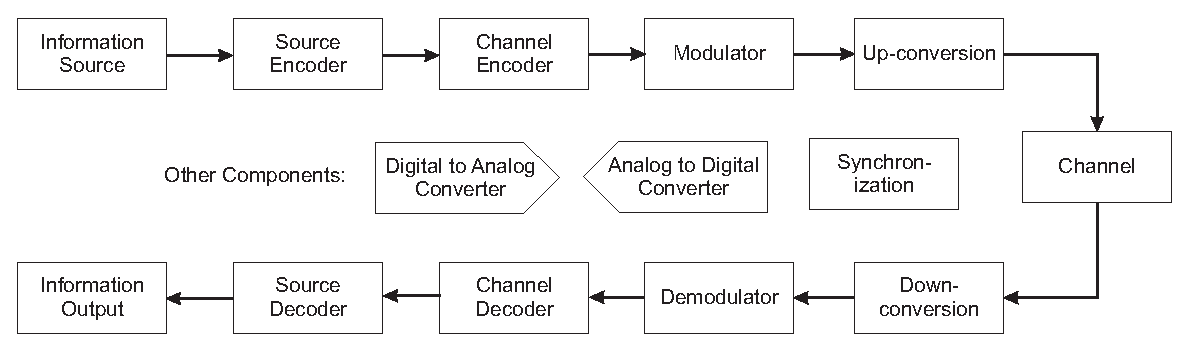
\includegraphics[width=\textwidth]{../images/Tx-Channel-Rx-Block-Diagram.eps}
  \caption{Block diagram of a single-user digital communication system, including (top) transmitter (TX), (middle) channel, and (bottom) receiver (RX).}
  \label{F:Tx-Rx-Blocks}
\end{figure}

Notes:
\begin{itemize}
  \item Information source comes from higher networking layers.  It
  may be continuous or packetized.
  %
  \item Source Encoding:  Finding a compact digital representation for
  the data source.  Includes sampling of continuous-time signals,
  and quantization of continuous-valued signals.  Also includes
  compression of those sources (lossy, or lossless).  What are some
  compression methods that you're familiar with? 
  %
  \item Channel encoding refers to redundancy added to the signal
  such that some bit errors can be later be corrected by the channel decoder.  
  %
  \item Modulation refers to the digital-to-analog conversion which
  produces a continuous-time signal that can be sent on the physical
  channel.  It is analogous to impedance matching - proper matching of a
  modulation to a channel allows optimal information transfer, like impedance
  matching ensured optimal power transfer.    Modulation and demodulation
  will be the main focus of this course.
  %
  \item Channels: See above for examples.  Typical models are
  additive noise, or linear filtering channel.
\end{itemize}

Why do we do both source encoding (which compresses the signal as
much as possible) and also channel encoding (which adds redundancy
to the signal)?  Shannon's source-channel coding
separation theorem says that (given enough time) we can do both and yet
consider them separately, without any loss.  And separation,
like layering, reduces complexity to the designer.  We will introduce source and channel encoding and decoding towards the end of this semester.  Each could be (and is) a semester course in itself.


\subsection{Channels}

A channel can often be modeled as a linear filter with the
addition of noise.  The noise comes from a variety of sources, but
predominantly:
\begin{enumerate}
  \item Thermal background noise:  Due to the physics of living
  above 0 Kelvin.  Well modeled as Gaussian, and constant across frequency.  It is
  commonly referred to as additive white Gaussian noise (AWGN).  The ``white'' color moniker comes from being constant across frequency, however, note that white, gray, and black are all colors
  that are constant across frequency.  I will typically refer to the noise as ``additive uncorrelated Gaussian'' which I feel is more precise.
  \item Interference from other transmitted signals.  These other
  transmitters whose signals we cannot completely cancel, we lump
  into the `interference' category.  These may result in non-Gaussian
  noise distribution, and  noise spectral density that varies with frequency.
\end{enumerate}
The linear filtering of the channel results from the physics and EM
of the medium.  For example, attenuation in telephone wires varies
by frequency.  Narrowband wireless channels experience fading that
varies as a function of frequency.  Wideband wireless
channels display multipath, due to multiple time-delayed
reflections, diffractions, and scattering of the signal off of the
objects in the environment.  All of these can be modeled as linear
filters.  

The filter may be constant, or time-invariant, if the medium, the TX
and RX do not move or change.  There may be slow movement of the TX or RX which causes the
channel may change slowly over time.  Even for a stationary TX
and RX, in real wireless channels, movement of cars, people, trees,
etc. in the environment may change the channel slowly over time.  For rapidly movement in a wireless channel, we will experience Doppler spreading, which is a non-linear effect, in which case our channel is neither linear nor time-invariant.

\begin{figure}[htbp]
  \centerline{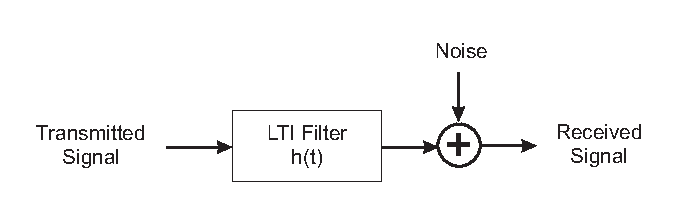
\includegraphics[width=\textwidth]{../images/Channel-Detail-Diagram.eps}}
  \caption{Linear filter and additive noise channel model.}
  \label{F:Channel-Blocks}
\end{figure}

In this course, we will focus primarily on the additive noise channel, but we
will mention what variations exist for particular channels, and how
they are addressed.

\subsection{Topic:  Random Processes}

What are things that can be considered random in a communication system?

\Solution{
Random things in a communication system:
\begin{itemize}
  \item Noise in the channel
  \item Signal (bits)
  \item Channel filtering, attenuation, and fading
  \item Device frequency, phase, and timing offsets
\end{itemize}
These random signals often pass through LTI filters, and are
sampled.  
}

We want to build the best receiver possible despite the random impediments.  Optimal
receiver design is something that we study using probability theory.

We have to tolerate errors.  Noise and attenuation of the channel
will cause bit errors to be made by the demodulator and even the
channel decoder.  This may be tolerated, or a higher layer
networking protocol (\eg, TCP) can determine that an error
occurred and then re-request the data.

\subsection{Topic:  Frequency Domain Representations}

To fit as many signals as possible onto a channel, we often split
the signals by frequency.  The concept of sharing a channel is
called \emph{multiple access} (MA).  Separating signals by frequency
band is called frequency-division multiplexing (FDM) or frequency domain multiple access (FDMA).  For the
wireless channel, this is controlled by the FCC (in the US) and
called spectrum allocation. There is a tradeoff between frequency
requirements and time requirements, which will be a major part of
this course.  The Fourier transform of our modulated, transmitted
signal is used to show that it meets the spectrum allocation limits
of the FCC.

\subsection{Topic:  Orthogonality and Signal Space}

To show that signals sharing the same channel don't interfere with
each other, we need to show that they are \emph{orthogonal}.  This
means, in short, that a receiver can uniquely separate them. Signals
in different frequency bands are orthogonal.

We can also employ multiple orthogonal signals in a single
transmitter and receiver, in order to provide multiple independent
means (dimensions) on which to modulate information.  We'll send signals that are orthogonal to the signals we send at a later time, so that we can convey different information over time and not have our own information signal interfere with itself.

We'll use signal spaces to show graphically the
results, as the example in Figure \ref{F:MPSK-signalSpaceDiagram}.  In general, we will evaluate the performance of systems which \emph{send and receive linear combinations of orthogonal signals} in order to convey digital information.

\begin{figure}[htbp]
  \centerline{
  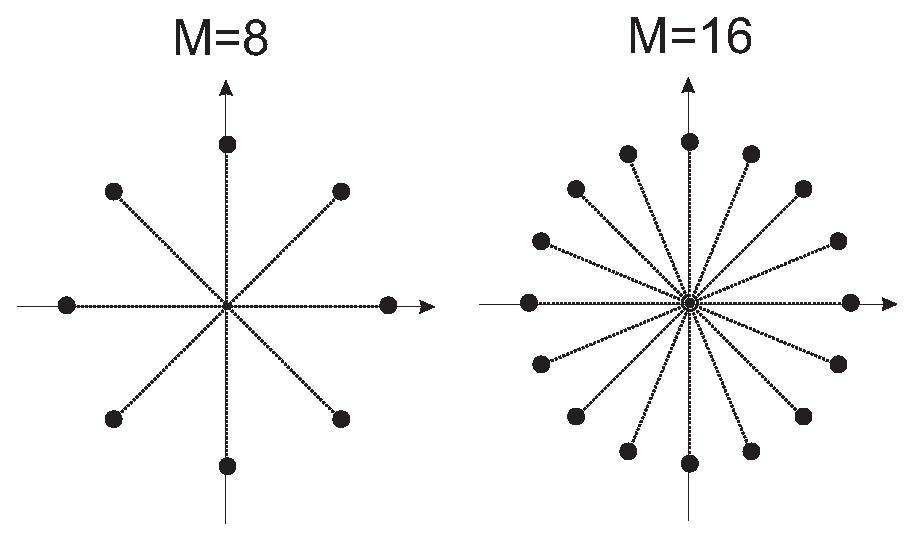
\includegraphics[width=0.8\textwidth]
  {../images/MPSK-signalSpaceDiagram.eps}
  }
  \caption{Example signal space diagram for $M$-ary Phase Shift Keying, for (a) $M=8$ and (b) $M=16$.
           Each point is a vector which can be used to send a 3 or 4 bit sequence.}
  \label{F:MPSK-signalSpaceDiagram}
\end{figure}

\subsection{Is there a need for Communications Engineers?}

Cisco's forecast (VNI Complete Forecast Highlights, \url{https://www.cisco.com/c/m/en_us/solutions/service-provider/vni-forecast-highlights.html}) says that we'll be sending 400 GB of data per capita in the US by next year, and IP traffic will triple every 5 years.  Mobile (wireless) traffic will increase twice as fast as wired.  We will not achieve these data rates using the same protocols that we have today.  Further the spectrum is well utilized; there is little additional bandwidth available to handle this rate of increase, so engineers will have to make communication systems more spectrum efficient, or make use of spectrum that is currently available at higher frequencies (20 GHz and above) where there is more spectrum available.  

Further the number of wireless devices we use are increasing rapidly.  These devices may have lower data rates (e.g., wireless thermostats) and should be able to operate with low energy consumption.  However today's  standard protocols (e.g., WiFi) do not allow them to operate in an energy efficient manner, and the protocols themselves operate inefficiently when serving large numbers of devices.  There will be multiple new generations of wireless protocols to handle our Internet-of-Things devices and allow them to be as efficient as they need to be.

Finally, the main objective of digital communications is to build systems in which we can reliably \emph{classify} information at a receiver.  A receiver must take in high-dimensional noisy measurements and make a decision about what is true about the information that was encoded.  Thus I argue that ESE 471 is the original course in ``big data''.  Information theory is still a fundamental tool in statistical machine learning, and digital communications is the background material for information theory.

%\subsection{Related classes}
%
%\begin{enumerate}
%\item Pre-requisites: Random Processes; Signals and Systems.
%\item Signal Processing:  Digital Signal Processing
%\item Electromagnetics:  EM Waves, Microwave Engineering, Antenna Theory, 
%\item Breadth: Wireless Communications Systems
%\item Devices and Circuits:  Fundamentals of Digital System Design, Analog IC Design \item Networking:  Embedded System Design,  Computer Networks
%\item Advanced Classes:  Software Radio, Information Theory,  Error Control Coding, Estimation Theory
%\end{enumerate}




\StartOf{Lecture 2}

\Today{ (1) Power, Energy, dB, (2) Orthogonality, (3) Periodicity and Impulse Functions}

%\announcements{}

\section{Power and Energy}


Two of the biggest limitations in communications systems are (1) \textit{energy} / \textit{power}; and (2) \textit{bandwidth}.  This section provides some tools to deal with power and energy.


Recall that energy is power times time.  \textbf{Use the units}:  energy is measured in Joules (J); power is measured in Watts (W) which is the same as Joules/second (J/sec).  Also, recall that our standard in signals and systems is define our signals, such as $x(t)$, as voltage signals (V).  When we want to know the power of a signal we assume it is being dissipated in a 1 Ohm resistor, so $|x(t)|^2$ is the power dissipated at time $t$ (since power is equal to the voltage squared divided by the resistance).  The actual received power a

A signal $x(t)$ has energy defined as
\[
E = \int_{-\infty}^\infty |x(t)|^2 dt
\]
A signal with finite energy is called a \emph{waveform} or \emph{energy signal}.  
For some signals, $E$ will be infinite because the signal is
non-zero for an infinite duration of time (it is always on).  These
signals we call {\it power signals} and we compute their power as
\[
  P = \limin{T} \frac{1}{2T} \int_{-T}^T |x(t)|^2 dt
\]



\subsection{Discrete-Time Signals}

In the Rice book, we refer to discrete samples of the sampled signal $x$
as $x(n)$.  You may be more familiar with the $x[n]$ notation.  But,
Matlab uses parentheses also; so we'll follow the Rice text
notation.  Essentially, whenever you see a function of $n$ (or $k$, $l$, $m$), it is a discrete-time function; whenever you see a function of $t$ (or perhaps $\tau$) it is a continuous-time function.  I'm sorry this is not more obvious in the notation.

For discrete-time signals, energy and power are defined as:
\begin{eqnarray}
  E &=& \sum_{n=-\infty}^\infty |x(n)|^2 \\
  P &=& \limin{N} \frac{1}{2N+1} \sum_{n=-N}^N |x(n)|^2
\end{eqnarray}


\subsection{Decibel Notation}

We often use a decibel (dB) scale for power.  If $P_{lin}$ is the
power in Watts, then the power in dBW is
\[
  \dBW{P} = 10 \log_{10} \frac{P_{lin}}{1 \mbox{ W}}.
\]
We convert from dB to linear by inverting the above formula,
\[
  P_{lin} = (1 \mbox{ W}) 10^{\dBW{P}/10} .
\]

Decibels are more general - they can apply to other unitless
quantities as well, such as a gain (loss) $L(f)$ through a filter
$H(f)$,
\begin{equation} \label{E:filterGaindB}
  \dB{L(f)} = 10 \log_{10} |H(f)|^2
\end{equation}

Note: Why is the capital B used?  The `Bel' refers to a Alexander Graham
`Bell' so it is capitalized.  The Bel is defined as the $\log_{10}$ of the ratio, so following the SI convention, the decibel is ten times that. The standard is to use the
decibel $10 \log_{10} (\cdot)$ which is then abbreviated as dB, just like milliwatt is abbreviated mW in the SI system.

Note that (\ref{E:filterGaindB}) could also be written as:
\begin{equation} \label{E:filterGaindB2}
  \dB{L(f)} = 20 \log_{10} |H(f)|
\end{equation}
Be careful with your use of 10 vs.~20 in the dB formula.  
\begin{itemize}
 \item Only use 20 as the multiplier if you are converting from voltage to power; \ie, taking the $\log_{10}$ of a voltage and expecting the result to be a dB power value.
\end{itemize}

Our standard is to consider power gains and losses, not voltage gains and losses.  So if we say, for example, the channel has a loss of 20 dB, this refers to a loss in power.  In particular, the output of the channel has 100 times less power than the input to the channel.

Remember these two dB numbers:
\begin{itemize}
  \item 3 dB:  This means the number is double in linear terms.
  \item 10 dB:  This means the number is ten times in linear terms.
\end{itemize}
And maybe this one:
\begin{itemize}
  \item 1 dB:  This means the number is a little over 25\% more (multiply by 5/4) in linear terms.
\end{itemize}
With these three numbers, you can quickly convert losses or gains between
linear and dB units without a calculator.  Just convert any dB number into a sum of multiples of 10, 3, and 1.

\Example{Convert dB to linear values:}
\begin{enumerate}
 \item 30 dBW
 \item 33 dBm
 \item -20 dB
 \item 4 dB
\end{enumerate}
\Solution{
\begin{enumerate}
 \item $(1 \mbox{ W}) 10^{\dBW{30}/10} = 10^3 \mbox{W} = 1000$ W.
 \item 33 dBm = 30 dBm + 3 dB = 1000 mW $\times 2$ = 2 W.
 \item -20 dB = $10^{\dBW{-20}/10} = 10^{-2} = 0.01$.
 \item 4 dB = 3 dB + 1 dB $\approx 2(1.25) =2.5$.
\end{enumerate}
}

\Example{Convert linear values to dB:}
\begin{enumerate}
 \item 0.2 W
 \item 40 mW
\end{enumerate}
\Solution{
\begin{enumerate}
 \item 0.2 W $= (0.1 \mbox{W})(2) = \dBW(-10) + \dB{3} = -7$ dBW
 \item 40 mW $= (10 \mbox{mW})(2)(2) = \dBm{10} + \dB{3} + \dB{3} = \dBW{16}$.
\end{enumerate}
}
\Example{Convert power relationships to dB:}  Convert the expression to one which involves only dB terms.
\begin{enumerate}
 \item $P_{y,lin} = 100 P_{x,lin}$
 \item $P_{o,lin} = G_{connector,lin} L_{cable,lin}^{-d}$, where $P_{o,lin}$ is the received power in a fiber-optic link, where $d$ is the cable length (typically in units of km), $G_{connector,lin}$ is the gain in any connectors, and $L_{cable,lin}$ is a loss in a 1 km cable.
 \item $P_{r,lin} = P_{t,lin} \frac{G_{t,lin} G_{t,lin} \lambda^2}{(4\pi d)^2}$, where $\lambda$ is the wavelength (m), $d$ is the path length (m), and $G_{t,lin}$ and $G_{t,lin}$ are the linear gains in the antennas, $P_{t,lin}$ is the transmit power (W) and $P_{r,lin}$ is the received power (W).  This is the Friis free space path loss formula.
\end{enumerate}

These last two are what we will need in Section 6.4, when we discuss link budgets.  The main idea is that we have a limited amount of power which will be available at the receiver.



\section{Orthogonality}
In the introductory lecture, we described a couple reasons why orthogonal signals are used in digital communication systems.  In short, we use orthogonal signals for:
\begin{enumerate}
 \item \emph{Multiple Access}: Multiple users can access the same medium, and a receiver can separate one user's signal from the rest.
 \item \emph{Increasing Signal Dimension}: A single user can send information along multiple dimensions at the same time, which is useful for increasing the bit rate or fidelity.
\end{enumerate}

Also, I gave  my ``engineering'' definition of a set of orthogonal waveforms:  \emph{They are waveforms that can be separated at the receiver.}  Now, let's provide the mathematical definition.

\Definition{Orthogonal}{  Two real-valued waveforms $\phi_0(t)$ and $\phi_1(t)$ are
\textit{orthogonal} if
\[
  \int_{-\infty}^\infty \phi_0(t)\phi_1(t) dt = 0.
\] 
Two complex-valued waveforms $\phi_0(t)$ and $\phi_1(t)$ are orthogonal if
\[
  \int_{-\infty}^\infty \phi_0(t) \phi_1^*(t) dt = 0,
\] 
where $\phi_1^*(t)$ is the complex conjugate of $\phi_1(t)$.
}

What does this integral remind you of?

\Definition{Orthogonal Set}{$K$ waveforms $\phi_0(t), \ldots, \phi_{K-1}(t)$ are
mutually orthogonal, or form an orthogonal set, if every pair of waveforms $\phi_i(t)$, $\phi_j(t)$, for $i\neq j$, is orthogonal.}

\Example{Sine and Cosine} Let
\begin{eqnarray}
 \phi_0(t) &=& \pdfarray{\cos(2\pi t)}{0< t \le 1} \nonumber \\
 \phi_1(t) &=& \pdfarray{\sin(2\pi t)}{0< t \le 1} \nonumber
\end{eqnarray}
Are $\phi_0(t)$ and $\phi_1(t)$ orthogonal?

\Solution{
Using $\sin 2x = 2 \cos x \sin x$, 
\begin{eqnarray}
  \int_{-\infty}^\infty \phi_0(t)\phi_1(t) dt  &=& \int_0^1 \cos(2\pi t)\sin(2\pi t)dt  \nnn
   &=&\int_0^1 \frac{1}{2}\sin(4\pi t)dt \nnn
   &=& \left. \frac{-1}{8\pi}\cos(4\pi t)\right|_0^1 = \frac{-1}{8\pi}(1-1) = 0  \nn
\end{eqnarray}
So, yes, $\phi_0(t)$ and $\phi_1(t)$ are orthogonal.
}

\Example{Frequency Shift Keying}  Assume $T_s >> 1/f_c$, and show that these two are orthogonal.
\begin{eqnarray} \label{E:FSK-Symbols}
 \phi_0(t) &=& \pdfarray{\cos \left(2\pi f_c t  \right)}{0 \le t \le T_s} \nnn
 \phi_1(t) &=& \pdfarray{\cos \left( 2\pi \left[f_c + \frac{1}{T_{s}}\right] t \right)}{0 \le t \le T_s} \nn
\end{eqnarray}

\Solution{ The integral of the product of the two must be zero.  Checking, and using the identity for the product of two cosines,
\begin{eqnarray} \label{E:FSK-Symbols2}
 && \int_0^{T_s} \cos \left(2\pi f_c t  \right) \cos \left( 2\pi \left[f_c + \frac{1}{T_{s}}\right] t \right)  dt
\nnn
 &=& \frac{1}{2}\int_0^{T_s} \cos \left(2\pi t/T_s  \right) dt + \frac{1}{2} \int_0^{T_s} \cos \left( 4\pi f_c t + 2\pi t/T_{s} \right)  dt
\nnn
 &=& 0 + \frac{1}{2}\left[ \frac{1}{2 \pi (2f_c + 1/T_s)} \sin \left( 2\pi ( 2 f_c + 1/T_{s}) t \right) \right|_0^{T_s}  
\nn
\end{eqnarray}
The remaining term has a $\frac{1}{2 \pi (2f_c + 1/T_s)}$ constant out front.  Because $f_c$ is very high, this term will be very very low.  The sine term is limited to between -1 and +1 so it will not cause the second term to be large.  Thus,
\begin{eqnarray} \label{E:FSK-Symbols3}
\int_{-\infty}^\infty \phi_0(t)\phi_1(t) dt   \le  \frac{1}{ \pi (2f_c + 1/T_s)} &\approx&  0
\nn
\end{eqnarray}
Thus the two different frequency waveforms are orthogonal.
}

\subsection{Linear Combinations}

What is a linear combination of orthogonal waveforms?  Well, consider the orthogonal set $\phi_0(t), \ldots, \phi_{K-1}(t)$.  A linear combination $s_m(t)$ is
\[
 s_m(t) = a_{m,0} \phi_0(t) + a_{m,1} \phi_1(t) + \cdots + a_{m,K-1} \phi_{K-1}(t) = \sum_{m=k}^{K-1} a_{m,k} \phi_k(t)
\]
We also call the a linear combination a {\it symbol}.  We use subscript $m$ to indicate that it's not the only possible linear combination (or symbol).  In fact, we will use $M$ different symbols, so $i=0, \ldots, M-1$, and we will use $s_0(t), \ldots, s_{M-1}(t)$.

We represent the $m$th symbol (linear combination of the orthogonal waveforms), $s_m(t)$, as a vector for ease of notation:
\[
\mbs_m = [a_{m,0}, a_{m,1}, \ldots, a_{m,K-1}]^T 
\]
The superscript $T$ is for transpose -- $\mbs_m$ is a column vector.  Vectors are easy to deal with because they can be plotted in vector space, to show graphically what is going on.  We call the plot of all possible $\mbs_m$, that is, for $m=0, \ldots M-1$, the \textit{constellation diagram}.  Some examples are shown in Figure \ref{F:MPSKEg}.


\subsection{Using $M$ Different Linear Combinations}

Here is how a transmitter \emph{uses} the different linear combinations to convey digital bits to the receiver.  First, consider that there are $M$ different symbols for the TX to chose from.  Each symbol is described by a $\log_2 M$-length bit sequence.  For example, if there are $8$ possible combinations, we would label them 000, 001, 011, 010, 110, 111, 101, 100.  

The transmitter knows which $\log_2 M$-bit sequence it wants to send.  It picks the symbol that corresponds to that bit sequence, let's call it symbol $m$.  Then it sends $s_m(t)$.  

If the receiver is able to determine that symbol $m$ was sent, it will correctly receive those $\log_2 M$ bits of information.  In this example, it will receive three bits of information.


\begin{figure}[htbp]
  \centerline{(a)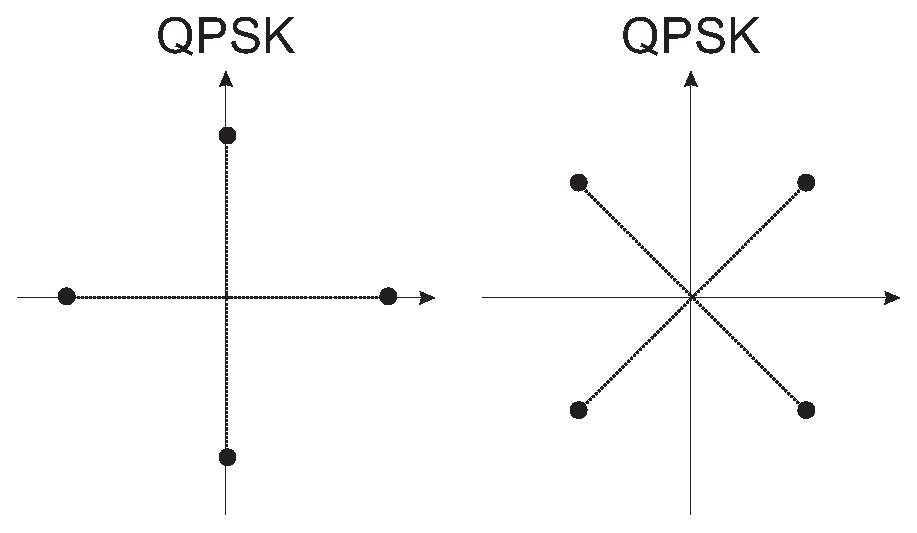
\includegraphics[width=0.6\textwidth]{../images/QPSK-signalSpaceDiagram.eps}
  }
  \centerline{(b)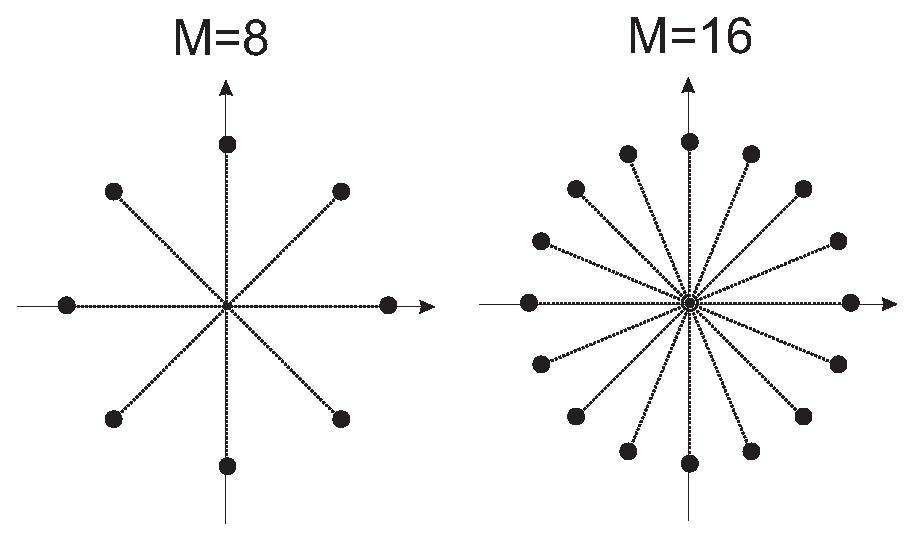
\includegraphics[width=0.6\textwidth]{../images/MPSK-signalSpaceDiagram.eps} }
  \centerline{(c)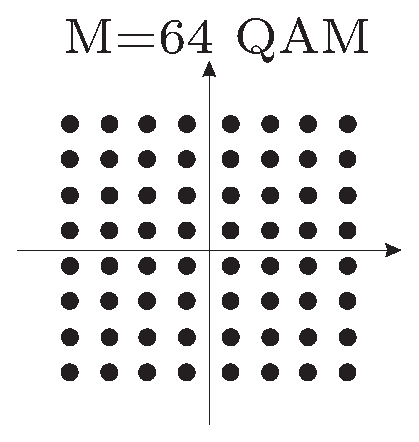
\includegraphics[width=0.3\textwidth]{../images/QAM64Eg.eps} }
  \caption{Signal constellations for (a) $M=4$ PSK (a.k.a. BPSK), (b) $M=8$ and $M=16$ PSK, and (c) 64-QAM.}
  \label{F:MPSKEg}
\end{figure}

In the next lecture we will talk about how a receiver is able to separate the received signal into components, each corresponding to one of the orthogonal waveforms $\phi_k(t)$.  From this separation, it will be able to decide which symbol was sent.


\subsection{How to Choose a Modulation}

A \textit{digital modulation} is the choice of: (1) the  linear combinations $\mbs_0, \ldots, \mbs_{M-1}$ and, (2) the orthogonal waveforms $\phi_0(t), \ldots, \phi_{K-1}(t)$.  We will choose a digital modulation as a tradeoff between the following characteristics:
\begin{enumerate}
 \item Bandwidth efficiency: How many bits per second (bps) can be sent per Hertz of signal bandwidth.  Thus the bandwidth efficiency has units of bps/Hz.
 \item Power efficiency: How much energy per bit is required at the receiver in order to achieve a desired fidelity (low bit error rate).  We typically use $S/N$ or $E_s/N_0$ or $E_b/N_0$ as our figure of merit.  This will be a major topic of the 2nd part of this course.
 \item Cost of implementation:  Things like symbol and carrier synchronization, and linear transmitters, require additional device cost, which might be unacceptable in a particular system.
\end{enumerate}




\section{Time-Domain Concept Review}

\subsection{Periodicity}

\Definition{Periodic (continuous-time)}{A signal $x(t)$ is periodic if $x(t) =
x(t+T_0)$ for some constant $T_0 \neq 0$ for all $t\in \mR$. The
smallest such constant $T_0>0$ is the \emph{period}.}

If a signal is not periodic it is {\it aperiodic}.

Periodic signals have Fourier series representations, as defined in Rice Ch.~2.


\Definition{Periodic (discrete-time)}{A DT signal $x(n)$ is periodic if $x(n) = x(n+N_0)$ for some integer
$N_0\neq 0$, for all integers $n$.  The smallest positive integer 
$N_0$ is the period.}


\subsection{Impulse Functions}

\Definition{Impulse Function}{The (Dirac) impulse function
$\delta(t)$ is the function which makes
\begin{equation} \label{E:impulseFunctionDefn}
  \int_{-\infty}^\infty x(t)\delta(t) dt = x(0)
\end{equation}
 true for any function $x(t)$ which is continuous at $t=0$.}

We are defining a function by its most important property, the
`sifting property'.  Is the following definition more
familiar?
\[
  \delta(t) = \lim_{T\rightarrow 0} \pdfarray{1/(2T)}{-T \le t \le T}
\]
You can visualize $\delta(t)$ here as an infinitely high,
infinitesimally wide pulse at the origin, with area one.  This is
why it `pulls out' the value of $x(t)$ in the integral in
(\ref{E:impulseFunctionDefn}).

Other properties of the impulse function:
\begin{itemize}
  \item Time scaling,
  \item Symmetry,
  \item Sifting at arbitrary time $t_0$,
\end{itemize}

The continuous-time unit step function is
\[
 u(t) = \pdfarray{1}{t\ge 0}
\]


\Example{Sifting Property} What is $\int_{-\infty}^\infty \frac{\sin
(\pi t)}{\pi t} \delta(1-t) dt$?

\Solution{The integral pulls out the value of the fraction when the argument of the $\delta $ function is zero, in this case, when $t=1$.  Thus plug in $t=1$ into $\frac{\sin
(\pi t)}{\pi t}$ and get $\frac{\sin
(\pi)}{\pi} = 0/\pi = 0$.}

The discrete-time impulse function (also called the Kronecker delta
or $\delta_K$) is defined as:
\[
 \delta(n) = \pdfarray{1}{n=0}
\]
(There is no need to get complicated with the math; this is well
defined.)  Also,
\[
 u(n) = \pdfarray{1}{n\ge 0}
\]





 
 


\StartOf{Lecture 3}

\Today{Orthogonal Signal Representations: (1) Span, (2) Synthesis, (3) Analysis}

\announcements{
\begin{itemize}
  \item For today:  Rice 5.1; For Mon: Rice 2.5-2.7 and Rice 6.2.1.
  \item HW 1 due a week from today at 11:59pm
  \item Office hours Friday 2:30-3:45pm; please email or use the discussion board for HW questions next week.
  \item I'm out of the country for a conference Mon-Thu next week. Dr.\ Alemayehu Solomon Abrar will be doing a lecture on Mon Jan 27.  There will be no class on Wed Jan 29.
\end{itemize}
}

\section{Orthonormal Signal Representations}

%Last time we defined the term ``orthogonal'' for a pair or set of functions.  I mentioned that a transmitter has a list of possible symbols to send (linear combinations of these waveforms); and that a receiver can estimate the particular amount of each waveform that was sent.  Today we are going to present \emph{how} the transmitter and receiver do both of these things.

We've been talking about orthogonal waveforms. A shorthand notation: the integral of the product of two functions is also called the inner product, and sometimes the notation is used, where $f(t)$ and $g(t)$ are two waveforms:
\[
 \langle f(t), g(t) \rangle = \intinfty{t}{f(t) g(t)}
\]

Recall the definition of an orthonormal basis as given in the previous lecture.

\Definition{Orthonormal}{A set of functions $\phi_0(t), \ldots, \phi_{K-1}(t)$ are \emph{orthonormal} (also referred to as an \emph{orthonormal basis}) if they are mutually orthogonal and each has unit energy, \ie, $\intinfty{t}{ |\phi_k(t)|^2} = 1$ for $k=0,1$.}

Sometimes an orthonormal basis is also called an orthonormal set. There is no difference between the two terms.  The word ``basis'' is nice because it implies you can build something out of the set -- and in fact, you can build a variety of signals by taking some linear combination of the functions in the orthonormal basis.  

For shorthand, we use a set name to describe the orthonormal basis.  The Rice book uses $\mathcal{B}$:
\[
 \mathcal{B} = \{ \phi_0(t), \phi_1(t), \ldots, \phi_{K-1}(t) \}
\]

Each function in $\mathcal{B}$ is called a basis function. You can
think of $\mathcal{B}$ as an unambiguous and useful language.  

What are some common orthonormal bases?
\begin{itemize}
 \item Nyquist sampling: sinc functions centered at sampling times.
 \item Fourier series: complex sinusoids at different frequencies
 \item Sine and cosine at the same frequency
 \item Wavelets
\end{itemize}
And, we will come up with others.  Each one has a limitation -- only a certain set of signals can be exactly represented as a linear combination of its waveforms.  Essentially, we must limit the set of possible signals to a set.  That is, some subset of all possible signals.


\subsection{Span of an Orthonormal Basis}

\Definition{Span}{The span of the set $\mathcal{B}$ is the set of
all functions which are linear combinations of the functions in
$\mathcal{B}$.  The span is referred to as $\Span{B}$ and is
\[
 \Span{B} = \left\{ \sum_{k=0}^{K-1} a_k \phi_k(t)  \mbox{ such that } a_0, \ldots,
 a_{K-1} \in \mathbb{R} \right\}
\]
Another way to define this set is to say that a function $f(t)\in \Span{B}$ if and only if there exists $a_0, \ldots, a_{K-1} \in \mathbb{R}$ such that 
 \[
  f(t) = \sum_{k=0}^{K-1} a_k \phi_k(t)
 \]
}

Recall that we said in Lecture 2 that our modulation scheme is a set of $M$ different linear combinations of $\phi_0(t)$ through $\phi_{K-1}(t)$.  In particular, our transmitter will select symbols of the form
\[
 s_m(t) = a_{m,0} \phi_0(t) + a_{m,1} \phi_1(t) + \cdots + a_{m,K-1} \phi_{K-1}(t) 
\]
for $m=0$ to $M-1$.  Clearly, all symbols $s_m(t) \in \Span{B}$.  We call the set of the $M$ possible symbols $\mathcal{S}$.  That is,
\[
 \mathcal{S} = \{ s_0(t), \ldots, s_{M-1}(t)\}.
\]
Since every element of $ \mathcal{S} \in \Span{B}$, it is clear that $ \mathcal{S} \subset \Span{B}$.


\subsection{Synthesis}

Consider that you have a symbol waveform you want to send, $s_m(t)$, and that you know that it is in the span of your basis $\mathbf{B}$.  Then it can be represented
as a linear combination of the basis functions,
\[
  s_m(t) = \sum_{k=0}^{K-1} a_{m,k} \phi_k(t)
\]
Further, we can calculate the particular constants $a_{m,k}$ using the inner product:
\[
  a_{m,k} = \langle s_m(t), \phi_k(t) \rangle
\]
The \emph{projection} of the $m$th symbol $s_m(t)$ onto basis function $k$ is
defined as $a_{m,k} \phi_k(t) = \langle s_m(t), \phi_k(t) \rangle
\phi_k(t)$. Then the signal is equal to the sum of its projections
onto the basis functions.

\textbf{Why is this?}

\Solution{ Since $s_m(t) \in \Span{B}$, we know there are some
constants $\{a_{m,k}\}_k^{K-1}$ such that
\[
   s_m(t) =  \sum_{k=0}^{K-1} a_{m,k} \phi_k(t)
\]
Taking the inner product of both sides with $\phi_j(t)$,
\begin{eqnarray}
  \langle s_m(t), \phi_j(t) \rangle &=&
     \left\langle \sum_{k=0}^{K-1} a_{m,k} \phi_k(t), \phi_j(t) \right\rangle \nnn
  \langle s_m(t), \phi_j(t) \rangle &=&
     \sum_{k=0}^{K-1} a_{m,k} \langle \phi_k(t), \phi_j(t) \rangle \nnn
  \langle s_m(t), \phi_j(t) \rangle &=&  a_{m,j} \nn
\end{eqnarray}
}

So, now we can now represent a signal by a vector,
\[
  \mbs_i = [ a_{i,0}, a_{i,1}, \ldots, a_{i,K-1}]^T
\]
This and the basis functions \textbf{completely represent each
signal}. Plotting $\{\mbs_i\}_i$ in an $K$ dimensional grid is
termed a \emph{constellation diagram}.  Generally, this space that
we're plotting in is called \emph{signal space}.

We can also synthesize any of our $M$ signals in the signal set by
adding the proper linear combination of the $K$ orthonormal waveforms.  By choosing
one of the $M$ signals, we convey information, specifically, $\log_2
M$ bits of information.  


\begin{figure}[htbp]
  \centerline{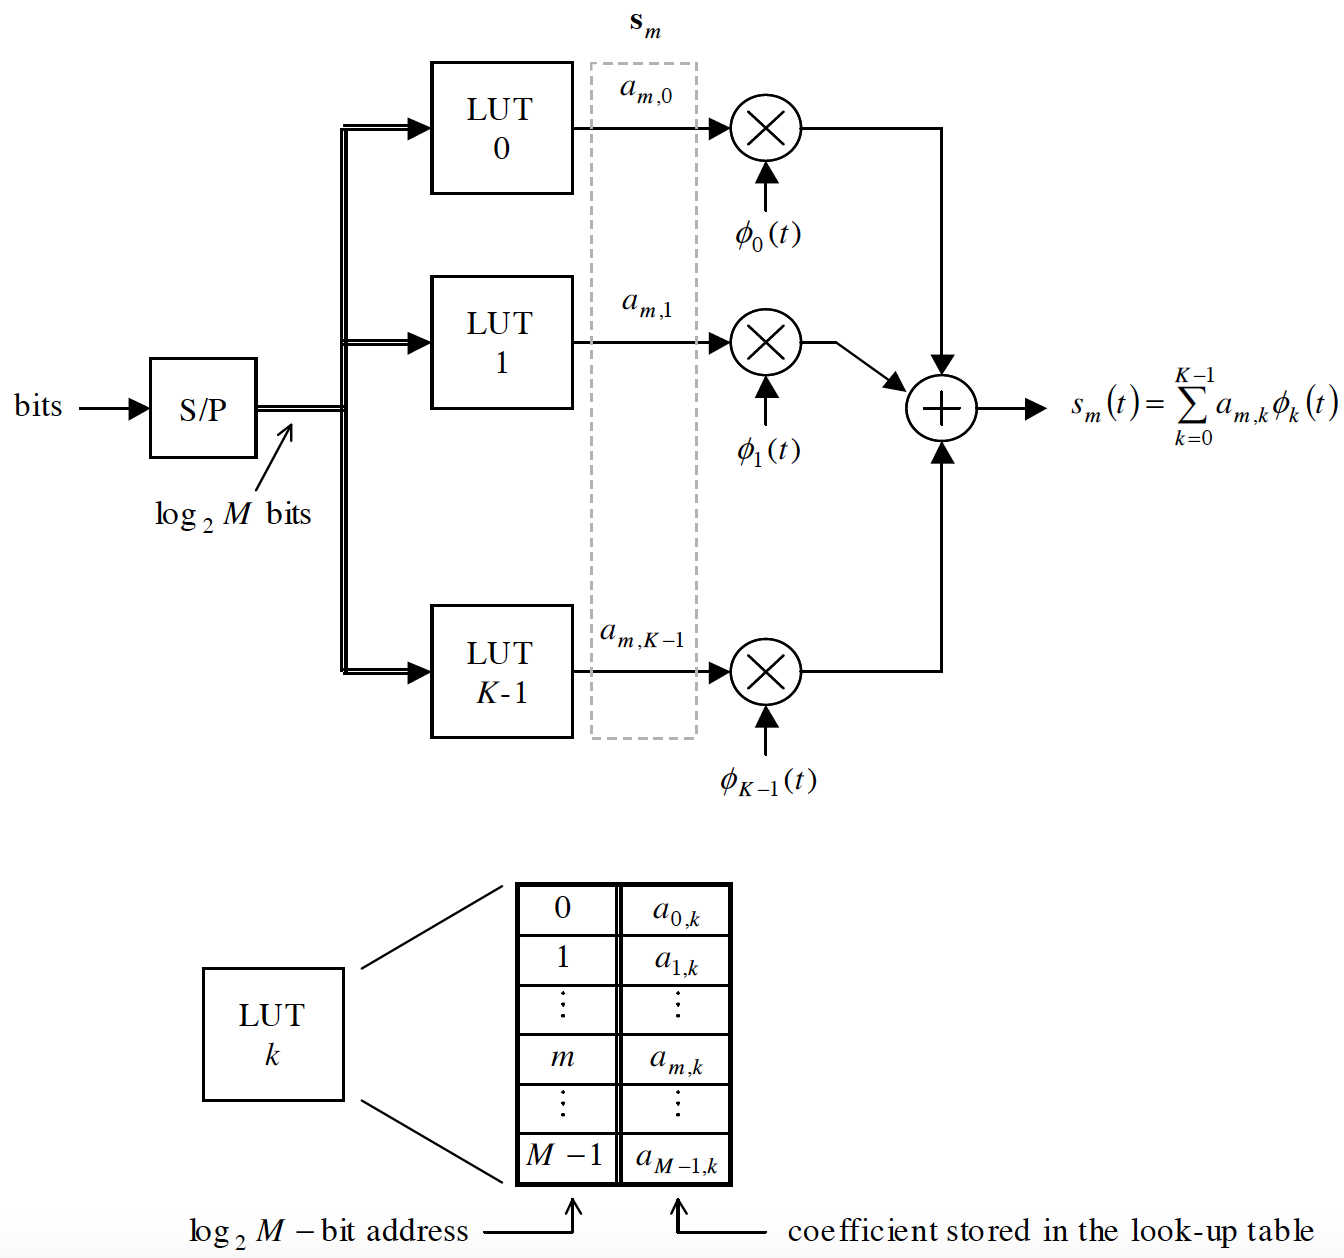
\includegraphics[width=0.8\textwidth]{RiceFigure5-5.png}
  }
  \caption{Rice book Figure 5.5: Block diagram of a modulator for M-ary linear modulation based on the synthesis
equation.}
  \label{F:SynthesisEquationFig}
\end{figure}

See Figure \ref{F:SynthesisEquationFig}, from Rice Chapter 5, which shows a block diagram of how a transmitter would synthesize one of the $M$ signals to send, based on an input bitstream.


\Example{Position-shifted pulses} Plot the signal space diagram for
the signals,
\begin{eqnarray}
  s_0(t) &=& u(t) - u(t-1) \nonumber \\
  s_1(t) &=& u(t-1) - u(t-2) \nonumber \\
  s_2(t) &=& u(t) - u(t-2) \nonumber
\end{eqnarray}
given the orthonormal basis,
\begin{eqnarray}
  \phi_0(t) &=& u(t) - u(t-1) \nonumber \\
  \phi_1(t) &=& u(t-1) - u(t-2) \nonumber
\end{eqnarray}
What are the signal space vectors, $\mbs_0$, $\mbs_1$, and $\mbs_2$?

\Solution{They are $\mbs_0 = [1, 0]^T$, $\mbs_1 = [0, 1]^T$, and
$\mbs_2 = [1, 1]^T$. They are plotted in the signal space diagram in
Figure \ref{F:SampleSpacePosition}.

\begin{figure}[htbp]
  \centerline{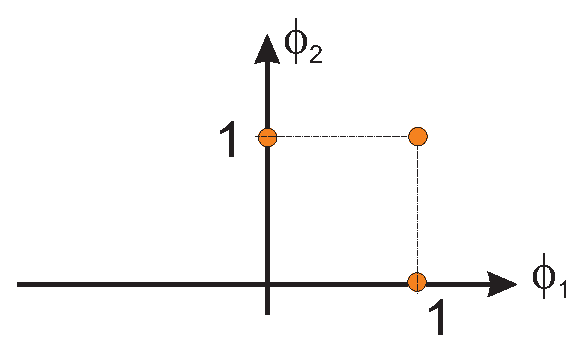
\includegraphics[width=0.4\textwidth]{../images/SignalSpaceExample1.eps}}
  \caption{Signal space diagram for position-shifted signals example.}
  \label{F:SampleSpacePosition}
\end{figure}
}

Energy:
\begin{itemize}
  \item Energy can be calculated in signal space as
    \[
      \mbox{Energy}\{s_m(t)\} = \int_{-\infty}^{\infty}  s_i^2(t) dt = \sum_{k=0}^{K-1}  a_{m,k}^2
    \]
    Proof?
  \item We will find out later that it is the distances between
    the points in signal space which determine the bit error rate
    performance of the receiver.
    \[
      d_{i,j} = \| \mbs_i - \mbs_j \| = \sqrt{\sum_{k=0}^{K-1} (a_{i,k} - a_{j,k})^2 }
    \]
    for $i,j$ in $\{0, \ldots, M-1\}$.  The norm $\| \cdot \|$ given above is the Euclidean norm.
  \item Although different orthonormal bases can be used (one can represent the same symbols with a different orthonormal basis and different symbol vectors), the energy and
    distance between points will not change.
\end{itemize}

\Example{Amplitude-shifted signals} Now consider
\begin{eqnarray}
  s_0(t) &=& 1.5[u(t) - u(t-1)] \nonumber \\
  s_1(t) &=& 0.5[u(t) - u(t-1)] \nonumber \\
  s_2(t) &=& -0.5[u(t) - u(t-1)] \nonumber \\
  s_3(t) &=& -1.5[u(t) - u(t-1)] \nonumber
\end{eqnarray}
and the orthonormal basis,
\begin{eqnarray}
  \phi_1(t) &=& u(t) - u(t-1) \nonumber
\end{eqnarray}
What are the signal space vectors for the signals $\{s_m(t)\}$? What
are their energies?


\Solution{  $\mbs_0 = [1.5]$, $\mbs_1 = [0.5]$, $\mbs_2 = [-0.5]$,
$\mbs_3 = [-1.5]$.  See Figure \ref{F:SampleSpaceAmplitude2}.

\begin{figure}[htbp]
  \centerline{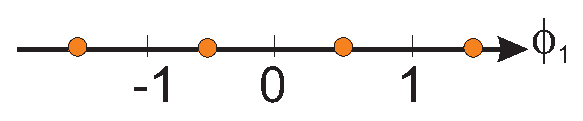
\includegraphics[width=0.4\textwidth]{../images/SignalSpaceExample2.eps}}
  \caption{Signal space diagram for amplitude-shifted signals example.}
  \label{F:SampleSpaceAmplitude2}
\end{figure}

Energies are just the squared magnitude of the vector: 2.25, 0.25,
0.25, and 2.25, respectively. }


\subsection{Analysis}

At a receiver, our job will be to analyze the received signal (a function) and to decide which of the $M$ possible signals was sent. This is the task of \emph{analysis}.  It turns out that an orthonormal bases makes our analysis very straightforward and elegant.

We won't receive exactly what we sent - there will be additional
functions added to the signal function we sent.
\begin{itemize}
  \item Thermal noise
  \item Interference from other users
  \item Self-interference (leftovers from what our transmitter recently sent)
\end{itemize}
We might say that if we send signal $m$, \ie, $s_m(t)$ from our signal set, then we would
receive
\[
  r(t) = s_m(t) + w(t)
\]
where the $w(t)$ is the sum of all of the additive signals that we
did not intend to receive.  But  $w(t)$ would generally not be totally  in the span of our basis $\mathcal{B}$, so $r(t)$ would not be in $\Span{B}$ either.  


\subsubsection{Symbol Closest to Received Signal}

One main question we ask at the receiver is, what is the symbol $s_m(t)$ that is closest to the received signal?  The term ``closest'' here is somewhat qualitative until we define it.  Without proof (in this lecture) we are going to use squared error to measure ``closeness'':
\begin{equation}
 \mathcal{E}_m = \int_{-\infty}^\infty |r(t) - s_m(t)|^2 dt
\end{equation}
That is, for any given $m$, we would integrate across time the squared difference between $r(t)$ and $s_m(t)$.  Our decision will be the $m$ that has minimum $\mathcal{E}_m$:
\begin{equation}
 \hat{m} = \arg \min_{m \in \{0 \ldots M-1\}}  
     \left\{ 
         \int_{-\infty}^\infty |r(t) - s_m(t)|^2 dt
     \right\}
\end{equation}
The term $\hat{s}(t)$ is the result, the receiver's guess of the transmitted symbol.  Because $s_m(t) \in \mathcal{S}$, we know that $s_m(t) = \sum_{k=0}^{K-1} a_{m,k} \phi_{m,k}$.  So,
\begin{eqnarray}
\hat{m} &=& \arg \min_{m \in \{0 \ldots M-1\}} 
     \left\{ 
         \intinfty{t}{ r^2(t)} \right. \nnn
  &&     - 2 \sum_{k=0}^{K-1} a_{m,k} \intinfty{t}{ r(t)\phi_k(t)}  \nnn
  && \left.
         + \sum_{k=0}^{K-1} \sum_{k'=0}^{K-1} a_{m,k} a_{m,k'} \intinfty{t}{ \phi_k(t)\phi_{k'}(t)} 
     \right\}.
\end{eqnarray}
Although there are a lot of terms, this begins to simplify.  The first term is not a function of $m$.  The integral in the second term is the inner product $\langle r(t),\phi_k(t)\rangle$.  Let's call this $x_k$.  The integral in the third term is one when $k=k'$ and zero otherwise, so we can just consider the terms when $k=k'$,
\begin{equation}
 \arg \min_{m \in \{0 \ldots M-1\}} 
     \left\{ - 2 \sum_{k=0}^{K-1} a_{m,k} x_k + \sum_{k=0}^{K-1} a^2_{m,k}
     \right\}.
\end{equation}
We can make this easier for us by including a constant $\sum_{k=0}^{K-1} x^2_k$. Since this constant is not a function of $m$, it doesn't affect the arg min.
\begin{eqnarray}
 &=& \arg \min_{m \in \{0 \ldots M-1\}} 
     \left\{ \sum_{k=0}^{K-1} \left( x^2_k - 2  a_{m,k} x_k + a^2_{m,k} \right)
     \right\}. \nnn
 &=&  \arg \min_{m \in \{0 \ldots M-1\}} 
     \left\{ \sum_{k=0}^{K-1} \left( x_k -  a_{m,k}\right)^2
     \right\}. \nnn
\end{eqnarray}
To find the $m$ that makes this the smallest, then, we should calculate the $x_k$ values by finding the inner product between the received signal and $\phi_k(t)$, and forming the vector
\[
 \mbx = [ x_0, x_1, \ldots, x_{K-1}]^T
\]
Keep a list of the symbol vectors $\mbs_m$ for each $m$.  The final expression above translates to 
\begin{equation}
\hat{m} = \arg \min_{m} \| \mbx - \mbs_m \|^2
\end{equation}
where $\| \cdot \|^2$ is the squared norm of a vector.  Thus, just find the squared Euclidean distance between each $\mbs_m$ and $\mbx$.  This lowest-squared distance vector corresponds to the $m$ that is closest to the received signal.

Note that $\mbx$, that is, the inner products 
\[
 x_k = \intinfty{t}{ r(t)\phi_k(t)}
\]
are all that matters in the decision about which symbol was sent.  



\subsubsection{Best Approximation for Received Signal in the Basis}

What is the best approximation to $r(t)$ in the
signal space?  Specifically, what is $\hat{r}(t) \in \Span{B}$ such
that the energy of the difference between $\hat{r}(t)$ and $r(t)$ is
minimized, \ie,
\begin{equation} \label{E:ProjectionError}
  \arg \min_{\hat{r}(t) \in \Span{B}} \int_{-\infty}^\infty | \hat{r}(t) - r(t) |^2 dt
\end{equation}

\Solution{ Since $\hat{r}(t) \in \Span{B}$, it can be represented as
a vector in signal space,
\[
  \mbx = [x_0, x_1, \ldots, x_{K-1} ]^T.
\]
and the synthesis equation is
\[
  \hat{r}(t) = \sum_{k=0}^{K-1} x_k \phi_k(t)
\]
If you plug in the above expression for $\hat{r}(t)$ into
(\ref{E:ProjectionError}), and then find the minimum with respect to
each $x_k$, you'd see that the minimum error is at
\[
x_k = \int_{-\infty}^\infty r(t) \phi_k(t) dt
\]
that is, $x_k = \langle r(t), \phi_k(t) \rangle$, for $k=0, \ldots,
K-1$. }

\Example{ Analysis using a Walsh-Hadamard 2 Basis}  See Figure
\ref{F:SignalSpaceAnalysisExample}.   Let $s_0(t) = \phi_0(t)$ and 
$s_1(t) = \phi_1(t)$. What is $\hat{r}(t)$?

\begin{figure}[htbp]
  \centerline{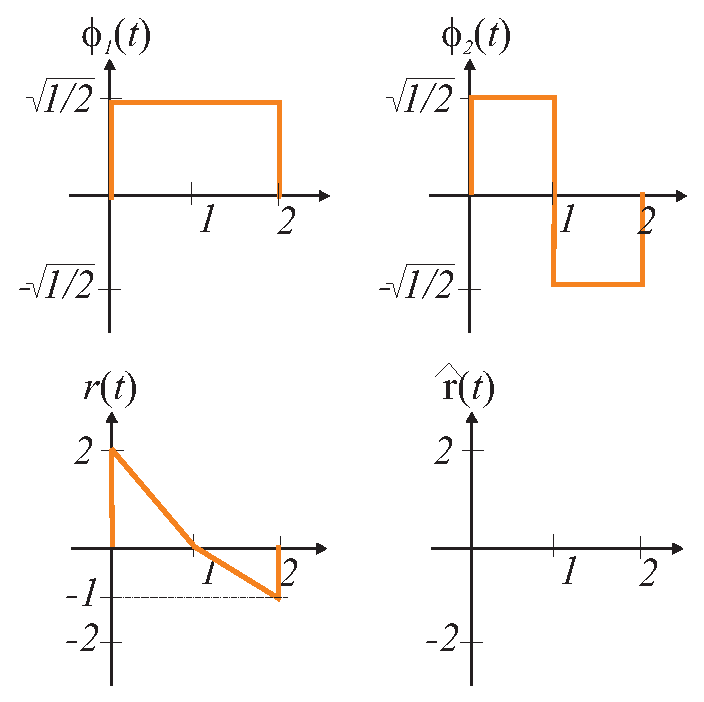
\includegraphics[width=0.6\textwidth]{../images/SigSpace-Analysis-EgProblem.eps}}
  \caption{Signal and basis functions for Analysis example.}
  \label{F:SignalSpaceAnalysisExample}
\end{figure}

\Solution{
\[
 \hat{r}(t) = \pdfarrays{1}{0 \le t < 1}{-1/2}{1 \le t < 2}
\]
}
%\section{Gram-Schmidt Algorithm}
%
%How do you come up with orthonormal bases?  This section presents
%the Gram-Schmidt algorithm.  This material is heavy in calculations,
%easy to make mistakes, and as such not required material for this
%course. But, you should know what it does so that you can use the
%equivalent Matlab script to generate an orthonormal basis.
%
%\begin{figure}[h]
%  \centerline{\psfig{figure=FourPulses-Problem-7-6.eps,width=3in}}
%  \caption{Four signals used to send 2 bits of information.}
%  \label{F:Sampling-FreqDomain}
%\end{figure}
%
%\Example{Taken from Proakis \& Salehi} Consider a transmitter which
%sends one the following transmitted waveforms in order to convey
%data. We might use $s_1(t)$ to transmit a `01', $s_2(t)$ to transmit
%a `10', $s_3(t)$ to transmit a `11', and $s_4(t)$ to transmit a
%`00'.
%\begin{enumerate}
% \item What is an orthonormal basis for these four signals?
%\end{enumerate}
%
%Solution:  Use Gram-Schmidt algorithm.
%
%Round 1:  Select signal $s_1(t)$ and normalize it to find the first
%basis function,
%\[
%  \phi_1(t) = \frac{s_1(t)}{\|s_1(t)\|}
%\]
%Then, start round $k=2$ and repeat the following steps:
%\begin{enumerate}
%  \item \emph{Compute Projections}:  Calculate the inner product of $s_{k}(t)$
%    with the basis functions so far,
%    \begin{eqnarray}
%      c_{k,1} &=& \langle s_{k}(t), \phi_1(t) \rangle \nonumber \\
%        \vdots && \vdots \nonumber \\
%      c_{k,k-1} &=& \langle s_{k}(t), \phi_{k-1}(t) \rangle \nonumber
%    \end{eqnarray}
%  \item \emph{Subtract Projections}: Calculate an
%    orthogonal function $d_k(t)$ as,
%    \begin{equation}
%      d_k(t) = s_k(t) - \sum_{i=1}^{k-1} c_{k,i} \phi_i(t)
%    \end{equation}
%  \item \emph{Check for Stopping Condition}:  If $d_k(t) = 0$ for all $t$,
%    then no new basis function is created.  If $d_k(t) \neq 0$ then
%    do the next step.
%  \item \emph{Normalize}:  Create a new basis function,
%    \[
%      \phi_k(t) = \frac{d_k(t)}{\|d_k(t)\|}
%    \]
%    Repeat 1-4 until $k=M$.
%\end{enumerate}
%The value $N$ is the number of new basis functions created.  This is
%the minimum $N$ functions which can form an orthogonal basis for
%$\{s_m(t)\}$.
%
%\Note{You can order the signals $s_m(t)$ in any order.  You may get
%different bases, but $N$ will be the same.}
%
%
%\Example{Example from Proakis \& Salehi} Starting with $s_1(t)$,
%first calculate $\phi_1(t)$:
%\[
%  \phi_1(t) = \frac{2[u(t) - u(t-3)]}{\sqrt{4\cdot 3}}
%            = \frac{u(t) - u(t-3)}{\sqrt{3}}
%\]
%Start the 4-step process.  For $k=2$,
%\begin{enumerate}
%  \item \emph{Compute Projections}:
%    \begin{eqnarray}
%      c_{2,1} &=& \langle s_{2}(t), \phi_1(t) \rangle =  \int_0^1 \frac{2}{\sqrt{3}} dt = \frac{2}{\sqrt{3}}  \nonumber
%    \end{eqnarray}
%  \item \emph{Subtract Projections}:
%    \begin{eqnarray}
%      d_2(t) &=& s_2(t) - c_{2,1}\phi_1(t)
%        \nonumber \\
%      d_2(t) &=& 2[u(t) - u(t-1)] - \frac{2}{\sqrt{3}}\frac{u(t) - u(t-3)}{\sqrt{3}}
%        \nonumber \\
%      d_2(t) &=& 2[u(t) - u(t-1)] - \frac{2}{3}[u(t) - u(t-3)]
%        \nonumber \\
%      d_2(t) &=& \frac{4}{3}[u(t) - u(t-1)] + \frac{-2}{3}[u(t-1) - u(t-3)]
%        \nonumber
%    \end{eqnarray}
%  \item \emph{Check for Stopping Condition}:  $d_k(t) \neq 0$.
%  \item \emph{Normalize}:
%    \begin{eqnarray}
%      \|d_2(t)\|^2 &=& \int_0^1 \frac{16}{9} + \int_1^3 \frac{4}{9} = \frac{16 +
%        8}{9} = \frac{8}{3} \nonumber \\
%      \phi_2(t) &=& \sqrt{\frac{3}{8}} d_k(t)
%                = \sqrt{\frac{2}{3}}[u(t) - u(t-1)]
%                  + \frac{-1}{\sqrt{6}}[u(t-1) - u(t-3)]
%                \nonumber
%    \end{eqnarray}
%\end{enumerate}
%For $k=3$,
%\begin{enumerate}
%  \item \emph{Compute Projections}:
%    \begin{eqnarray}
%      c_{3,1} &=& \langle s_{3}(t), \phi_1(t) \rangle
%               = \int_1^3 -2\frac{1}{\sqrt{3}} dt = \frac{-4}{\sqrt{3}}
%               \nonumber \\
%      c_{3,2} &=& \langle s_{3}(t), \phi_2(t) \rangle
%               = \int_1^3 -2 \frac{-1}{\sqrt{6}} dt = \frac{4}{\sqrt{6}}  \nonumber
%    \end{eqnarray}
%  \item \emph{Subtract Projections}:
%    \begin{eqnarray}
%      d_3(t) &=& s_3(t) - c_{3,1}\phi_1(t) - c_{3,2}\phi_2(t)
%        \nonumber \\
%      d_3(t) &=& -2[u(t-1) - u(t-3)] \nonumber \\ &&+ \frac{4}{\sqrt{3}}\frac{u(t) - u(t-3)}{\sqrt{3}}
%              \nonumber \\ &&     - \frac{4}{\sqrt{6}} \left\{
%                       \sqrt{\frac{2}{3}}[u(t) - u(t-1)] + \frac{-1}{\sqrt{6}}[u(t-1) - u(t-3)]
%                     \right\}
%        \nonumber \\
%      d_3(t) &=& -2[u(t-1) - u(t-3)] \nonumber \\
%             &&    + \frac{4}{3}[u(t) - u(t-3)]\nonumber \\
%             &&    - \frac{4}{3}[u(t) - u(t-1)] + \frac{2}{3}[u(t-1) - u(t-3)] \nonumber \\
%             &=& 0
%        \nonumber
%    \end{eqnarray}
%  \item \emph{Check for Stopping Condition}:  $d_k(t) = 0$:  no new
%  basis function.
%\end{enumerate}
%For $k=4$,
%\begin{enumerate}
%  \item \emph{Compute Projections}:
%    \begin{eqnarray}
%      c_{4,1} &=& \langle s_{4}(t), \phi_1(t) \rangle
%               = \int_0^2 2 \frac{1}{\sqrt{3}} dt = \frac{4}{\sqrt{3}}
%               \nonumber \\
%      c_{4,2} &=& \langle s_{4}(t), \phi_2(t) \rangle
%               = 2 \int_0^2 \sqrt{\frac{2}{3}}[u(t) - u(t-1)] + \frac{-1}{\sqrt{6}}[u(t-1) - u(t-3)]  dt
%               \nonumber \\
%               &=& 2 \left( \frac{\sqrt{6}}{3} -\frac{\sqrt{6}}{6} \right) = \frac{\sqrt{6}}{3} \nonumber
%    \end{eqnarray}
%  \item \emph{Subtract Projections}:
%    \begin{eqnarray}
%      d_4(t) &=& s_4(t) - c_{4,1}\phi_1(t) - c_{4,2}\phi_2(t)
%        \nonumber \\
%      d_4(t) &=& 2[u(t) - u(t-2)] - \frac{4}{\sqrt{3}}\frac{u(t) - u(t-3)}{\sqrt{3}}
%       \nonumber \\ &&
%                   - \frac{\sqrt{6}}{3} \left\{
%                       \frac{\sqrt{6}}{3}[u(t) - u(t-1)] - \frac{\sqrt{6}}{6}[u(t-1) - u(t-3)]
%                     \right\}
%        \nonumber \\
%      d_4(t) &=& 2[u(t) - u(t-2)] - \frac{4}{3}[u(t) - u(t-3)]
%       \nonumber \\ &&
%                   - \frac{2}{3} [u(t) - u(t-1)] + \frac{1}{3}[u(t-1) - u(t-3)]
%        \nonumber \\
%      d_4(t) &=&  [u(t-1) - u(t-2)] - [u(t-2) - u(t-3)]
%        \nonumber
%    \end{eqnarray}
%  \item \emph{Check for Stopping Condition}:  $d_k(t) \neq 0$.
%  \item \emph{Normalize}:
%    \begin{eqnarray}
%      \|d_4(t)\|^2 &=& 1+1 = 2 \nonumber \\
%      \phi_4(t) &=& \frac{d_k(t)}{\sqrt{2}}  \nonumber \\
%                &=& \frac{1}{\sqrt{2}}[u(t-1) - u(t-2)] - \frac{1}{\sqrt{2}}[u(t-2) - u(t-3)]
%                \nonumber
%    \end{eqnarray}
%\end{enumerate}
%The basis functions are plotted in Figure \ref{F:GramSchmidt_1}.
%
%\begin{figure}[h]
%  \centerline{\psfig{figure=plotBasisGramSchmidt_1.eps,width=3.5in}}
%  \caption{Three basis functions for Problem 7.6, computed using the signals 1 through 4 in order in the Gram-Schmidt algorithm.}
%  \label{F:GramSchmidt_1}
%\end{figure}

 


\StartOf{Lecture 4}

\Today{(1) Fourier Transform and Bandwidth, (2) Sampling Intro}

\announcements{
\begin{itemize}
\item Guest lecture today: Dr. Alemayehu Solomon Abrar
\item Homework 1 due Wed Jan 29 at 11:59pm.  Accepted 24 hours late with 10\% penalty.  Solutions will be posted Thu night just after midnight.
\item Homework 2 posted today, due Wed Feb 5 at 11:59pm.
\item Reading: Today -- Rice 2.4-2.7 and 6.2.1; Next -- Appendix A.2
\end{itemize}
}

So far we've been talking about continuous-time waveforms.  We just had a lecture on signal space representations, which is a discrete representation of a continuous-time signal.  But we have not talked specifically about discrete-time signals, nor have we talked about the bandwidth of the waveforms we are using.

Today's objectives are to provide the tools needed to study:
\begin{enumerate}
 \item The frequency content of waveforms that we will use for digital communications systems,
 \item Sampling of continuous-time signals, and the frequency content of discrete-time signals, and
 \item Operations we will do on discrete-time signals, for example, frequency translation and filtering.
\end{enumerate}

\section{Fourier Transform}

The Fourier transform (FT) is a transform used to show the frequency content of continuous-time, aperiodic signals.

\begin{table}
 \begin{tabular}{|l|cc|}
  \hline
  & \multicolumn{2}{c|}{\bf Periodicity:} \\
  \bf Time:                         & \textit{Periodic} & \textit{Aperiodic} \\
\hline
\textit{Continuous-Time} &                             & \underline{Laplace Transform} \\
                         &                             & $x(t) \leftrightarrow X(s)$ \\
                         & \underline{Fourier Series}  & \underline{Fourier Transform} \\
                         & $x(t) \leftrightarrow a_k$  & $x(t) \leftrightarrow X(j\omega)$ \\
                         &                             & $X(j\omega) = \int_{t=-\infty}^\infty x(t) e^{-j\omega t} dt$ \\
                         &                             & $x(t) = \frac{1}{2\pi} \int_{\omega=-\infty}^\infty X(j\omega) e^{j\omega t} d\omega$ \\
\hline
\textit{Discrete-Time}   &                                  & \underline{z-Transform}  \\
                         &                                  & $x(n) \leftrightarrow X(z)$ \\
                         & \underline{Discrete Fourier Transform (DFT)} & \underline{Discrete Time Fourier Transform (DTFT)} \\
                         & $x(n) \leftrightarrow X[k]$      & $x(n) \leftrightarrow X(e^{j\Omega})$ \\
                         & $X[k] = \sum_{n=0}^{N-1} x(n) e^{-j\frac{2\pi}{N} kn}$
                                                            & $X(e^{j\Omega}) = \sum_{n=-\infty}^\infty x(n) e^{-j\Omega n}$ \\
                         & $x(n) = \frac{1}{N} \sum_{k=0}^{N-1} X[k] e^{j\frac{2\pi}{N} nk}$
                                                            & $x(n) = \frac{1}{2\pi} \int_{n=-\pi}^\pi X(e^{j\Omega}) d\Omega$ \\
\hline
 \end{tabular} 
\caption{Frequency Transforms}
\end{table} 


Notes about continuous-time frequency transforms:
\begin{enumerate}
 \item You might be most familiar with the Laplace Transform.  To convert it to the Fourier transform, we replace $s$ with $j \omega$, where   $\omega$ is the radial frequency, with units radians per second (rad/s).
 \item You may prefer the radial frequency representation, but also feel free to use the rotational frequency $f$ (which has units of cycles per sec, or Hz.  Frequency in Hz is more standard for communications; you should use it for intuition.  In this case, just substitute $\omega = 2\pi f$.  You could write $X(j2\pi f)$ as the notation for this, but typically you'll see it written as $X(f)$.  Note that the definition of the Fourier transform in the $f$ domain removes the $\frac{1}{2\pi}$ in the inverse Fourier transform definition.
   \begin{eqnarray}
     X(j2\pi f) &=& \int_{t=-\infty}^\infty x(t) e^{-j 2\pi f t} dt \nonumber \\
     x(t) &=&  \int_{f=-\infty}^\infty X(j2\pi f) e^{j2\pi f t} df \nonumber 
   \end{eqnarray}
 \item The Fourier series is limited to purely periodic signals.  Both Laplace and Fourier transforms are \textit{not} limited to periodic signals.
 \item Note that $e^{j\alpha} = \cos(\alpha) + j \sin(\alpha)$.
\end{enumerate}

See Table 2.4.4 in the Rice book.

\Example{Square Wave}{ Given a rectangular pulse $x(t) =
\rect(t/T_s)$,
\[
x(t) = \pdfarray{1}{-T_s/2 < t \le T_s/2}
\]
What is the Fourier transform $X(f)$?  Calculate both from the
definition and from a table.

\Solution{ Method 1:  From the definition:
\begin{eqnarray}
  X(j\omega) &=& \int_{t=-T_s/2}^{T_s/2} e^{-j\omega t} dt \nonumber \\
       &=& \left. \frac{1}{-j\omega} e^{-j\omega t}
           \right|_{t=-T_s/2}^{T_s/2} \nonumber \\
       &=& \frac{1}{-j\omega} \left(e^{-j\omega T_s/2} - e^{j\omega T_s/2} \right)
           \nonumber 
\end{eqnarray}
Using the fact that $\frac{1}{-2j}\left(e^{-j\alpha} -
e^{j\alpha} \right) = \sin (\alpha)$, we have:
\[
  X(j\omega)= 2 \frac{\sin(\omega T_s/2) }{\omega}  = T_s \frac{\sin(\omega T_s/2) }{\omega T_s/2}. \nonumber
\]
While it is sometimes convenient to replace $\frac{\sin (\pi x)}{\pi x}$ with $\sinc (x)$, it is confusing because $\sinc (x)$ is sometimes defined as $\frac{\sin(\pi x)}{\pi x}$ and sometimes defined as $\frac{\sin x}{x}$.  No standard definition for `sinc' exists!  Rather than make a mistake because of this, the Rice book always writes out the expression fully.  I will try to follow suit. \\

Method 2: From the tables and properties.  Let $T=T_s/2$.  Then
\begin{equation}
 x(t) = \pdfarray{1}{|t|<T},
\end{equation}
which is in Table 2.4.4.  From the table, 
\[
X(j\omega) = 2T \frac{\sin (\omega T)}{\omega T} =  T_s \frac{\sin (\omega T_s/2)}{\omega T_s/2}.
\]
}

See Figure \ref{F:plotSinc}(a).
\begin{figure}[htbp]
(a)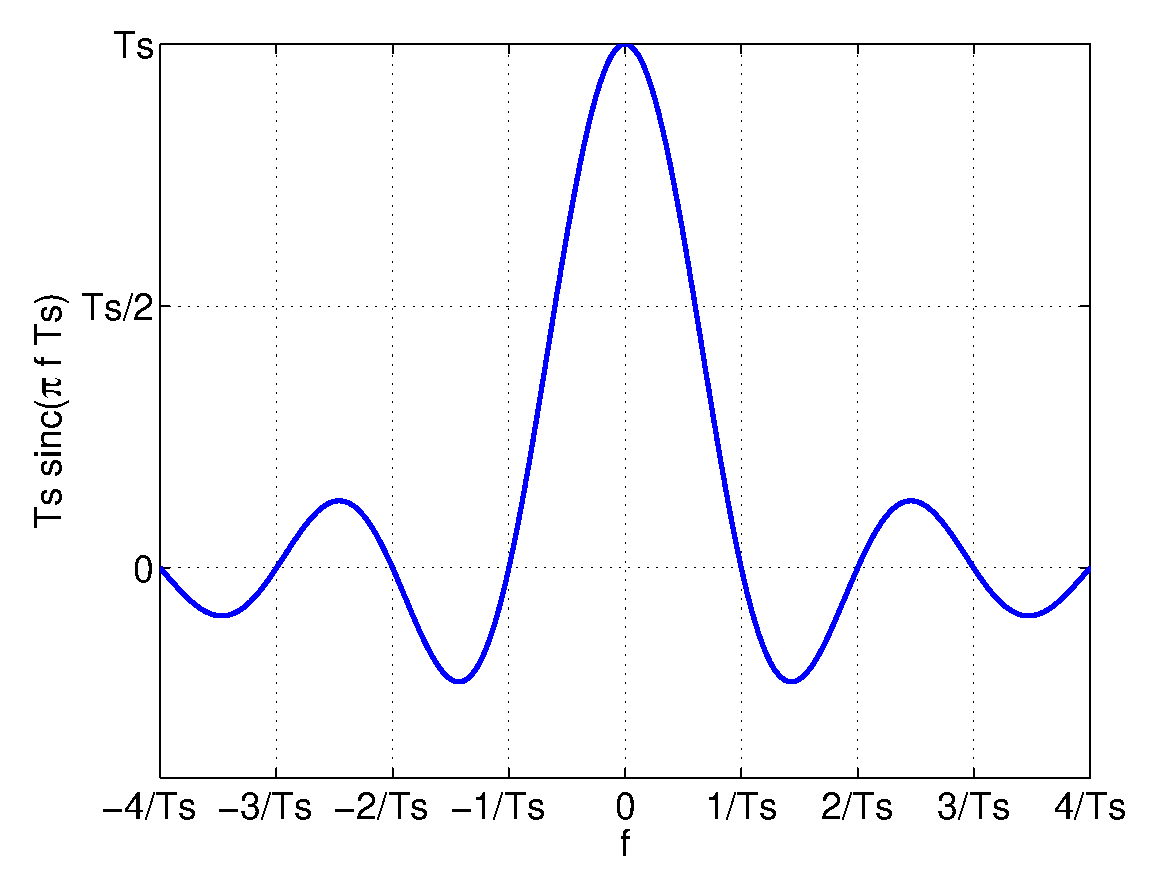
\includegraphics[width=0.45\textwidth]{../images/plotSinc.eps}(b)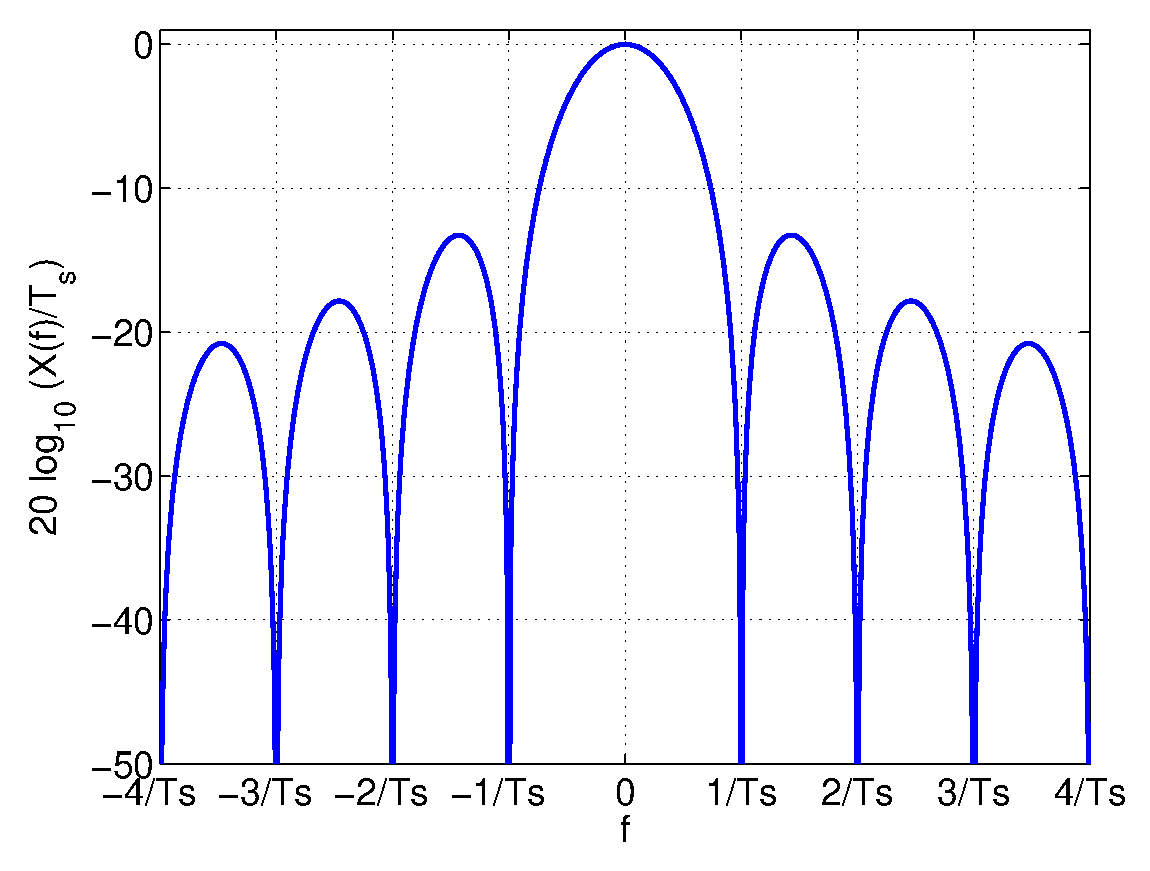
\includegraphics[width=0.45\textwidth]{../images/plotSincPowerdB.eps}
  \caption{(a) Fourier transform $X(j2\pi f)$ of rect pulse with period $T_s$, and (b) Power vs.\ frequency $20\log_{10}(X(j2\pi f)/T_s)$.}
  \label{F:plotSinc}
\end{figure}


\Question  What if $Y(j\omega)$ was a rect function?  What would the
inverse Fourier transform $y(t)$ be?

One can see a problem of using waveforms that are rectangular-shaped in \emph{either} the time or frequency domains.  If 100\% limited in the time domain, then the signal spreads infinitely in frequency; if 100\% limited in the frequency domain, then the signal spreads out infinitely in time.

\subsection{Fourier Transform Properties}

See Table 2.4.3 in the Rice book.

Assume that $\Fourier{x(t)} = X(j\omega)$.  Important properties of the
Fourier transform:
\begin{enumerate}
  \item Time shift property:
     \[
       \Fourier{x(t-t_0)} = e^{-j\omega t_0} X(j\omega)
     \]
  \item Scaling property: for any real $a\neq 0$,
     \[
       \Fourier{x(at)} = \frac{1}{|a|} X \left( j\frac{\omega}{a}\right)
     \]
  \item Convolution property: if, additionally $y(t)$ has Fourier
  transform $X(j\omega)$,
     \[
       \Fourier{x(t) \star y(t)} = X(j\omega) \cdot Y(j\omega)
     \]
  \item Modulation property:
     \[
       \Fourier{x(t) cos(\omega_0 t)} = \frac{1}{2}X(\omega-\omega_0)+ \frac{1}{2}X(\omega + \omega_0)
     \]
  \item Duality property:
     \begin{eqnarray}
       x(j\omega) &=& \Fourier{X(-t)} \nonumber \\
       x(-j\omega) &=& \Fourier{X(t)} \nonumber
     \end{eqnarray}
     This says is that you can go backwards in a Fourier transform table -- Replace the $\omega$ with $t$ in the frequency column, and replace $t$ with $-\omega$ in the time-domain column.
  \item Parceval's theorem:  The energy calculated in the frequency
  domain is equal to the energy calculated in the time domain.
     \[
       \int_{t=-\infty}^\infty |x(t)|^2 dt = \int_{f=-\infty}^\infty |X(f)|^2  df = \frac{1}{2\pi}\int_{\omega=-\infty}^\infty |X(j\omega)|^2 d\omega
     \]
     So do whichever one is easiest!  Or, check your answer by doing
     both.
\end{enumerate}

\Example{Applying FT Properties} If $w(t)$ has the Fourier transform $W(j \omega)$, find $X(j \omega)$ for the following:  $x(t) = w(2t + 2)$.

\Solution{
Let $x(t) = z(2t)$ where $z(t) = w(t+2)$.  Then $Z(j \omega) = e^{j2\omega} W(j \omega)$.  Then $X(j \omega) = \frac{1}{2}Z\left( \frac{j \omega}{2} \right)$.  So plugging in the first result,
  \[
   X(j \omega) = \frac{1}{2} e^{j\omega} W\left( \frac{j \omega}{2} \right).
  \]
  Alternatively, let $x(t) = y(t+1)$ where $y(t) = w(2t)$.  Then $X(j \omega) = e^{j\omega} Y(j \omega)$.  Then $Y(j \omega) = \frac{1}{2}W\left( \frac{j \omega}{2} \right)$.  Plugging in,
  \[
   X(j \omega) = e^{j\omega} \frac{1}{2}W \left( \frac{j \omega}{2} \right).
  \]
  The two approaches come up with the same answer, as they should.
}



\subsection{Bandwidth}

Bandwidth is a critical resource for a digital communications system; we have various definitions to quantify it.  In short, it isn't easy to describe a signal in the frequency domain with a single number.  And, in the end, a system will be designed to meet a spectral mask required by the FCC or system standard.

Intuitively, bandwidth is the maximum extent of our signal's frequency domain characterization $X(f)$.  A baseband signal absolute bandwidth is often defined as the $W$ such that $X(f)=0$ for all $f$ except for the range $-W \le f \le W$.  Other definitions for bandwidth are 
\begin{itemize}
 \item 3-dB bandwidth: $B_{3dB}$ is the value of $f$ such that $|X(f)|^2 = |X(0)|^2/2$.
 \item 90\% bandwidth: $B_{90\%}$ is the narrowest range which captures 90\% of the energy in the signal:
\[
  \int_{-B_{90\%}}^{B_{90\%}} |X(f)|^2 df = 0.90 \intinfty{f}{|X(f)|^2}
\]
\end{itemize}

As a motivating example, I mention the square-root raised cosine (SRRC) pulse, which has the following desirable Fourier transform:
\begin{equation} \label{E:RRC}
H_{RRC}(f) = \pdfarrays{\sqrt{T_{s}}}{0 \le |f| \le
\frac{1-\alpha}{2T_{s}}}
                      {\sqrt{\frac{T_{s}}{2}\left\{ 1 + \cos \left[
                      \frac{\pi T_{s}}{\alpha} \left( |f| - \frac{1-\alpha}{2T_{s}}
                       \right)\right]\right\}}}{ \frac{1-\alpha}{2T_{s}} \le |f| \le
                       \frac{1+\alpha}{2T_{s}}}
\end{equation}
where $\alpha$ is a parameter called the ``rolloff factor''.  We can actually analyze this using the properties of the Fourier transform and many of the standard transforms you'll find in a Fourier transform table.

The SRRC and other pulse shapes are discussed in Appendix A, and we will go into more detail later on.  The purpose so far is to motivate practicing up on frequency transforms. 

\Example{Butterworth Filter} 
A Butterworth low-pass filter has a frequency response with magnitude,
\[
|H(f)| = \frac{1}{\sqrt{1 + (f/f_0)^{2n}}}
\]
where $n$ is the number of reactive components (\ie, inductors or
capacitors).
  \begin{enumerate}
    \item What is the 3dB bandwidth of this filter?
    \item Find the lowest $n$ so that $|H(f)|^2$ is constant to within 1
    dB over the frequency range $-0.8 f_0 < f < 0.8 f_0$.  Hint:
    $|H(f)|^2$ is strictly decreasing as $|f|$ increases.  So the requirement
    is that $|H(0)|^2$ is no more than 1.26 times $|H(0.8 f_0)|^2$.
  \end{enumerate}

\Solution{  
\begin{enumerate}
    \item The squared magnitude, $|H(f)|^2$ is equal to 1/2 when $f=f_0$, regardless of $n$.  Thus the 3dB bandwidth is always $f_0$.
    \item  $|H(f)|$ is strictly decreasing from $f=0$.  We need to find the
      $n$ such that $|H(\pm 0.8 f_0)|^2$ is more than 1 dB down from
      the filter's maximum value (at $f=0$).  Note that
      \[
        10 \log_{10} |H(f)|^2 = -10 \log_{10} \left( 1 + (f/f_0)^{2n}\right)
      \]
      which makes $10 \log_{10} |H(0)|^2 = 0$ and thus we are looking for the $n$ that
      has:
      \begin{eqnarray}
        -1 &=& 10 \log_{10} |H(0.8 f_0)|^2 = - 10 \log_{10}(1+0.8^{2n})
          \nonumber \\
       0.1 &=& \log_{10} (1+0.8^{2n})
          \nonumber \\
       10^{0.1} - 1 &=& 0.8^{2n}
          \nonumber \\
       n &=& \frac{ \log(10^{0.1} - 1)}{2 \log(0.8)} \approx 3.03
          \nonumber
      \end{eqnarray}
      While $n=3$ is a good engineering answer, $n=4$ is a good math answer, since $n=3$, technically, would lead to $> 1$ dB variation.
  \end{enumerate}
}


\subsection{Linear Time Invariant (LTI) Filters}

If a (deterministic) signal $x(t)$ is input to a LTI filter with
impulse response $h(t)$, the output signal is
\[
  y(t) = h(t) \star x(t)
\]
Using the above convolution property,
\[
  Y(j \omega) = X(j \omega)  H(j \omega)
\]

\section{Sampling}

A common statement of the Nyquist sampling theorem is that a signal
can be sampled at twice its bandwidth.  But the theorem really has
to do with signal reconstruction from a sampled signal.

\Theorem{(Nyquist Sampling Theorem.) Let $x_c(t)$ be a baseband,
continuous signal with bandwidth $B$ (in Hz), \ie, $X_c(j\omega) = 0$ for
all $|\omega| \ge 2\pi B$. Let $x_c(t)$ be sampled at multiples of
$T$, where $\frac{1}{T} \ge 2B$ to yield the sequence
$\{x_c(nT) \}_{n=-\infty}^\infty $. Then
\begin{equation} \label{E:NyquistSamplingTheorem}
  x_c(t) = 2BT \sum_{n=-\infty}^\infty x_c(nT)
  \frac{\sin (2\pi B(t-nT))}{2\pi B(t-nT)}.
\end{equation}}
{Not covered.}

Notes:
\begin{itemize}
\item This is an interpolation procedure.
\item This is a synthesis equation with $\frac{\sin (2\pi B(t-nT))}{2\pi B(t-nT)}$ waveforms as the orthogonal basis functions.
\item This is only precise when $X(j\omega) = 0$ for all $|\omega| \ge 2\pi B$.
\end{itemize}

\subsection{Aliasing Due To Sampling}

Essentially, sampling is the multiplication of a impulse train (at
period $T$ with the desired signal $x(t)$:
\begin{eqnarray} \label{E:SampledViaImpulseTrain}
  x_{sa}(t) &=&  x(t) \sum_{n=-\infty}^\infty \delta(t-nT) \nnn
  x_{sa}(t) &=&  \sum_{n=-\infty}^\infty x(nT)  \delta(t-nT) \nn
\end{eqnarray}

What is the Fourier transform of $x_{sa}(t)$?  In the frequency domain, this is a convolution:
\begin{eqnarray} \label{E:FT_of_Sampled_Signal_1}
  X_{sa}(j\omega) &=& X(j\omega) \star \frac{2\pi}{T} \sum_{n=-\infty}^\infty \delta\left(\omega- \frac{2\pi n}{T} \right)
    \nonumber \\
  &=& \frac{1}{T}  \sum_{n=-\infty}^\infty X\left(j \left( \omega- \frac{2\pi n}{T}
  \right) \right) \quad \mbox{for all } \omega
    \\
  &=& \frac{1}{T}  X(j\omega) \quad \mbox{for } |\omega| < 2\pi B \mbox{ if } X(j\omega) \mbox{is bandlimited.}
    \nonumber
\end{eqnarray}}

This is shown graphically in the Rice book in Section 2.6.1 ``The Sampling Theorem'', Figure 2.12.

The Fourier transform of the sampled signal is many copies of $X(j\omega)$
strung at integer multiples of $2\pi /T$, as shown in
Fig.~\ref{F:Sampling-FreqDomain}.

\begin{figure}[htbp]
  \centerline{ 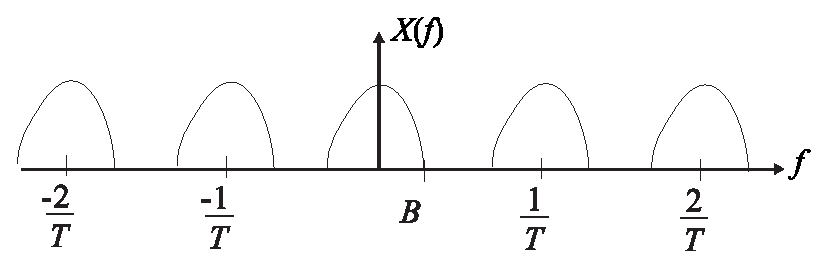
\includegraphics[width=0.65\textwidth]{../images/Sampling-FreqDomain_bandwidthB_f.eps}}
  \caption{The effect of sampling on the frequency spectrum in terms of frequency $f$ in Hz.}
  \label{F:Sampling-FreqDomain}
\end{figure}

\Example{Sinusoid sampled above and below Nyquist rate} Consider two
sinusoidal signals sampled at $1/T = 25$ Hz:
\begin{eqnarray}
  x_1(nT) &=& \sin(2 \pi 5 n T) \nnn
  x_2(nT) &=& \sin(2 \pi 20 n T) \nn
\end{eqnarray}
What are the two frequencies of the sinusoids, and what is the
Nyquist rate?  Which of them does the Nyquist theorem apply to? Draw
the spectrums of the continuous signals $x_1(t)$ and $x_2(t)$, and
indicate what the spectrum is of the sampled signals.

Figure \ref{F:NyquistInterpolations_SinusoidalSignals} shows what
happens when the Nyquist theorem is applied to the each signal
(whether or not it is valid).  What observations would you make
about Figure \ref{F:NyquistInterpolations_SinusoidalSignals}(b),
compared to Figure
\ref{F:NyquistInterpolations_SinusoidalSignals}(a)?

\begin{figure}[htbp]
  (a)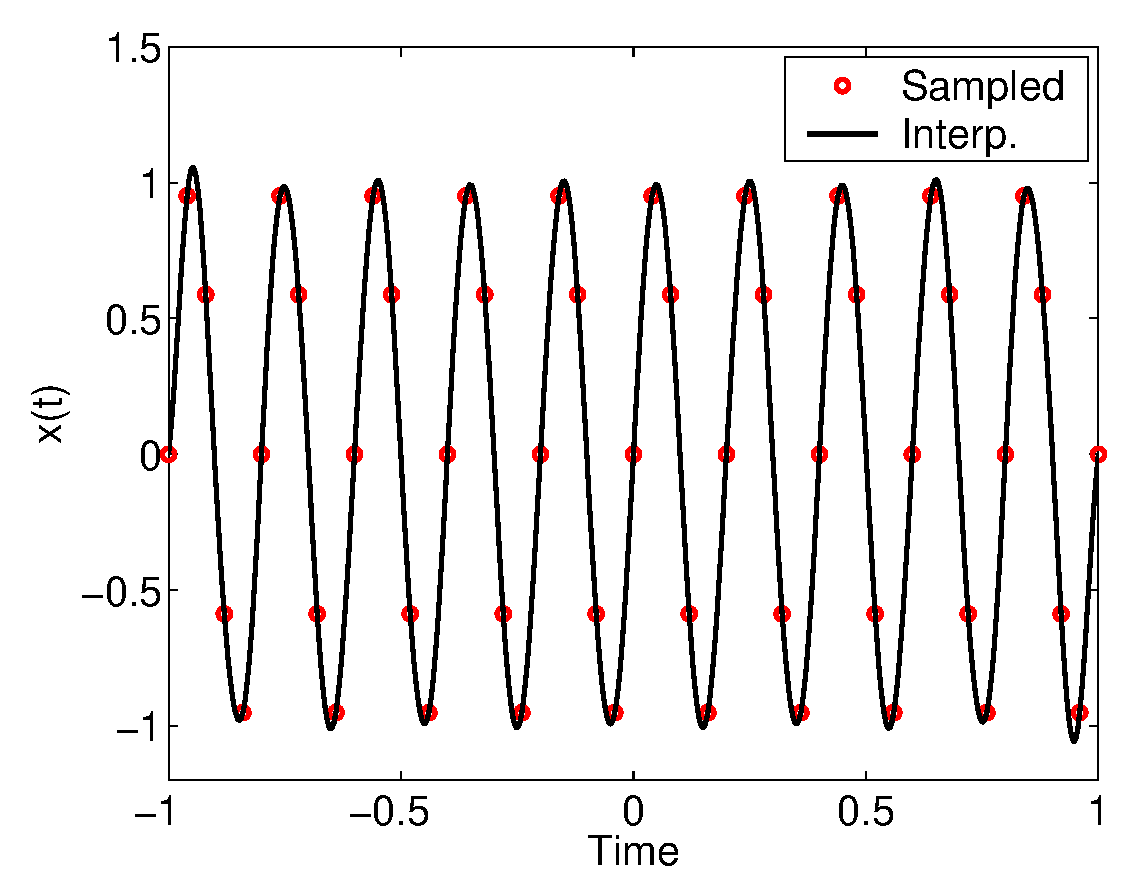
\includegraphics[width=0.45\textwidth]{../images/plotInterpolatedSin_f5.eps}(b)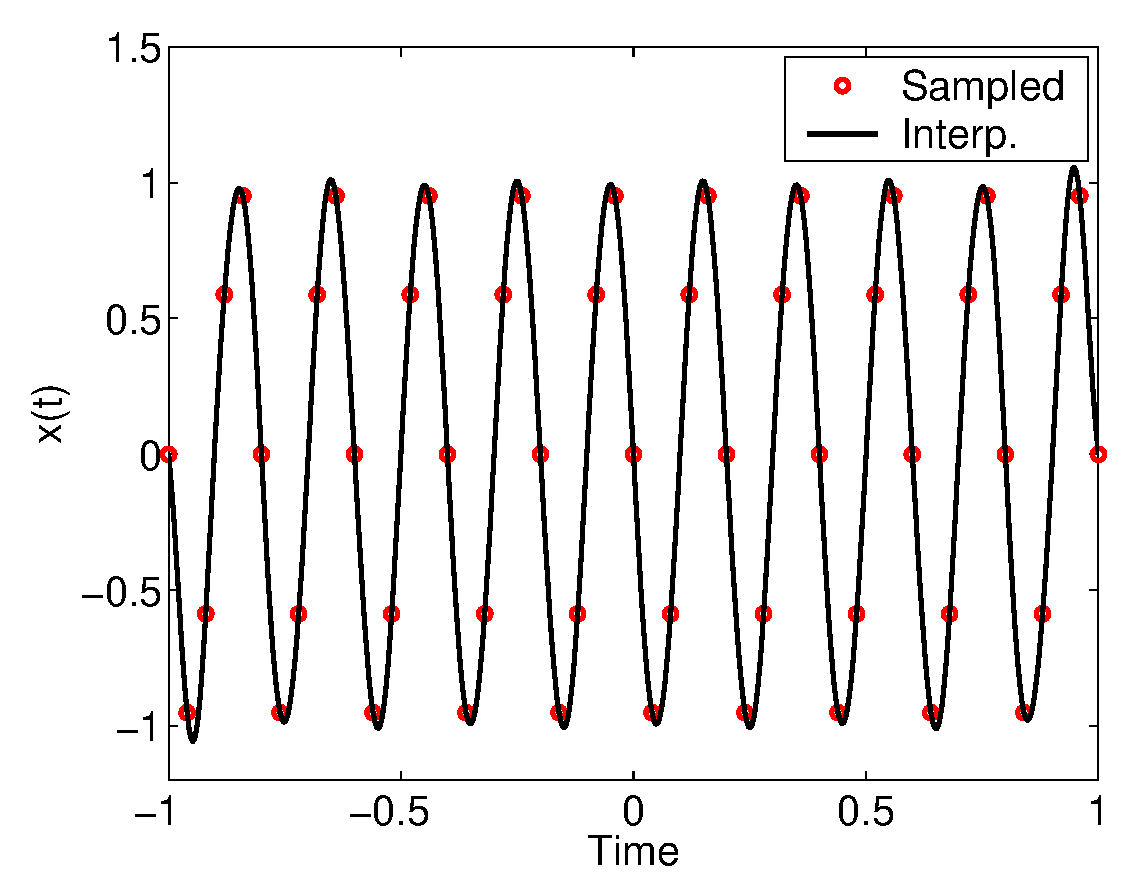
\includegraphics[width=0.45\textwidth]{../images/plotInterpolatedSin_f20.eps}
  \caption{Sampled (a) $x_1(nT)$ and (b) $x_2(nT)$ are interpolated (---) using the Nyquist interpolation formula.}
  \label{F:NyquistInterpolations_SinusoidalSignals}
\end{figure}


\Example{Square vs.\ round pulse shape} Consider the square pulse
considered before, $x_1(t) = \rect(t/T_s)$.  Also consider a
parabola pulse (this doesn't really exist in the wild -- I'm making it up for an example.)
\[
  x_2(t) = \pdfarray{1- \left(\frac{2t}{T_s}\right)^2}
                    {-\frac{1}{2T_s} \le t \le \frac{1}{2T_s}}
\]
What happens to $x_1(t)$ and $x_2(t)$ when they are sampled at rate
$T$?

\begin{figure}[htbp]
  (a)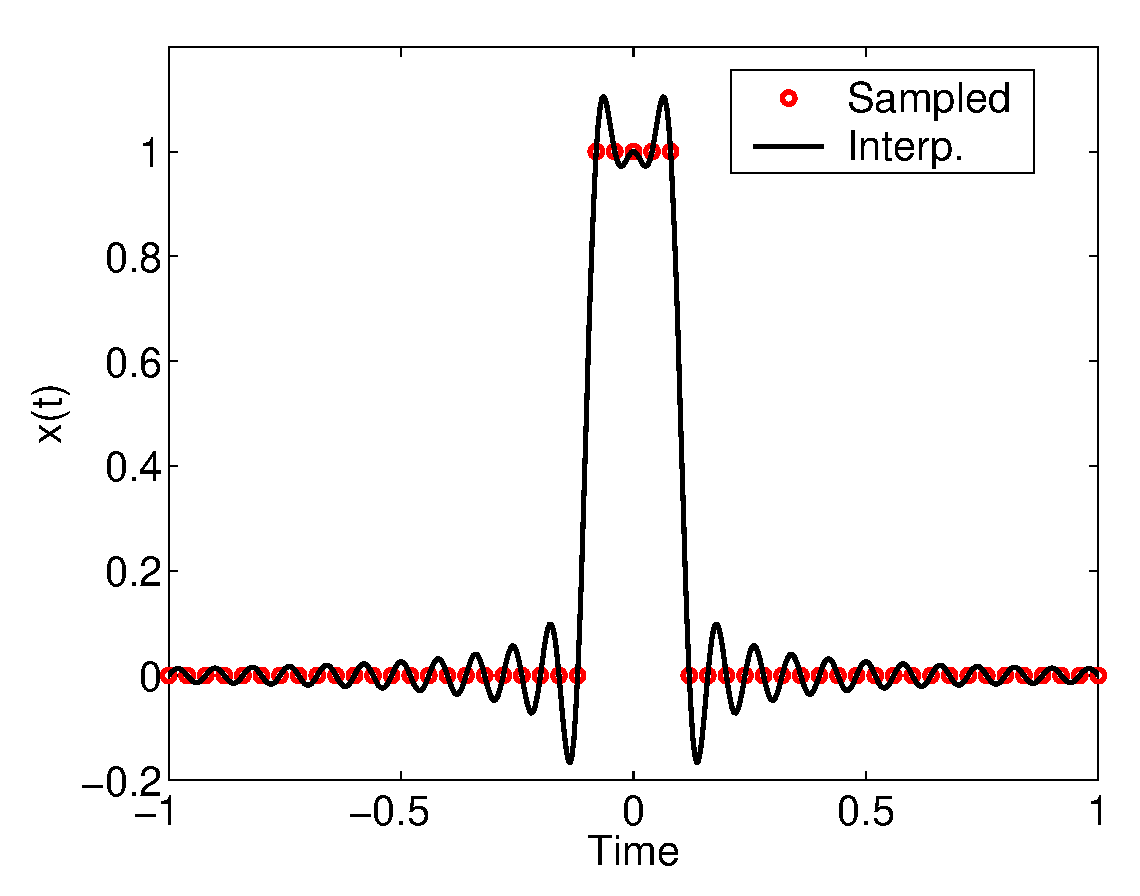
\includegraphics[width=0.45\textwidth]{../images/plotEgNyquistInterpolation_SquarePulse.eps}(b)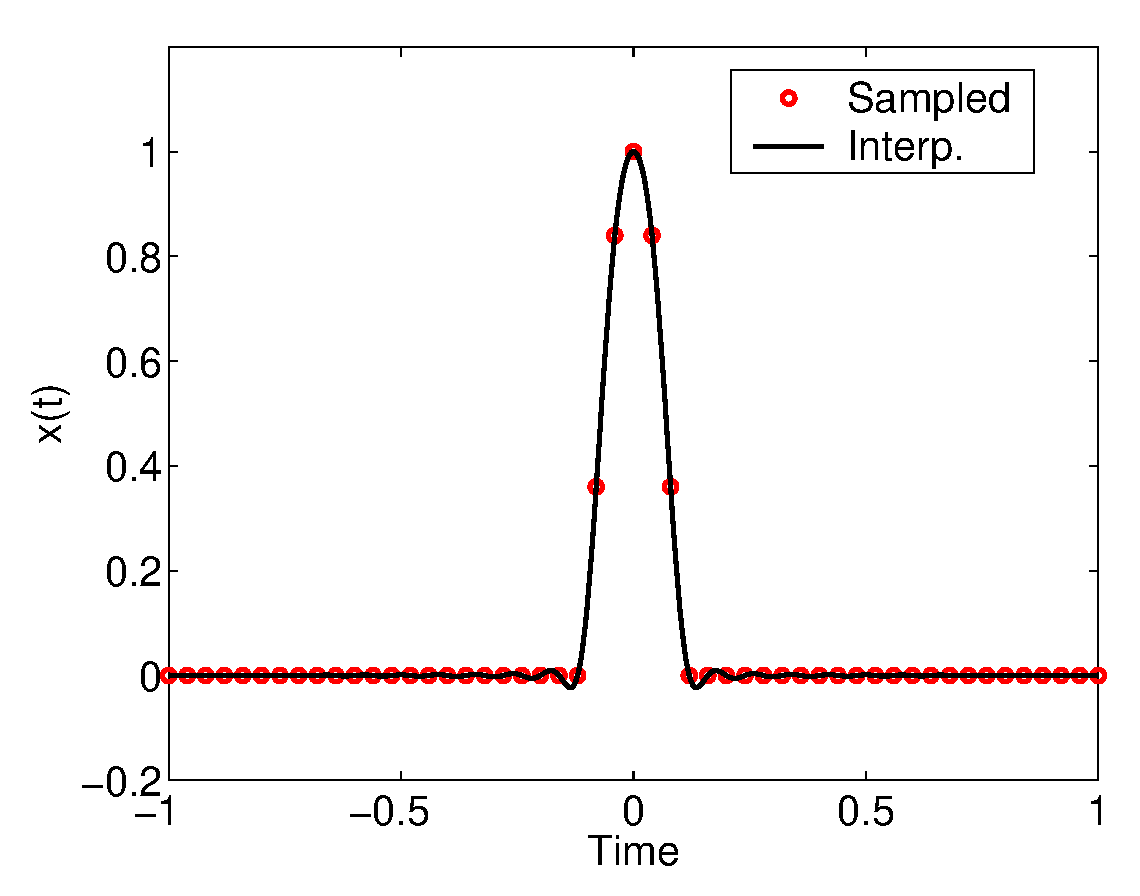
\includegraphics[width=0.5\textwidth]{../images/plotEgNyquistInterpolation_ParabolaPulse.eps}
  \caption{Sampled (a) $x_1(nT)$ and (b) $x_2(nT)$ are interpolated (---) using the Nyquist interpolation formula.}
  \label{F:NyquistInterpolations}
\end{figure}

In the Matlab code \texttt{EgNyquistInterpolation.m}  we set
$T_s=1/5$ and $T=1/25$.  Then, the sampled pulses are
interpolated using (\ref{E:NyquistSamplingTheorem}). Even though
we've sampled at a pretty high rate, the reconstructed signals will
not be perfect representations of the original, in particular for
$x_1(t)$.  See Figure \ref{F:NyquistInterpolations}.


% \subsection{Connection to DTFT}
% 
% Recall (\ref{E:SampledViaImpulseTrain}).  We calculated the Fourier
% transform of the product by doing the convolution in the frequency
% domain.  Instead, we can calculate it directly from the formula.
% 
% \begin{eqnarray} \label{E:FT_of_sampledSignal}
%   X_{sa}(j \omega) &=&  \int_{t=-\infty}^\infty \sum_{n=-\infty}^\infty x(nT)  \delta(t-nT) e^{-j\omega t}
%   \nnn
%     &=&  \sum_{n=-\infty}^\infty x(nT)  \int_{t=-\infty}^\infty  \delta(t-nT) e^{-j\omega t}
%   \\
%     &=&  \sum_{n=-\infty}^\infty x(nT)  e^{-j\omega n T}
%   \nn
% \end{eqnarray}
% 
% The discrete-time Fourier transform of $x_{sa}(t)$, I denote
% $\DTFT{x_{sa}(t)}$, and it is:
% \[
%  \DTFT{x_{sa}(t)} =  X_{d}(e^{j\Omega}) = \sum_{n=-\infty}^\infty x(nT)  e^{-j\Omega n}
% \]
% Essentially, the difference between the DTFT and the Fourier
% transform \emph{of the sampled signal} is the relationship
% \[
%  \Omega =  \omega T = 2\pi f T
% \]
% 
% But this defines the relationship only between the Fourier transform
% of the sampled signal.  How can we relate this to the FT of the
% continuous-time signal?  A: Using (\ref{E:FT_of_Sampled_Signal_1}). We
% have that $X_{d}(e^{j\omega}) = X_{sa}\left( \frac{\Omega}{T}\right)$.  Then plugging into (\ref{E:FT_of_Sampled_Signal_1}),
% \begin{eqnarray}
%   X_{d}(e^{j\Omega}) &=& X_{sa}\left( j \frac{\Omega}{T}\right)
%   \nnn
%    &=&  \frac{1}{T}  \sum_{n=-\infty}^\infty X\left(j \left( \frac{\Omega}{T} - \frac{2\pi n}{T}
%   \right) \right) \nnn
%    &=&  \frac{1}{T}  \sum_{n=-\infty}^\infty X\left(j \left( \frac{\Omega - 2\pi n}{T}
%   \right) \right) \nnn
% \end{eqnarray}
% 
% 
%  If $x(t)$ is sufficiently bandlimited, $X_{d}(e^{j\Omega}) \propto X(j\Omega/T)$
% in the interval $-\pi < \Omega < \pi$. This relationship holds for the Fourier transform of the original,
% \emph{continuous-time signal} between $-\pi < \Omega < \pi$
% \textbf{if and only if} the original signal $x(t)$ is sufficiently
% \textbf{bandlimited} so that the Nyquist sampling theorem applies.
% 
% 
% Notes:
% \begin{itemize}
%   \item Most things in the DTFT table in Table 2.4.8 are analogous to continuous functions which are not bandlimited.  So - don't expect the last form to apply to any continuous function.
%   \item The DTFT is periodic in $\Omega$ with period $2\pi$.
%   \item Don't be confused:  The DTFT is a continuous function of  $\Omega$.
% \end{itemize}
% 
% 
% 
% 

 


\StartOf{Lecture 5}

\Today{(0) Sampling from L4, (1) Intro to PAM, (2) ISI / Nyquist Filtering Theorem}

\announcements{
\begin{itemize}
  \item Today:  Rice A.2, 3.2.  For Wed: Rice 5.2, 5.3
  \item HW 2 due Thursday 11:59pm (extended one day).  Late deadline of Friday 11:59pm.
  \item Project 1 due Monday a week from today at 11:59pm. First 4 projects have been postponed by one week.
  \item Office hours: Mon 2:30-4pm, Tue 11-noon at Kaldi's coffee (Skinker and Forest Park Parkway)
  \item Keren Li (our AI) will have office hours weekly, Wed 4-5pm, location t.b.a.
\end{itemize}
}

\section{Intro to PAM}

Pulse amplitude modulation is a one-dimensional modulation, that is, it has one waveform $\phi_0(t)$.  We write this as $\phi_0(t) = p(t)$, where $p(t)$ is a unit-energy waveform called the pulse shape.  (The reason to use $p(t)$ will become clear later when we introduce other modulations.)  To encode symbols, we will choose an amplitude $a_{m,0}$ to indicate the $m$th symbol, and make the $a_{m,0}$ different.  For example, for $M=2$, we might choose amplitudes $\{-A, A\}$ (this is also called binary bipolar PAM).  The variable $A$ then determines the energy of the symbol.  As another example, for $M=4$, we could choose from the set $\{-3A, -A, A, 3A\}$.  These are equally spaced, but for $M> 2$, different symbols have different energies.  In particular, for $M$-PAM, the constellation diagram is shown in Rice Section 5.2.1, %Figure 5.2.1 (??), 
and amplitudes $\{a_{m,0}\}_m$ are,
\[
 -(M-1)A, -(M-3)A, \ldots, -A, A, \ldots, (M-3)A, (M-1)A
\]
The average energy, assuming that each symbol is equally likely, can be shown to be:
\[
 E_{avg} = \frac{M^2-1}{3}A^2
\]

To send multiple symbols over time, we transmit a signal $s(t)$,
\[
 s(t) = \sum_n a(n) p(t-nT_s),
\]
where $a(n)$ is the amplitude (one of the $\{a_{m,0}\}_m$) of the $n$th symbol we choose to send, and $T_s$ is the symbol period.  Each subsequent pulse is delayed in time by $T_s$.  


\Example{Binary Bipolar PAM} Figure \ref{F:PAM-binary-square-pulse}
shows a 4-ary PAM signal set using amplitudes $a_{0,0}=-A$, $a_{1,0} = A$.
It shows a signal set using square pulses,
\[
  \phi_0(t) = p(t) = \pdfarray{1/\sqrt{T_{s}}}{0 \le t < T_{s}}
\]
  \begin{figure}[htbp]
    \centerline{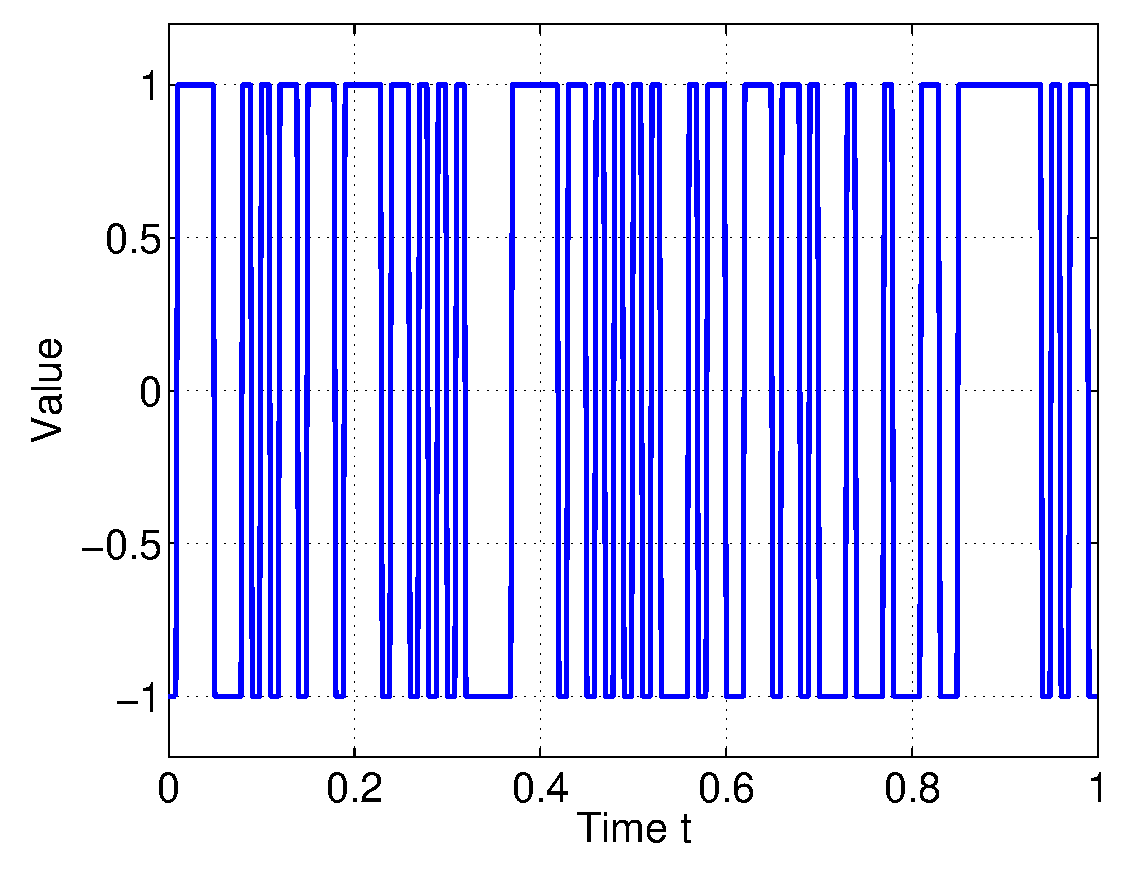
\includegraphics[width=0.6\textwidth]{../images/PAM-binary-square-pulse.eps} }
    \caption{Example signal for binary bipolar PAM example for $A = \sqrt{T_{s}}$.}
    \label{F:PAM-binary-square-pulse}
  \end{figure}


At the receiver, what we do is multiply the received signal $r(t)$ by $\phi_0(t)$ and integrate:
\[
 x = \int_{t=-\infty}^\infty r(t) \phi_0(t) dt
\]
This is also called \emph{correlation}. This needs to happen at each multiple of $T_s$. 
But there really are finite limits -- let's say that the signal has
a duration $T_s$, and then rewrite the integral as
\begin{equation} \label{E:Correlation}
 x = \int_{t=0}^{T_s} r(t) \phi_0(t) dt
\end{equation}
Essentially, this is as if we had multiple orthogonal waveforms, and thus our receiver is a bunch of parallel correlations, each time delayed by $T_s$, as shown in Figure \ref{F:multiple_correlation}.  Note that my integral limits in Figure \ref{F:multiple_correlation} may be wider if the pulse is wider than $T_s$ (e.g., the $n$th branch would start before $nT_s$ and end after $(n+1)T_s$).

  \begin{figure}[htbp]
    \centerline{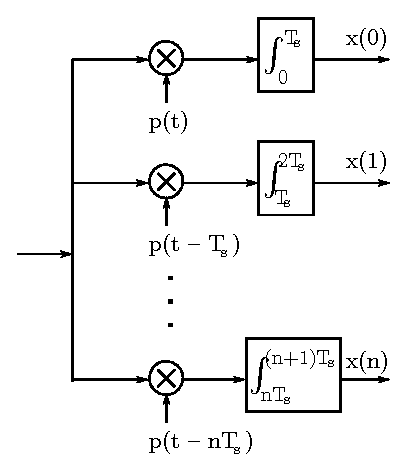
\includegraphics[width=0.5\textwidth]{../images/time_delay_correlation_receiver.eps} }
    \caption{The pulse shape $p(t)$ is chosen to be orthogonal to itself at integer multiples of the time delay.  Thus a PAM receiver might be implemented as a correlation receiver, in which each correlation (multiplication and integration) is done in parallel.}
    \label{F:multiple_correlation}
  \end{figure}
  
In reality, instead of a correlation, we can equivalently do a matched filter.  Equation (\ref{E:Correlation}) can be written as
\[
 x = \int_{t=0}^{T_s} r(t) h(T_s - t) dt
\]
where $h(t) = \phi_0(T_s-t)$.  (Plug in $(T_s-t)$ in this formula and
the $T_s$s cancel out and only positive $t$ is left.)  This is the
output of a convolution, taken at time $T_s$,
\[
 x =  \left. r(t) \star h(t) \right|_{t=T_s}
\]
Or equivalently
\[
 x =  \left. r(t) \star \phi_0(T_s-t) \right|_{t=T_s}
\]

  \begin{figure}[htbp]
    \centerline{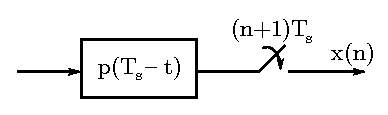
\includegraphics[width=0.45\textwidth]{../images/matched_filter_receiver.eps} }
    \caption{A matched filter receiver inputs $r(t)$ to a filter with impulse response $p(T_s-t)$, and then samples the output each multiple of $T_s$.}
    \label{F:matched_filter_rx}
  \end{figure}

Notes:
\begin{itemize}
  \item $x(n)$ is the output of a matched filter at time $nT_s$.
  \item We might, for example, have a physical filter with the impulse
    response $\phi_0(T_s-t)$, in which case it would be easy to do a matched filter
    implementation.
\end{itemize}

Try out the Matlab code,
\texttt{correlation\_and\_matched\_filter\_rx.m}, which is posted on
Canvas, for some examples of a pulse shape, adding noise, and performing the filtering for a correlation and matched filter receiver.


\section{Inter-Symbol Interference (ISI)}


\begin{enumerate}
  \item Consider the spectrum of the ideal 1-D PAM system with a square pulse.
  \item Consider the time-domain of the signal which is close to a rect function in the frequency domain.
\end{enumerate}
We don't want either:  (1) the pulse occupies too much spectrum, and (2) the pluse occupies too much time.
\begin{enumerate}
  \item If we try (1) above and use FDMA (frequency division
  multiple access) then the interference is \emph{out-of-band
  interference}.
  \item If we try (2) above and put symbols right next to each other in time, our
  own symbols experience interference called \emph{inter-symbol
  interference}.
\end{enumerate}

In reality, we want to compromise between (1) and (2) and experience
only a small amount of both.




\subsection{Nyquist Filtering}

We want to extend the pulse $p(t)$ to be longer in duration than only between zero and $T_s$, but we want to do so in a way that preserves the property that $p(t)$ and $p(t-T_s)$, and for that matter, $p(t-nT_s)$ for integers $n\neq 0$, are orthogonal.

Key insight:  we don't need $p(t)$ and $p(t-\tau)$ to be orthogonal for all real-valued times $\tau$ -- only for $\tau = nT_{s}$, for integer $n$.  In other words, the set:
\[
 \ldots,p(t+2T_s), p(t+T_s), p(t), p(t-T_s), p(t-2T_s), \ldots
\]
form an orthonormal set.  The Nyquist filtering condition is a frequency-domain rule that can be used to design arbitrary pulse shapes $p(t)$ that meet this condition.


\Theorem{Nyquist Filtering}{Let $r_p(t) = \intinfty{\tau}{p(\tau)p(\tau-t)}$ be the autocorrelation function of pulse shape $p(t)$.  A necessary and sufficient condition for
$r_p(t)$ to satisfy
\[
  r_p(nT_{s}) = \pdfarray{1}{n=0}
\]
is that its Fourier transform $R_p(f)$ satisfy
\[
  \sum_{m=-\infty}^\infty R_p\left(f + \frac{m}{T_{s}}\right) = T_{s}
\]
}{Proof: on page 677, Appendix A, of Rice book.}

Basically, $R_p(f)$ could be:
\begin{itemize}
  \item $R_p(f) = \rect(fT_{s})$, \ie, exactly constant within $-\frac{1}{2T_{s}} < f < \frac{1}{2T_{s}}$ band
  and zero outside.
  \item It may bleed into the next `channel' but the sum of
    \[ \cdots + R_p\left(f - \frac{1}{T_{s}}\right) + R_p(f) +
          R_p\left(f + \frac{1}{T_{s}}\right) + \cdots \]
    must be constant across all $f$.
\end{itemize}
Thus $R_p(f)$ is allowed to bleed into other frequency bands -- but
the neighboring frequency-shifted copy of $R_p(f)$ must be lower s.t.
the sum is constant.  See Figure \ref{F:NyquistFiltering}.

\begin{figure}[htbp]
\centerline{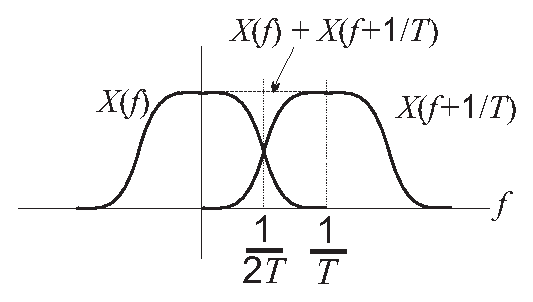
\includegraphics[width=0.7\textwidth]{../images/NyquistFiltering.eps}}
\caption{The Nyquist filtering criterion --
$1/T_{s}$-frequency-shifted copies of $R_p(f)$ must add up to a
constant.}\label{F:NyquistFiltering}
\end{figure}

If $R_p(f)$ only bleeds into one neighboring channel (that is, $R_p(f) =
0$ for all $|f| > \frac{1}{T_{s}}$), we denote the difference
between the ideal rect function and our $R_p(f)$ as $\Delta(f)$,
\[
  \Delta(f) = \left| R_p(f) - \rect(fT_{s}) \right|
\]
then we can rewrite the Nyquist Filtering condition as,
\[
   \Delta\left( \frac{1}{2T_{s}} - f \right) = \Delta\left( \frac{1}{2T_{s}} + f \right)
\]
for $-1/T_{s} \le f < 1/T_{s}$.  Essentially, symmetric about
$f=1/(2T_{s})$. See Figure \ref{F:NyquistFiltering}

Bateman presents this whole condition as ``A Nyquist channel
response is characterized by the transfer function having a
transition band that is symmetrical about a frequency equal to $0.5
\times 1/T_{s}$.''

\vspace{0.1in} \noindent {\bf Activity:}  Do-it-yourself Nyquist filter.  Take a sheet of paper and fold it in half, and then in half the other direction.  Cut a function in the thickest side (the edge that you just folded).  Leave a tiny bit so that it is not completely disconnected into two halves.  Unfold.  Drawing a horizontal line for the frequency $f$  axis, the middle is $0.5/T_s$, and the vertical axis it $R_p(f)$. One half (bottom or top) will be a plot of $R_p(f)$, and the other half will be an (inverse) plot of $R_p(f-T_s)$.


\subsection{Square Root Raised Cosine Pulse Shapes}

The raised-cosine function is given by:
\begin{equation} \label{E:RC}
H_{RC}(f) = \pdfarrays{T_{s}}{0 \le |f| \le
\frac{1-\alpha}{2T_{s}}}
                      {\frac{T_{s}}{2}\left\{ 1 + \cos \left[
                      \frac{\pi T_{s}}{\alpha} \left( |f| - \frac{1-\alpha}{2T_{s}}
                       \right)\right]\right\}}{ \frac{1-\alpha}{2T_{s}} \le |f| \le
                       \frac{1+\alpha}{2T_{s}}}
\end{equation}
Note that this is the $R_p(f)= H_{RC}(f)$ that meets the Nyquist filtering condition.  The pulse shape $p(t)$ must be such that $r_p(t)$, the autocorrelation function, has the Fourier transform $R_p(t)$.  How do we get that?  Well, recall that convolution in the time domain is multiplication in the frequency domain.  And autocorrelation (correlation with the same function itself) then is squaring in the frequency domain.  Thus $r_p(t) = \intinfty{\tau}{p(\tau)p(\tau-t)}$ means that $R_p(f) = |P(f)|^2$ or $|R_p(f)|^{1/2} = |P(f)|$.  For the RC $R_p(f)$ function, this leads to a ``square root'' raised cosine (SRRC) pulse shape.

\begin{equation} \label{E:SRRC}
H_{RRC}(f) = \pdfarrays{\sqrt{T_{s}}}{0 \le |f| \le
\frac{1-\alpha}{2T_{s}}}
                      {\sqrt{\frac{T_{s}}{2}\left\{ 1 + \cos \left[
                      \frac{\pi T_{s}}{\alpha} \left( |f| - \frac{1-\alpha}{2T_{s}}
                       \right)\right]\right\}}}{ \frac{1-\alpha}{2T_{s}} \le |f| \le
                       \frac{1+\alpha}{2T_{s}}}
\end{equation}


\begin{figure}[htbp]
  \centerline{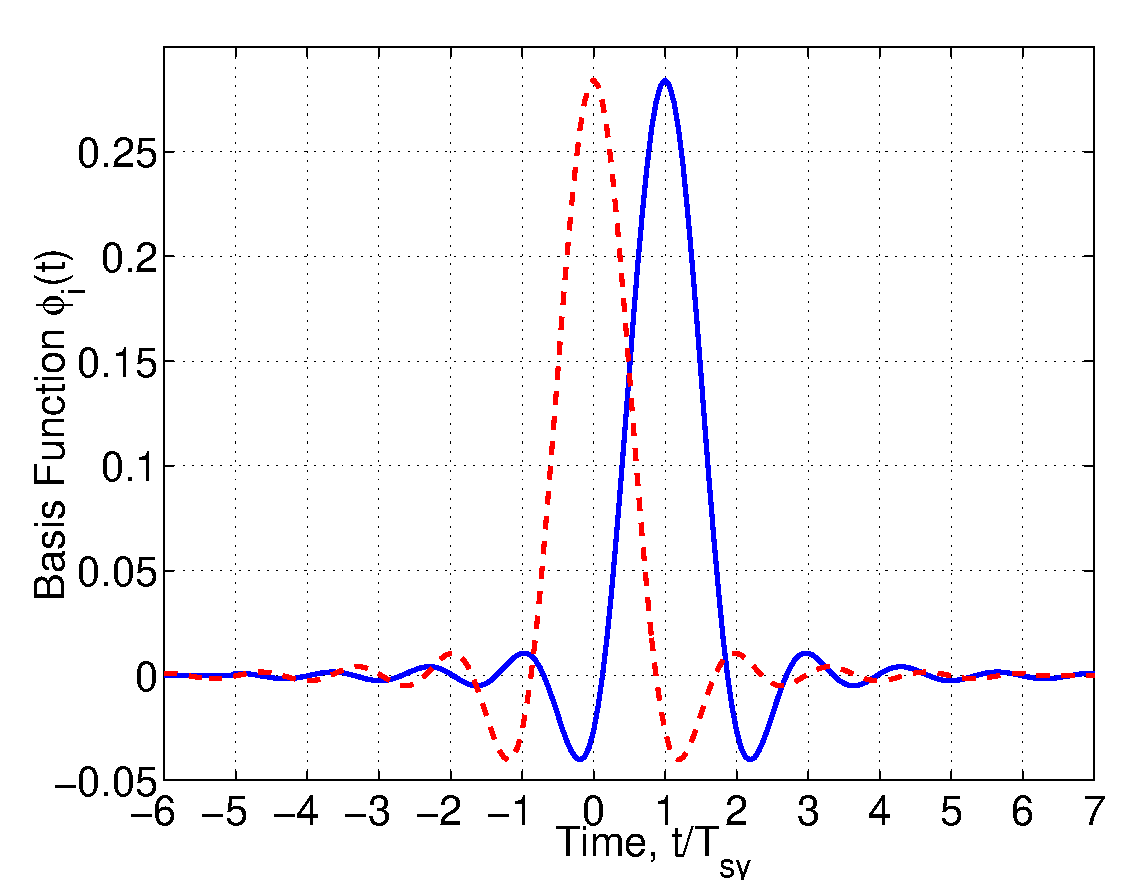
\includegraphics[width=0.6\textwidth]{../images/plotTwoTimeDelayedSRRCPulses.eps}}
  \caption{Two SRRC Pulses, delayed in time by $nT_{s}$ for any integer $n$, are orthogonal to each other.}
  \label{F:plotTwoTimeDelayedSRRCPulses}
\end{figure}


 


\StartOf{Lecture 6}

\Today{(0) Nyquist Filtering, (1) QAM, (2) PSK}

\announcements{
\begin{itemize}
  \item For today: Rice Chapter 5.2, 5.3
  \item For Mon:  Proakis \& Salehi FSK sections (From page 4 ''Frequency-Shift Keying (FSK)'' through Equation (7.5.90) on page 10 of the pdf). See Canvas.  And:  Rice 5.4. 
  \item HW 2 due tomorrow (Thu) 11:59pm. 
  \item Proj.\ 1 due Mon 11:59pm.  
  \item HW 3 posted, due Wed.\ Feb.\ 12.  
  \item Keren Li has office hours today 4-5pm in the Green Hall 2120A conference room.
\end{itemize}
}

\section{Quadrature Amplitude Modulation (QAM)}

Quadrature Amplitude Modulation (QAM) is a two-dimensional
bandpass signalling method which uses the in-phase and quadrature (cosine and sine, respectively) as the two dimensions.  Thus QAM uses two basis functions.  These are:
\begin{eqnarray} \label{E:QAM_basis}
  \phi_0(t) &=& \sqrt{2} p(t) \cos(\omega_0 t) \nnn
  \phi_1(t) &=& - \sqrt{2} p(t) \sin(\omega_0 t) 
\end{eqnarray}
where $p(t)$ is a pulse shape (like the ones we've looked at
previously) with support on $T_1 \le t \le T_2$.  That is, $p(t)$ is
only non-zero within that window.

In most flow chart-type drawings of transmitters and receivers, frequency up-conversion and down-conversion are separate from pulse shaping, which is largely true to how the device operates.  The definition of the orthonormal basis in (\ref{E:QAM_basis}) specifically considers a pulse shape at a frequency $\omega_0$.  We include it here because it is \emph{critical} to see how, with the same pulse shape $p(t)$, we can have two orthogonal basis functions.  (This is not intuitive!)

We have two restrictions on $p(t)$ that makes these two basis
functions orthonormal:
\begin{itemize}
  \item $p(t)$ is unit-energy.
  \item $p(t)$ is `low pass'; that is, it has low frequency content
  compared to $\omega_0 t$.
\end{itemize}

\subsection{Showing Orthogonality}

Let's show that the basis functions are orthogonal.  Rather than assume that the waveforms are infinite in duration, let's put finite limits $T_1$ and $T_2$ on them, and say that they are zero before $T_1$ and after $T_2$.  Starting the proof, and using $\sin (2 A) = 2 \cos A \sin A$,
\begin{eqnarray}
  \intinfty{t}{\phi_0(t)\phi_1(t)}  &=&
    - \int_{T_1}^{T_2} \sqrt{2} p(t) \cos(\omega_0 t) \sqrt{2} p(t) \sin(\omega_0
    t) dt \nnn
    &=& - 2 \int_{T_1}^{T_2} p^2(t) \cos(\omega_0 t) \sin(\omega_0 t) dt \nnn
    &=& - \int_{T_1}^{T_2} p^2(t) \sin(2 \omega_0 t) dt. \nn
\end{eqnarray}

But we don't know $p(t)$, so we can't proceed.  For a simple example, let $p(t)=c$ for a constant $c$ , for $T_1 \le t \le T_2$.  Are the two bases orthogonal?
\begin{eqnarray} \label{E:constant_pulse_mid}
  \intinfty{t}{\phi_0(t)\phi_1(t)}
    &=&  - c^2 \int_{T_1}^{T_2}  \sin(2 \omega_0 t) dt \nnn
    &=&  - c^2 \left[  - \frac{\cos(2 \omega_0 t)}{2\omega_0} \right|_{T_1}^{T_2} \nnn
    &=&  - c^2 \frac{\cos(2 \omega_0 T_2) - \cos(2 \omega_0 T_1)}{2\omega_0} 
\end{eqnarray}
Next, using the relationship,
\begin{equation}
  \cos A - \cos B = -2\sin  \frac{A + B}{2}  \sin \frac{A - B}{2}, 
\end{equation}
we can write (\ref{E:constant_pulse_mid}) as,
\begin{eqnarray}
 \intinfty{t}{\phi_0(t)\phi_1(t)} 
    &=&  c^2 \frac{\sin(\omega_0 (T_2+T_1)) \sin(\omega_0 (T_2-T_1))}{\omega_0}
    \nn
\end{eqnarray}
We only need one of the sinusoids to be zero to make the functions orthogonal.  There are two cases:
\begin{enumerate}
  \item The pulse duration $T_2-T_1$ is an integer number of
  periods.  That is, $\omega_0 (T_2-T_1) = \pi k$ for some integer
  $k$.  In this case, the right $\sin$ is zero, and so the
  correlation is exactly zero.
  \item Otherwise, the numerator bounded above and below by +1 and
  -1, because it is a sinusoid.  That is,
  \[
    -\frac{c^2}{\omega_0} \le \langle \phi_0(t), \phi_1(t) \rangle \le \frac{c^2}{\omega_0}
  \]
  Typically, $\omega_0$ is a large number.  For example, frequencies $2\pi \omega_0$ could be
  in the MHz or GHz ranges.  Certainly, when we divide by numbers on the order of $10^6$ or
  $10^9$, we're going to get a very small inner product.  For
  engineering purposes, then, $\phi_0(t)$ and $\phi_1(t)$ are orthogonal.
\end{enumerate}

Finally, we can attempt the proof for the case of arbitrary pulse
shape $p(t)$.  In this case, we use the `low-pass' assumption that
the maximum frequency content of $p(t)$ is much lower than $2\pi
\omega_0$.  This assumption allows us to assume that $p^2(t)$ is
nearly constant over the course of one cycle of the carrier
sinusoid.

This is well-illustrated in Figure 5.3.1 in the Rice book (page 240).
In this figure, we see a pulse modulated by a sine wave at frequency
$2\pi\omega_0$.  Zooming in on any few cycles, you can see that the
pulse $p^2(t)$ is largely constant across each cycle.  Thus, when we
integrate $p^2(t) \sin(2 \omega_0 t)$ across one cycle, we're going
to end up with approximately zero. 

%\Solution{How many cycles are there?  Consider the period $[T_1,T_2]$.  How many times can it be divided by $\pi /\omega_0$?  Letthe integer number be
%\[
%  L = \left\lfloor \frac{(T_2-T_1)\omega_0}{\pi } \right\rfloor.
%\]
%Then each cycle is in the period, $[ T_1 + (i-1)\pi/\omega_0 , T_1 + i\pi/\omega_0 ]$, for $i=1, \ldots, L$.  Within each of these cycles, assume $p^2(t)$ is nearly constant.  Then, in the same way that the earlier integral was zero, this part of the integral is zero here. The only remainder is the remainder (partial cycle) period, $[T_1 + L\pi/\omega_0 , T_2]$. Thus
%\begin{eqnarray}
%  \langle \phi_0(t), \phi_1(t) \rangle
%    &=& p^2(T_1+L\pi/\omega_0) \int_{T_1+L\pi/\omega_0}^{T_2} \sin(2 \omega_0 t) dt
%    \nnn
%    &=& p^2(T_1+L\pi/\omega_0)\frac{\cos(2 \omega_0 T_2) - \cos(2 \omega_0 T_1 + 2\pi L)}{2\omega_0}
%    \nnn
%    &=& p^2(T_1+L\pi/\omega_0)\frac{\sin(\omega_0 (T_2+T_1)) \sin(\omega_0 (T_2-T_1))}{\omega_0}
%    \nn
%\end{eqnarray}
 %}
%Again, the inner product is bounded on either side:
%\[
%  -\frac{p^2(T_1+L\pi/\omega_0)}{\omega_0} \le \langle \phi_0(t), \phi_1(t)
%  \rangle \frac{p^2(T_1+L\pi/\omega_0)}{\omega_0}
%\]
%which for very large $\omega_0$, is nearly zero.

\subsection{Constellation}

With these two basis functions, $M$-ary QAM is defined as an
arbitrary signal set $\mba_0, \ldots, \mba_{M-1}$, where each signal
space vector $\mba_k$ is two-dimensional:
\[
  \mba_k = [a_{k,0}, a_{k,1}]^T
\]

The signal corresponding to symbol $k$ in ($M$-ary) QAM is thus
\begin{eqnarray}
 s(t) &=& a_{k,0}  \phi_0( t) + a_{k,1} \phi_1( t) \nnn
   &=& a_{k,0}  \sqrt{2} p(t) \cos(\omega_0 t) - a_{k,1} \sqrt{2} p(t) \sin(\omega_0
 t) \nnn
   &=& \sqrt{2} p(t)  \left[ a_{k,0}  \cos(\omega_0 t) - a_{k,1} \sin(\omega_0 t) \right] \nn
\end{eqnarray} Note that we could also write the signal $s(t)$ as
\begin{eqnarray}
 s(t) &=& \sqrt{2} p(t)  \mathbb{Re} \left\{ a_{k,0} e^{j\omega_0 t} + j a_{k,1} e^{j\omega_0 t} \right\} \nnn
  &=& \sqrt{2} p(t)  \mathbb{Re} \left\{ e^{j\omega_0 t} \left( a_{k,0} + j a_{k,1}\right) \right\} \nnn
\end{eqnarray}
In many textbooks, you will see them write a QAM signal in shorthand
as
\[
 s_{CB}(t) = p(t) (a_{k,0} + j a_{k,1})
\]
This is called `Complex Baseband'.  If you do the following
operation you can recover the real signal $s(t)$ as
\[
 s(t) = \sqrt{2} \mathbb{Re} \left\{ e^{j\omega_0 t} s_{SB}(t) \right\}
\]
Many other books use complex baseband notation, so I include this because you
should be able to read other books and know what they're talking
about.

Then, we can see that the signal space representation $\mba_k$ is
given by
\[
  \mba_k = [a_{k,0}, a_{k,1}]^T
\]
for $k = 0,\ldots, M-1$

\subsection{Signal Constellations}

\begin{figure}[htbp]
  \centerline{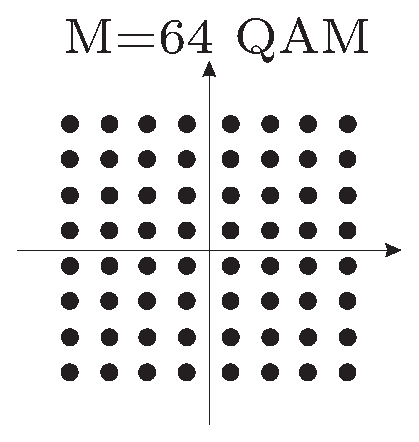
\includegraphics[width=0.3\textwidth]{../images/QAM64Eg.eps} }
  \caption{Square signal constellation for 64-QAM.}
  \label{F:QAM64Eg}
\end{figure}

\begin{itemize}
  \item See Figure 5.3.3 in the Rice book for examples of square QAM.  These
  constellations use $M = 2^{a}$ for some \textbf{even} integer $a$, and arrange
  the points in a grid.  One such diagram for $M=64$ square QAM is also given here in
  Figure \ref{F:QAM64Eg}.
  \item Figure 5.3.4 shows examples of constellations which use $M = 2^{a}$ for some \textbf{odd} integer $a$, and arrange the points in a grid.  These are either rectangular grids, or 
  squares with the corners cut out, or more hexagonal grids.
\end{itemize}

\subsection{Angle and Magnitude Representation}

You can plot $\mba_k$ in signal space and see that it has a
magnitude (distance from the origin) of $| \mba_k| = \sqrt{a_{k,0}^2
+ a_{k,1}^2}$ and angle of $\angle \mba_k =
\tan^{-1}\frac{a_{k,1}}{a_{k,0}}$.  In the continuous time signal
$s(t)$ this is
\[
s(t) = \sqrt{2} p(t) | \mba_k |  \cos(\omega_0 t + \angle \mba_k)
\]

\subsection{Average Energy in M-QAM}

The average energy is calculated as:
\begin{eqnarray}
  \En_s &=& \frac{1}{M} \sum_{i=0}^{M-1} |\mba_i|^2 \nnn
  \En_b &=& \frac{1}{M \log_2 M} \sum_{i=0}^{M-1} |\mba_i|^2 \nn
\end{eqnarray}
where $\En_s$ is the average energy per symbol and $\En_b$ is the
average energy per bit.  We'll work in class some examples of
finding $\En_b$ in different constellation diagrams.



\subsection{Phase-Shift Keying}

Some implementations of QAM limit the constellation to include only
signal space vectors with equal magnitude, \ie,
\[
  |\mba_0| = |\mba_1| = \cdots = |\mba_{M-1}|
\]
The points $\mba_i$ for $i=0, \ldots, M-1$ are uniformly spaced on
the unit circle.  Some examples are shown in Figure \ref{F:MPSKEg}.

\FigureFromAnotherLecture{
  \begin{figure}[htbp]
    \centerline{(a)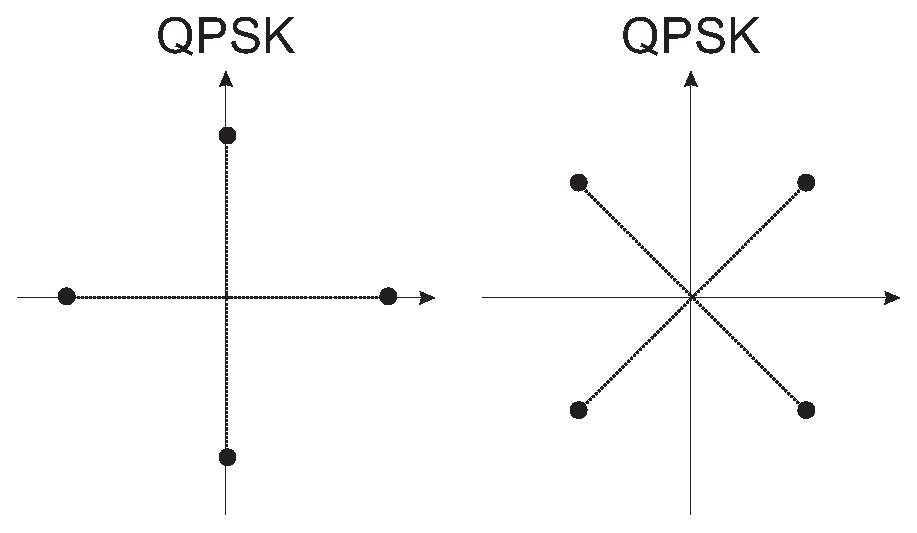
\includegraphics[width=0.6\textwidth]{../images/QPSK-signalSpaceDiagram.eps}
    }
    \centerline{(b)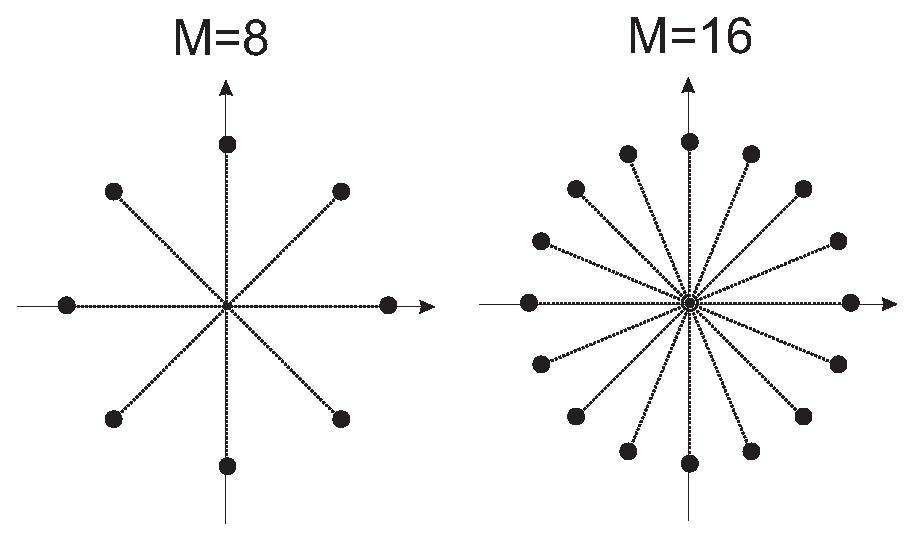
\includegraphics[width=0.6\textwidth]{../images/MPSK-signalSpaceDiagram.eps} }
    \caption{Signal constellations for (a) $M=4$ PSK and (b) $M=8$ and $M=16$ PSK.}
    \label{F:MPSKEg}
  \end{figure}
}

\paragraph{BPSK}

For example, binary phase-shift keying (BPSK) is the case of $M=2$.
Thus BPSK is the same as bipolar (2-ary) PAM.   What is the
probability of error in BPSK?  The same as in bipolar PAM, \ie, for
equally probable symbols,
\[
    \PR{\mbox{error}} = \Q{ \sqrt{\frac{2\En_b }{N_0}}}.
\]

\paragraph{QPSK}

$M=4$ PSK is also called quadrature phase shift keying (QPSK), and
is shown in Figure \ref{F:MPSKEg}(a).  Note that the rotation of the
signal space diagram doesn't matter, so both `versions' are
identical in concept (although would be a slightly different
implementation).  Note how QPSK is the same as $M=4$ square QAM.

\subsection{Systems which use QAM}

See L.W.~Couch, \emph{Digital and Analog Communication Systems}, 7th ed., 2007. Also: Wikipedia, and the Rice book:
\begin{itemize}
  \item Digital Microwave Relay, various manufacturer-specific
    protocols.  6 GHz, and 11 GHz.
  \item Dial-up modems: use a $M=16$ or $M=8$ QAM constellation.
  \item DSL.  G.DMT uses multicarrier (up to 256 carriers) methods (OFDM), and on each narrowband
    (4.3kHz) carrier, it can send up to $2^{15}$ QAM (32,768 QAM).
    G.Lite uses up to 128 carriers, each with up to $2^8=256$ QAM.
  \item Cable modems.  Upstream:  6 MHz bandwidth channel, with 64
    QAM or 256 QAM.  Downstream:  QPSK or 16 QAM.
  \item 802.11a, 802.11g:  Adaptive modulation methods, use up to 64 QAM.
  \item 802.11ac, 11ax: uses up to 1024 QAM.
  \item Digital Video Broadcast (DVB): APSK used in ETSI standard.
\end{itemize}


\subsection{Bandwidth of QAM, PAM, PSK}

The bandwidth of QAM, PAM, and PSK are all determined by the bandwidth of the pulse used.  For square root-raised cosine (SRRC) pulses, the null to null bandwidth is 
\[
 B_T = \frac{1+\alpha}{T_s}
\]
where $\alpha$ is the ``rolloff'' factor or ``excess bandwidth'' parameter of the SRRC pulse.  Recall if $\alpha=0$ then the pulse shape is a rect in the frequency domain and a sinc in the time domain, and has the smallest bandwidth.  



 


\StartOf{Lecture 7}

\Today{(0) Complex Baseband (1) OQPSK  (2) FSK}

\announcements{
\begin{itemize}
  \item For today: Proakis \& Salehi FSK section,   Rice 5.4, 5.5.
  \item Proj 1 due today.  HW 3 due Wed. Proj 2 due one week from today.  
  \item My Office hours: Today 2:30pm-4pm, Tue 11-noon. Keren Li office hour: Wed 4-5 (in Green Hall 2120A).
\end{itemize}
}

\subsection{Complex Baseband for QAM}

First, a short review.  Last lecture, we described QAM and PSK by their use of two basis functions at the same frequency $\omega_0$:
\begin{eqnarray}
  \phi_0(t) &=& \sqrt{2} p(t) \cos(\omega_0 t) \nnn
  \phi_1(t) &=& -\sqrt{2} p(t) \sin(\omega_0 t) \nn
\end{eqnarray}
We outlined the proof that these two are orthogonal.  We looked at some example symbol constellations and calculated their average symbol energies.  We showed that the bandwidth is a function of the pulse shape, for example, for SRRC pulse shapes, $B=(1+\alpha)/T_s$.

Our continuous-time signal will be a sequence of amplitude-scaled versions of these bases:
\begin{equation} \label{E:signal_QAM}
 s(t) = \sqrt{2} \sum_n \left[ a_0(n) p(t-nT_s) \cos(\omega_0 t) - a_1(n)  p(t-nT_s) \sin(\omega_0 t) \right],
\end{equation}
where $a_k(n)$ is the amplitude of $\phi_0$ used during the $n$th symbol period.  We often use $I(t)$, \ie, the in-phase component, as the part of the signal multiplying the $\cos(\omega_0 t)$, and $Q(t)$, \ie, the quadrature component, as the part of the signal multiplying the $\sin(\omega_0 t)$:
\begin{eqnarray}
 && I(t) = \sum_n a_0(n)p(t-nT_s), \quad Q(t) = \sum_n a_1(n)p(t-nT_s).\nnn
 && s(t) = \sqrt{2}  I(t) \cos(\omega_0 t)  - \sqrt{2}  Q(t) \sin(\omega_0 t). \nn
\end{eqnarray}
Alternatively, 
\begin{equation} \label{E:signal_Angle}
 s(t) = \sqrt{2} \sum_n \sqrt{a_0^2(n) + a_1^2(n)} p(t-nT_s) \cos\left(\omega_0 t + \tan^{-1} \frac{a_1(n)}{a_0(n)} \right) ,
\end{equation}
a form that shows that $s(t)$ during any symbol has an ``envelope'' or amplitude and a phase angle.  The envelope and angle are time-varying functions because the pulse amplitude is not constant.  

When we plot the in-phase vs. the quadrature, Rice calls it the ``phase trajectory plot''.  Actually, it shows the trajectory of both the phase and envelope.  An example for QPSK is shown in  Figure \ref{F:SimulationQPSK}.

\begin{figure}[htbp]
$\begin{array}{ll}
  (a)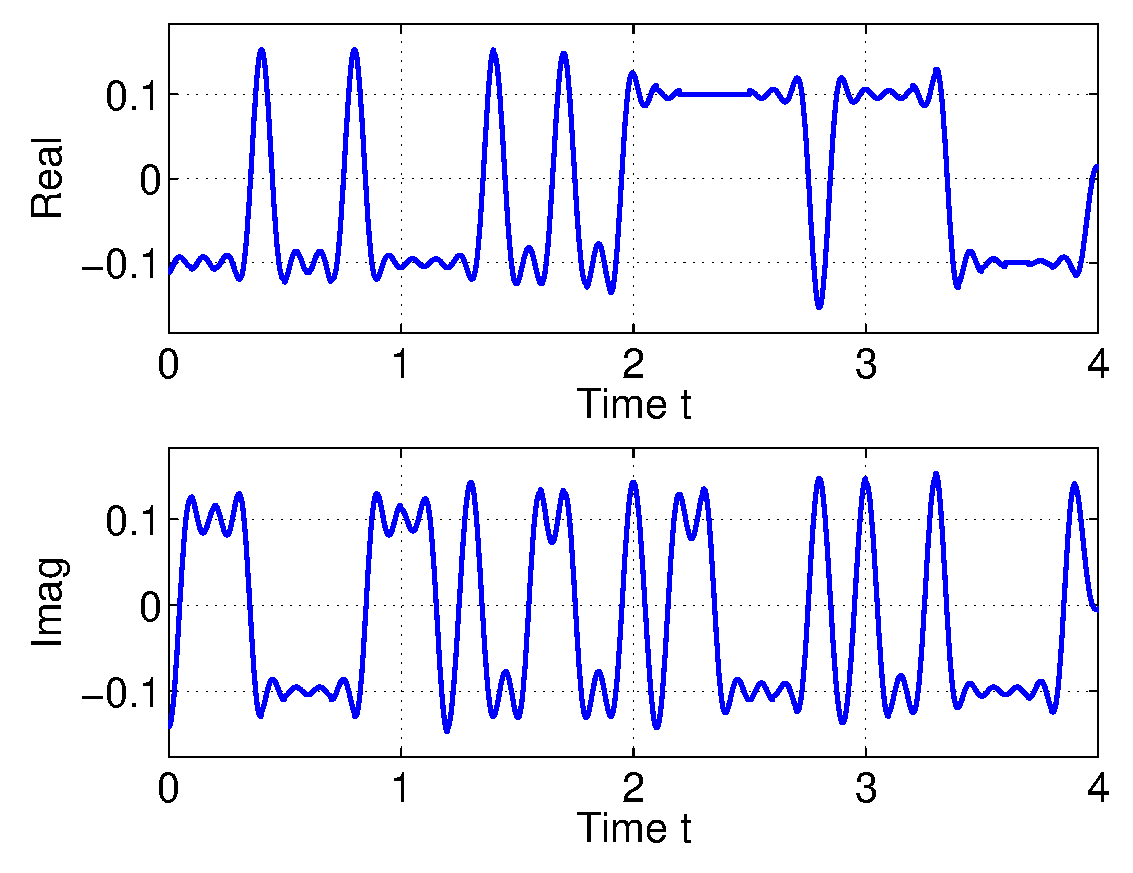
\includegraphics[width=0.45\textwidth]{../images/plotComplexSigQPSK.eps} &
  (b)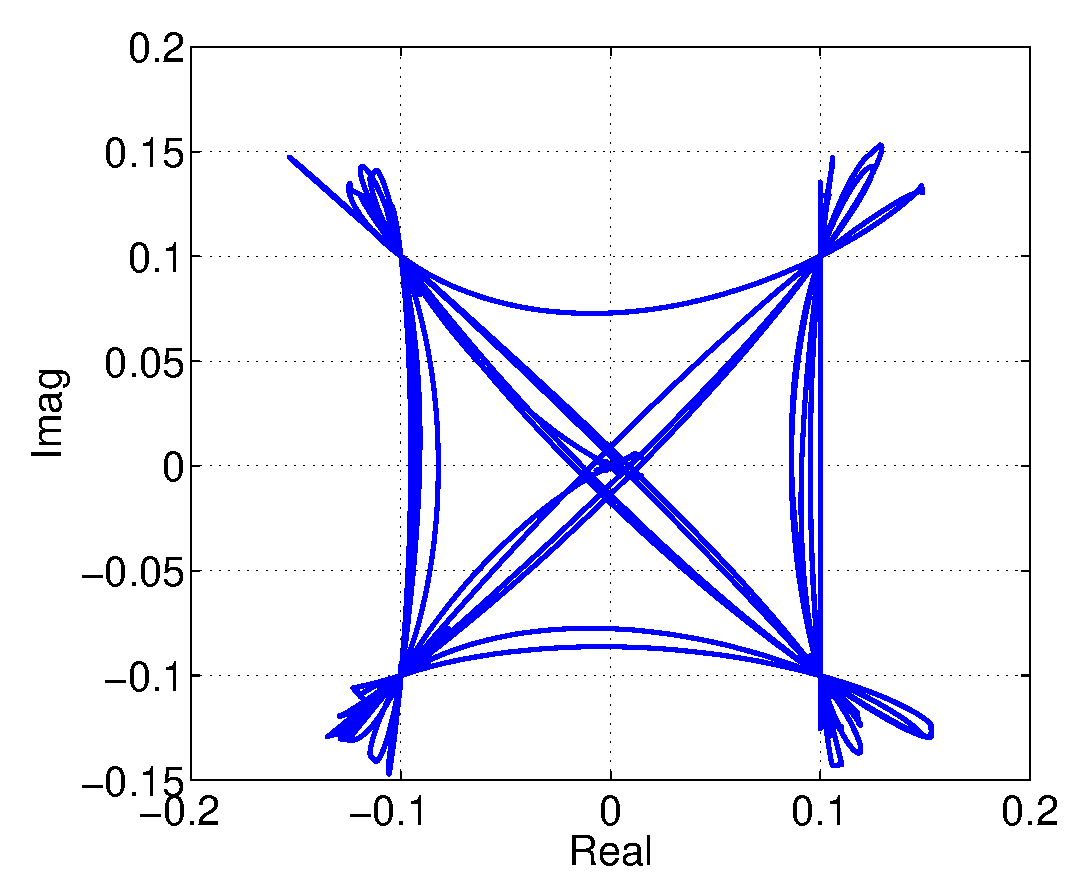
\includegraphics[width=0.45\textwidth]{../images/plotConstellationDiagramQPSK.eps}\\
  \end{array}$
  \caption{Matlab simulation of the complex baseband form of $s(t)$ for QPSK, showing the (a) in-phase (cosine) and quadrature (sine) components.  In the phase trajectory plot in (b), time is removed and we plot the in-phase vs.~the quadrature components.}
  \label{F:SimulationQPSK}
\end{figure}



\section{Offset QPSK (OQPSK)}

\subsection{Motivation}

One thing that makes a transmitter more power hungry is the need for a linear amplifier.  An amplifier uses DC power to take a bandpass input signal and increase its
amplitude at the output.  If $P_{DC}$ is the input power (\eg, from
battery) to the amplifier, and $P_{out}$ is the output signal power,
the power efficiency is rated as $\eta_P = P_{out} / P_{DC}$.

Truly linear amplifiers (class A) amplifiers are at most 50\% power efficient.  We are interested in the question, what signals can be amplified with nonlinear (class C) amplifiers that are around 90\% power efficient?  The answer is that ``constant envelope'' signals can.  These are signals that the peak envelope is never much higher than the average envelope.  The phase trajectory plot of a constant envelope signal will be nearly a circle, and it will never go through or near the origin (envelope of zero).

Not all modulations are constant envelope, so this involves some modulation limitations. In order to double the power efficiency, battery-powered transmitters are often willing to use constant envelope modulations so that they can use Class C amplifiers.  They can
do this if their output signal has constant envelope.  

\subsection{Definition}

The reason that QPSK is not constant envelope is that when the phase angle changes 180 degrees from one symbol to the next, the envelope will go through zero.  See Figure \ref{F:SimulationQPSK} to see this graphically.

Offset QPSK solves this problem by simply shifting one of the basis functions forward by half a symbol period, \ie, $T_s/2$.  The orthonormal basis for OQPSK are thus:
\begin{eqnarray}
  \phi_0(t) &=& \sqrt{2} p(t) \cos(\omega_0 t) \nnn
  \phi_1(t) &=& \sqrt{2} p(t - T_s/2) \sin(\omega_0 t) \nn
\end{eqnarray}
We still only offset subsequent symbols by $T_s$, so the transmitted signal is:
\[
 s(t) = \sqrt{2} \sum_n \left[ a_0(n) p(t-nT_s) \cos(\omega_0 t) + a_1(n)  p\left(t-\left(n+\frac{1}{2}\right)T_s\right) \sin(\omega_0 t) \right],
\]
or equivalently the in-phase and quadrature components are,
\[
 I(t) = \sqrt{2} \sum_n a_0(n)p(t-nT_s), \quad Q(t) = \sqrt{2} \sum_n a_1(n)p\left(t-\left(n+\frac{1}{2}\right)T_s\right).
\]
Compared to (\ref{E:signal_QAM}), the in-phase component of $s(t)$ in OQPSK does not go through zero at the same times that the quadrature component does, since the pulse functions $p()$ are offset in time by half a symbol period.  

Another way to look at this is to view the phase trajectory plot in Figure \ref{F:SimulationOQPSK}.  The signal never switches from its current constellation point to the one 180$^o$ opposite -- either the in-phase or quadrature component changes during any multiple of $T_s/2$, but NOT both.

\begin{figure}[htbp]
$\begin{array}{ll}
  (a)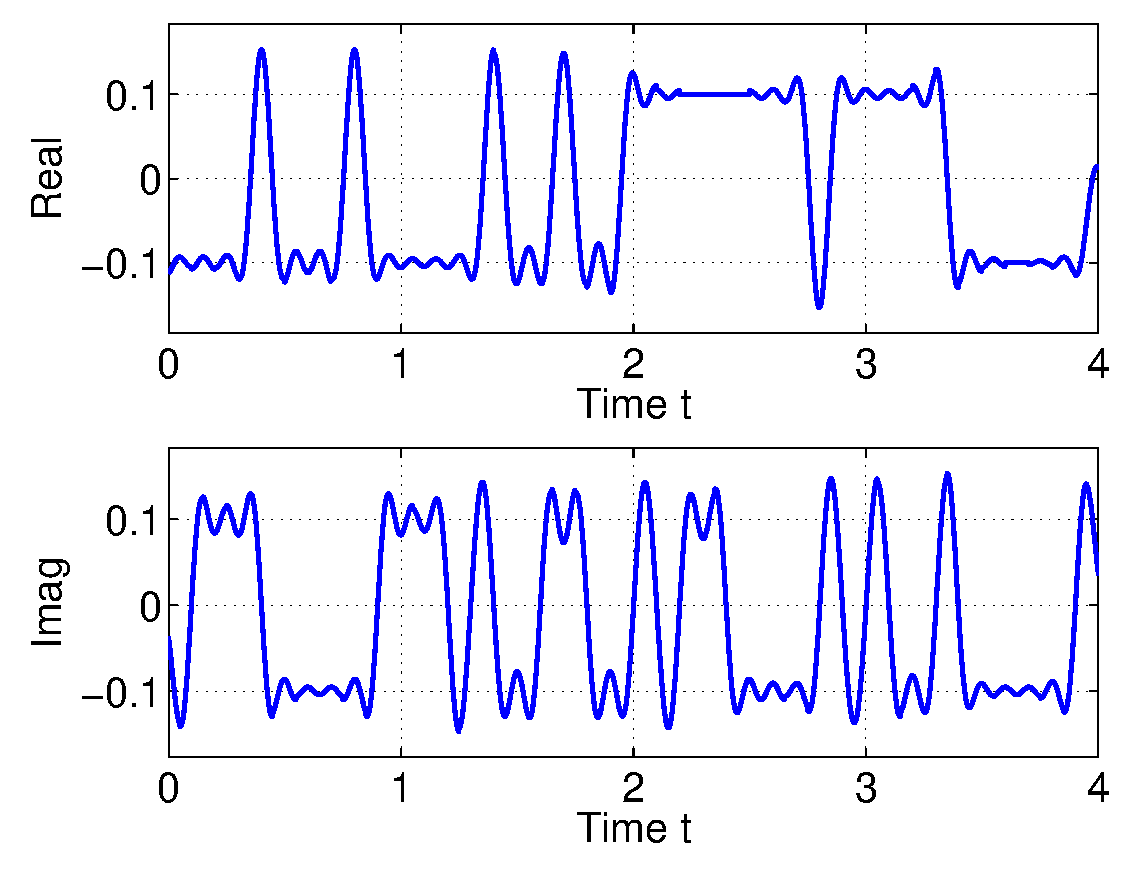
\includegraphics[width=0.45\textwidth]{../images/plotComplexSigOQPSK.eps} &
  (b)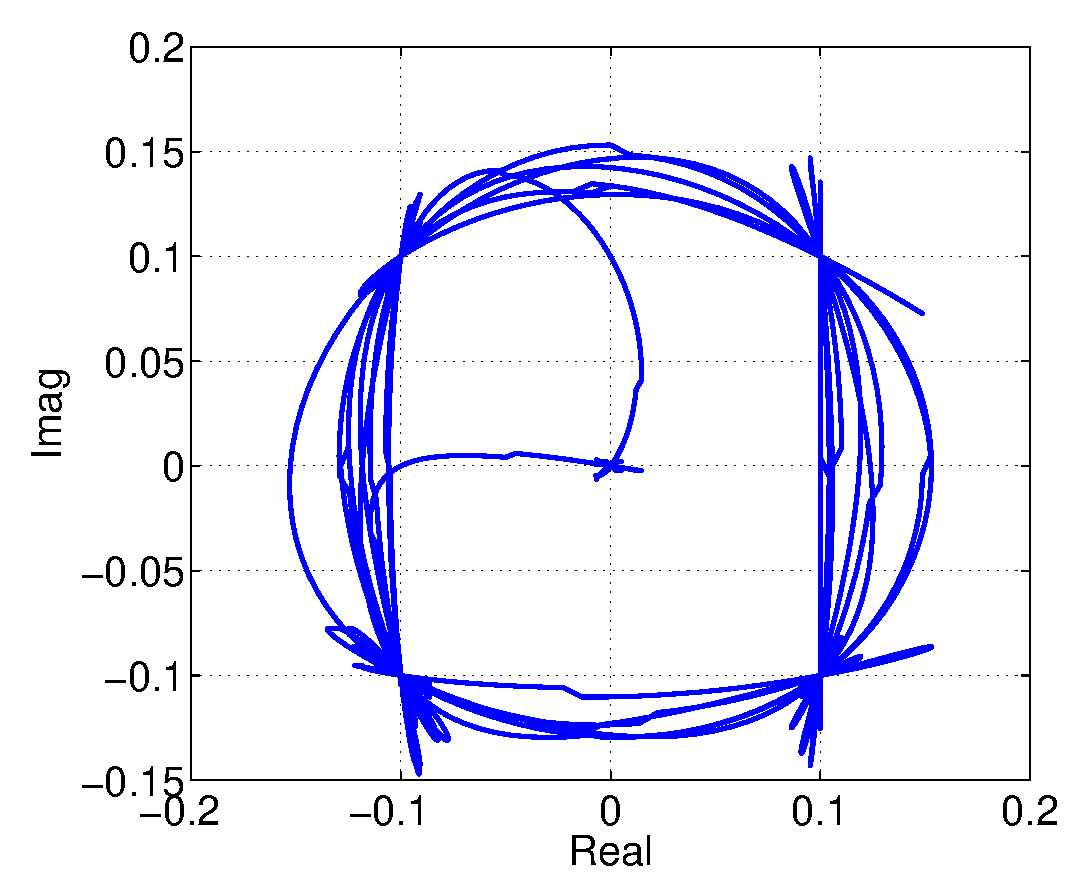
\includegraphics[width=0.45\textwidth]{../images/plotConstellationDiagramOQPSK.eps}
  \end{array}$
  \caption{Matlab simulation of $s(t)$ for OQPSK, showing the (a) in-phase (cosine) and quadrature (sine) components.  The phase trajectory plot in (b) shows the nearly constant envelope of OQPSK, compared to that for QPSK in Figure \ref{F:SimulationQPSK}.}
  \label{F:SimulationOQPSK}
\end{figure}


At the receiver, we just need to delay the sampling on the
in-phase component of the signal half of a sample period with respect to the quadrature
signal.  The new transmitted signal takes the same bandwidth and
average power, and as we will show later in the course, the same $E_b/N_0$ vs.~probability of bit
error performance.  However, the envelope $|s(t)|$ is largely
constant.  Compare Figures \ref{F:SimulationQPSK} and \ref{F:SimulationOQPSK} to see the differences between QPSK and OQPSK.

\section{Frequency Shift Keying (FSK)}

In frequency shift keying, symbols are selected to be sinusoids
with frequency selected among a set of $M$ different frequencies
$\{f_0, f_1, \ldots f_{M-1}\}$.  Note that in FSK, the number of basis functions equals the number of symbols.  Consider $f_{k} = f_c + k\Delta f$, and thus
\begin{equation} \label{E:FSK-Symbols4}
 \phi_k(t) = \sqrt{2} p(t) \cos(\omega_0 t + 2\pi k\Delta f t)
\end{equation}
where $p(t)$ is our pulse shape.  We want these $\phi_k(t)$ to form an orthonormal basis.  How can we make them orthonormal?  First, note that these basis functions are unit energy, just like we've shown that the QAM basis functions are unit energy.  Next, what do we get when we find the inner product of two different basis functions,  $\phi_k(t)$ and $\phi_m(t)$ for $m\neq k$?

\begin{eqnarray}
 \langle \phi_k(t), \phi_m(t) \rangle &=&  \int_{t=0}^{T_s} (2/T_{s}) \cos(\omega_0 t + 2\pi k\Delta f t)  \cos(\omega_0 t + 2\pi m\Delta f t) dt
     \nonumber \\
   &=& 1/T_{s} \int_{t=0}^{T_{s}} \cos(2\pi (k-m)\Delta f t) dt +
   \nonumber \\
   & & 1/T_{s} \int_{t=0}^{T_{s}} \cos(2 \omega_0 t + 2\pi (k+m)\Delta f  t) dt
     \nonumber \\
   &=& 1/T_{s} \left[ \frac{\sin(2\pi (k-m)\Delta f t)}{2\pi (k-m)\Delta f } \right|_{t=0}^{T_{s}}
     \nonumber \\
   &=&  \frac{\sin(2\pi (k-m)\Delta f T_{s})}{2\pi (k-m)\Delta f T_{s}}
     \nonumber
\end{eqnarray}

Yes, they are orthogonal if $2\pi (k-m)\Delta f T_{s}$ is a multiple
of $\pi$.  (They are also approximately orthogonal if $\Delta f$ is really big, but we don't want to waste spectrum.) For general $k\ne m$, this requires that $\Delta f T_{s}
= n/2$, \ie,
\begin{equation} \label{E:Delta_f_FSK}
  \Delta f = n \frac{1}{2T_{s}} = n \frac{f_{s}}{2}
\end{equation}
for integer $n$. (Otherwise, no they're not.)

Thus we need to plug into (\ref{E:FSK-Symbols4}) for $\Delta f = n
\frac{1}{2T_{s}}$ for some integer $n$ in order to have an
orthonormal basis.  What $n$?  In practice, we either use an $n$
of 1 or 2. Using $n=1$ is called \emph{minimum shift keying} (MSK) since it is the minimum frequency spacing.  Use of $n=2$ is historically more common because it can be implemented with a non-coherent receiver, as we discuss below.

Signal space vectors $\mba_i$ are given by
\begin{eqnarray}
  \mba_0 &=& [A, 0, \ldots, 0] \nonumber \\
  \mba_1 &=& [0, A, \ldots, 0] \nonumber \\
  &\vdots & \nonumber \\
  \mba_{M-1} &=& [0, 0, \ldots, A] \nonumber
\end{eqnarray}
What is the average energy per symbol?  This means that $A =
\sqrt{\En_s}$.

For $M=2$ and $M=3$ these vectors are plotted in Figure \ref{F:FSK-signalSpaceDiagram}.

\begin{figure}[htbp]
  \centerline{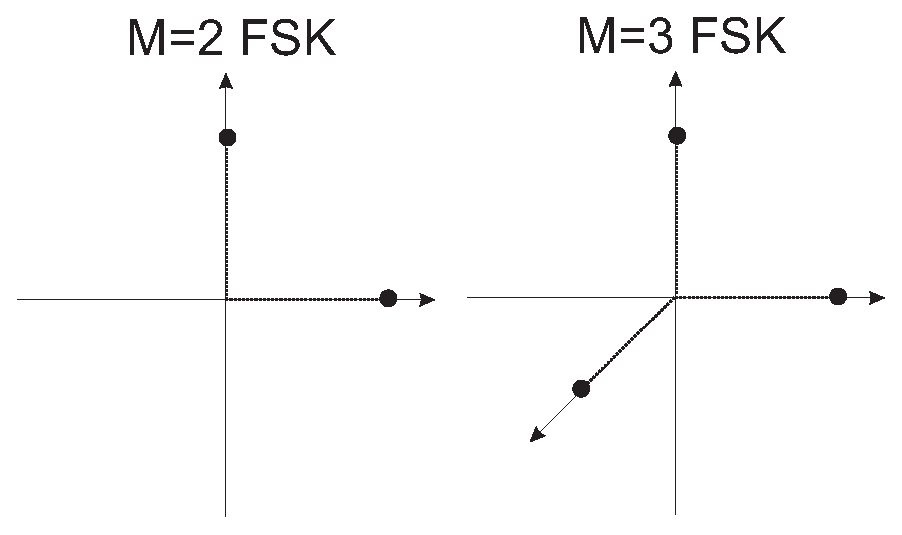
\includegraphics[width=0.4\textwidth]{../images/FSK-signalSpaceDiagram.eps}}
  \caption{Signal space diagram for $M=2$ and $M=3$ FSK modulation.}
  \label{F:FSK-signalSpaceDiagram}
\end{figure}


\subsection{Transmission of FSK}

FSK can be seen as a sum of $M$ different carrier signals, each multiplied by a pulse shape $p(t)$.  In practice, FSK signals are usually generated from a single VCO, as seen in Figure
\ref{F:FSK-TX-BlockDiagram}.

\Definition{Voltage Controlled Oscillator (VCO)}{A sinusoidal
generator with frequency that linearly proportional to an input
voltage.}

Note that we don't need to (and don't want to) send square wave input into the VCO.  The transition can be set to smoothly switch from one frequency to the next.

\Definition{Continuous Phase Frequency Shift Keying (CPFSK)}{FSK with no
phase discontinuity between symbols.  In other words, the phase of
the output signal $\phi_k(t)$ does not change instantaneously at
symbol boundaries $iT_{s}$ for integer $i$, and thus $\phi(t^- +
iT_{s}) = \phi(t^+ + iT_{s})$ where $t^-$ and $t^+$ are the
limiting times just to the left and to the right of 0,
respectively.}

There are a variety of flavors of CPFSK, which are beyond the scope of this course.

\begin{figure}[htbp]
  \centerline{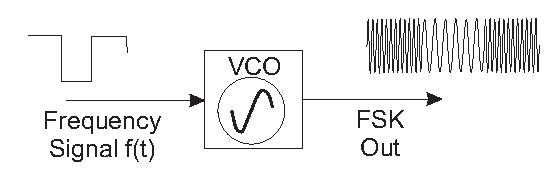
\includegraphics[width=0.6\textwidth]{../images/FSK-BlockDiagram.eps}}
  \caption{Block diagram of a binary FSK transmitter.}
  \label{F:FSK-TX-BlockDiagram}
\end{figure}

\subsection{Reception of FSK}

FSK reception is either phase coherent or phase non-coherent.  Here,
there are $M$ possible carrier frequencies, so we'd need to know and
be synchronized to $M$ different phases $\theta_i$, one for each
symbol frequency:
\begin{eqnarray}
  && \cos(\omega_0 t  + \theta_0)
    \nonumber \\
  && \cos(\omega_0 t  + 2\pi \Delta f t + \theta_1)
    \nonumber \\
    &  & \vdots \nonumber \\
  && \cos(\omega_0 t + 2\pi (M-1)\Delta f t + \theta_{M-1})
    \nonumber
\end{eqnarray}

\subsection{Coherent Reception}

FSK reception can be done via a correlation receiver, just as we've
seen for previous modulation types.

Each phase $\theta_k$ is estimated to be $\hat{\theta}_k$ by a
separate phase-locked loop (PLL). In one flavor of CPFSK (called Sunde's FSK), the carrier $\cos(2\pi f_k t + \theta_k)$ is sent with
the transmitted signal, to aid in demodulation (at the expense of
the additional energy).  This is the only case where I've heard of
using coherent FSK reception.

As $M$ gets high, coherent detection becomes difficult.  These $M$
PLLs must operate even though they can only synchronize when their
symbol is sent, $1/M$ of the time (assuming equally-probable
symbols). Also, having $M$ PLLs is a drawback.


\subsection{Non-coherent Reception}

Notice that in Figure \ref{F:FSK-signalSpaceDiagram}, the sign or
phase of the sinusoid is not very important -- only one symbol
exists in each dimension.  In non-coherent reception, we just
measure the energy in each frequency.

This is more difficult than it sounds, though -- we have a
fundamental problem. As we know, for every frequency, there are two
orthogonal functions, cosine and sine (see QAM and PSK).  Since we
will not know the phase of the received signal, we don't know
whether or not the energy at frequency $f_{k}$ correlates highly with
the cosine wave or with the sine wave.  If we only correlate it with
one (the sine wave, for example), and the phase makes the signal the
other (a cosine wave) we would get a inner product of zero!

The solution is that we need to correlate the received signal with
both a sine and a cosine wave at the frequency $f_{k}$.  This will
give us two inner products, lets call them $x_{k}^I$ using the
capital $I$ to denote in-phase and $x_{k}^Q$ with $Q$ denoting
quadrature.

\begin{figure}[htbp]
  \centerline{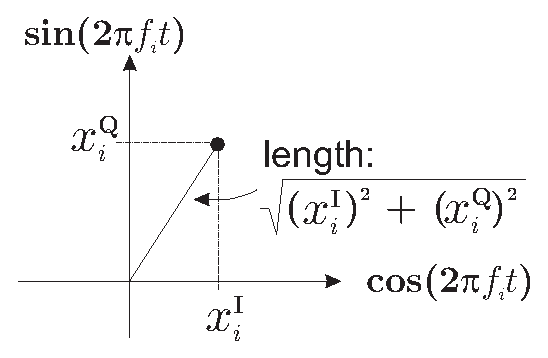
\includegraphics[width=0.45\textwidth]{../images/FSK_Energy_Diagram.eps}}
  \caption{The energy in a non-coherent FSK receiver at one frequency $f_k$ is calculated by
  finding its correlation with the cosine wave ($x_{k}^I$) and sine wave ($x_{k}^Q$) at the frequency of interest, $f_{k}$, and
  calculating the squared length of the vector $[x_{k}^I, x_{k}^Q]^T$.}
  \label{F:FSK_Energy_Diagram}
\end{figure}

The energy at frequency $f_{k}$, that is,
\[
 \En_{f_{k}} =  (x_{k}^I)^2 +  (x_{k}^Q)^2
\]
is calculated for each frequency $f_{k}$, $k=0, 1, \ldots, M-1$, and the detector picks the $k$ that maximizes $\En_{f_{k}}$.  

However, energy detection works only when $n=2$ in (\ref{E:Delta_f_FSK}).  (Showing this might be a good homework or exam problem.)  That is, $\Delta f = 1/T_s$.  Some FSK systems trade off the extra bandwidth usage in order to allow for a less complicated receiver design (an energy detector).

\subsection{Bandwidth of FSK}

Carson's rule is used to calculate the bandwidth of FM signals.  For
$M$-ary FSK, it tells us that the approximate bandwidth is,
\[
B_{M-FSK} = (M-1) \Delta f + B_{p(t)}
\]
where $B_{p(t)}$ is the two-sided bandwidth of the pulse shape.
For root raised-cosine pulse shaping, the null-to-null bandwidth is 
$B_{p(t)}=(1+\alpha)/T_s$. 


 


\StartOf{Lecture 8}

\Today{(1) OFDM and Multicarrier Modulation, (2) Probability in Digital Comms}

\announcements{
\begin{itemize}
  \item For today: Rice 5.5 and 4.1--4.3.  
  \item For Mon: Kay book reading (Canvas). Note that we meet as normal on Feb 17.
  \item HW 3 due today; Proj 2 due Mon. 
  \item HW 4 posted, due Feb 19.  
\end{itemize}
}

\section{Orthogonal Frequency Division Multiplexing (OFDM)}

This is section 5.5 in the Rice book.

In FSK, we use a single basis function at each of different
frequencies.  In QAM, we use two basis functions at the same
frequency.  \emph{Multicarrier modulation} is the combination:
\begin{eqnarray}
 \phi_{0,c}(t) &=& \sqrt{\frac{2}{T_{s}}} p(t) \cos(\omega_0 t)
 \nnn
 \phi_{0,s}(t) &=& -\sqrt{\frac{2}{T_{s}}} p(t) \sin(\omega_0 t)
 \nnn
 \phi_{1,c}(t) &=& \sqrt{\frac{2}{T_{s}}} p(t) \cos(\omega_0 t + 2\pi \Delta f t)
 \nnn
 \phi_{1,s}(t) &=& -\sqrt{\frac{2}{T_{s}}} p(t) \sin(\omega_0 t + 2\pi \Delta f t)
 \nnn
  &\vdots & \nonumber \\
 \phi_{M-1,c}(t) &=& \sqrt{\frac{2}{T_{s}}} p(t) \cos(\omega_0 t + 2\pi (M-1)\Delta f t)
 \nnn
 \phi_{M-1,s}(t) &=& -\sqrt{\frac{2}{T_{s}}} p(t) \sin(\omega_0 t + 2\pi (M-1)\Delta f t)
 \nn
\end{eqnarray}
where $\Delta f = \frac{1}{2T_{s}}$.  In OFDM, we call the two waveforms (sine and cosine) at one frequency a ``subcarrier''.  Multi-carrier modulation is a general type of modulation, of which \emph{orthogonal frequency division multiplexing} (OFDM) is a specific version which uses the NRZ (rectanguar) pulse, non-zero only between 0 and $T_s$.  OFDM is thus represented as:
\begin{eqnarray}
 \phi_{0,c}(t) &=& \pdfarray{\sqrt{\frac{2}{T_{s}}} \cos(\omega_0 t)}{0 \le t \le T_{s}}
 \nnn
 \phi_{0,s}(t) &=& \pdfarray{-\sqrt{\frac{2}{T_{s}}} \sin(\omega_0 t)}{0 \le t \le T_{s}}
 \nnn
 \phi_{1,c}(t) &=& \pdfarray{\sqrt{\frac{2}{T_{s}}} \cos(\omega_0 t + 2\pi \Delta f t)}{0 \le t \le T_{s}}
 \nnn
 \phi_{1,s}(t) &=& \pdfarray{-\sqrt{\frac{2}{T_{s}}} \sin(\omega_0 t + 2\pi \Delta f t)}{0 \le t \le T_{s}}
 \nnn
  &\vdots & \nonumber \\
 \phi_{M-1,c}(t) &=& \pdfarray{\sqrt{\frac{2}{T_{s}}} \cos(\omega_0 t + 2\pi (M-1)\Delta f t)}{0 \le t \le T_{s}}
 \nnn
 \phi_{M-1,s}(t) &=& \pdfarray{-\sqrt{\frac{2}{T_{s}}} \sin(\omega_0 t + 2\pi (M-1)\Delta f t)}{0 \le t \le T_{s}}
 \nn
\end{eqnarray}
where again $\Delta f = \frac{1}{2T_{s}}$. 

These waveforms, for multicarrier modulation and for OFDM in particular, are all mutually orthogonal, as you will show in your homework 4.  We can transmit much more information than possible in
$M$-ary FSK.  (Note we have $2M$ basis functions here in the same bandwidth as M-ary FSK!)


The signal on subchannel $k$ for OFDM might be represented as:
\[
  x_k(t) = \sqrt{\frac{2}{T_{s}}} \left[ a_{k,I}(t) \cos(\omega_0 t  + 2\pi f_k t) - a_{k,Q}(t) \sin(\omega_0 t + 2\pi f_k t) \right]
\]
On the $k$th channel, the signal could be described as some kind of QAM or PSK modulation. Regardless, over all channels, the modulation is called OFDM.  The OFDM  signal of the sum of all $K$ signals might then be represented as
\begin{eqnarray}
  x(t) &=& \sqrt{\frac{2}{T_{s}}} \mR \left\{ \sum_{k=1}^K (a_{k,I}(t) + j a_{k,Q}(t))  e^{j(\omega_0 + 2\pi k \Delta f )t}  \right\} \nonumber \\
  x(t) &=& \sqrt{\frac{2}{T_{s}}} \mR \left\{ e^{j\omega_0 t} \sum_{k=1}^K A_{k}(t)  e^{j2\pi k \Delta f t}  \right\}
\end{eqnarray}
where $A_{k}(t) = a_{k,I}(t) + j a_{k,Q}(t)$. Does this look like an
inverse discrete Fourier transform? If yes, than you can see why it
might be possible to use an IFFT and FFT to generate the transmitted signal.

\begin{enumerate}
  \item FFT implementation:  There is a particular implementation of
  the transmitter and receiver that use FFT/IFFT operations.  This
  avoids having $K$ independent transmitter chains and receiver
  chains.  The FFT implementation (and the speed and ease of implementation of the FFT in hardware) is why OFDM
  is popular.
\end{enumerate}


Since the $K$ carriers are orthogonal, the signal is like $K$-ary
FSK. But, rather than transmitting on one of the $K$ carriers at a
given time (like FSK) we transmit information in parallel on all $K$
channels simultaneously.  An example state space diagram for $K=3$
and PAM on each channel is shown in Figure
\ref{F:OFDM-state-space-diagram}.

\begin{figure}[htbp]
  \centerline{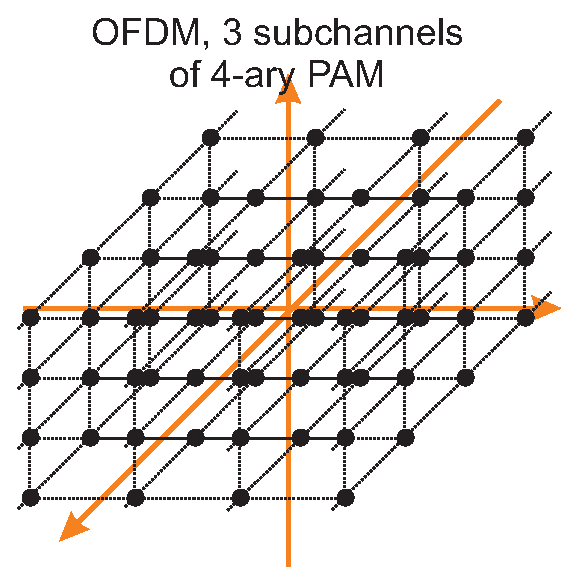
\includegraphics[width=0.45\textwidth]{../images/OFDM-K3-4PAM-signalSpaceDiagram.eps} }
  \caption{Signal space diagram for $K=3$ subchannel OFDM with 4-PAM on each channel.}
  \label{F:OFDM-state-space-diagram}
\end{figure}

\Example{802.11a}  IEEE 802.11a uses OFDM with 52 subcarriers.  Four of the subcarriers are reserved for pilot tones, so effectively 48 subcarriers are used for data.  Each data subcarrier can be modulated in different ways.  One example is to use 16 square QAM on each subcarrier (which is 4 bits per symbol per subcarrier).  The symbol rate in 802.11a is 250k/sec.  Thus the bit rate is
\[
   250\times 10^3 \frac{\mbox{OFDM symbols}}{\mbox{sec}} 48 \frac{\mbox{subcarriers}}{\mbox{OFDM symbol}} 4 \frac{\mbox{coded bits}}{\mbox{subcarrier}} = 48 \frac{\mbox{Mbits}}{\mbox{sec}}
\]



\section{Probability in Digital Communications}

Question: What is random about digital communications signals?  Why do we need probabilistic analysis tools in the design of digital communications systems?

\Solution{
Here are some of my ideas, but of course there are others:
\begin{enumerate}
    \item The data being sent
    \item Additive noise
    \item Interference from competing systems
    \item Multipath fading
    \item Doppler
    \item Transmit signal imperfections
    \item The timing of when a packet starts
    \item Transmit power
    \item Whether a receiver is awake or in sleep state at any time
    \item Frequency offset
\end{enumerate}

}

In general, random variables are (typically) unknown.  The use of probability theory and analysis is to allow us to quantify what can be known about those random systems, and to use that in engineering design of those systems.


\subsection{Distributions}

Probability distributions give us a tool to quantify how likely particular a range of values is, or even a particular value is, of a random variable.  

\vspace{0.15in}\noindent For two random variables $X_1$ and $X_2$,
\begin{itemize}
  \item Joint CDF: $F_{X_1, X_2}(x_1, x_2) = \PR{\{X_1 \le x_1\}
    \cap \{X_2 \le x_2\}}$  It is the probability that both events
    happen simultaneously.
  \item Joint pmf: $p_{X_1, X_2}(x_1, x_2) = \PR{\{X_1 = x_1\}
    \cap \{X_2 = x_2\}}$  It is the probability that both events
    happen simultaneously.
  \item Joint pdf: $f_{X_1, X_2}(x_1, x_2) = \dtwodd{x_1}{x_2} F_{X_1, X_2}(x_1, x_2)$
\end{itemize}
The (pdf / pmf) (integrates / sums) to one, and is non-negative.  The CDF is non-negative and non-decreasing, with 
$\lim_{x_i\rightarrow.-\infty} F_{X_1, X_2}(x_1, x_2) = 0$ and $\lim_{x_1,x_2 \rightarrow.+\infty} F_{X_1, X_2}(x_1, x_2) = 1$.



\vspace{0.15in}\noindent To find the probability of an event, you
integrate.  For example, for event $B \in S$,
\begin{itemize}
  \item Discrete case: $\PR{B} = \sum \sum_{(X_1,X_2) \in B} p_{X_1, X_2}(x_1, x_2)$
  \item Continuous Case: $\PR{B} = \int \int_{(x_1,x_2) \in B} f_{X_1, X_2}(x_1,  x_2) dx_1 dx_2$
\end{itemize}

\vspace{0.15in}\noindent The marginal distributions are:
\begin{itemize}
  \item Marginal pmf: $p_{X_2}(x_2) = \sum_{x_1 \in S_{X_1}} p_{X_1, X_2}(x_1, x_2)$
  \item Marginal pdf: $f_{X_2}(x_2) = \int_{x_1 \in S_{X_1}} f_{X_1, X_2}(x_1,
  x_2) dx_1$
\end{itemize}

\vspace{0.15in}\noindent Two random variables $X_1$ and $X_2$ are
independent iff for all $x_1$ and $x_2$,
\begin{itemize}
  \item $p_{X_1, X_2}(x_1, x_2) = p_{X_1}(x_1) p_{X_2}(x_2)$
  \item $f_{X_1, X_2}(x_1, x_2) = f_{X_2}(x_2) f_{X_1}(x_1)$
\end{itemize}

\subsection{Random Vectors}

\Definition{Random Vector}{A random vector (R.V.) is a list of
multiple random variables $X_1, X_2, \ldots, X_n$,
\[
\mbX = [X_1, X_2, \ldots, X_n]^T
\]
}

Here are the Models of R.V.s:
\begin{enumerate}
  \item The CDF of R.V. $\mbX$ is $F_{\mbX}(\mbx) = F_{X_1, \ldots,
    X_n}(x_1, \ldots, x_n)$ $= \PR{X_1 \le x_1, \ldots, X_n \le x_n}$.
  \item The pmf of a discrete R.V. $\mbX$ is $p_{\mbX}(\mbx) $ $= p_{X_1, \ldots,
    X_n}(x_1, \ldots, x_n) $  $= \PR{X_1 = x_1, \ldots, X_n = x_n}$.
  \item The pdf of a continuous R.V. $\mbX$ is $f_{\mbX}(\mbx) $ $= f_{X_1, \ldots,
    X_n}(x_1, \ldots, x_n) $ $= \tfrac{\partial^n}{\partial x_1 \cdots \partial x_n} F_{\mbX}(\mbx)$.
\end{enumerate}

\subsection{Conditional Distributions}

\vspace{0.15in}\noindent Given event $B \in S$ which has $\PR{B}>0$,
the joint probability conditioned on event $B$ is
\begin{itemize}
  \item Discrete case:
    \[ p_{X_1, X_2 | B}(x_1, x_2) = \pdfarray{\frac{p_{X_1, X_2}(x_1, x_2)}{ \PR{B}}}{(X_1, X_2) \in B}
    \]
  \item Continuous Case:
    \[ f_{X_1, X_2 | B}(x_1, x_2) = \pdfarray{\frac{f_{X_1, X_2}(x_1, x_2)}{ \PR{B}}}{(X_1, X_2) \in B}
    \]
\end{itemize}

\vspace{0.15in}\noindent Given r.v.s $X_1$ and $X_2$,
\begin{itemize}
  \item Discrete case.  The conditional pmf of $X_1$ given $X_2=x_2$, where $p_{X_2}(x_2) > 0$, is
    \[ p_{X_1| X_2 }(x_1| x_2) = p_{X_1, X_2}(x_1 , x_2) / p_{X_2}(x_2)
    \]
  \item Continuous Case:  The conditional pdf of $X_1$ given
  $X_2=x_2$, where $f_{X_2}(x_2) > 0$, is
    \[ f_{X_1| X_2 }(x_1| x_2) = f_{X_1, X_2}(x_1, x_2) / f_{X_2}(x_2)
    \]
\end{itemize}

\Definition{Bayes' Law}{Bayes' Law is a reformulation of he
definition of the marginal pdf.  It is written either as:
  \[
      f_{X_1,X_2}(x_1,x_2) = f_{X_2|X_1}(x_2|x_1) f_{X_1}(x_1)
  \]
  or
  \[
      f_{X_1|X_2}(x_1|x_2) = \frac{f_{X_2|X_1}(x_2|x_1)
      f_{X_1}(x_1)}{f_{X_2}(x_2)}
  \]
}

\subsection{Simulation of Digital Communication Systems}

A simulation of a digital communication system is often used to
estimate a bit error rate.  Each bit can either be demodulated
without error, or with error.  Thus the simulation of one bit is a
Bernoulli trial.  This trial $E_i$ is in error ($E_1=1$) with
probability $p_e$ (the true bit error rate) and correct ($E_i=0$)
with probability $1-p_e$.  What type of random variable is $E_i$?

Simulations run many bits, say $N$ bits through a model of the
communication system, and count the number of bits that are in
error.  Let $S = \sum_{i=1}^N E_i$, and assume that $\{E_i\}$ are
independent and identically distributed (i.i.d.).
\begin{enumerate}
  \item What type of random variable is $S$?
  \item What is the pmf of $S$?
  \item What is the mean and variance of $S$?
\end{enumerate}

\Solution{$E_i$ is called a Bernoulli r.v.~and $S$ is called a Binomial r.v., with pmf
\[
  p_S(s) = {N \choose s} p_e^s (1-p_e)^{N-s}
\]
The mean of $S$ is the the same as the mean of the sum of $\{E_i\}$,
\begin{eqnarray}
  \E{S}{S} &=& \E{\{E_i\}}{\sum_{i=1}^N E_i} = \sum_{i=1}^N  \E{E_i}{E_i} \nnn
   &=& \sum_{i=1}^N   \left[ (1-p)\cdot 0 + p \cdot 1\right] = Np \nn
\end{eqnarray}
We can find the variance of $S$ the same way:
\begin{eqnarray}
  \Var{S}{S} &=& \Var{\{E_i\}}{\sum_{i=1}^N E_i} = \sum_{i=1}^N  \Var{E_i}{E_i} \nnn
   &=& \sum_{i=1}^N   \left[ (1-p)\cdot (0-p)^2 + p \cdot (1-p)^2\right]
   \nnn
   &=& \sum_{i=1}^N   \left[ (1-p)p^2 + (1-p)(p-p^2)\right] 
   \nnn
   &=&   Np(1-p)
   \nn
\end{eqnarray}
}

We may also be interested knowing how many bits to run in order to
get an estimate of the bit error rate.  For example, if we run a
simulation and get zero bit errors, we won't have a very good idea
of the bit error rate.  Let $T_1$ be the time (number of bits) up to and including the first error.
\begin{enumerate}
  \item What type of random variable is $T_1$?
  \item What is the pmf of $T_1$?
  \item What is the mean of $T_1$?
\end{enumerate}

\Solution{$T_1$ is a Geometric r.v. with pmf
\[
  p_{T_1}(t) = (1-p_e)^{t-1} p_e
\]
The mean of $T_1$ is
\[
  \E{}{T_1} = \frac{1}{p_e}
\]
Note the variance of $T_1$ is $\Var{}{T_1} = (1-p_e)/p_e^2$, so the
standard deviation for very low $p_e$ is almost the same as the
expected value.}

So, even if we run an experiment until the first bit error, our
estimate of $p_e$ will have relatively high variance.

% \subsection{Mixed Discrete and Continuous Joint Variables}
% 
% This was not covered in ECE 5510, although it was in the Yates \&
% Goodman textbook.  We'll often have $X_1$ discrete and $X_2$
% continuous.
% 
% \Example{Digital communication system in noise} Let $X_1$ is the
% transmitted signal voltage, and $X_2$ is the received signal
% voltage, which is modeled as
% \[
% X_2 = a X_1 + N
% \]
% where $N$ is a continuous-valued random variable representing the
% additive noise of the channel, and $a$ is a constant which
% represents the attenuation of the channel.  In a digital system,
% $X_1$ may take a discrete set of values, \eg, $\{ 1.5, 0.5, -0.5,
% -1.5\}$.  But the noise $N$ may be continuous, \eg, Gaussian with
% mean $\mu$ and variance $\sigma^2$.  As long as $\sigma^2>0$, then
% $X_2$ will be continuous-valued.
% 
% \vspace{0.15in}\noindent \textbf{Work-around}:  We will sometimes
% use a pdf for a discrete random variable.  For instance, if
% \[
%   p_{X_1}(x_1) = \pdfarrays{0.6}{x_1 = 0}{0.4}{x_1=1}
% \]
% then we would write a pdf with the probabilities as amplitudes of a
% dirac delta function centered at the value that has that
% probability,
% \[
%   f_{X_1}(x_1) = 0.6\delta(x_1) + 0.4\delta(x_1-1)
% \]
% This pdf has integral 1, and non-negative values for all $x_1$.  Any
% probability integral will return the proper value.  For example, the
% probability that $-0.5 < x_1 < 0.5$ would be an integral that would
% return 0.6.
% 
% \Example{Joint distribution of $X_1, X_2$} Consider the channel
% model $X_2 = X_1 + N$, and
% \[
%  f_N(n) = \frac{1}{\sqrt{2\pi \sigma^2}} e^{-n^2/(2\sigma^2)}
% \]
% where $\sigma^2$ is some known variance, and the r.v. $X_1$ is
% independent of $N$ with
% \[
%   p_{X_1}(x_1) = \pdfarrays{0.5}{x_1 = 0}{0.5}{x_1=1}.
% \]
% \begin{enumerate}
%   \item What is the pdf of $X_2$?
%   \item What is the joint p.d.f.~of $(X_1, X_2)$ ?
% \end{enumerate}
% 
% \Solution{
% \begin{enumerate}
%   \item When two independent r.v.s are added, the pdf of the sum is the
%     \emph{convolution} of the pdfs of the inputs.  Writing
%     \[
%       f_{X_1}(x_1) = 0.5 \delta(x_1) + 0.5 \delta(x_1-1)
%     \]
%     we convolve this with $f_N(n)$ above, to get
%     \begin{eqnarray}
%       f_{X_2}(x_2) &=& 0.5 f_N(x_2) + 0.5f_N(x_2-1) \nonumber \\
%       f_{X_2}(x_2) &=& \frac{1}{2\sqrt{2\pi \sigma^2}} \left[
%           e^{-x_2^2/(2\sigma^2)} + e^{-(x_2-1)^2/(2\sigma^2)}
%         \right] \nonumber
%     \end{eqnarray}
%   \item What is the joint p.d.f.~of $(X_1, X_2)$ ?
%     Since $X_1$ and $X_2$ are NOT independent, we cannot simply multiply
%     the marginal pdfs together.  It is necessary to use Bayes' Law.
%     \[
%       f_{X_1,X_2}(x_1,x_2) = f_{X_2|X_1}(x_2|x_1) f_{X_1}(x_1)
%     \]
%     Given a value of $X_1$ (either 0 or 1) we can write down the pdf
%     of $X_2$.  So break this into two cases:
%     \begin{eqnarray}
%        f_{X_1,X_2}(x_1,x_2) &=& \pdfarrays{f_{X_2|X_1}(x_2|0)
%          f_{X_1}(0)}{x_1 = 0}{f_{X_2|X_1}(x_2|1)
%          f_{X_1}(1)}{x_1 = 1} \nonumber \\
%        f_{X_1,X_2}(x_1,x_2) &=& \pdfarrays{ 0.5 f_N(x_2)}{x_1 = 0}{0.5f_N(x_2-1)}{x_1 = 1} \nonumber \\
%        f_{X_1,X_2}(x_1,x_2) &=& 0.5 f_N(x_2) \delta(x_1)  + \nnn
%                             & & 0.5 f_N(x_2-1) \delta(x_1 - 1) \nonumber
%     \end{eqnarray}
%     These last two lines are completely equivalent.  Use
%     whichever seems more convenient for you.  See Figure
%     \ref{F:MixedPdfExample}.
% \end{enumerate}
% }
% \begin{figure}[htb]
%   \centerline{\psfig{figure=plotMixedPdfExample.eps,width=3in}}
%   \caption{Joint pdf of $X_1$ and $X_2$, the input and output (respectively) of the example additive noise communication system, when $\sigma=1$.}
%   \label{F:MixedPdfExample}
% \end{figure}

\subsection{Expectation}

\Definition{Expected Value (Joint)}{ The expected value of a
function $g(X_1, X_2)$ of random variables $X_1$ and $X_2$ is given
by,
\begin{enumerate}
  \item Discrete: $\E{}{g(X_1, X_2)} =
     \sum_{X_1 \in S_{X_1}} \sum_{X_2 \in S_{X_2}} g(X_1, X_2) p_{X_1, X_2}(x_1, x_2)$
  \item Continuous: $\E{}{g(X_1, X_2)} =
     \int_{X_1 \in S_{X_1}} \int_{X_2 \in S_{X_2}} g(X_1, X_2) f_{X_1, X_2}(x_1, x_2)$
\end{enumerate}}

Typical functions $g(X_1, X_2)$  are:
\begin{itemize}
  \item Mean of $X_1$ or $X_2$:  $g(X_1, X_2) = X_1$ or $g(X_1, X_2) =
    X_2$ will result in the means $\mu_{X_1}$ and $\mu_{X_2}$.
  \item Variance (or 2nd central moment) of $X_1$ or $X_2$:  $g(X_1, X_2) = (X_1-\mu_{X_1})^2$ or $g(X_1, X_2) =
    (X_2-\mu_{X_2})^2$.  Often denoted $\sigma_{X_1}^2$ and
    $\sigma_{X_2}^2$.
  \item Covariance of $X_1$ and $X_2$: $g(X_1, X_2) =
    (X_1-\mu_{X_1})(X_2-\mu_{X_2})$.
  \item Expected value of the product of $X_1$ and $X_2$, also called the `correlation' of $X_1$ and $X_2$: $g(X_1, X_2) =
    X_1 X_2$.
\end{itemize}

% Stopped here, S09 Lecture 6.

\subsection{Gaussian Random Variables}

For a single Gaussian r.v. $X$ with mean $\mu_X$ and variance
$\sigma_X^2$, we have the pdf,
\[
  f_X(x) = \frac{1}{\sqrt{2\pi \sigma_X^2}} e^{-\frac{(x-\mu_X)^2}{2\sigma^2}}
\]
Consider $Y$ to be Gaussian  with mean 0 and variance 1.  The distribution of $Y$ is also called \emph{standard normal} in the statistics community without any sense of shame for the redundancy of the two words.  Regardless, we define a new symbol for the CDF of standard normal r.v.\ $Y$: 
CDF of $Y$ is denoted as $F_Y(y) = \PR{Y \le y} = \Phi(y)$.  So, for
$X$, which has non-zero mean and non-unit-variance, we can write its
CDF as
\[
  F_X(x) = \PR{X\le x} = \Phi \left( \frac{x-\mu_X}{\sigma_X} \right)
\]
You can prove this by showing that the event $X \le x$ is the same
as the event
\[
  \frac{X-\mu_X}{\sigma_X} \le \frac{x-\mu_X}{\sigma_X}
\]
Since the left-hand side is a unit-variance, zero mean Gaussian
random variable, we can write the probability of this event using
the unit-variance, zero mean Gaussian CDF.

\subsubsection{Complementary CDF}
The probability that a unit-variance, zero mean Gaussian r.v. $X$ exceeds some value $x$ is one minus the
CDF, that is, $1-\Phi(x)$.  This is so common in digital communications, it is given its
own name, $Q(x)$,
\[
  Q(x) = \PR{X >  x} = 1 - \Phi \left( x \right)
\]
What is $Q(x)$ in integral form?
\[
  Q(x) = \int_x^\infty \frac{1}{\sqrt{2\pi}} e^{-w^2/2} dw
\]
For an Gaussian r.v. $X$ with variance $\sigma_X^2$,
\[
  \PR{X >  x} = Q\left( \frac{x-\mu_X}{\sigma_X} \right)  = 1 - \Phi \left( \frac{x-\mu_X}{\sigma_X} \right)
\]

\subsubsection{Error Function}

In math, in some texts, and in Matlab, the $Q(x)$ function is not
used.  Instead, there is a function called $\erf(x)$
\[
  \erf(x) \triangleq \frac{2}{\sqrt{\pi}} \int_0^x e^{-t^2} dt
\]


\Example{Relationship between $Q(\cdot)$ and $\erf(\cdot)$}  What is
the functional relationship between $Q(\cdot)$ and $\erf(\cdot)$?

\Solution{ Substituting $t=u/\sqrt{2}$ (and thus $dt =
  du/\sqrt{2}$),
  \begin{eqnarray}
    \erf(x) &\triangleq& \frac{2}{\sqrt{2\pi}} \int_0^{\sqrt{2}x} e^{-u^2/2}
    du \nonumber \\
            &=& 2 \int_0^{\sqrt{2}x} \frac{1}{\sqrt{2\pi}} e^{-u^2/2}
    du \nonumber \\
            &=& 2  \left( \Phi(\sqrt{2}x) - \frac{1}{2} \right) \nonumber
  \end{eqnarray}
  Equivalently, we can write $\Phi(\cdot)$ in terms of the
  $\erf(\cdot)$ function,
  \[
    \Phi(\sqrt{2}x) = \frac{1}{2} \erf(x) + \frac{1}{2}
  \]
  Finally  let $y=\sqrt{2}x$, so that
  \[
    \Phi(y) = \frac{1}{2} \erf\left(\frac{y}{\sqrt{2}}\right) + \frac{1}{2}
  \]
  Or in terms of $Q(\cdot)$,
  \begin{equation}\label{E:QInTermsOfErf}
    Q(y) = 1-\Phi(y) = \frac{1}{2} - \frac{1}{2} \erf\left(\frac{y}{\sqrt{2}}\right)
  \end{equation}
}
You should go to Matlab and create a function Q(y) which implements:
\begin{verbatim}
    function rval = Q(y)
    rval = 0.5.*erfc(y./sqrt(2));
\end{verbatim}
In Python there is an erfc function in both math and scipy.special packages.

 \Example{Probability of Error in Binary Example} As in the
previous example, we have a model system in which the receiver sees
$X_2 = X_1 + N$.  Here, $X_1 \in \{0,1\}$ with equal probabilities
and $N$ is independent of $X_1$ and zero-mean Gaussian with variance
$1/4$. The receiver decides as follows:
\begin{itemize}
  \item If $X_2 \le 1/3$, then decide that the transmitter sent a `0'.
  \item If $X_2 > 1/3$, then decide that the transmitter sent a `1'.
\end{itemize}
\begin{enumerate}
  \item Given that $X_1=1$, what is the probability that the receiver decides that a `0' was sent?
  \item Given that $X_1=0$, what is the probability that the receiver decides that a `1' was sent?
\end{enumerate}

\Solution{
  \begin{enumerate}
    \item Given that $X_1=1$, since $X_2 = X_1 + N$, it is clear that $X_2$ is also a Gaussian r.v. with mean 1 and variance 1/4.
          Then the probability that the receiver decides `0' is the
          probability that $X_2 \le 1/3$,
          \begin{eqnarray}
            \PR{error | X_1=1} &=& \PR{X_2 \le 1/3}
            = \PR{\frac{X_2-1}{\sqrt{1/4}} \le \frac{1/3 - 1}{\sqrt{1/4}}}
                \nonumber \\
            &=& 1 - Q \left( (-2/3)/(1/2) \right) 
                = 1- Q(-4/3)
                \nonumber
          \end{eqnarray}
    \item Given that $X_1=0$, the probability that the receiver decides `1' is the
          probability that $X_2 > 1/3$,
          \begin{eqnarray}
            \PR{error | X_1=0} &=& \PR{X_2 > 1/3}
            = \PR{\frac{X_2}{\sqrt{1/4}} > \frac{1/3}{\sqrt{1/4}}}
                \nonumber \\
            &=& Q \left( (1/3)/(1/2) \right) 
            = Q(2/3)
                \nonumber
          \end{eqnarray}
  \end{enumerate}
}




 \StartOf{Lecture 9}

\Today{(0) Gaussan r.v.s from Lecture 8, (1) 1-D Detection }

\announcements{
\begin{itemize}
  \item Project 2 due today, 11:59pm.  HW 4 due Wednesday.
  \item Reading: today: Stephen M. Kay, ``Detection Theory'' Chapter 3.3 \& 3.6 (pdf on Canvas).  Wed: Rice 4.4-4.5
\end{itemize}
}

\section{Bayesian 1-D Detection}

When we say `optimal detection' in the Bayesian detection framework,
we mean that we want the smallest probability of error.  The
probability of error is denoted
\[
  \PR{\mbox{symbol error}}
\]
By error, we mean that a different symbol was detected than the symbol
that was sent.   At the start of every detection problem, we list the
events that could have occurred, \ie, the symbols that could have
been sent. We follow all detection and statistics textbooks and label these classes $H_i$.

Later we will use detection theory to describe why we use a matched filter.  For now, we're studying a somewhat simpler problem, assuming that our receiver uses a matched filter, time synchronization block, and downsampling block.
Our receivers need to make a decision after the downsampling. based on the voltages $X_i$ measured at this point, for each waveform $\phi_i(t)$.  Further for this lecture, we are studying the case when there is only one waveform, e.g., PAM.  Thus we call this voltage $X$ for simplicity.  The voltage $X$ should be close to one of $M$ possible symbol values $a_0, \ldots, a_{M-1}$.  

In summary we describe the decision as a list of \emph{models} that describe what the conditional distribution of $X$ is given that the $i$th symbol is sent:
\begin{eqnarray}
  H_0: && X = a_0 + W \nonumber \\
  H_1: && X = a_1 + W \nonumber \\
  \cdots && \cdots \nonumber \\
  H_{M-1}: && X = a_{M-1} + W \nonumber
\end{eqnarray}
where $W$ is Gaussian additive noise with mean 0 and variance $\sigma^2$.
This must be a complete listing of events.  That is, the events $H_0
\cup H_1 \cup \cdots \cup H_{M-1} = S$, where the $\cup$ means
union, and $S$ is the complete event space.



Let's just say for now that there are only two symbols, i.e., $M=2$.  We
need to decide from $X$ whether symbol 0 or symbol 1 was sent.

The hypotheses are:
\begin{eqnarray}
  H_0: && X = a_0 + W \nonumber \\
  H_1: && X = a_1 + W \nonumber
\end{eqnarray}  % pause.

We use the law of total probability to say that
\begin{eqnarray}
  \PR{\mbox{error}}    &=& \PR{\mbox{error} \cap H_0} +  \PR{\mbox{error} \cap H_1 }
\end{eqnarray}
Where the cap means `and'. Then using Bayes' Law,
\[
   \PR{\mbox{error}}  = \PR{\mbox{error} | H_0}\PR{H_0} +  \PR{\mbox{error} | H_1 }\PR{H_1}
\]

\subsection{Decision Region}

We're making a decision based only on $X$.  Over some set $R_0$ of
values of $X$, we'll decide that $H_0$ happened (symbol 0 was sent).
Over a different set $R_1$ of values, we'll decide $H_1$ occurred
(that symbol 1 was sent).  \emph{We can't be indecisive}, so
\begin{itemize}
  \item There is no overlap: $R_0 \cap R_1 = \emptyset$.
  \item There are no values of $x$ disregarded: $R_0 \cup R_1 = S$.
\end{itemize}

\subsection{Formula for Probability of Error}

So the probability of error is
\begin{equation} \label{E:PeBayesianBasic}
   \PR{\mbox{error}}  = \PR{X \in R_1 | H_0}\PR{H_0} +  \PR{X \in R_0 | H_1 }\PR{H_1}
\end{equation}
The probability that $X$ is in $R_1$ is one minus the probability
that it is in $R_0$, since the two are complementary sets.
\begin{eqnarray}
   \PR{\mbox{error}}  &=& (1 - \PR{X \in R_0 | H_0} )\PR{H_0} +  \PR{X \in R_0 | H_1 }\PR{H_1}
     \nonumber \\
   \PR{\mbox{error}}  &=& \PR{H_0} - \PR{X \in R_0 | H_0} \PR{H_0} +  \PR{X \in R_0 | H_1 }\PR{H_1}
     \nonumber
\end{eqnarray}
Now note that probabilities that $X \in R_0$ are integrals over the
 event (region) $R_0$.
\begin{eqnarray}
   \PR{\mbox{error}}  &=& \PR{H_0} - \int_{x \in R_0} f_{X|H_0}(x| H_0) \PR{H_0}
   dx \nnn
     &&                             +  \int_{x \in R_0} f_{X|H_1}(x | H_1) \PR{H_1} dx
     \nonumber \\
     &=& \PR{H_0} +     \label{E:PeAsAFcnOfR1} \\
     && \int_{x \in R_0} \left\{f_{X|H_1}(x | H_1) \PR{H_1} - f_{X|H_0}(x| H_0) \PR{H_0} \right\}
     dx \nn
\end{eqnarray}
We've got a lot of things in the expression in
(\ref{E:PeAsAFcnOfR1}), but the only thing we can change is the
region $R_0$.  Everything else is determined by the time we get to
this point.  So the question is, how do you pick $R_0$ to minimize
(\ref{E:PeAsAFcnOfR1})?

\subsection{Selecting $R_0$ to Minimize Probability of Error}

We can see what the integrand looks like.  Figure
\ref{F:plotLikelihoodFunctionsBinaryRx}(a) shows the conditional
probability density functions.  Figure \ref{F:plotLikelihoodFunctionsBinaryRx}(b)
shows the joint densities (the conditional pdfs multiplied by the
bit probabilities $\PR{H_0}$ and $\PR{H_1}$.  Finally, Figure
\ref{F:plotLikelihoodFunctionsBinaryRx}(c) shows the full integrand of
(\ref{E:PeAsAFcnOfR1}), the difference between the joint densities.
\begin{figure}[htbp]
  \centerline{(a) 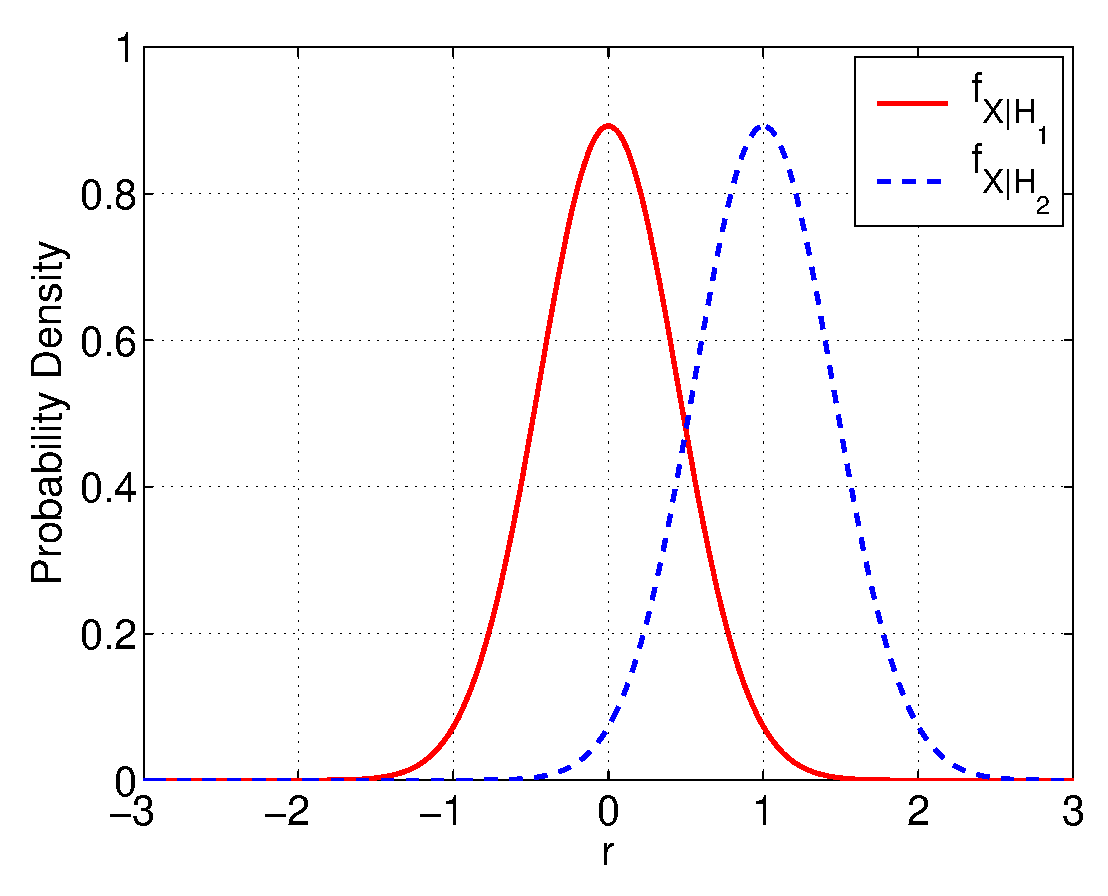
\includegraphics[width=3in]{../images/plotLikelihoodFunctionsBinaryRx.eps}}
  \centerline{(b) 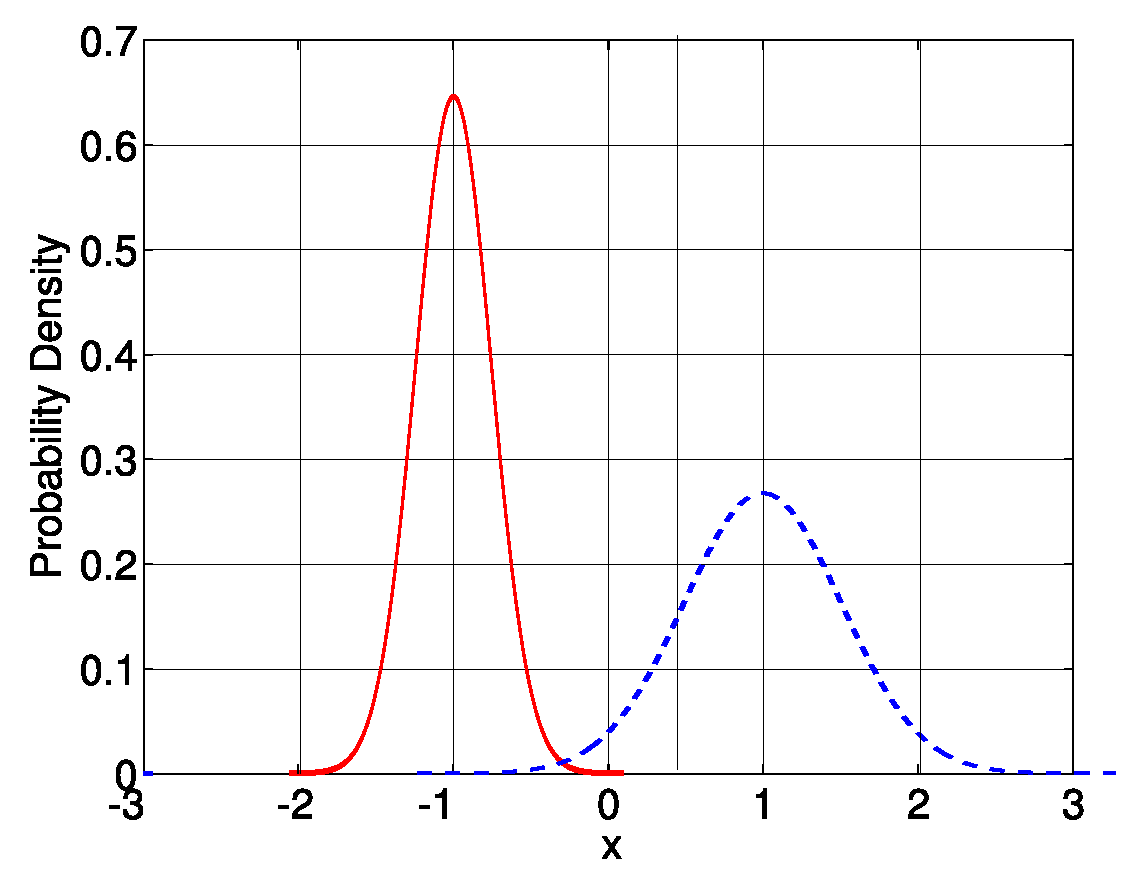
\includegraphics[width=3in]{../images/plotJointDensities.eps}}
  \centerline{(c) 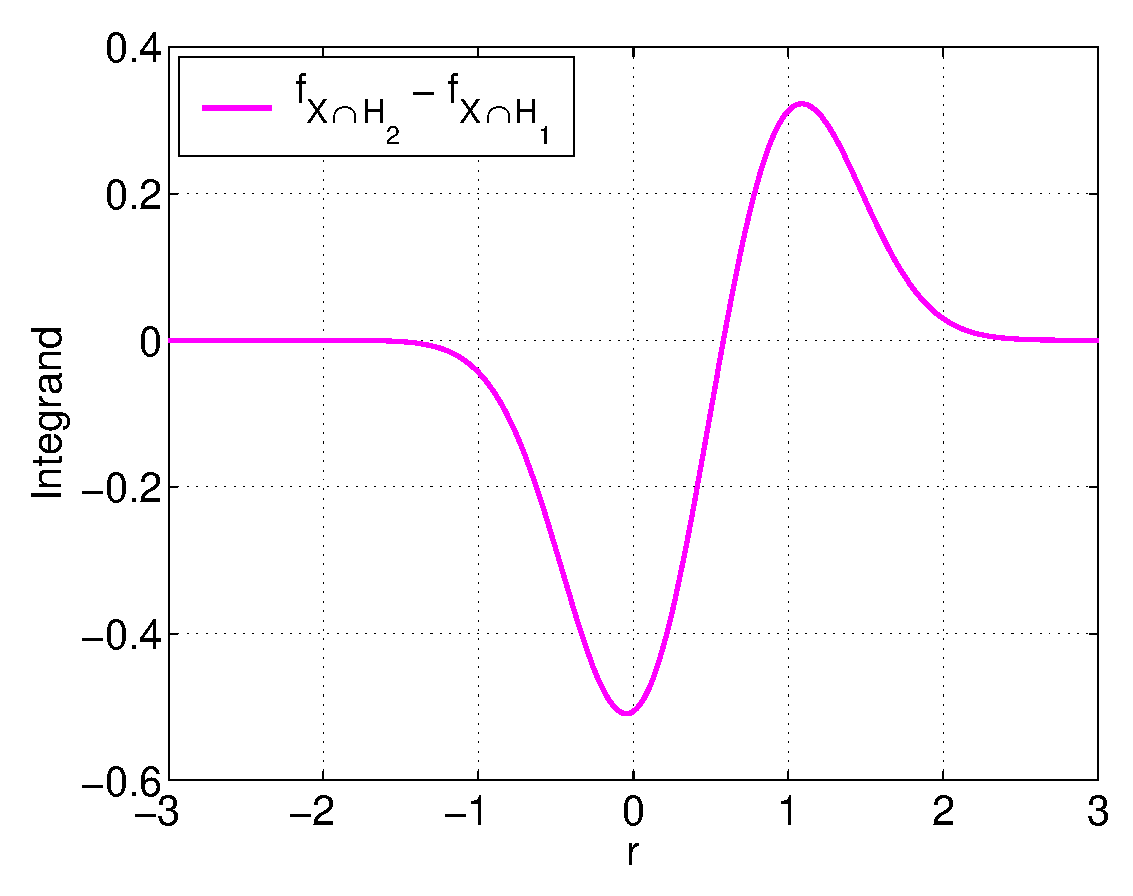
\includegraphics[width=3in]{../images/plotJointDensityDifference.eps}}
  \caption{The (a) conditional p.d.f.s (likelihood functions) $f_{X|H_0}(x|H_0)$ and $f_{X|H_1}(x|H_1)$, (b) joint p.d.f.s $f_{X|H_0}(x|H_0)\PR{H_0}$ and $f_{X|H_1}(x|H_1)\PR{H_1}$, and (c) difference between the joint p.d.f.s,
  $f_{X|H_1}(x|H_1)\PR{H_1} - f_{X|H_0}(x|H_0)\PR{H_0}$,
  which is the integrand in (\ref{E:PeAsAFcnOfR1}).}
  \label{F:plotLikelihoodFunctionsBinaryRx}
\end{figure}
% \begin{figure}[hp]
%   \caption{The joint p.d.f.s $f_{X|H_0}(x|H_0)\PR{H_0}$ and $f_{X|H_1}(x|H_1)\PR{H_1}$.}
%   \label{F:plotJointDensities}
% \end{figure}
% \begin{figure}[hp]
%   \caption{The difference between the joint p.d.f.s,
%   $f_{X|H_1}(x|H_1)\PR{H_1} - f_{X|H_0}(x|H_0)\PR{H_0}$,
%   which is the integrand in (\ref{E:PeAsAFcnOfR1}).}
%   \label{F:plotJointDensityDifference}
% \end{figure}

We can pick $R_0$ however we want - we just say what region of $x$,
and the integral in (\ref{E:PeAsAFcnOfR1}) will integrate over it.
The objective is to minimize the probability of error.  Which $x$'s
should we include in the region?  Should we include $x$ which has a
positive value of the integrand?  Or should we include the parts of
$x$ which have a negative value of the integrand?

\Solution{Select $R_0$ to be all $x$ such that the integrand is
negative.}

Then $R_0$ is the area in which
\[
  f_{X|H_0}(x|H_0) \PR{H_0} > f_{X|H_1}(x|H_1) \PR{H_1}
\]
If $\PR{H_0} = \PR{H_1}$, then this is the region in which $X$ is
more probable given $H_0$ than given $H_1$.

Rearranging the terms,
\begin{equation} \label{E:BayesianLikelihoodRatio}
  \frac{f_{X|H_1}(x|H_1)}{f_{X|H_0}(x|H_0)}  < \frac{\PR{H_0}}{ \PR{H_1}}
\end{equation}
The left hand side is called the likelihood ratio.  The right hand
side is a threshold.  Whenever $x$ indicates that the likelihood
ratio is less than the threshold, then we'll decide $H_0$, \ie, that
$s_0(t)$ was sent.  Otherwise, we'll decide $H_1$, \ie, that
$s_1(t)$ was sent.

Equation (\ref{E:BayesianLikelihoodRatio}) is a very general result,
applicable no matter what conditional distributions $x$ has.

\subsection{Log-Likelihood Ratio}

For the Gaussian distribution, the math gets much easier if we take
the log of both sides.  Why can we do this?

\Solution{ 1.  Both sides are positive, 2. The $\log()$ function is
strictly increasing.}

Now, the \emph{log-likelihood ratio} is
\[
  \log \frac{f_{X|H_1}(x|H_1)}{f_{X|H_0}(x|H_0)}  < \log \frac{\PR{H_0}}{ \PR{H_1}}
\]

\subsection{Case of $a_0 = 0$, $a_1 = 1$ in Gaussian noise}

In this example, $W \sim \mathcal{N}(0,\sigma_w^2)$.  In addition,
assume for a minute that $a_0 = 0$ and $a_1 = 1$.  What is:
\begin{enumerate}
  \item The log of a Gaussian pdf?
  \item The log-likelihood ratio?
  \item The decision regions for $x$?
\end{enumerate}

\Solution{ What is the log of a Gaussian pdf?
\begin{eqnarray}
 \log f_{X|H_0}(x|H_0) &=& \log \left[ \frac{1}{\sqrt{2\pi \sigma_w^2}} e^{-\frac{x^2}{2\sigma_w^2}} \right]
   \nonumber \\
 &=& -\frac{1}{2}\log (2\pi \sigma_w^2)  - \frac{x^2}{2\sigma_w^2}
\end{eqnarray}
The $\log f_{X|H_1}(x|H_1)$ term will be the same but with
$(x-1)^2$instead of $x^2$. Continuing with the log-likelihood ratio,
\begin{eqnarray}
   \log f_{X|H_1}(x|H_1) - \log f_{X|H_0}(x|H_0)  &<& \log \frac{\PR{H_0}}{ \PR{H_1}} \nonumber \\
   \frac{x^2}{2\sigma_w^2} - \frac{(x-1)^2}{2\sigma_w^2}  &<& \log \frac{\PR{H_0}}{ \PR{H_1}} \nonumber \\
   x^2 - (x-1)^2  &<& 2\sigma_w^2 \log \frac{\PR{H_0}}{ \PR{H_1}} \nonumber \\
   2x - 1  &<& 2\sigma_w^2 \log \frac{\PR{H_0}}{ \PR{H_1}} \nonumber \\
   x  &<& \frac{1}{2} + \sigma_w^2 \log \frac{  \PR{H_0}}{ \PR{H_1}} \nonumber
\end{eqnarray}
}

In the end result, there is a simple test for $x$ - if it is below
the \emph{decision threshold}, decide $H_0$.  If it is above the
decision threshold,
\[
x  > \frac{1}{2} + \sigma_w^2 \log \frac{  \PR{H_0}}{ \PR{H_1}}
\]
decide $H_1$.  Rather than writing both inequalities each time, we
use the following notation:
\[
 x  \decision{H_1}{H_0} \frac{1}{2} + \sigma_w^2 \log \frac{  \PR{H_0}}{\PR{H_1}}
\]
This completely describes the detector receiver.

For simplicity, we also write $x  \decision{H_1}{H_0} \gamma$ where
\begin{equation} \label{E:decisionThreshold}
  \gamma = \frac{1}{2} + \sigma_w^2 \log \frac{  \PR{H_0}}{\PR{H_1}}
\end{equation}

\subsection{General Case for Arbitrary Symbols}

If, instead of $a_0 = 0$ and $a_1 = 1$, we had arbitrary values for
them (the signal space representations of $s_0(t)$ and $s_1(t)$), we
could have derived the result in the last section the same way.  As
long as $a_0 < a_1$, we'd still have $r \decision{H_1}{H_0} \gamma$,
but now,
\begin{equation} \label{E:decisionThresholdGeneral}
  \gamma = \frac{a_0 + a_1}{2} + \frac{\sigma_w^2}{a_1 - a_0} \log \frac{  \PR{H_0}}{\PR{H_1}}
\end{equation}

\subsection{Equi-probable Special Case}

If symbols are equally likely, $\PR{H_1} = \PR{H_0}$, then
$\frac{\PR{H_1}}{  \PR{H_0}} = 1$ and the logarithm of the fraction
is zero.  So then
\[
 x  \decision{H_1}{H_0} \frac{a_0 + a_1}{2}
\]
The decision above says that if $x$ is closer to $a_0$, decide that
$s_0(t)$ was sent. And if $x$ is closer to $a_1$, decide that
$s_1(t)$ was sent. The boundary is exactly half-way in between the
two signal space vectors.

This receiver is also called a maximum likelihood detector, because
we only decide which likelihood function is higher (neither is
scaled by the prior probabilities $\PR{H_0}$ or $\PR{H_1}$.

\subsection{Examples}

\Example{When $H_1$ becomes less likely, which direction will the
optimal threshold move, towards $a_0$ or towards $a_1$?}

\Solution{Towards $a_1$.}

\Example{Let $a_0 = -1$, $a_1 = 1$, $\sigma_w^2 = 0.1$, $\PR{H_1} =
0.4$, and $\PR{H_0}=0.6$.  What is the decision threshold for $x$?}

\Solution{ From (\ref{E:decisionThresholdGeneral}),
\[
  \gamma = 0 + \frac{0.1}{2} \log \frac{0.6}{0.4} = 0.05 \log 1.5
  \approx 0.0203
\]
}

\Example{Can the decision threshold be higher than both $a_0$ and
$a_1$ in this binary, one-dimensional modulation, receiver?}

\Solution{Yes, it can.  You can make $\log \frac{  \PR{H_0}}{\PR{H_1}}$ arbitrarily high, try it!}

Given $a_0$, $a_1$, $\sigma_w^2$, $\PR{H_1}$, and $\PR{H_0}$, you
should be able to calculate the optimal decision threshold $\gamma$.

\Example{In this example, given all of the above constants and the optimal threshold $\gamma$,
calculate the probability of error from (\ref{E:PeBayesianBasic}).}
Starting from
\[
   \PR{\mbox{error}}  = \PR{x \in R_1 | H_0}\PR{H_0} +  \PR{x \in R_0 | H_1 }\PR{H_1}
\]
we can use the decision regions in (\ref{E:decisionThreshold}) to
write
\[
   \PR{\mbox{error}}  = \PR{x > \gamma | H_0}\PR{H_0} +  \PR{x < \gamma | H_1 }\PR{H_1}
\]
What is the first probability, given that $r|H_0$ is Gaussian with
mean $a_0$ and variance $\sigma_w^2$?  What is the second
probability, given that $x|H_1$ is Gaussian with mean $a_1$ and
variance $\sigma_w^2$?  What is then the overall probability of
error?

\Solution{
\begin{eqnarray}
  \PR{x > \gamma | H_0} &=& \Q{ \frac{\gamma - a_0}{\sigma_w} }
    \nonumber \\
  \PR{x < \gamma | H_1} &=& 1 - \Q{ \frac{\gamma - a_1}{\sigma_w} }
    = \Q{ \frac{a_1 - \gamma}{\sigma_w} }
    \nonumber \\
  \PR{\mbox{error}}  &=& \PR{H_0} \Q{ \frac{\gamma - a_0}{\sigma_w} } +
    \PR{H_1}\Q{ \frac{a_1 - \gamma}{\sigma_w} } \nonumber
\end{eqnarray}
}


\subsection{Review of Binary Detection}
We did three things to prove some things about the optimal detector:
\begin{itemize}
  \item We wrote the formula for the probability of error.
  \item We found the decision regions which minimized the probability of error.
  \item We used the log operator to show that for the Gaussian error case the decision regions are separated by a single threshold.
  \item We showed the formula for that threshold, both in the equi-probable symbol case, and in the general case.
\end{itemize}


\StartOf{Lecture 10}

\Today{(0) Activity for Binary 1-D Decision Theory; (1) Random Processes for Noise (2) Gaussian Random Vectors }

\announcements{
\begin{itemize}
\item Reading: Today: Rice 4.4-4.5; Mon: Rice 6.1, 6.2
\item HW 4 due today at 11:59pm, Project 3 due Mon at 11:59pm
\item HW 5 due Wed at 11:59pm.  When should I post solutions? 
\item Exam 1 is Mon March 2 in class.
\end{itemize}
}

\subsection{Activity}

To motivate detection theory, think of the following 1-D binary baseband PAM system.  The transmitter sends either $s_0(t) = a_0p(t)$ or $s_1(t) = a_1p(t)$.  The receiver correlates the received signal with $p(t)$ and measures $X = a_0 + N$ or $X=a_1 + N$.  Your receiver decides based on $X$ what symbol was sent.  

In the game version of this real-world problem, you will work in a team and compete against other teams. Your team must choose a threshold, where if $X<$ this threshold, your receiver will decide that $s_0(t)$ was sent; and if $X>$ the threshold, it will decide $s_1(t)$ was sent.  In Matlab, I will generate random symbols and random noise, and calculate based on your threshold, and 100 trials, what your number of errors is.  The team with the fewest errors wins.

  \begin{figure}[htbp]
    \centerline{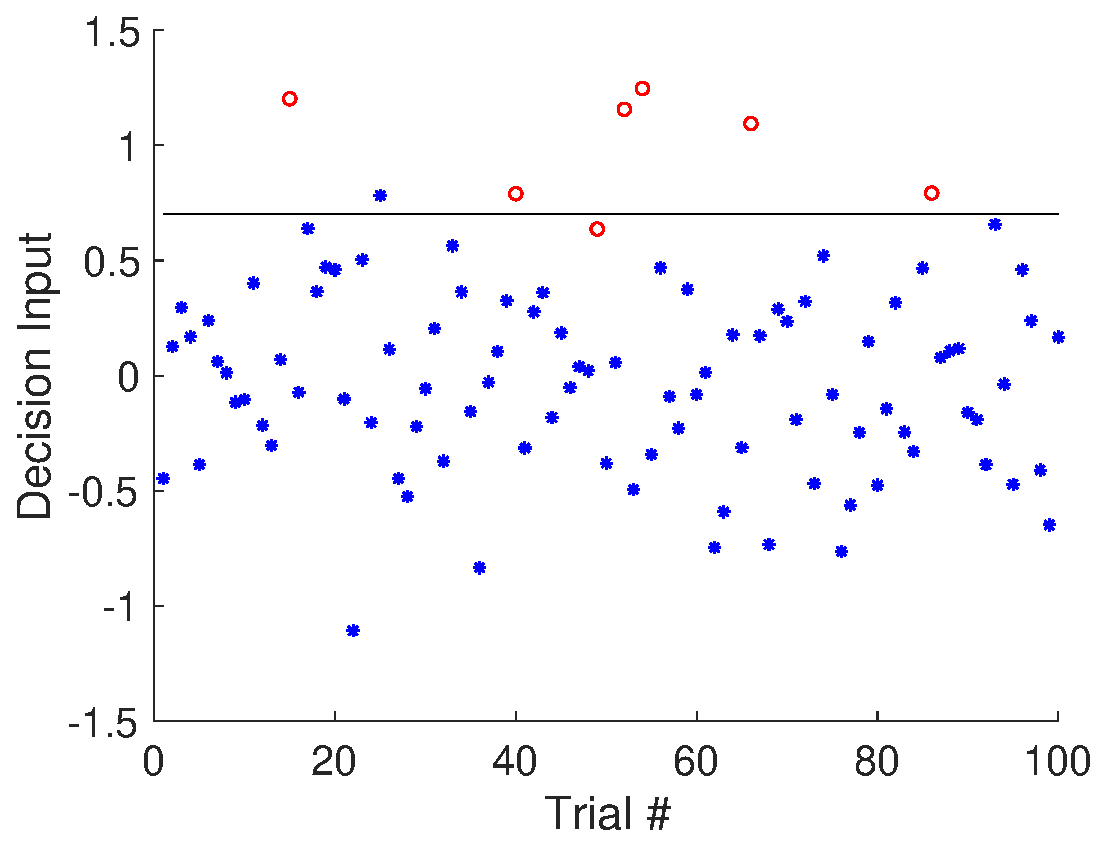
\includegraphics[width=2.4in]{../images/LectureActivitySymbolErrors.eps} }
    \caption{Activity example for threshold $= 0.7$, $a_0=0$, $a_1=1$, $\sigma_w=0.4$, $\PR{H_0}=0.9$, and 100 trials.  There are a total of 2 errors.}
    \label{F:LectureActivitySymbolErrors}
  \end{figure}


\section{Detection with Multiple Symbols}

When we only had $s_0(t)$ and $s_1(t)$, we saw that our decision was
based on which of the following was higher:
\[
  f_{X|H_0}(x| H_0) \PR{H_0} \quad \mbox{and} \quad f_{X|H_1}(x| H_1) \PR{H_1}
\]

For $M$-ary signals, we'll see that we need to consider the highest
of all $M$ possible events $H_m$,
\begin{eqnarray}
  H_0: && r(t) = s_0(t) + w(t) \nonumber \\
  H_1: && r(t) = s_1(t) + w(t) \nonumber \\
  \cdots && \cdots \nonumber \\
  H_{M-1}: && r(t) = s_M(t) + w(t) \nonumber
\end{eqnarray}
which have joint probabilities,
\begin{eqnarray}
  H_0: && f_{X|H_0}(x| H_0) \PR{H_0} \nonumber \\
  H_1: && f_{X|H_1}(x| H_1) \PR{H_1} \nonumber \\
  \cdots && \cdots \nonumber \\
  H_{M-1}: && f_{X|H_{M-1}}(x| H_{M-1}) \PR{H_{M-1}} \nonumber
\end{eqnarray}
A similar derivation to the one we did for binary 1-D Bayesian detection would show that the region $R_i$ in which it is optimal to decide $H_i$ is for all $X$ such that its joint probability is highest, that is,
\[
R_i = \left\{ X \mbox{ s.t. } f_{X|H_i}(x| H_i) \PR{H_i} > f_{X|H_j}(x| H_j) \PR{H_j} \mbox{ for all } j\neq i \right\}
\]

For this class, we'll usually consider the case of equally probable signals.  (While equi-probable signals is sometimes not the case for
$M=2$ binary detection, it is very rare in higher $M$ communication
systems because it is easy for communications systems designers to encode the data so that each symbol is equally likely to be transmitted.)  If $\PR{H_0} = \cdots = \PR{H_{M-1}}$ then we only need to find the $i$ that makes the likelihood $f_{X|H_i}(x| H_i)$ maximum, that is, maximum likelihood detection.
\[
  \mbox{Symbol Decision} = \arg \max_i f_{X|H_i}(x| H_i)
\]
For Gaussian (conditional) r.v.s with equal variances $\sigma_w^2$,
it is better to maximize the log of the likelihood rather than the likelihood directly, so
\[
  \log f_{X|H_i}(x| H_i) =  -\frac{1}{2}\log (2\pi \sigma_w^2)  - \frac{(x-a_i)^2}{2\sigma_w^2}
\]
This is maximized when $(x-a_i)^2$ is minimized.  Essentially, this
is a (squared) distance between $x$ and $a_i$.  So, the decision is,
find the $a_i$ which is closest to $x$.

The decision between two neighboring signal vectors $a_i$ and
$a_{i+1}$ will be
\[
 r  \decision{H_{i+1}}{H_i} \gamma_{i,i+1} = \frac{a_i + a_{i+1}}{2}
\]


As an example:  4-ary PAM.  See Figure
\ref{F:4AryPAM-DecisionThresholds}.

  \begin{figure}[htbp]
    \centerline{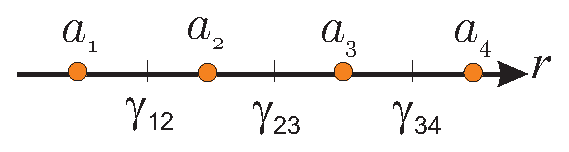
\includegraphics[width=2.4in]{../images/4AryPAM-DecisionThresholds.eps} }
    \caption{Signal space representation and decision thresholds for 4-ary PAM.}
    \label{F:4AryPAM-DecisionThresholds}
  \end{figure}


\section{Random Processes for Noise}

In order to study how noise affects communications receivers, we need to recall some background in the analysis of random processes.  A \emph{random process} $X(t)$ is a random function of continuous time $t$. (A \emph{random sequence} $X(n)$ is a sequence of random variables indexed by time index $n$.)  

The physics of thermal noise says that it has power spectral density that is approximately $kT_e$ where $k=1.3807\times 10^{23}$ J/K is Boltzmann's constant and $T_e$ is called the ``effective noise temperature'', which is proportional to the temperature of what the antenna is pointing at, and multiplied by a factor related to noise amplification within the receiver.  $T_e$ is a temperature in Kelvin.  This constant $kT_e$ is constant across the frequencies we use for communications system.  At room temperature, the power spectral density of thermal noise goes to zero at frequencies above $10^{13}$ Hz, that is, 10 Terahertz or 10,000 GHz.  This is orders of magnitude above frequencies at which most communications signals are sent.  The Rice book (4.5.2) has a good analysis of
the physics of thermal noise.  In short, the physics says that the PSD is flat in the bands we use, and that it is zero mean.

One of the most important and surprising results from random processes is that the autocorrelation function and the power spectral density are Fourier transform pairs, given certain conditions.  This helps us figure out how noise affects receivers, as we show next. 

\subsection{Autocorrelation and Power Spectral Density}


\Definition{Mean Function}{The mean function of the random
process $X(t)$ is 
\[
  \mu_X(t) = \E{}{X(t)}
\]
}
Note the mean is taken over all possible realizations of $X(t)$.  If you record one signal over all time $t$, you don't have anything to average to get the mean function $\mu_X(t)$.

\Definition{Autocorrelation Function}{ The autocorrelation function
of a random process $X(t)$ is
\[
  R_X(t, \tau) = \E{}{X(t) X(t - \tau)}
\]
The autocorrelation of a random sequence $X(n)$ is
\[
  R_X(n, k) = \E{}{X(n) X(n - k)}
\]
}

\Definition{Wide-sense stationary (WSS)}{ A random process is
wide-sense stationary (WSS) if
\begin{enumerate}
  \item $\mu_X = \mu_X(t) = \E{}{X(t)}$ is independent of $t$.
  \item $R_X(t, \tau)$ depends only on the time difference
  $\tau$ and not on $t$.  We then denote the
  autocorrelation function as $R_X(\tau)$.
\end{enumerate}
A random process is wide-sense stationary (WSS) if
\begin{enumerate}
  \item $\mu_X = \mu_X(n) = \E{}{X(n)}$ is independent of $n$.
  \item $R_X(n, k)$ depends only on $k$ and not on $n$.  We then denote the
  autocorrelation function as $R_X(k)$.
\end{enumerate}}
\textbf{The power of a signal is given by $R_X(0)$.}


\paragraph{Power Spectral Density}

The power spectral density $S_X(f)$ is a positive real-valued function equal to the density of power in a random process $X(t)$ near the frequency $f$.  It has units of Watts / Hz.  The (average) power between two frequencies $f_1$ and $f_2$ is the integral of $S_X(f)$ from $f_1 < f < f_2$. 

We know from random processes:  For a WSS random process $X(t)$ (and for a random
sequence $X(n)$) that its power spectral density can be computed as,
\begin{eqnarray}
  S_X(f) &=& \Fourier{R_X(\tau)} \nnn
  S_X(e^{j\Omega}) &=& \DTFT{R_X(k)} \nn
\end{eqnarray}

\Example{What is the autocorrelation function for thermal noise?}

We know from physics that thermal noise has constant power spectral density, and that the random process is WSS.  As Rice says ``for historical reasons this constant value is designated $N_0/2$''.  In this case, what is the autocorrelation function $R_w(\tau)$?

\Solution{
We're given $S_w(f) = N_0/2$.  The relationship is:
\[
S_X(f) = \Fourier{R_X(\tau)} 
\]
So 
\[
R_X(\tau) =\IFourier{S_X(f)} = \IFourier{N_0/2}
\]
But $N_0/2$ is just a constant.  Looking at a Fourier transform table, the solution is
\[
R_X(\tau) = \frac{N_0}{2} \delta (\tau).
\]
}

\subsection{Uncorrelated Noise}

A random sequence $X(n)$ is an \emph{uncorrelated noise} sequence if it is WSS and has autocorrelation function
\[
  R_X(k) = \E{}{X(n)X(n-k)} = \sigma^2 \delta(k)
\]
This says that each element of the sequence $X(n)$  is uncorrelated with $X(m), m\neq n$.

A random process $X(t)$ is an \emph{uncorrelated noise} random process if it is WSS and has autocorrelation function
\[
  R_X(\tau) = \E{}{X(t)X(t-\tau)} = \sigma^2 \delta(\tau)
\]
Again, this says that the value of $X(t)$  is uncorrelated with $X(t'), t'\neq t$.


This noise random process is referred to in textbooks as `white noise' because it has equal parts of every frequency (analogy to light).  But as I've mentioned before, black and gray also are constant in the frequency domain, so calling it `white' is arbitrary.  A more precise name is \emph{uncorrelated noise}.

Note that describing a random process / sequence as ``uncorrelated'' does NOT say that the distribution of its samples are Gaussian.  In order to specify that, we call it \emph{uncorrelated Gaussian noise}.  We typically model thermal noise as additive uncorrelated Gaussian noise (AUGN).  That is, it adds to the received signal.








\subsection{Noise in Correlation Receiver}

Previously, we had said that $r(t)$ was equal to the transmitted signal $s(t)$ plus noise:
\[
 r(t) = s(t) + w(t)
\]
As implied, we consider $w(t)$ to be uncorrelated and Gaussian with zero mean and PSD $S_W(f) = N_0/2$, or equivalently, $R_W(\tau) = N_0/2 \delta(\tau)$.  

What is the output of the correlation receiver?  Recall $x_k$ is defined as $\langle r(t), \phi_k(t) \rangle$, or
\begin{eqnarray}
  x_k &=& \int_{-\infty}^\infty r(t) \phi_k(t) dt
      \nonumber \\
    &=& \int_{-\infty}^\infty [s_i(t) + w(t)] \phi_k(t) dt
      \nonumber \\
    &=& a_{i,k} + \int_{-\infty}^\infty w(t) \phi_k(t) dt
      \nonumber \\
    &=& a_{i,k} + w_k
      \nonumber
\end{eqnarray}
where we define
\[
 w_k = \langle w(t), \phi_k \rangle = \int_{-\infty}^\infty w(t) \phi_k(t) dt.
\]

What can we know about $w_k$?  What are the mean and covariance of $\{w_k\}$?  For practice, prove that: 1) $w_k$ are all zero mean; and 2) the correlation of $w_k$ and $w_m$ is zero unless $k=m$, and in that case, is equal to $N_0/2$.  

\Solution{
First, $w_k$ is zero mean:
\[
  \E{}{w_k} = \int_{-\infty}^\infty \E{}{w(t)} \phi_k(t) dt = 0
\]
Next we can show that $w_1, \ldots, w_N$ are i.i.d. by calculating
the autocorrelation $R_w(m,k)$.
\begin{eqnarray}
  R_w(m,k) &=& \E{}{w_k w_m}
      \nonumber \\
    &=& \int_{t=-\infty}^\infty \int_{\tau=-\infty}^\infty \E{}{w(t) w(\tau)} \phi_k(t) \phi_m(\tau) d\tau dt
      \nonumber \\
    &=& \int_{t=-\infty}^\infty \int_{\tau=-\infty}^\infty \frac{N_0}{2}\delta(t-\tau) \phi_k(t) \phi_m(\tau) d\tau dt
      \nonumber \\
    &=& \frac{N_0}{2} \int_{t=-\infty}^\infty \phi_k(t) \phi_m(t) dt
      \nonumber \\
    &=& \frac{N_0}{2} \delta(k-m) = \pdfarray{\frac{N_0}{2}}{m=k}
      \nonumber
\end{eqnarray}
}

Is $w_k$ Gaussian?  Yes -- an integral is a linear operation, and any linear function of a Gaussian random process is also Gaussian.  

Are $\{w_k\}$ independent?  Yes -- for Gaussian random variables, a covariance of zero implies independent.  

Since the noise components are independent, then $x_k$ (the sum of $a_{i,k}$ and $w_k$) are also
Gaussian and independent. Why? Because $a_{i,k}$ is a deterministic constant, and thus $x_k$ are Gaussian with mean $a_{i,k}$.  But that change in mean doesn't change the autocovariance function. 

What is the pdf of $\mbx = [x_0, \ldots, x_K]^T$?

\Solution{ 
\[
 f_{X_k}(x_k) = \frac{1}{\sqrt{2\pi (N_0/2)}} e^{-\frac{(x_k - a_{i,k})^2}{2(N_0/2)}}
\]
And, since the $\{x_k\}$ are independent, the joint pdf of all of them is the product of the marginal pdfs:
\begin{eqnarray}
 f_{\mbx}(\mbx) &=& \prod_{k=1}^K f_{X_k}(x_k) \nonumber \\
   &=& \prod_{k=1}^K \frac{1}{\sqrt{2\pi (N_0/2)}} e^{-\frac{(x_k - a_{i,k})^2}{2(N_0/2)}}
     \nonumber \\
   &=& \frac{1}{[2\pi (N_0/2)]^{K/2}} e^{-\frac{\sum_{k=1}^K (x_k - a_{i,k})^2}{2(N_0/2)}}
     \nonumber
\end{eqnarray}
}

\subsection{Gaussian Random Vectors}

\Definition{Multivariate Gaussian R.V.}{An $n$-length R.V. $\mbX$
is multivariate Gaussian with mean $\mu_\mbX$,  and covariance
matrix $C_\mbX$ if it has the pdf,
\[
f_\mbX(\mbx) = \frac{1}{\sqrt{(2\pi)^n \mbox{det}(C_\mbX)}}
  \exp \left[ -\frac{1}{2}(\mbx-\mu_\mbX)^T  C_\mbX^{-1}
  (\mbx-\mu_\mbX) \right]
\]
where $\mbox{det}()$ is the determinant of the covariance matrix, and
$C_\mbX^{-1}$ is the inverse of the covariance matrix. }

\textbf{Any linear combination of jointly Gaussian random variables
is another jointly Gaussian random variable.}  For example, if we
have a matrix $A$ and we let a new random vector $\mbY = A \mbX$,
then $\mbY$ is also a Gaussian random vector with mean $A\mu_\mbX$
and covariance matrix $A C_\mbX A^T$.

If the elements of $\mbX$ were independent random variables, the pdf
would be the product of the individual pdfs (as with any random
vector) and in this case the pdf would be:
\[
f_\mbX(\mbx) = \frac{1}{\sqrt{(2\pi)^n \prod_i \sigma_i^2}}
  \exp \left[ -\sum_{i=1}^n \frac{(x_i-\mu_{X_i})^2}{2\sigma_{X_i}^2}  \right]
\]

Section 4.3 spends some time with 2-D Gaussian random vectors, which
is the dimension with which we spend most of our time in this class.


 \clearpage

\StartOf{Lecture 11}

\Today{(0) Noise (Notes from Lecture 10); (1) $N$-dim Bayesian Detection Theory}

\announcements{
\begin{itemize}
\item Reading: Today: Rice 6.1, 6.2, Wed: No new reading
\item Project 3 due today at 11:59pm
\item HW 5 due Wed. I will post solutions Thu at midnight so that you can study. 
\item Exam 1 is Mar 2 (one week from today) in class. Exam 1 study material is on Canvas under Pages: View All Pages: Exam 1 Practice.  
\end{itemize}
}

\section{$M$-ary Detection Theory in $N$-dimensional signal space}

We are going to start to talk about QAM, PSK, and FSK, modulations with two dimensional signal vectors. We also consider in this course modulations with higher dimensional signal vectors.  We have developed $M$-ary detection theory for 1-D signal vectors, and now we will extend that to $N$-dimensional signal vectors.

Setup:
\begin{itemize}
 \item Transmit: one of $M$ possible symbols, $\mba_0, \ldots, \mba_{M-1}$.  These vectors are length $N$.
 \item Receive: the symbol plus noise:
\begin{eqnarray}
  H_0: && \mbX = \mba_0 + \mbn \nonumber \\
  \cdots && \cdots \nonumber \\
  H_{M-1}: && \mbX = \mba_{M-1} + \mbn \nonumber
\end{eqnarray}
 \item Assume: $\mbn$ is multivariate Gaussian, each component $n_i$ is independent with zero mean and variance $\sigma_N^2 = N_0/2$.
 \item Assume: Symbols are equally likely.
 \item Question: What are the optimal decision regions?
\end{itemize}

When symbols are equally likely, the optimal decision turns out to be given by the maximum likelihood receiver,
\begin{equation} \label{E:NDimML}
  \hat{i} = \argmax{i} \log f_{\mbX|H_i}(\mbx|H_i)
\end{equation}
Here,
\[
 f_{\mbX|H_i}(\mbx|H_i) = \frac{1}{\sqrt{(2\pi)^{N} \mbox{det}(C_\mbX)} } \exp \left[ -\frac{1}{2}(\mbx-\mba_i)^T  C_\mbX^{-1}
  (\mbx-\mba_i) \right].
\]
But as we derived earlier, the elements of vector $\mbx$ are uncorrelated and each have the same variance $\sigma_N^2$.  This means that 
\[
 f_{\mbX|H_i}(\mbx|H_i) = \frac{1}{(2\pi\sigma_N^2)^{N/2} } \exp \left[ - \sum_{i=0}^{N-1} \frac{(x_k - a_{i,k} )^2 }{2\sigma_N^2} \right]
\]
or
\[
 f_{\mbX|H_i}(\mbx|H_i) = \frac{1}{(2\pi\sigma_N^2)^{N/2} } \exp \left[ - \frac{\|\mbx - \mba_{i}\|^2 }{2\sigma_N^2} \right]
\]
So when we want to solve (\ref{E:NDimML}) we can simplify quickly to:
\begin{eqnarray}
   \hat{i} &=& \argmax{i} \left\{ \log \frac{1}{(2\pi\sigma_N^2)^{N/2} }  -\frac{\|\mbx - \mba_i \|^2 }{2\sigma_N^2} \right\}
   \nnn
   \hat{i} &=& \argmax{i} - \frac{\|\mbx - \mba_i \|^2 }{2\sigma_N^2}
   \nnn
   \hat{i} &=& \argmin{i} \|\mbx - \mba_i \|^2 
   \nnn
   \hat{i} &=& \argmin{i} \|\mbx - \mba_i \|
\end{eqnarray}
Again:  Just find the $\mba_i$ in the signal space diagram which is
closest to $\mbx$.

\subsection{Pairwise Comparisons}

When is $\mbx$ closer to $\mba_i$ than to $\mba_j$ for some other
signal space point $j$? Solution: \textbf{The two decision regions
are separated by a straight line} (Note: replace ``line'' with plane
in 3-D, or subspace in $N$-D).  To find this line:
\begin{enumerate}
  \item Draw a line segment connecting $\mba_i$ and $\mba_j$.
  \item Draw a point in the middle of that line segment.
  \item Draw the perpendicular bisector of the line segment through
  that point.
\end{enumerate}

\Example{ Derive a formula for the dividing line (dividing plane when $N>2$) between $\mba_i$ and $\mba_j$ for $j\neq i$ when symbols are equally likely.}

\Solution{
 Try to find the locus of points $\mbx$ which satisfy the equality of distances between the two symbol points:
\[
  \| \mbx - \mba_i \|^2 = \| \mbx - \mba_j \|^2
\]
You can do this by using the inner product to represent the
magnitude squared operator:
\[
  (\mbx - \mba_i)^T(\mbx - \mba_i) =(\mbx - \mba_j)^T(\mbx - \mba_j)
\]
Then use FOIL (multiply out), cancel, and reorganize to find a
linear equation in terms of $\mbx$.  This is left as an exercise.}



\subsection{Decision Regions}
Each pairwise comparison results in a linear division of space (a half-space).  The
combined decision region, the intersection of all of these of half-spaces, $R_i$, is the space which in which all conditions are satisfied.  This intersection space is where $\mba_i$ is the closest symbol out of all of the $M$ symbols.

A diagram of all of the decision regions is called a Voronoi diagram.

\Example{Optimal Decision Regions} 

We will do an activity in class to draw the decision regions for Bayesian detection for a 2D constellation diagram.  See Figure \ref{F:DetectionRegionsExample} for two randomly generated constellations with $M=5$.

\begin{figure}[htbp]
  \centerline{(a) 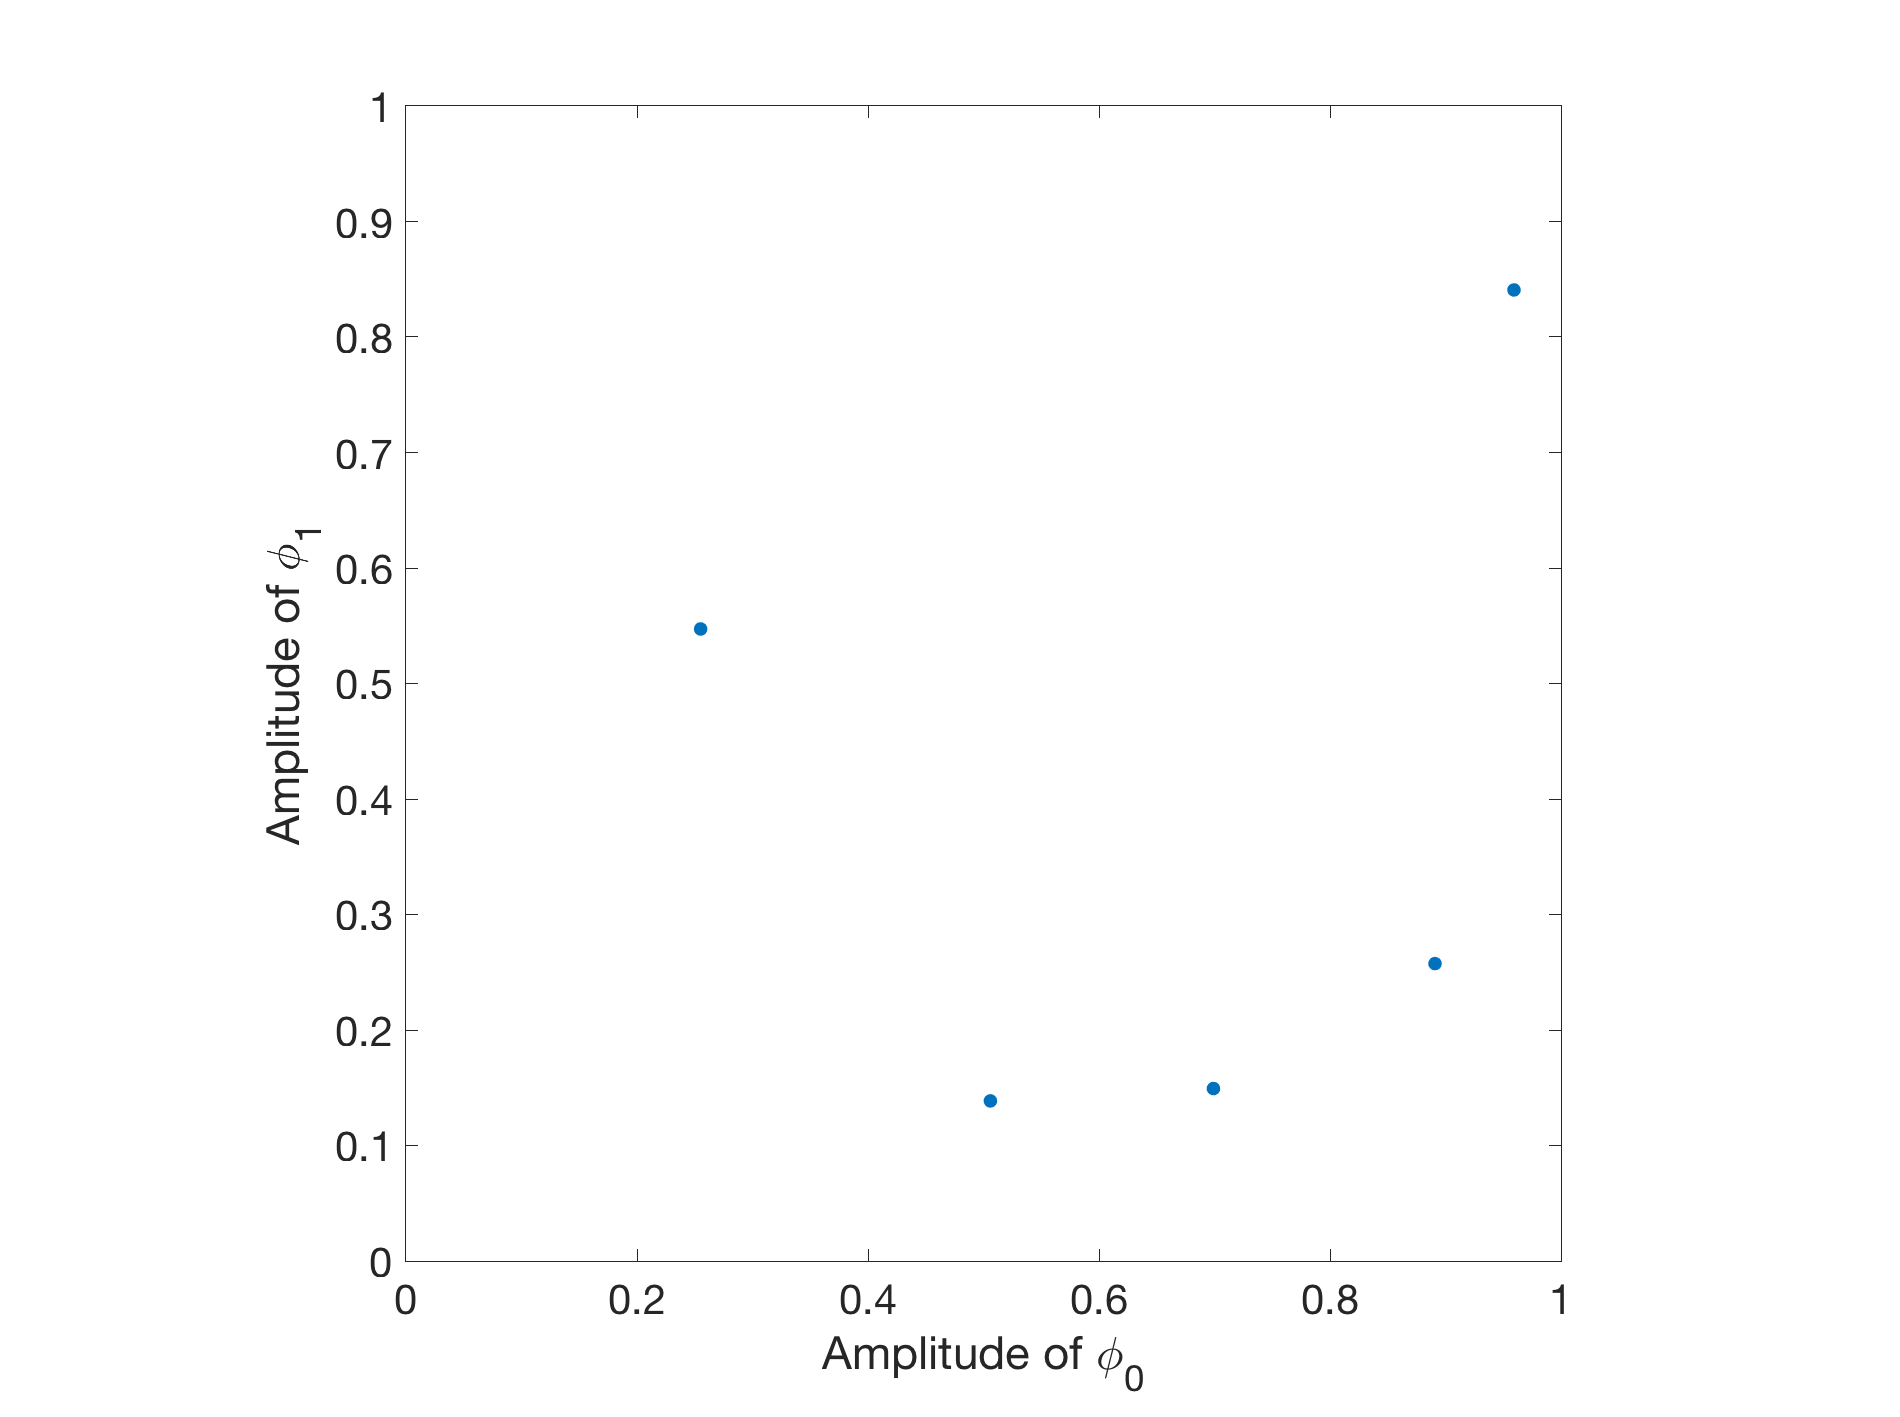
\includegraphics[width=0.9\textwidth]{../images/ExampleVoronoiDiagram_1.png}}
\centerline{  (b) 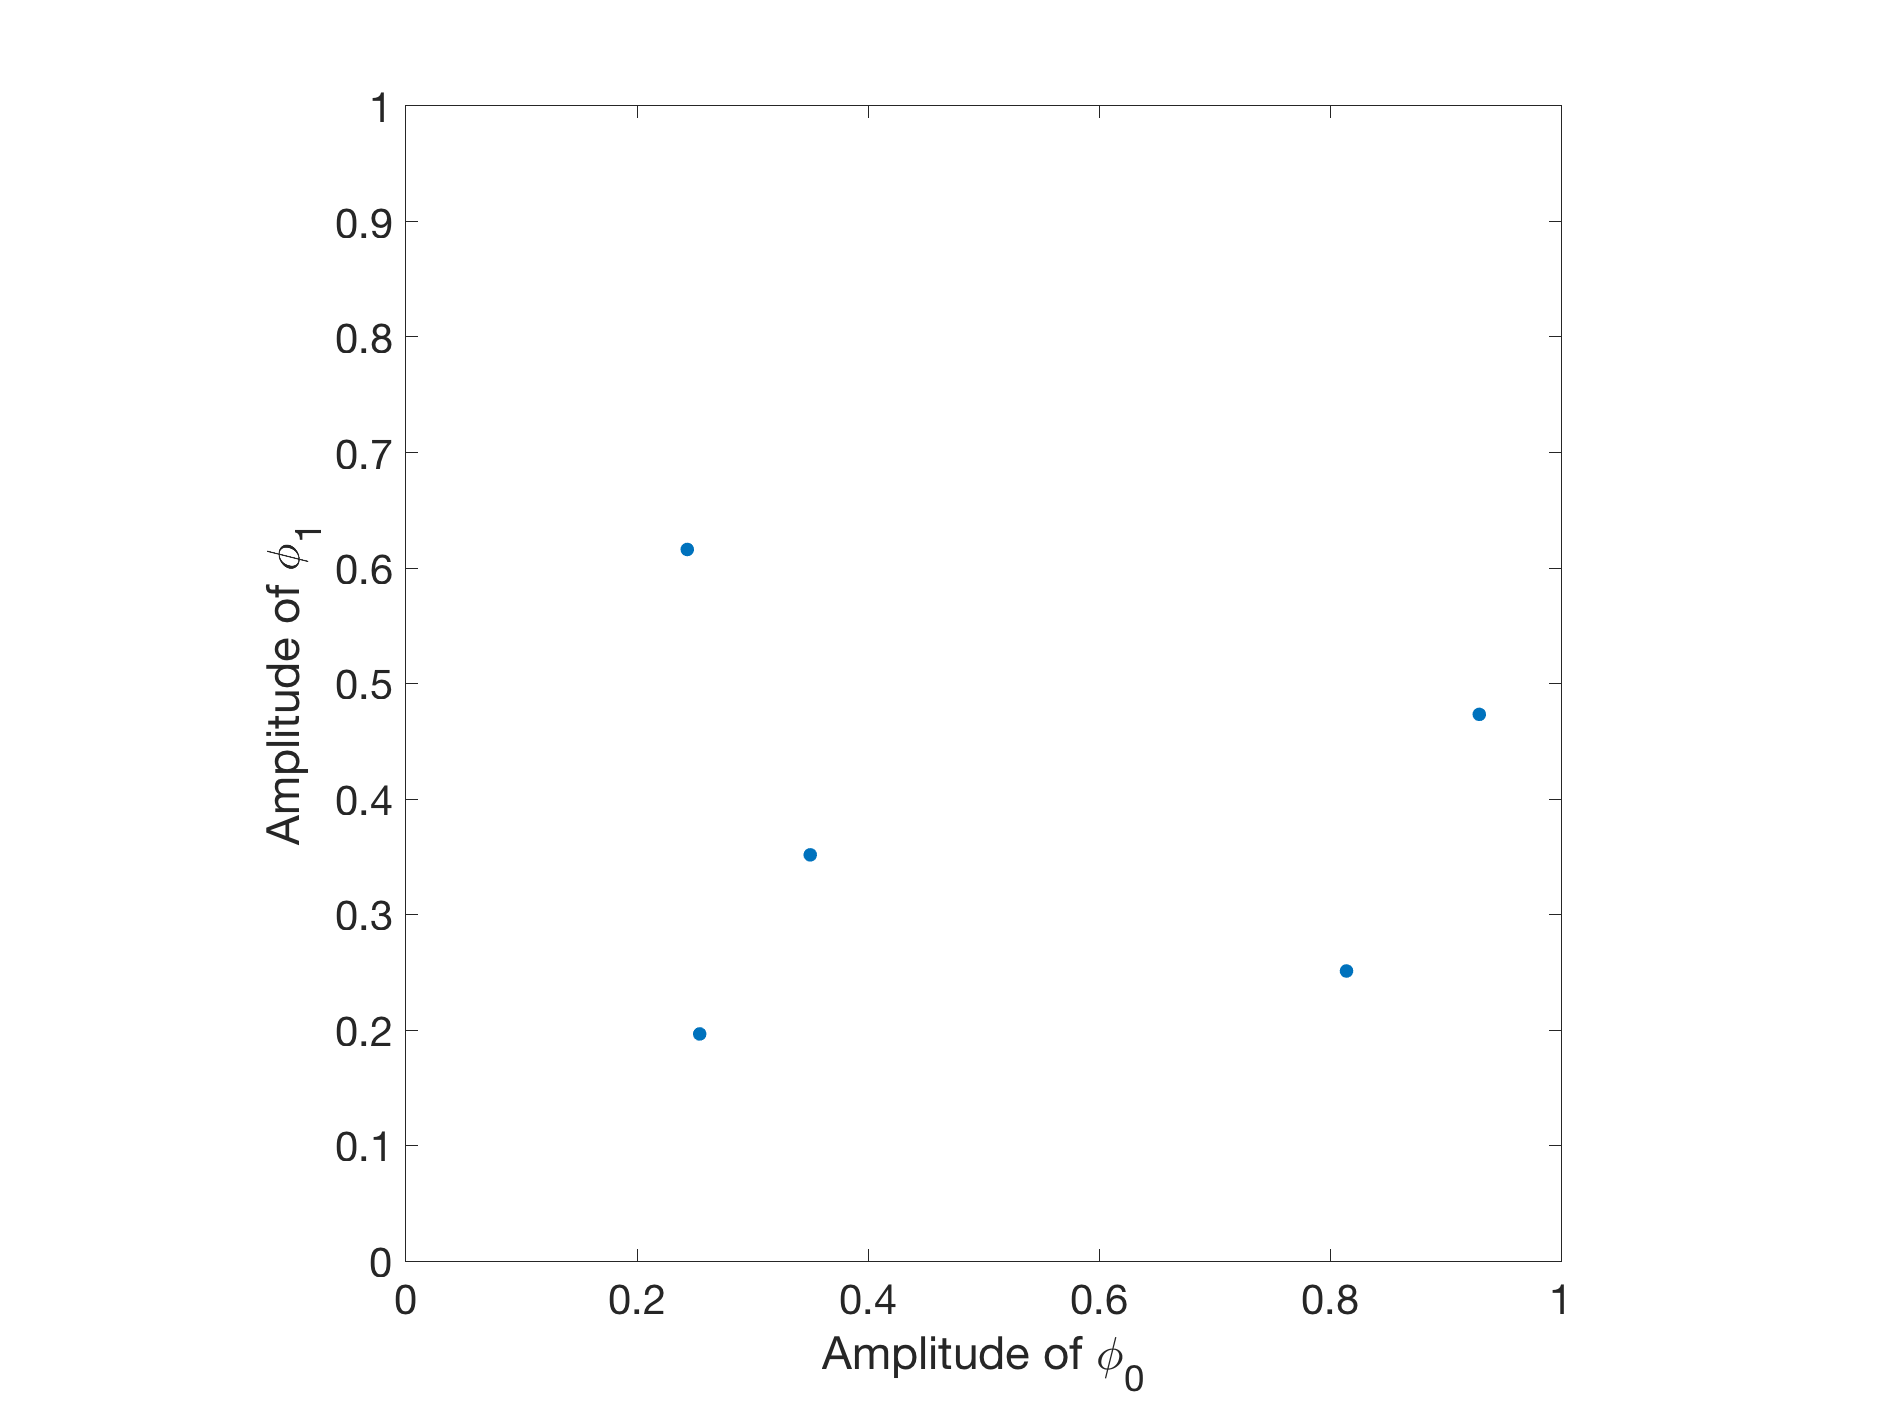
\includegraphics[width=0.9\textwidth]{../images/ExampleVoronoiDiagram.png}}
  \caption{Example signal space diagrams.  Draw the optimal decision regions.}
  \label{F:DetectionRegionsExample}
\end{figure}



\subsection{Symbol Distances}

We mentioned, when talking about signal space diagrams, a distance between vectors,
\[
 d_{i,j} = \| \mba_i - \mba_j \| = \left[ \sum_{k=1}^M (a_{i,k} -
 a_{j,k})^2 \right]^{1/2}
\]
In general we will start to use these distances quite often in the analysis of a modulation method.


\StartOf{Lecture 12}

\Today{ (1) Probability of Error in $M$-ary PAM}

\announcements{
\begin{itemize}
  \item Today:  Rice 6.1; Wed 3/4: Rice 6.2.
  \item Office Hours for Keren Li: 4-5pm today.  Neal: Friday 9:15am-10:15am
  \item Homework 5 due today
  \item Exam 1 on Monday 3/2 in class
  \item Project 4 due Wed 3/4
\end{itemize}
}




\section{Review of $N$-D Detection Theory with Multiple Symbols}

For $M$-ary signals, we discussed how the lowest probability of error, or \emph{Bayesian optimal}, detector finds the maximum joint probability, among the $M$ possible hypotheses $H_m$, for $m=1, \ldots, M$:
\begin{eqnarray}
  H_0: && f_{X|H_0}(x| H_0) \PR{H_0} \nonumber \\
  H_1: && f_{X|H_1}(x| H_1) \PR{H_1} \nonumber \\
  \cdots && \cdots \nonumber \\
  H_{M-1}: && f_{X|H_{M-1}}(x| H_{M-1}) \PR{H_{M-1}} \nonumber
\end{eqnarray}
The receiver finds which of these joint probabilities is highest.  For equally probable
symbols, additive Gaussian noise with identical variance in each $H_m$,
\[
  \mbox{Symbol Decision} = \arg \max_i \| \mbx - \mba_i \|
\]


\section{$M$-ary PAM Probability of Error}

\begin{figure}[htbp]
  \centerline{ 


\tikzset{every picture/.style={line width=0.75pt}} %set default line width to 0.75pt        

\begin{tikzpicture}[x=0.75pt,y=0.75pt,yscale=-1,xscale=1]
%uncomment if require: \path (0,300); %set diagram left start at 0, and has height of 300

%Straight Lines [id:da0785677110363594] 
\draw    (173.96,114) -- (507.96,114) ;
\draw [shift={(509.96,114)}, rotate = 180] [color={rgb, 255:red, 0; green, 0; blue, 0 }  ][line width=0.75]    (10.93,-3.29) .. controls (6.95,-1.4) and (3.31,-0.3) .. (0,0) .. controls (3.31,0.3) and (6.95,1.4) .. (10.93,3.29)   ;

%Shape: Circle [id:dp8429373004294252] 
\draw  [fill={rgb, 255:red, 208; green, 2; blue, 27 }  ,fill opacity=1 ] (306,114.48) .. controls (306,112.01) and (308.01,110) .. (310.48,110) .. controls (312.96,110) and (314.96,112.01) .. (314.96,114.48) .. controls (314.96,116.96) and (312.96,118.96) .. (310.48,118.96) .. controls (308.01,118.96) and (306,116.96) .. (306,114.48) -- cycle ;
%Straight Lines [id:da9917337286598218] 
\draw    (330.96,107.29) -- (330.96,121.29) ;


%Shape: Circle [id:dp31317929420387847] 
\draw  [fill={rgb, 255:red, 208; green, 2; blue, 27 }  ,fill opacity=1 ] (266,114.48) .. controls (266,112.01) and (268.01,110) .. (270.48,110) .. controls (272.96,110) and (274.96,112.01) .. (274.96,114.48) .. controls (274.96,116.96) and (272.96,118.96) .. (270.48,118.96) .. controls (268.01,118.96) and (266,116.96) .. (266,114.48) -- cycle ;
%Shape: Circle [id:dp8703696009425539] 
\draw  [fill={rgb, 255:red, 208; green, 2; blue, 27 }  ,fill opacity=1 ] (227,114.48) .. controls (227,112.01) and (229.01,110) .. (231.48,110) .. controls (233.96,110) and (235.96,112.01) .. (235.96,114.48) .. controls (235.96,116.96) and (233.96,118.96) .. (231.48,118.96) .. controls (229.01,118.96) and (227,116.96) .. (227,114.48) -- cycle ;
%Shape: Circle [id:dp48312291319442124] 
\draw  [fill={rgb, 255:red, 208; green, 2; blue, 27 }  ,fill opacity=1 ] (186,114.48) .. controls (186,112.01) and (188.01,110) .. (190.48,110) .. controls (192.96,110) and (194.96,112.01) .. (194.96,114.48) .. controls (194.96,116.96) and (192.96,118.96) .. (190.48,118.96) .. controls (188.01,118.96) and (186,116.96) .. (186,114.48) -- cycle ;
%Shape: Circle [id:dp32010417887626774] 
\draw  [fill={rgb, 255:red, 208; green, 2; blue, 27 }  ,fill opacity=1 ] (467,113.48) .. controls (467,111.01) and (469.01,109) .. (471.48,109) .. controls (473.96,109) and (475.96,111.01) .. (475.96,113.48) .. controls (475.96,115.96) and (473.96,117.96) .. (471.48,117.96) .. controls (469.01,117.96) and (467,115.96) .. (467,113.48) -- cycle ;
%Shape: Circle [id:dp665622950437736] 
\draw  [fill={rgb, 255:red, 208; green, 2; blue, 27 }  ,fill opacity=1 ] (425,113.48) .. controls (425,111.01) and (427.01,109) .. (429.48,109) .. controls (431.96,109) and (433.96,111.01) .. (433.96,113.48) .. controls (433.96,115.96) and (431.96,117.96) .. (429.48,117.96) .. controls (427.01,117.96) and (425,115.96) .. (425,113.48) -- cycle ;
%Shape: Circle [id:dp5860873971209044] 
\draw  [fill={rgb, 255:red, 208; green, 2; blue, 27 }  ,fill opacity=1 ] (387,113.48) .. controls (387,111.01) and (389.01,109) .. (391.48,109) .. controls (393.96,109) and (395.96,111.01) .. (395.96,113.48) .. controls (395.96,115.96) and (393.96,117.96) .. (391.48,117.96) .. controls (389.01,117.96) and (387,115.96) .. (387,113.48) -- cycle ;
%Shape: Circle [id:dp20437801267978872] 
\draw  [fill={rgb, 255:red, 208; green, 2; blue, 27 }  ,fill opacity=1 ] (346,113.48) .. controls (346,111.01) and (348.01,109) .. (350.48,109) .. controls (352.96,109) and (354.96,111.01) .. (354.96,113.48) .. controls (354.96,115.96) and (352.96,117.96) .. (350.48,117.96) .. controls (348.01,117.96) and (346,115.96) .. (346,113.48) -- cycle ;
%Straight Lines [id:da51291390000777] 
\draw    (370.96,108.29) -- (370.96,122.29) ;


%Straight Lines [id:da2811648906641422] 
\draw    (410.96,108.29) -- (410.96,122.29) ;


%Straight Lines [id:da4403380546942397] 
\draw    (450.96,107.29) -- (450.96,121.29) ;


%Straight Lines [id:da9495765085027235] 
\draw    (213.96,107.29) -- (213.96,121.29) ;


%Straight Lines [id:da24674873474006298] 
\draw    (253.96,107.29) -- (253.96,121.29) ;


%Straight Lines [id:da44203695518931974] 
\draw    (293.96,106.29) -- (293.96,120.29) ;



% Text Node
\draw (331.48,136.96) node   {$0$};
% Text Node
\draw (120,142) node   {$$};
% Text Node
\draw (191,93) node   {$\mathbf{a}_{0}$};
% Text Node
\draw (232,93) node   {$\mathbf{a}_{1}$};
% Text Node
\draw (270,93) node   {$\mathbf{a}_{2}$};
% Text Node
\draw (311,93) node   {$\mathbf{a}_{3}$};
% Text Node
\draw (351,94) node   {$\mathbf{a}_{4}$};
% Text Node
\draw (392,94) node   {$\mathbf{a}_{5}$};
% Text Node
\draw (430,94) node   {$\mathbf{a}_{6}$};
% Text Node
\draw (471,94) node   {$\mathbf{a}_{7}$};
% Text Node
\draw (187,72.5) node   {$-7A$};
% Text Node
\draw (227,74) node   {$-5A$};
% Text Node
\draw (266,74) node   {$-3A$};
% Text Node
\draw (307,74) node   {$-A$};
% Text Node
\draw (350,74) node   {$A$};
% Text Node
\draw (392,74) node   {$3A$};
% Text Node
\draw (430,74) node   {$5A$};
% Text Node
\draw (471,74) node   {$7A$};
% Text Node
\draw (372.48,136.96) node   {$2A$};
% Text Node
\draw (411.48,136.96) node   {$4A$};
% Text Node
\draw (452.48,136.96) node   {$6A$};
% Text Node
\draw (211.48,136.96) node   {$-6A$};
% Text Node
\draw (252.48,136.96) node   {$-4A$};
% Text Node
\draw (291.48,136.96) node   {$-2A$};


\end{tikzpicture}

}
  \caption{Signal space diagrams for 8-PAM, with optimal detection thresholds.}
  \label{F:8PAM_detection_thresholds}
\end{figure}

Consider $M$-PAM.  Our goal in this section is to find a formula for the probability that our optimal receiver makes a symbol error when receiving.

\subsection{Symbol Error}

The probability that we don't get the symbol correct is the
probability that $x$ does not fall within the range between the
thresholds in which it belongs.  Here, each $\mba_i = -7A + i(2A)$.  Also the
noise $\sigma_W^2 = N_0/2$, as described in our lecture on thermal noise.

Let's consider symbol $i=1$.  Recall $\mba_1 = -5A$.  The probability of error is the sum of the probability of deciding $H_0$, plus the probability of deciding $H_i$ for $i=2, \ldots, 7$.  That is, that the $x$ value is below $-6A$, or above $-4A$.  Thus
\begin{eqnarray}
  P(\mbox{symbol error}| H_1) 
    &=& \Q{\frac{-5A - (-6A) }{\sqrt{N_0/2}}} + \Q{\frac{-4A - (-5A) }{\sqrt{N_0/2}}}
  \nnn 
    &=& 2 \Q{\frac{A }{\sqrt{N_0/2}}}.
\end{eqnarray}

Assuming neighboring symbols $a_i$ are spaced by $2A$, the decision
threshold is always $A$ away from the symbol values. For the symbols
$i$ in the `middle',
\[
  P(\mbox{symbol error}| H_i) = 2 \Q{\frac{A }{\sqrt{N_0/2}}}
\]
For the symbols $i$ on the `sides',
\[
  P(\mbox{symbol error}| H_i) = \Q{\frac{A }{\sqrt{N_0/2}}}
\]
Since each symbol $H_i$ is equally likely, the overall probability of symbol error is the average of the conditional probabilities of symbol error.  That is:
\[
  P(\mbox{symbol error}) = \frac{1}{M} \sum_{i=0}^{M-1} P(\mbox{symbol error}| H_i)
\]
So overall,
\[
  P(\mbox{symbol error}) = \frac{2(M-1)}{M} \Q{\frac{A }{\sqrt{N_0/2}}}
\]

\noindent {\bf Symbol Error Rate and Average Bit Energy}:

How does this relate to the average bit energy $\En_b$?  We calculated in an earlier lecture the average symbol error for $M$-PAM as
\[
\En_s = \frac{(M^2-1)}{3} A^2
\]
But there are $\log_2 M$ bits per symbol.  We're going to want to express energy per bit instead of average energy per symbol.  Thus we use $\En_b$ to denote the average energy per bit.  Thus
\begin{equation}
\En_b = \frac{1}{\log_2 M} \frac{(M^2-1)}{3} A^2,    
\end{equation}
which means that
\[
A  = \sqrt{\frac{3 \log_2 M}{M^2-1}} \En_b
\]
So
\begin{equation} \label{E:PrSymbolErrorMPAM2}
  P(\mbox{symbol error}) = \frac{2(M-1)}{M} \Q{\sqrt{\frac{6 \log_2 M}{M^2-1} \frac{\En_b}{N_0}}}
\end{equation}
Equation (\ref{E:PrSymbolErrorMPAM2}) is plotted in Figure
\ref{F:plotPerrorMaryPAM}.

  \begin{figure}[htbp]
    \centerline{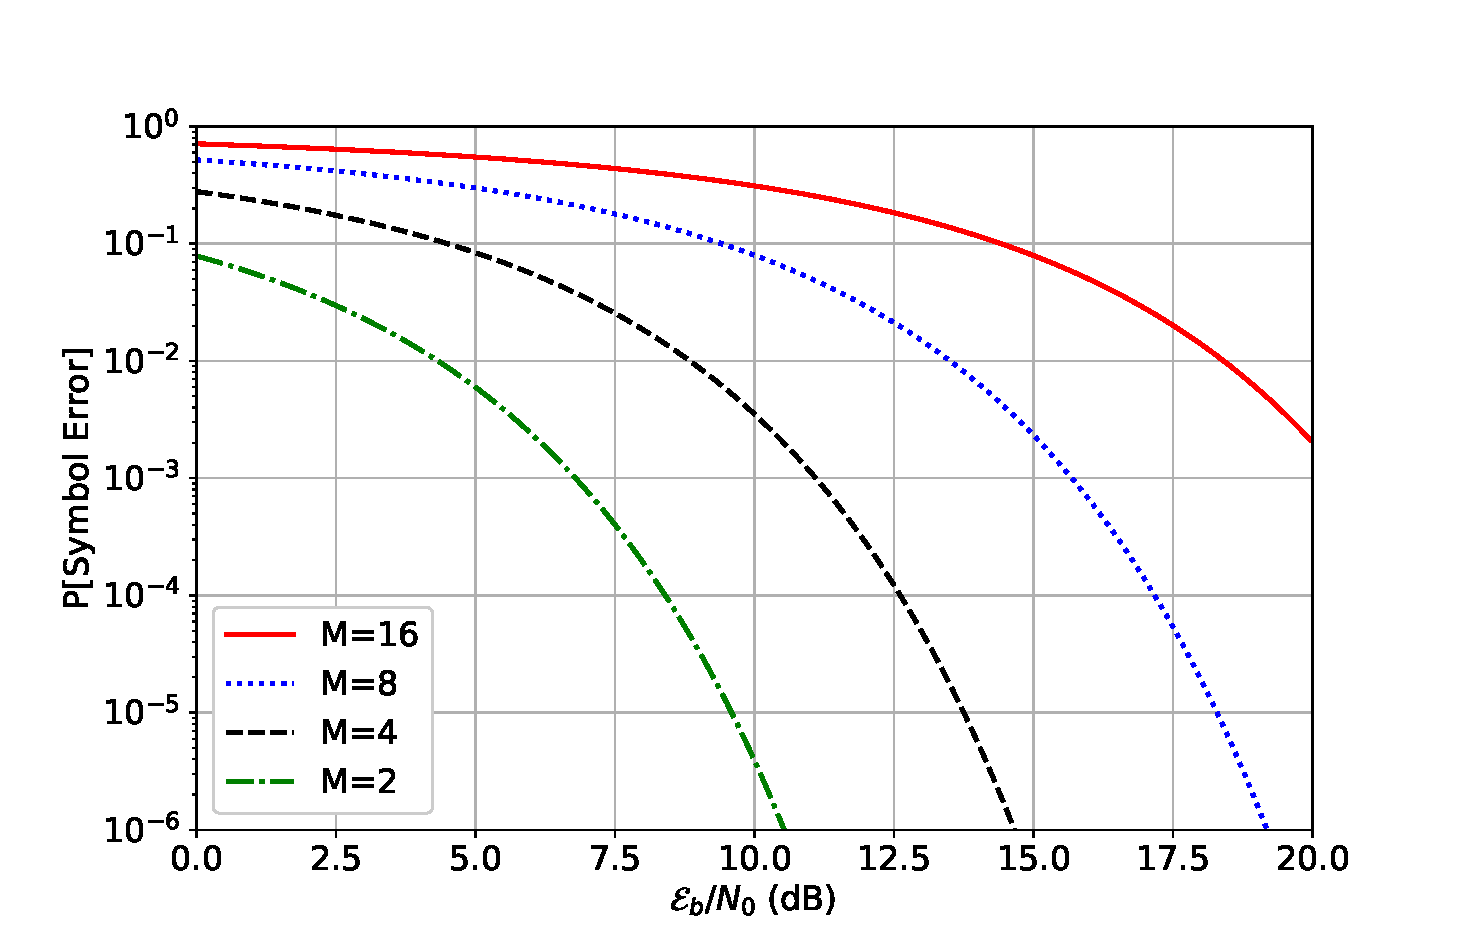
\includegraphics[width=\textwidth]{../images/plotPrSymbolErrorMPAM.eps} }
    \caption{Probability of Symbol Error in $M$-ary PAM.}
    \label{F:plotPerrorMaryPAM}
  \end{figure}


\subsection{Bit Errors and Gray Encoding}

For binary PAM, there are only two symbols, one will be assigned
binary 0 and the other binary 1.  When you make one symbol error
(decide $H_0$ or $H_1$ in error) then it will cause one bit error.

For $M$-ary PAM, bits and symbols are not synonymous.  Instead, we
carefully assign bit codes to symbols $1 \ldots M$ so that the most common receiver errors cause only one bit to be in error, and let less common receiver errors to cause more than one bit error.

\Example{Bit coding of $M=4$ symbols}  While the two options shown
in Figure \ref{F:4AryPAM-BitCodingOptions} both assign 2-bits to
each symbol in unique ways, one will lead to a higher bit error rate
than the other.  Is one is better or worse?
  \begin{figure}[htbp]
    \centerline{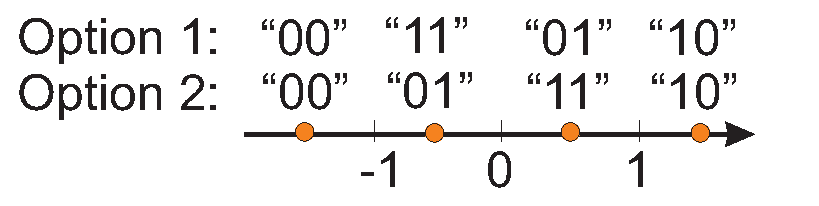
\includegraphics[width=0.5\textwidth]{../images/4AryPAM-BitCodingOptions.eps} }
    \caption{Two options for assigning bits to symbols in 4-PAM.}
    \label{F:4AryPAM-BitCodingOptions}
  \end{figure}

The key is to recall the model for noise.  It will not shift a
signal uniformly across symbols.  It will tend to leave the received
signal $x$ close to the original signal $a_i$.  The neighbors of
$a_i$ will be more likely than distant signal space vectors.

Thus Gray encoding will only change one bit across boundaries, as in
Option 2 in Figure \ref{F:4AryPAM-BitCodingOptions}.

\Example{Bit coding of $M=8$ symbols}  Assign three bits to each
symbol such that any two nearest neighbors are different in only one
bit (Gray encoding).

\Solution{Here is one solution.
  \begin{figure}[htbp]
    \centerline{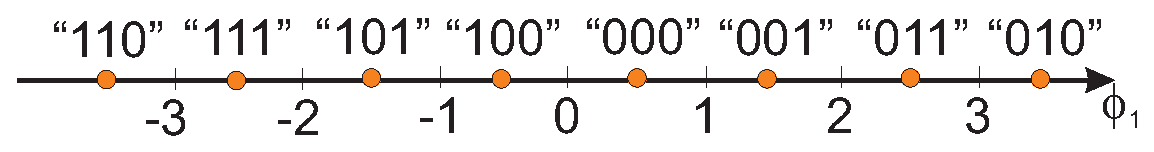
\includegraphics[width=0.6\textwidth]{../images/8AryPAM-GrayCoding.eps} }
    \caption{Gray encoding for 8-PAM.}
    \label{F:8AryPAM-GrayCoding}
  \end{figure}
}

\subsubsection{Bit Error Probabilities}

How many bit errors are caused by a symbol error in $M$-ary PAM?
\begin{itemize}
  \item One.  If Gray encoding is used, the errors will tend to be
  just one bit flipped, more than multiple bits flipped.  At least
  at high $\En_b/N_0$,
  \begin{equation} \label{E:PrBitErrorInGeneral}
    P(\mbox{error}) \approx \frac{1}{\log_2 M} P(\mbox{symbol error})
  \end{equation}
  \item Maybe more, up to $\log_2 M$ in the worst case.  Then, we
  need to study further the probability that $x$ will jump more than one decision
  region.
\end{itemize}
Generally, we study digital communications systems with high reliability, and high $\En_b/N_0$.  Thus when we calculate bit error rate for $M$-ary PAM, we
use (\ref{E:PrBitErrorInGeneral}).  We will show that this approximation is very good, in almost all cases for $M$-PAM and most common QAM/PSK modulations.  We will also discuss some particular examples in multi-dimensional signalling when this is not a great approximation.

Thus for $M$-PAM:
\begin{equation} \label{E:PrBitErrorMPAM2}
  P(\mbox{bit error}) \approx \frac{2(M-1)}{M \log_2 M} \Q{\sqrt{\frac{6 \log_2 M}{M^2-1} \frac{\En_b}{N_0}}}
\end{equation}


\section{Square QAM Probability of Error}

%This section is meant to introduce the problems we'll have as we compute the probability of symbol error in QAM and PSK, and in general, for higher dimensional symbol space diagrams.  

Consider now QAM modulation, in general, which is $N=2$.
Recall that our symbol decision is  $\arg \max_i \| \mbx - \mba_i \|$, and that this creates decision regions using a Voronoi diagram.  This can, in general, be quite complicated because we'd have a probability of error that is an integral of a 2-D Gaussian pdf in the area outside of some polygon containing $\mba_i$.  Two dimensional integrals of a Gaussian pdf aren't something for which we can find an analytical solution.  While we can solve numerically for such integrals, and people do, we tend to find easier approximations whenever possible.

Square QAM is an example where we can make the probability of symbol error formula exact, and analytical.  To do this, consider square $M$-QAM as two orthogonal $\sqrt{M}$-PAM systems.  In this case, the bits of each symbol are separated into first the bits corresponding to the in-phase component of the modulation, and next the bits corresponding to the quadrature component.  We can see that using gray coding in each component, we can arrange it so that the first bits are completely dependent on the in-phase component.  Because these $\log_2 \sqrt{M}$ bits are independent of the quadrature, the probability of bit error for these bits is the same as the the probability of bit error for $\sqrt{M}$-PAM.  Similarly, the next $\log_2 \sqrt{M}$ bits are independent of the in-phase component, and thus the probability of bit error for these bits is the same as the the probability of bit error for $\sqrt{M}$-PAM.  Overall, the probability of bit error for square $M$-QAM is equal to the probability of bit error for $\sqrt{M}$-PAM:
\begin{equation} \label{E:PrBitErrorMPAM}
  P(\mbox{bit error}) \approx \frac{4(\sqrt{M}-1)}{\sqrt{M} \log_2 M} \Q{\sqrt{\frac{3 \log_2 M}{M-1} \frac{\En_b}{N_0}}}.
\end{equation}


The probability of symbol error is the probability of a symbol error \emph{either} in the in-phase or quadrature components.  In other words, it is $1-$ the probability that we don't make an error in the in-phase, and we don't make an error in the quadrature component.  The two error events are independent so the error probabilities multiply each other.    Thus it is $1 - (1-\PR{\mbox{Symbol error in }\sqrt{M}\mbox{-PAM}})^2$, or
\[
 P(\mbox{symbol error}) = 1-\left[
   1-\frac{2(\sqrt{M}-1)}{\sqrt{M}} \Q{\sqrt{\frac{3 \log_2 M}{M-1} \frac{\En_b}{N_0}}}
 \right]^2.
\]
\StartOf{Lecture 13}

\Today{QAM/PSK Probability of Error: (1) Union Bound, (2) Nearest neighbor approximation}

\announcements{
\begin{itemize}
  \item Reading: today: Rice 6.2. Mon after break: Rice 7.7, Proakis-Salehi pages 423-427 (Section 7.6.6)
  \item Project 4 due today.
  \item HW 6 due Wed after break. (My mistake on original Canvas deadline.)
\end{itemize}
}


\section{QAM/PSK Probability of Error}



\subsection{Options for Probability of Error Expressions}

Here are some choices you have to compute the probability of error for particular modulations.  In order of preference:
\begin{enumerate}
 \item \textit{Exact formula}.  In a few cases, there is an exact expression for $\PR{\mbox{symbol error}}$ in an AWGN environment, e.g., for square QAM, for PAM, for PSK.
 \item \textit{Union bound}.  This is a provable upper bound on the probability of error.  It is not an approximation, in that sense.  It can be used for ``worst case'' analysis which is often very useful for the engineering design of systems.
 \item \textit{Nearest Neighbor Approximation}.  This is a way to get a solution that is analytically easier to handle.  Typically this approximation is good at high $\Ebno$.
\end{enumerate}



\subsection{Exact Error Analysis}

As we discussed last time, the exact probability of error formulas in $N$-dimensional modulations with arbitrary constellation diagrams can be very difficult to compute.  This is because our decisions regions are more complex than one threshold test.  They require an integration of a $N$-D Gaussian pdf across an area.  We needed a Q function to get a tail probability for a 1-D Gaussian pdf.  To find the probability of a subspace of $N$-D Gaussian pdf, we need not just a tail probability... but a $N$-D integral under some part of the $N$-dimensional pdf.

For example, consider $M$-ary PSK.
\begin{figure}[htbp]
  \centerline{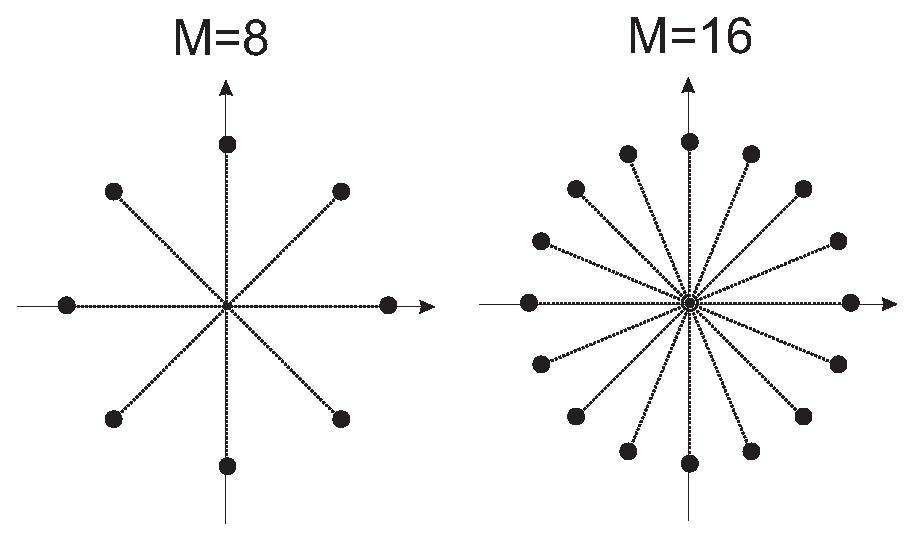
\includegraphics[width=0.5\textwidth]{../images/MPSK-signalSpaceDiagram.eps}}
  \caption{Signal space diagram for $M$-ary PSK for $M=8$ and $M=16$.}
  \label{F:MPSK-signalSpaceDiagram2}
\end{figure}
Essentially, we must find calculate the probability of symbol error
as 1 minus the area in the sector within $\pm \frac{\pi}{M}$ of the
correct angle $\phi_i$.  This is,
\begin{equation} \label{E:ExactMPSK-PE}
  P(\mbox{symbol error}) = 1 - \int_{r\in R_i} \frac{1}{2\pi \sigma^2} e^{-\frac{\| \mbr - \mbalpha_i \|^2}{2\sigma^2}}
\end{equation}
This integral is a double integral, and we don't generally have any
exact expression to use to express the result in general.


\subsection{Probability of Error in QPSK}
In QPSK, the probability of error is analytically tractable. Consider the QPSK constellation diagram, when Gray encoding is used. You have already calculated the decision regions for each symbol; now consider the decision region for the first bit. 

The decision is made using \emph{only} one dimension, of the received signal vector $\mbx$, specifically $x_1$. Similarly, the second bit decision is made using only $x_2$.  Also, the noise contribution to each element is independent.  The decisions are decoupled -- $x_2$ has no impact on the decision about bit one, and $x_1$ has no impact on the decision on bit two.  Since we know the bit error probability for each bit decision (it is the same as
bipolar PAM) we can see that the bit error probability is also
\begin{equation}\label{E:ExactQPSK_PBE}
  \PR{\mbox{error}} = \Q{ \sqrt{\frac{2\En_b }{N_0}}}
\end{equation}

This is an extraordinary result -- the bit rate will double in QPSK, but in theory, the bit error rate does not increase.  As we will show later, the bandwidth of QPSK is identical to that of BPSK.


\subsection{Neighbors}

For a particular symbol $i$ in a constellation, we define the concept of \emph{neighbors}.  These are the symbols $j$ which are necessary to draw the (Voronoi) decision region for symbol $i$.  That is, the perpendicular bisector of the line between $i$ and $j$ is one of the boundaries of the decision region for $i$.  We denote this set as $N(i)$.

The \emph{nearest neighbors} is the set of neighbors which are at the minimum distance $d_{i,j}$ for all $j$ in $N(i)$.  There may be several neighbors $j$ with exactly the same distance $d_{i,j}$, which is the reason the nearest neighbors is a set, but of course there is a minimum of one nearest neighbor of $i$.  We denote this set as $NN(i)$.

\Example{Listing Neighbor Symbols}

Consider the constellation in Figure \ref{F:ExampleVoronoiDiagramLabelledSolutions}.
\begin{enumerate}
\item What are the neighbors of 1, $N(1)$?
\item What are the nearest neighbors of 1, $NN(1)$?
\end{enumerate}

\Solution{ For (1), $N(1) = \{4,5,6,9,10\}$.  Note that 3 could be a neighbor, since we've only drawn the Voronoi boundaries within the $[0,1]^2$, and the line for $(10,3)$ may intersect with the line from $(1,10)$ far to the upper left of this figure.  For (2) just by looking at the plot, $NN(1)=\{4\}$.}

Generally, since we don't put symbols in random locations as was done for this plot, it is easier to define neighbors and nearest neighbors.

\begin{figure}[htbp]
  \centerline{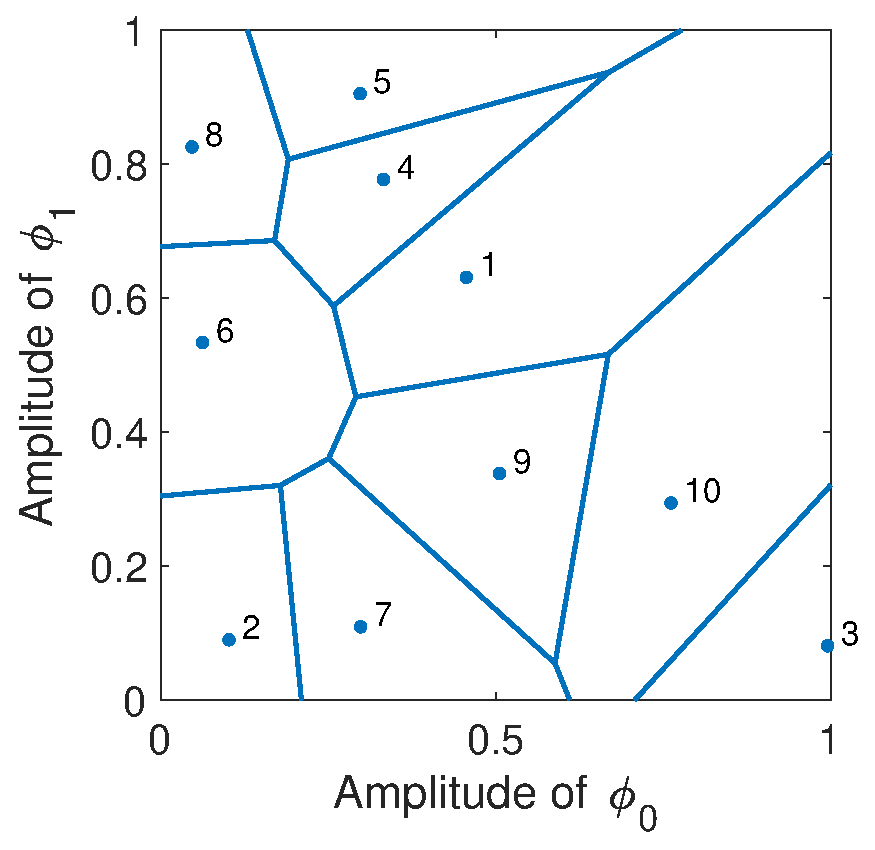
\includegraphics[width=0.8\textwidth]{../images/ExampleVoronoiDiagramLabelledSolutions.eps} }
  \caption{An example constellation diagram.  Find the neighbors and nearest neighbors of each symbol.  }
  \label{F:ExampleVoronoiDiagramLabelledSolutions}
\end{figure}


\subsection{Probability of $j|i$ Error}

What is the probability of deciding $H_j$ when $H_i$ is true?  When the space is divided into two, that is, there are no other symbols, this probability of being closer to $\mba_j$ than to $\mba_i$ can be computed with a 1-D integral of a Gaussian pdf.  Recall from probability that any linear combination of a multi-variate Gaussian vector is also Gaussian.  If we rotate the axes so that one is parallel to the line between $\mba_i$ and $\mba_j$ (which we call the \emph{new axis}, then this rotated vector is also multivariate Gaussian, and the distance along this new axis is Gaussian.  Further because the standard deviation is identical in every dimension, the standard deviation of the value on this new axis is also the same, $\sigma_W = \sqrt{N_0/2}$.  Let $y$ be the value along the new axis.

Consider the probability that, given $i$ was sent, that $y$ is closer to $j$ than to $i$ and thus we decide $H_j$.  Denote this event $E_{j|i}$.  Since $\mba_i$ and $\mba_j$ are $d_{i,j} = \| \mba_i - \mba_j\|$ apart, the threshold is halfway between, or  $d_{i,j}/2$ away from the $\mba_i$.  The probability is
\begin{equation} \label{E:RicePairwiseErrorPrep}
  \PR{E_{j|i}} = \Q{ 
  \frac{d_{i,j}/2}{\sqrt{N_0/2}}
  }
  = 
  \Q{
  \sqrt{\frac{d_{i,j}^2}{4}}\sqrt{\frac{2}{N_0}}
  }
  = 
  \Q{ 
  \sqrt{\frac{d_{i,j}^2}{2N_0}}
  }
\end{equation}

We often want the  \emph{pairwise probability of error} in terms of $\Ebno$ or $\En_s/N_0$.  To make this more explicit, I am also showing the first step in how to get this expression:
\begin{equation} \label{E:RicePairwiseError_a}
  \PR{E_{j|i}} = \Q{\sqrt{\frac{d^2_{i,j}}{2N_0}}}
  = \Q{\sqrt{\frac{d^2_{i,j}}{2\En_s}\frac{\En_s}{N_0}}}
  = \Q{\sqrt{\frac{d^2_{i,j}}{2\En_b}\frac{\En_b}{N_0}}}
\end{equation}
If we use a constant $A$ when describing the signal space vectors (as we usually do), then, since $\En_s$ will be proportional to $A^2$ and $d^2_{m,n}$ will be proportional to $A^2$, the factors $A$ will cancel out of the expression.

A more detailed proof of (\ref{E:RicePairwiseError_a}) is detailed in Section 6.2 of the Rice book.





\subsection{Union Bound}

From 5510 or an equivalent class (or a Venn diagram) you may recall
the probability formula, that for two events $E$ and $F$ that
\[
  \PR{E \cup F} = \PR{E} + \PR{F} - \PR{E \cap F}
\]
You can prove this from the three axioms of probability. (This holds
for \emph{any} events $E$ and $F$!) Then, using the above formula,
and the first axiom of probability, we have that
\begin{equation} \label{E:UnionBound2}
  \PR{E \cup F} \le \PR{E} + \PR{F}.
\end{equation}
Furthermore, from (\ref{E:UnionBound2}) it is straightforward to
show that for \emph{any} list of sets $E_1, E_2, \ldots E_n$ we have
that
\begin{equation} \label{E:UnionBound}
  \PR{ \bigcup_{i=1}^n E_i } \le \sum_{i=1}^n \PR{E_i}
\end{equation}
This is called the \emph{union bound}, and it is very useful across
communications.  If you know one inequality, know this one.  It is
useful when the overlaps $E_i \cap E_j$ are small but difficult to
calculate.  

\begin{figure}[htbp]
  \centerline{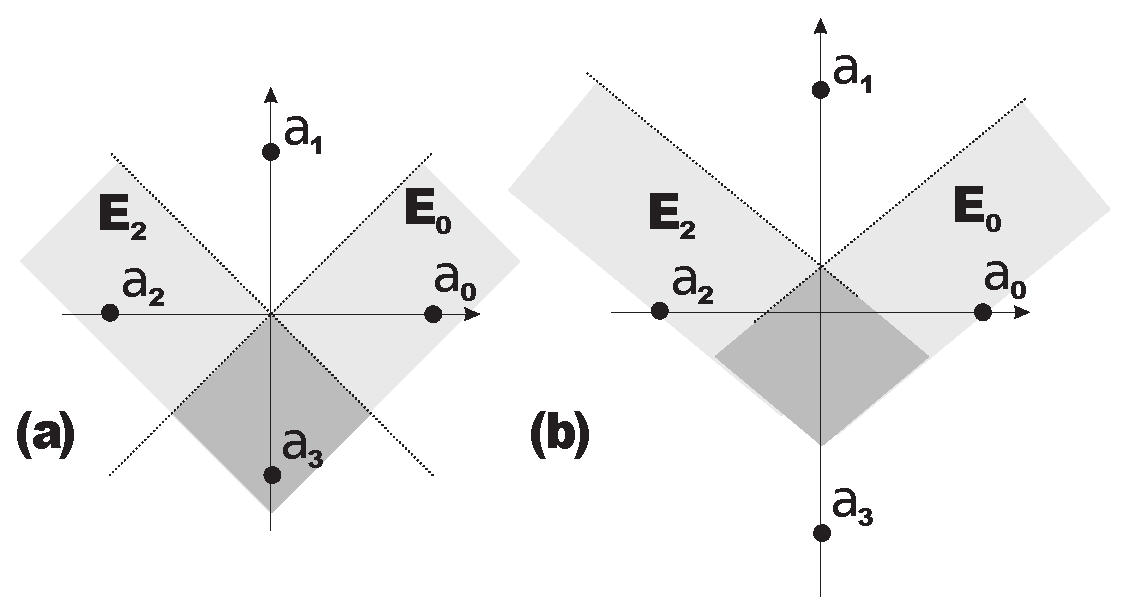
\includegraphics[width=0.7\textwidth]{../images/UnionBoundEg2.eps} }
  \caption{Union bound examples. (a) is QPSK with symbols of equal energy
    $\sqrt{\En_s}$.  In (b) $\mba_1 = -\mba_3 = [0, \sqrt{3\En_s/2}]^T$
    and $\mba_2 = -\mba_0 = [\sqrt{\En_s/2},0]^T$.  }
  \label{F:UnionBoundEg}
\end{figure}

\Example{QPSK}  First, let's study the union bound for QPSK, as
shown in Figure \ref{F:UnionBoundEg}(a).  Assume $s_1(t)$ is sent.
We know that from our previous lecture on square QAM:
\begin{equation} 
  P(\mbox{bit error}) \approx \frac{4(\sqrt{M}-1)}{\sqrt{M} \log_2 M} \Q{\sqrt{\frac{3 \log_2 M}{M-1} \frac{\En_b}{N_0}}}.
\end{equation}
For $M=4$, this result uses $\sqrt{M}=2$ and $\log_2 M = 2$, thus:
\begin{equation} \label{E:PrSymbolErrorMPAM_review}
  P(\mbox{bit error}) \approx \frac{4}{2 (2)} \Q{\sqrt{\frac{3 (2)}{3} \frac{\En_b}{N_0}}}.
\end{equation}
Or
\[
  \PR{\mbox{bit error}} = \Q{\sqrt{\frac{2 \En_b}{ N_0}}}
\]
The probability of symbol error is one minus the probability that there were no error in either bit,
\begin{equation}\label{E:UnionBoundEg1a}
  \PR{\mbox{symbol error}} = 1-\left(1-\Q{\sqrt{\frac{2 \En_b}{ N_0}}}\right)^2
\end{equation}
We can also write this as:
\begin{equation}\label{E:UnionBoundEg1b}
  \PR{\mbox{symbol error}} = 2\Q{\sqrt{\frac{2 \En_b}{ N_0}}} - \left[ 2\Q{\sqrt{\frac{2 \En_b}{ N_0}}}\right]^2
\end{equation}

In contrast, let's calculate the union bound on the probability of
error. There are two neighbors of each node $i$.  Consider for example node $i=1$.  We can write
\[
  \PR{\mbox{symbol error} | H_1} = \PR{E_2 \cup E_0}
\]
We ignored $E_3$ because it overlaps completely with $E_2 \cup E_0$.
That is, $E_2 \cup E_0 \cup E_3 = E_2 \cup E_0$.

Then, we use the union bound.
\[
  \PR{\mbox{symbol error} | H_1} \le  \PR{E_2} + \PR{E_0}
\]
These two probabilities are just the probability of error for a
binary modulation, and both are identical, so
\[
  \PR{\mbox{symbol error} | H_1} \le  2 \Q{\sqrt{\frac{2 \En_b}{ N_0}}}
\]

The overall probability of error is the average of $\PR{\mbox{symbol error} | H_i}$ for $i=0,1,2,3$; however these will all be identical due to the symmetry of QPSK.  Thus $\PR{\mbox{symbol error} } = \PR{\mbox{symbol error} | H_1}$.


What is missing / What is the difference in this expression compared
to (\ref{E:UnionBoundEg1b})?

See Figure \ref{F:PERPlotUnionBound} to see the union bound
probability of error plot, compared to the exact expression.  Only
at very low $E_b/N_0$ is there any noticeable difference!

\begin{figure}[htbp]
  \centerline{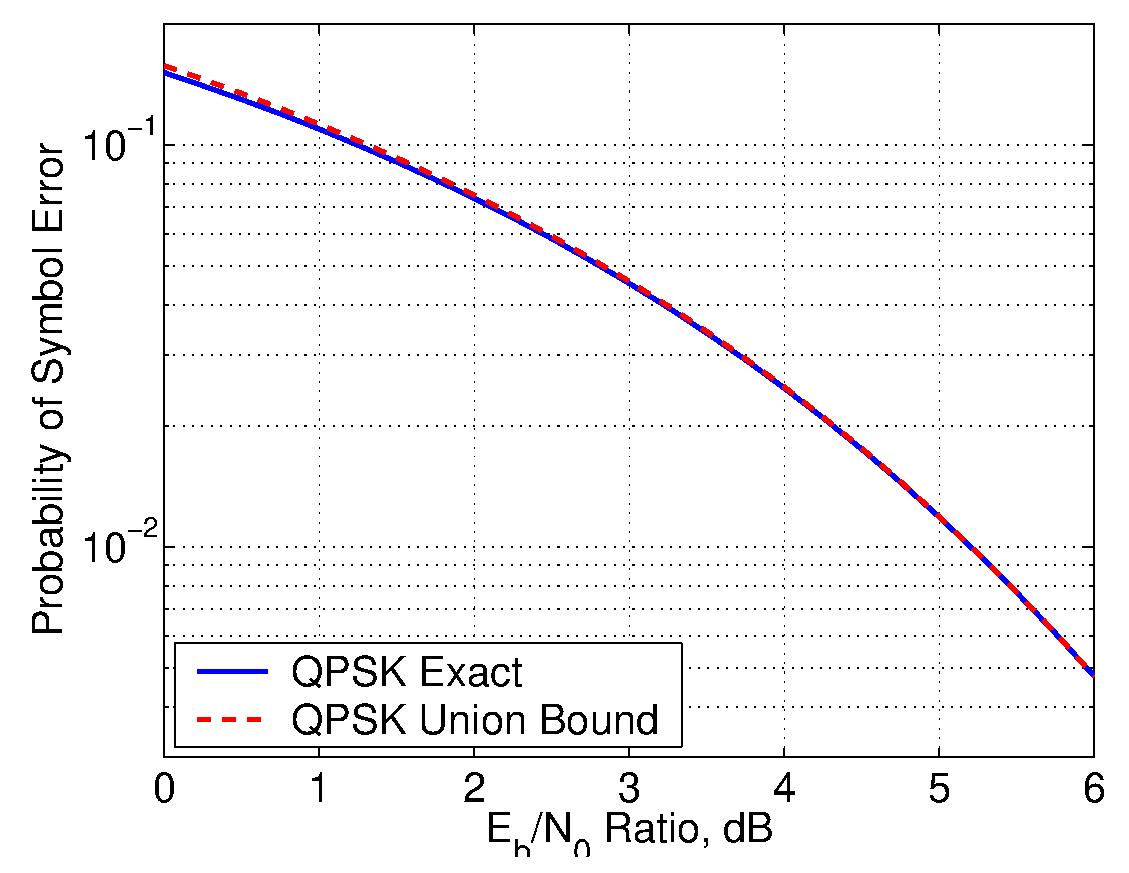
\includegraphics[width=0.75\textwidth]{../images/plotProbBitErrPSK_UnionBound.eps} }
  \caption{For QPSK, the exact probability of symbol error expression vs.\ the union bound.  }
  \label{F:PERPlotUnionBound}
\end{figure}


\subsection{General Application of Union Bound}

In this class, our events are typically error events.  Let $E_{j|i}$  represent the event that we decide $H_j$, when a different
symbol $i$ was actually sent.  In this case,  the union bound can be used to find the overall error given that $i$ was sent:
\begin{equation} \label{E:UnionBound_5}
  \PR{ \mbox{symbol error} | H_i } \le \sum_{j\in N(i)} \PR{E_{j|i}}
\end{equation}
These events $E_{j|i}$ for all $j\in N(i)$ cover all of the area outside of the decision region for $i$.  That is, by combining their $\PR{E_{j|i}}$, we are greater than or equal to the probability of error given symbol $i$ was sent.  

The overall probability of error, averaged over all $i$ that could be sent, is 
\begin{equation} \label{E:UnionBoundMid}
  \PR{ \mbox{symbol error} } \le \frac{1}{M} \sum_{i=0}^{M-1} \sum_{j\in N(i)} \PR{E_{j|i}} 
\end{equation}
Using the formula from (\ref{E:RicePairwiseError_a}),
\begin{equation} \label{E:UnionBound_applied}
  \PR{ \mbox{symbol error} } \le \frac{1}{M} \sum_{i=0}^{M-1} \sum_{j\in N(i)}  \Q{\sqrt{\frac{d^2_{i,j}}{2N_0}}}
\end{equation}

The union bound gives a conservative estimate.  This can be useful
for quick initial study of a modulation type.

\subsubsection{Rice book formula}
This is the formula for the Union bound given in Rice book:
\begin{eqnarray} \label{E:RiceUnionBound}
  \PR{\mbox{symbol error}} &\le & \frac{1}{M} \sum_{m=0}^{M-1} \sum_{n=0 \atop n\neq m}^{M-1} \PR{\mbox{decide } H_n | H_m}
 \nn
\end{eqnarray}
Note the $\le$ sign.  This means the actual $\PR{\mbox{symbol error}}$ will be \textit{at most} this value.  It is probably less than this value.  This is a general formula and \textit{is not necessarily the best} upper bound.  What do we mean?  If I draw any function that is always above the actual $\PR{\mbox{symbol error}}$ formula, I have drawn an upper bound.  But I could draw lots of functions that are upper bounds, some higher than others.

In particular, for some of the error events, decide $H_n | H_m$ may be redundant, and do not need to be included.  We have talked about the concept of ``neighboring'' symbols and ``nearest neighboring'' symbols to symbol $i$, which we call respectively, $N(i)$ and $NN(i)$.  The $N(i)$ are the ones that are necessary to include in the union bound.

Note that the Rice book uses $E_{avg}$ where I use $\En_s$ to denote
average symbol energy.  The Rice book uses $E_b$ where I use $\En_b$
to denote average bit energy. 



\Example{4-QAM with two amplitude levels}  This is shown (poorly) in
Figure \ref{F:UnionBoundEg}(b).  The amplitudes of the top and
bottom symbols are $\sqrt{3}$ times the amplitude of the symbols on
the right and left.  (They are positioned to keep the distance
between points in the signal space equal to $\sqrt{2\En_s/N_0}$.)  I
am calling this ``2-amplitude 4-QAM'' (I made it up).

What is the union bound on the probability of symbol error, given
$H_1$? 

\Solution{ Given symbol 1, the probability is the same as
above. Defining $E_2$ and $E_0$ as above, these two distances
between symbol $\mba_1$ and $\mba_2$ or $\mba_0$ are the same:
$\sqrt{2\En_s/N_0}$. Thus the formula for the union bound is the
same.}

What is the union bound on the probability of symbol error, given
$H_2$? \Solution{Now, it is
\[
  \PR{\mbox{symbol error} | H_2} \le  3 \Q{\sqrt{\frac{2 \En_b}{ N_0}}}
\]
}

So, overall, the union bound on probability of symbol error is
\[
  \PR{\mbox{symbol error} } \le  \frac{3\cdot 2 + 2\cdot 2}{4} \Q{\sqrt{\frac{2 \En_b}{ N_0}}} = 2.5 \Q{\sqrt{\frac{2 \En_b}{ N_0}}}.
\]

How about average energy? For QPSK, the symbol energies are all
equal.  Thus $\En_{av} = \En_s$.  For the two-amplitude 4-QAM
modulation,
\[
  \En_{av} = \En_s \frac{2(0.5) + 2(1.5)}{4} = \En_s
\]
Thus there is no advantage to the two-amplitude QAM modulation in
terms of average energy.





\subsection{Nearest-Neighbor Approximate Probability of Error}

As it turns out, the probability of error is often well approximated
by the terms in the Union Bound with the smallest
$d_{i,j}$.  This is because higher $d_{i,j}$ means a higher argument
in the Q-function, which in turn means a lower value of the
Q-function.  A little extra distance means a much lower value of the
Q-function.  So approximately,
\begin{eqnarray} \label{E:NearestNeighborApproximatePError}
  \PR{\mbox{symbol error}}  &\approx & \frac{N_{min}}{M}  \Q{\sqrt{\frac{d^2_{min}}{2N_0}}} \nn
\end{eqnarray}
where
\[
  d_{min} = \min_{j\neq i} d_{i,j}, \quad m,n \in \{0, \ldots, M-1\}
\]
and $N_{min}$ is the number of \emph{ordered pairs} of symbols which are separated by distance $d_{min}$.  Be sure to double count each pair, otherwise this formula won't work!

\Example{2-Amplitude 4-QAM}
What is the nearest neighbor approximation for 2-Amplitude 4-QAM?

\Solution{
The minimum distance $d_{min} = 2A  = \sqrt{2\En_s}$.  Starting from symbol 0, I count 3, 2, 3, and 2 such distances.  This is a total of $N_{min} = 10$.  Thus
\[
\PR{\mbox{symbol error}}  \approx  \frac{10}{4}  \Q{\sqrt{\frac{2\En_b}{N_0}}} \nn
\]
The same as the Union Bound.
}

 
\StartOf{Lecture 14}

\Today{Probability of Error (1) QAM / PSK  examples, (2) FSK, (3) Differential PSK}


\subsection{QAM/PSK Probability of Error Examples}
\Example{Probability of Error in $M$-PSK}

Find the probability of error in $M$-ary PSK using the nearest neighbor approximation.  Is this the same as the union bound?

\vspace{0.1in}
\Solution{
Here the distance between two neighboring symbols can be calculated by seeing the origin and the two symbol points as forming an isosceles triangle with top angle $2\pi/M$, and equal sides having length $A$.  Thus the length of the base is $d_{min} = 2A\sin \frac{2\pi}{2M}$.  The squared distance is
\[
d_{min}^2 = 4A^2 \sin^2 (\pi/M)
\]

The average energy per symbol is simply $A^2$ because all of the symbol points are $A$ from the origin.  Thus the average energy per bit is $\En_b = A^2 / \log_2 M$.  Thus $A^2 = \En_b \log_2 M$.  So:
\[
d_{min}^2 = 4\En_b (\log_2 M ) \sin^2 (\pi/M)
\]

Using the expression for the nearest neighbor approximation:
\begin{eqnarray} \label{E:MPSK_Perror_approx}
  \PR{\mbox{symbol error}} &\approx & \frac{N_{min}}{M}  \Q{\sqrt{\frac{d^2_{min}}{2N_0}}} \nnn
  &\approx& \frac{2M}{M} \Q{\sqrt{4 (\log_2 M)\sin^2 ( \pi/M ) \frac{\En_b }{2N_0}}} \nnn
    &\approx& 2 \Q{\sqrt{2 (\log_2 M)\sin^2 ( \pi/M ) \frac{\En_b }{N_0}}} \nn
\end{eqnarray}

This is the same as the union bound because each symbol only has two neighbors (symbols that contribute to the decision boundary). 
}

The Rice book, Section 6.2, page 319-321, derives an approximate formula for the probability of error in $M$-PSK for $M>4$.  (Recall QPSK has an exact solution.)  For $M>4$, the book shows how to use a polar transformation and approximate the probability of error integral.  The solution is exactly the same, in the end, as the nearest neighbor approximation / union bound expression in (\ref{E:MPSK_Perror_approx}).  




\Example{Additional QAM / PSK Constellations}

Solve for the probability of symbol error in the completely made up signal space diagrams in
Figure \ref{F:exampleQAM-PSK-diagrams}.  You should calculate:
\begin{itemize}
  \item An exact expression if one should happen to be available,
  \item The union bound,
  \item The nearest-neighbor approximation.
\end{itemize}
Solve for the probability of symbol error first, and next the probability of
bit error.  Figure \ref{F:exampleQAM-PSK-diagrams} is in terms of amplitude $A$, but all
probability of error expressions should be written in terms of
$\En_b/N_0$.

\begin{figure}[htbp]
  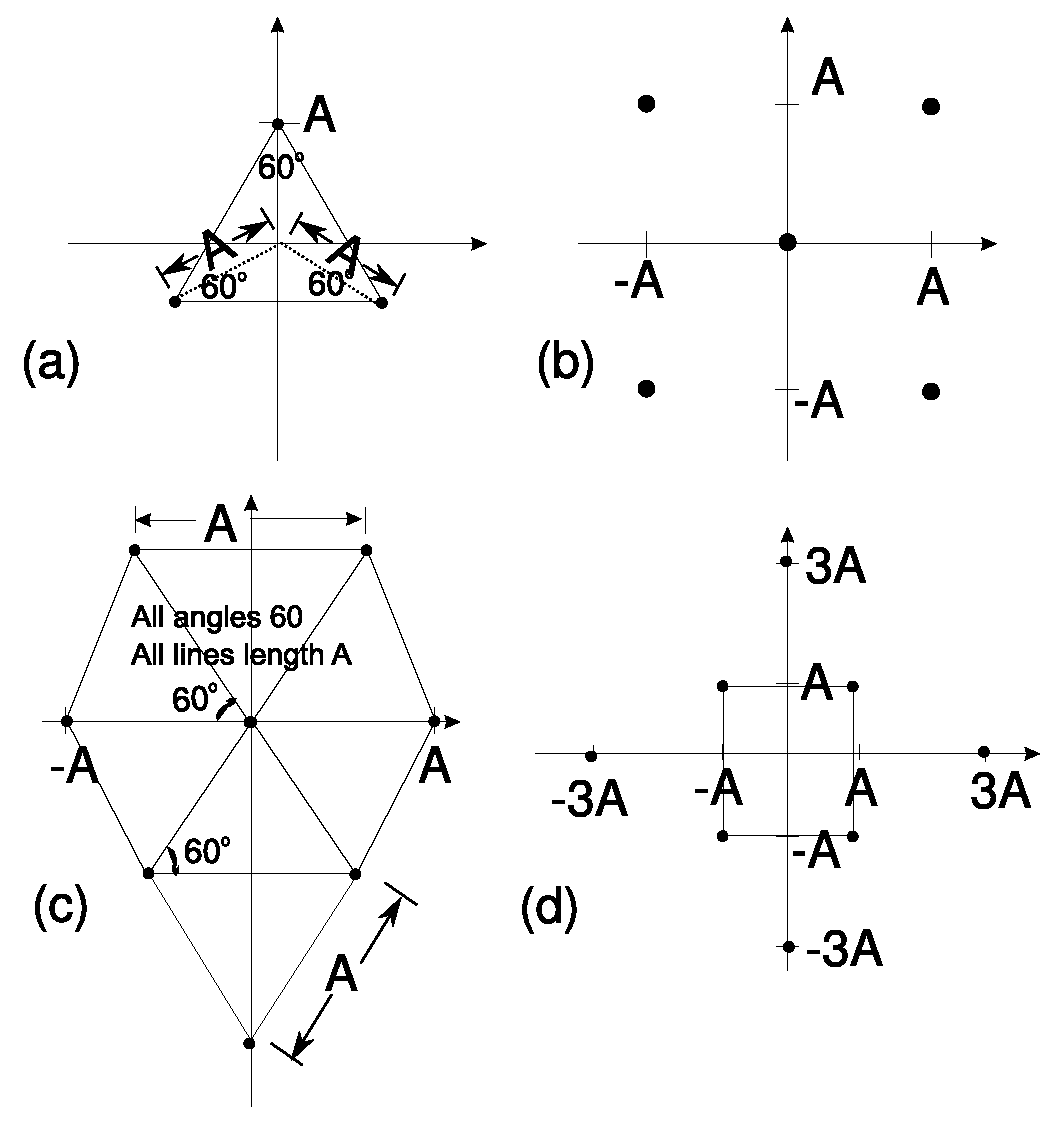
\includegraphics[width=0.9\textwidth]{../images/EgQAM_v2.eps}
  \caption{Constellation diagram for some example (made up) modulations.
  \label{F:exampleQAM-PSK-diagrams}}
\end{figure}
\begin{figure}[htbp]
  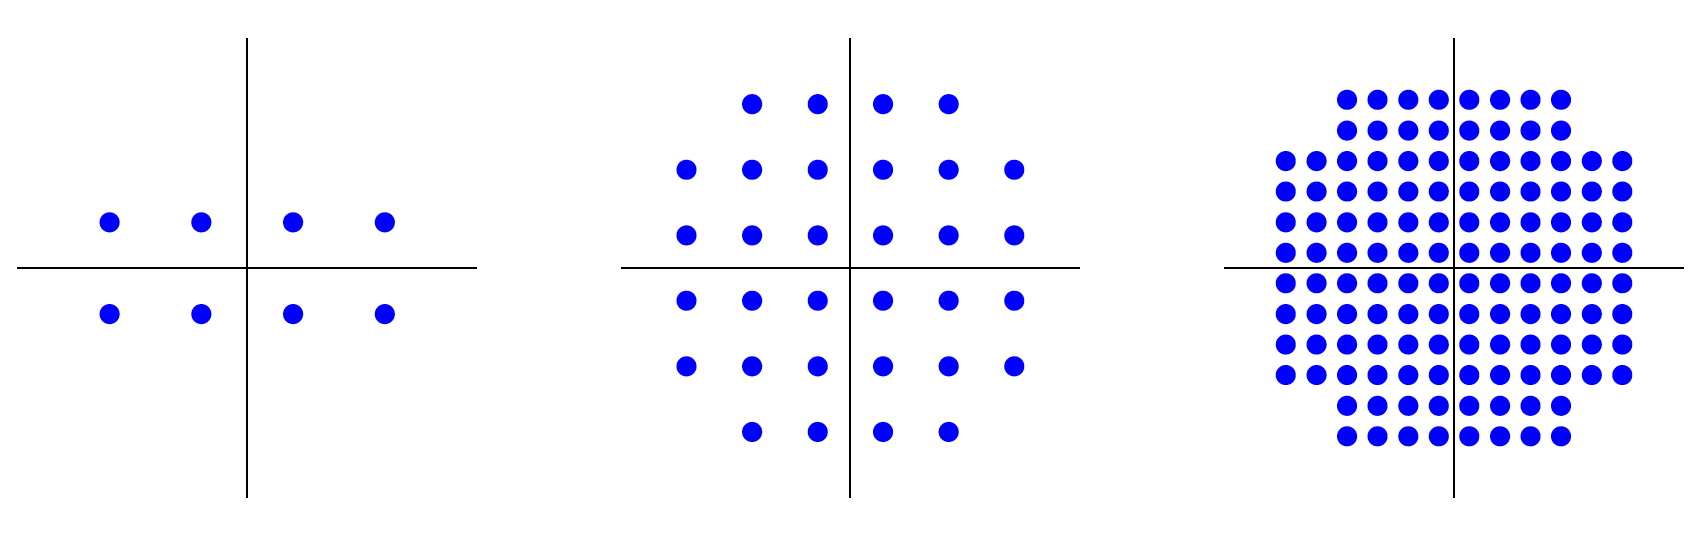
\includegraphics[width=1.0\textwidth]{../images/cross_mqam_8_32_64.png}
  \caption{Constellation diagrams for Cross M-QAM for (left) $M=8$, (center) $M=32$, and (right) $M=64$, from Rice Figure 5.3.4.
  \label{F:exampleCrossQAM}}
\end{figure}

\Example{2 by 4 grid QAM}
Solve for the probability of symbol error in the signal space diagrams in
Rice Figure 5.3.4 (a), copied in these notes as Figure \ref{F:exampleCrossQAM} (left).  You should calculate:
\begin{itemize}
  \item An exact expression,
  \item The union bound,
  \item The nearest-neighbor approximation.
\end{itemize}

\Solution{(a) An exact expression is possible because the decision is separable.  That is, the $x_0$ will decide two of the three bits, while $x_1$ will decide the third bit.  Assume that nearest neighbors are separated by 2A.  For the third bit, the probability of error is that of bipolar PAM, that is, $\Q{\sqrt{\frac{2 A^2}{N_0}}}$.  For the first two bits, the probability of bit error is approximately (assuming Gray coding),
\[
\frac{1}{\log_2 M} \frac{2(M-1)}{M} \Q{\sqrt{\frac{2 A^2}{N_0}}} =  \frac{3}{4} \Q{\sqrt{\frac{2 A^2}{N_0}}}  
\]
The overall average probability of error will be a weighted average of these two -- 2/3 times the probability of bit error in the first two bits and 1/3 times the probability of bit error in the third bit,
\[
 \PR{\mbox{bit error}} \approx \left[ \frac{2}{3}\frac{3}{4}+ \frac{1}{3}\right] \Q{\sqrt{\frac{2 A^2}{N_0}}} = \frac{5}{6}\Q{\sqrt{\frac{2 A^2}{N_0}}}
\]
The average bit energy is 
\begin{eqnarray}
 \En_b &=& \frac{1}{\log_2 8} \En_s\\
 &=& \frac{1}{\log_2 8} \frac{1}{8}\left[ 4(2A^2) + 4*(A^2 + 9A^2)\right] = 2A^2
\end{eqnarray}
Thus 
\[
 \PR{\mbox{bit error}} = \frac{5}{6}\Q{\sqrt{\frac{\En_b}{ N_0}}}
\]

The union bound for (a) and the nearest neighbor approximation are the same.  All nearest neighbors are separated by distance 2A.  Four nodes have two neighbors, and four nodes have three neighbors.  So $N_{min} = 20$, and $d_{min}=2A$. 
So,
\begin{eqnarray} 
  \PR{\mbox{symbol error}}  &\le & \frac{20}{8} \Q{\sqrt{\frac{4A^2}{2N_0}}} = 2.5 \Q{\sqrt{\frac{\En_b}{N_0}}} \nonumber
\end{eqnarray}
Note that this results in an approximate bit error rate of $\frac{5}{6} \Q{\sqrt{\frac{\En_b}{N_0}}}$, the same expression as above.}

\Example{Cross $M=32$ QAM}
Solve for the probability of symbol error in the signal space diagrams in
Rice Figure 5.3.4 (b), copied to these notes as Figure \ref{F:exampleCrossQAM} (center).  You should calculate:
\begin{itemize}
  \item The union bound, and
  \item The nearest-neighbor approximation.
\end{itemize}

\Solution{
The union bound requires us to count neighbors. Assume all nearest neighbors are separated by distance 2A.  
\begin{enumerate}
 \item Sixteen nodes (the center 4x4 grid) have four neighbors at distance $2A$,
 \item Eight nodes have three neighbors at distance $2A$,
 \item Eight nodes have two neighbors at distance $2A$ and one neighbor at distance $2\sqrt{2}A$.  
\end{enumerate}
Also, the average symbol energy is $\frac{1}{32}$ times twice the sum of the squared x-coordinates because of the symmetry of the constellation.
\[
 \En_s = \frac{2(12A^2 + 12(9A^2) + 8(25A^2))}{32} = 20A^2
\]
Since $\log_2 M = 5$, we have $\En_b = \frac{\En_s}{5}  =  4A^2$.
\begin{eqnarray} 
  \PR{\mbox{symbol error}}  &\le & \frac{1}{32} \left\{ (16(4)+8(3)+8(2)) \Q{\sqrt{\frac{4A^2}{2N_0}}} + 8\Q{\sqrt{\frac{8A^2}{2N_0}}} \right\} \nnn
  &\le& \frac{13}{4}\Q{\sqrt{\frac{\En_b}{2 N_0}}} + \frac{1}{4}\Q{\sqrt{\frac{\En_b}{N_0}}}
\end{eqnarray}
The nearest neighbor approximation would simply remove the second term and replace the $\le$ with an $\approx$.
}





\section{FSK Probability of Error}

\subsection{Probability of Error for Coherent Binary FSK}

First, let's look at coherent detection of binary FSK.
\begin{enumerate}
 \item What is the detection threshold line separating the two decision
regions?
 \item What is the distance between points in the Binary FSK signal space?
\end{enumerate}
What is the probability of error for coherent binary FSK?  It
is the same as bipolar PAM, but the symbols are spaced differently (more closely) as a function of $\En_b$.  We had that
\[
\PR{\mbox{error}}_{2-ary} = \Q{\sqrt{\frac{d_{0,1}^2}{2N_0}}}
\]
Now, the spacing between symbols has reduced by a factor of $\sqrt{2}/2$ compared to bipolar PAM, to $d_{0,1} = \sqrt{2\En_b}$.  So
\[
\PR{\mbox{error}}_{2-Co-FSK} = \Q{\sqrt{\frac{\En_b}{N_0}}}
\]
For the same probability of bit error, binary FSK is about 1.5 dB better than OOK (requires 1.5 dB less energy per bit), but 1.5 dB worse than bipolar PAM (requires 1.5 dB more energy per bit).


\begin{figure}[htbp]
  (a) 


\tikzset{every picture/.style={line width=0.75pt}} %set default line width to 0.75pt        

\begin{tikzpicture}[x=0.75pt,y=0.75pt,yscale=-1,xscale=1]
%uncomment if require: \path (0,378); %set diagram left start at 0, and has height of 378

%Straight Lines [id:da015204313020472648] 
\draw    (100,127) -- (120,127) ;
%Straight Lines [id:da3807433535655065] 
\draw    (120,174) -- (120,82) ;
%Straight Lines [id:da13452699900895748] 
\draw    (120,82) -- (146,82) ;
\draw [shift={(149,82)}, rotate = 180] [fill={rgb, 255:red, 0; green, 0; blue, 0 }  ][line width=0.08]  [draw opacity=0] (8.93,-4.29) -- (0,0) -- (8.93,4.29) -- cycle    ;
%Shape: Rectangle [id:dp6831503614766208] 
\draw   (222,63) -- (311,63) -- (311,101) -- (222,101) -- cycle ;
%Shape: Circle [id:dp5132093237924611] 
\draw   (149,82) .. controls (149,74.82) and (154.82,69) .. (162,69) .. controls (169.18,69) and (175,74.82) .. (175,82) .. controls (175,89.18) and (169.18,95) .. (162,95) .. controls (154.82,95) and (149,89.18) .. (149,82) -- cycle ;
%Straight Lines [id:da25287195023205933] 
\draw    (155,75) -- (169,90) ;
%Straight Lines [id:da5242592168562576] 
\draw    (169,75) -- (154,90) ;
%Straight Lines [id:da23051729614765581] 
\draw    (162.09,66) -- (162.5,53) ;
\draw [shift={(162,69)}, rotate = 271.79] [fill={rgb, 255:red, 0; green, 0; blue, 0 }  ][line width=0.08]  [draw opacity=0] (8.93,-4.29) -- (0,0) -- (8.93,4.29) -- cycle    ;
%Straight Lines [id:da2971482914437682] 
\draw    (175,82) -- (220,82) ;
\draw [shift={(223,82)}, rotate = 180] [fill={rgb, 255:red, 0; green, 0; blue, 0 }  ][line width=0.08]  [draw opacity=0] (8.93,-4.29) -- (0,0) -- (8.93,4.29) -- cycle    ;
%Straight Lines [id:da24289517343868772] 
\draw    (311,82) -- (359,82) -- (380,66) ;
%Straight Lines [id:da03913348203652922] 
\draw    (376,82) -- (452.24,82) ;
\draw [shift={(455.24,82)}, rotate = 180] [fill={rgb, 255:red, 0; green, 0; blue, 0 }  ][line width=0.08]  [draw opacity=0] (8.93,-4.29) -- (0,0) -- (8.93,4.29) -- cycle    ;
%Curve Lines [id:da6656366911860763] 
\draw    (354.83,73.33) .. controls (364.08,72.41) and (363.64,74.62) .. (369.85,83.66) ;
\draw [shift={(371.5,86)}, rotate = 233.97] [fill={rgb, 255:red, 0; green, 0; blue, 0 }  ][line width=0.08]  [draw opacity=0] (8.93,-4.29) -- (0,0) -- (8.93,4.29) -- cycle    ;
%Shape: Rectangle [id:dp38931328167896195] 
\draw   (455.24,51) -- (508.5,51) -- (508.5,201) -- (455.24,201) -- cycle ;
%Straight Lines [id:da5073149386864682] 
\draw    (508,126) -- (534,126) ;
\draw [shift={(537,126)}, rotate = 180] [fill={rgb, 255:red, 0; green, 0; blue, 0 }  ][line width=0.08]  [draw opacity=0] (8.93,-4.29) -- (0,0) -- (8.93,4.29) -- cycle    ;
%Straight Lines [id:da0935600260327849] 
\draw    (120,174) -- (146,174) ;
\draw [shift={(149,174)}, rotate = 180] [fill={rgb, 255:red, 0; green, 0; blue, 0 }  ][line width=0.08]  [draw opacity=0] (8.93,-4.29) -- (0,0) -- (8.93,4.29) -- cycle    ;
%Shape: Rectangle [id:dp5397600807528802] 
\draw   (222,155) -- (311,155) -- (311,193) -- (222,193) -- cycle ;
%Shape: Circle [id:dp6340079603545306] 
\draw   (149,174) .. controls (149,166.82) and (154.82,161) .. (162,161) .. controls (169.18,161) and (175,166.82) .. (175,174) .. controls (175,181.18) and (169.18,187) .. (162,187) .. controls (154.82,187) and (149,181.18) .. (149,174) -- cycle ;
%Straight Lines [id:da054936665320719724] 
\draw    (155,167) -- (169,182) ;
%Straight Lines [id:da14446384117365363] 
\draw    (169,167) -- (154,182) ;
%Straight Lines [id:da06806069680494597] 
\draw    (162.09,158) -- (162.5,145) ;
\draw [shift={(162,161)}, rotate = 271.79] [fill={rgb, 255:red, 0; green, 0; blue, 0 }  ][line width=0.08]  [draw opacity=0] (8.93,-4.29) -- (0,0) -- (8.93,4.29) -- cycle    ;
%Straight Lines [id:da13918324188613052] 
\draw    (175,174) -- (220,174) ;
\draw [shift={(223,174)}, rotate = 180] [fill={rgb, 255:red, 0; green, 0; blue, 0 }  ][line width=0.08]  [draw opacity=0] (8.93,-4.29) -- (0,0) -- (8.93,4.29) -- cycle    ;
%Straight Lines [id:da7726545291977289] 
\draw    (311,174) -- (359,174) -- (380,158) ;
%Straight Lines [id:da5999576449313313] 
\draw    (376,174) -- (452.24,174) ;
\draw [shift={(455.24,174)}, rotate = 180] [fill={rgb, 255:red, 0; green, 0; blue, 0 }  ][line width=0.08]  [draw opacity=0] (8.93,-4.29) -- (0,0) -- (8.93,4.29) -- cycle    ;
%Curve Lines [id:da38919606803399187] 
\draw    (354.83,165.33) .. controls (364.08,164.41) and (363.64,166.62) .. (369.85,175.66) ;
\draw [shift={(371.5,178)}, rotate = 233.97] [fill={rgb, 255:red, 0; green, 0; blue, 0 }  ][line width=0.08]  [draw opacity=0] (8.93,-4.29) -- (0,0) -- (8.93,4.29) -- cycle    ;

% Text Node
\draw (189,38) node    {$\sqrt{2}\cos( \omega _{0} t+\phi _{0})$};
% Text Node
\draw (266.5,82) node   [align=left] {matched\\filter p(-t)};
% Text Node
\draw (367,53) node    {$t=kT_{s}$};
% Text Node
\draw (429,64) node    {$r_{0}( kT_{s})$};
% Text Node
\draw (484.87,123.5) node  [rotate=-269.97] [align=left] {decision};
% Text Node
\draw (549,122) node    {$\hat{\mathbf{a}}$};
% Text Node
\draw (77,127) node    {$r( t)$};
% Text Node
\draw (189,130) node    {$\sqrt{2}\cos( \omega _{1} t+\phi _{1})$};
% Text Node
\draw (266.5,174) node   [align=left] {matched\\filter p(-t)};
% Text Node
\draw (367,145) node    {$t=kT_{s}$};
% Text Node
\draw (429,156) node    {$r_{1}( kT_{s})$};


\end{tikzpicture}
  
  (b) 


\tikzset{every picture/.style={line width=0.75pt}} %set default line width to 0.75pt        

\begin{tikzpicture}[x=0.75pt,y=0.75pt,yscale=-1,xscale=1]
%uncomment if require: \path (0,378); %set diagram left start at 0, and has height of 378

%Straight Lines [id:da015204313020472648] 
\draw    (100,203) -- (120,203) ;
%Straight Lines [id:da3807433535655065] 
\draw    (120,148) -- (120,82) ;
%Straight Lines [id:da13452699900895748] 
\draw    (120,82) -- (146,82) ;
\draw [shift={(149,82)}, rotate = 180] [fill={rgb, 255:red, 0; green, 0; blue, 0 }  ][line width=0.08]  [draw opacity=0] (8.93,-4.29) -- (0,0) -- (8.93,4.29) -- cycle    ;
%Shape: Rectangle [id:dp6831503614766208] 
\draw   (222,63) -- (311,63) -- (311,101) -- (222,101) -- cycle ;
%Shape: Circle [id:dp5132093237924611] 
\draw   (149,82) .. controls (149,74.82) and (154.82,69) .. (162,69) .. controls (169.18,69) and (175,74.82) .. (175,82) .. controls (175,89.18) and (169.18,95) .. (162,95) .. controls (154.82,95) and (149,89.18) .. (149,82) -- cycle ;
%Straight Lines [id:da25287195023205933] 
\draw    (155,75) -- (169,90) ;
%Straight Lines [id:da5242592168562576] 
\draw    (169,75) -- (154,90) ;
%Straight Lines [id:da23051729614765581] 
\draw    (162.09,66) -- (162.5,53) ;
\draw [shift={(162,69)}, rotate = 271.79] [fill={rgb, 255:red, 0; green, 0; blue, 0 }  ][line width=0.08]  [draw opacity=0] (8.93,-4.29) -- (0,0) -- (8.93,4.29) -- cycle    ;
%Straight Lines [id:da2971482914437682] 
\draw    (175,82) -- (220,82) ;
\draw [shift={(223,82)}, rotate = 180] [fill={rgb, 255:red, 0; green, 0; blue, 0 }  ][line width=0.08]  [draw opacity=0] (8.93,-4.29) -- (0,0) -- (8.93,4.29) -- cycle    ;
%Straight Lines [id:da24289517343868772] 
\draw    (311,82) -- (359,82) -- (380,66) ;
%Straight Lines [id:da03913348203652922] 
\draw    (376,82) -- (421.86,106.58) ;
\draw [shift={(424.5,108)}, rotate = 208.19] [fill={rgb, 255:red, 0; green, 0; blue, 0 }  ][line width=0.08]  [draw opacity=0] (8.93,-4.29) -- (0,0) -- (8.93,4.29) -- cycle    ;
%Curve Lines [id:da6656366911860763] 
\draw    (354.83,73.33) .. controls (364.08,72.41) and (363.64,74.62) .. (369.85,83.66) ;
\draw [shift={(371.5,86)}, rotate = 233.97] [fill={rgb, 255:red, 0; green, 0; blue, 0 }  ][line width=0.08]  [draw opacity=0] (8.93,-4.29) -- (0,0) -- (8.93,4.29) -- cycle    ;
%Straight Lines [id:da8443900724542854] 
\draw    (120,166) -- (120,100) ;
%Straight Lines [id:da5599679464635203] 
\draw    (120,165) -- (146,165) ;
\draw [shift={(149,165)}, rotate = 180] [fill={rgb, 255:red, 0; green, 0; blue, 0 }  ][line width=0.08]  [draw opacity=0] (8.93,-4.29) -- (0,0) -- (8.93,4.29) -- cycle    ;
%Shape: Rectangle [id:dp4728769628725722] 
\draw   (222,146) -- (311,146) -- (311,184) -- (222,184) -- cycle ;
%Shape: Circle [id:dp6949030494745931] 
\draw   (149,165) .. controls (149,157.82) and (154.82,152) .. (162,152) .. controls (169.18,152) and (175,157.82) .. (175,165) .. controls (175,172.18) and (169.18,178) .. (162,178) .. controls (154.82,178) and (149,172.18) .. (149,165) -- cycle ;
%Straight Lines [id:da04939422211851974] 
\draw    (155,158) -- (169,173) ;
%Straight Lines [id:da5057896656126377] 
\draw    (169,158) -- (154,173) ;
%Straight Lines [id:da2187796485955027] 
\draw    (162,149) -- (162,135.01) ;
\draw [shift={(162,152)}, rotate = 270] [fill={rgb, 255:red, 0; green, 0; blue, 0 }  ][line width=0.08]  [draw opacity=0] (8.93,-4.29) -- (0,0) -- (8.93,4.29) -- cycle    ;
%Straight Lines [id:da682896982719438] 
\draw    (175,165) -- (220,165) ;
\draw [shift={(223,165)}, rotate = 180] [fill={rgb, 255:red, 0; green, 0; blue, 0 }  ][line width=0.08]  [draw opacity=0] (8.93,-4.29) -- (0,0) -- (8.93,4.29) -- cycle    ;
%Straight Lines [id:da5718199074050085] 
\draw    (311,165) -- (359,165) -- (380,149) ;
%Straight Lines [id:da5343223302986524] 
\draw    (376,165) -- (423.05,131.73) ;
\draw [shift={(425.5,130)}, rotate = 504.74] [fill={rgb, 255:red, 0; green, 0; blue, 0 }  ][line width=0.08]  [draw opacity=0] (8.93,-4.29) -- (0,0) -- (8.93,4.29) -- cycle    ;
%Curve Lines [id:da12127995754356569] 
\draw    (354.83,156.33) .. controls (364.08,155.41) and (363.64,157.62) .. (369.85,166.66) ;
\draw [shift={(371.5,169)}, rotate = 233.97] [fill={rgb, 255:red, 0; green, 0; blue, 0 }  ][line width=0.08]  [draw opacity=0] (8.93,-4.29) -- (0,0) -- (8.93,4.29) -- cycle    ;
%Shape: Rectangle [id:dp38931328167896195] 
\draw   (528.24,123) -- (565.5,123) -- (565.5,262) -- (528.24,262) -- cycle ;
%Straight Lines [id:da5073149386864682] 
\draw    (565,199) -- (591,199) ;
\draw [shift={(594,199)}, rotate = 180] [fill={rgb, 255:red, 0; green, 0; blue, 0 }  ][line width=0.08]  [draw opacity=0] (8.93,-4.29) -- (0,0) -- (8.93,4.29) -- cycle    ;
%Straight Lines [id:da15082826510468084] 
\draw    (120,306) -- (120,240) ;
%Straight Lines [id:da0935600260327849] 
\draw    (120,240) -- (146,240) ;
\draw [shift={(149,240)}, rotate = 180] [fill={rgb, 255:red, 0; green, 0; blue, 0 }  ][line width=0.08]  [draw opacity=0] (8.93,-4.29) -- (0,0) -- (8.93,4.29) -- cycle    ;
%Shape: Rectangle [id:dp5397600807528802] 
\draw   (222,221) -- (311,221) -- (311,259) -- (222,259) -- cycle ;
%Shape: Circle [id:dp6340079603545306] 
\draw   (149,240) .. controls (149,232.82) and (154.82,227) .. (162,227) .. controls (169.18,227) and (175,232.82) .. (175,240) .. controls (175,247.18) and (169.18,253) .. (162,253) .. controls (154.82,253) and (149,247.18) .. (149,240) -- cycle ;
%Straight Lines [id:da054936665320719724] 
\draw    (155,233) -- (169,248) ;
%Straight Lines [id:da14446384117365363] 
\draw    (169,233) -- (154,248) ;
%Straight Lines [id:da06806069680494597] 
\draw    (162.09,224) -- (162.5,211) ;
\draw [shift={(162,227)}, rotate = 271.79] [fill={rgb, 255:red, 0; green, 0; blue, 0 }  ][line width=0.08]  [draw opacity=0] (8.93,-4.29) -- (0,0) -- (8.93,4.29) -- cycle    ;
%Straight Lines [id:da13918324188613052] 
\draw    (175,240) -- (220,240) ;
\draw [shift={(223,240)}, rotate = 180] [fill={rgb, 255:red, 0; green, 0; blue, 0 }  ][line width=0.08]  [draw opacity=0] (8.93,-4.29) -- (0,0) -- (8.93,4.29) -- cycle    ;
%Straight Lines [id:da7726545291977289] 
\draw    (311,240) -- (359,240) -- (380,224) ;
%Straight Lines [id:da5999576449313313] 
\draw    (376,240) -- (424.78,262.73) ;
\draw [shift={(427.5,264)}, rotate = 204.99] [fill={rgb, 255:red, 0; green, 0; blue, 0 }  ][line width=0.08]  [draw opacity=0] (8.93,-4.29) -- (0,0) -- (8.93,4.29) -- cycle    ;
%Curve Lines [id:da38919606803399187] 
\draw    (354.83,231.33) .. controls (364.08,230.41) and (363.64,232.62) .. (369.85,241.66) ;
\draw [shift={(371.5,244)}, rotate = 233.97] [fill={rgb, 255:red, 0; green, 0; blue, 0 }  ][line width=0.08]  [draw opacity=0] (8.93,-4.29) -- (0,0) -- (8.93,4.29) -- cycle    ;
%Straight Lines [id:da8734795030480866] 
\draw    (120,324) -- (120,258) ;
%Straight Lines [id:da8040116363807426] 
\draw    (120,323) -- (146,323) ;
\draw [shift={(149,323)}, rotate = 180] [fill={rgb, 255:red, 0; green, 0; blue, 0 }  ][line width=0.08]  [draw opacity=0] (8.93,-4.29) -- (0,0) -- (8.93,4.29) -- cycle    ;
%Shape: Rectangle [id:dp5975491454430302] 
\draw   (222,304) -- (311,304) -- (311,342) -- (222,342) -- cycle ;
%Shape: Circle [id:dp7916200903945911] 
\draw   (149,323) .. controls (149,315.82) and (154.82,310) .. (162,310) .. controls (169.18,310) and (175,315.82) .. (175,323) .. controls (175,330.18) and (169.18,336) .. (162,336) .. controls (154.82,336) and (149,330.18) .. (149,323) -- cycle ;
%Straight Lines [id:da611405707361617] 
\draw    (155,316) -- (169,331) ;
%Straight Lines [id:da2122883053855653] 
\draw    (169,316) -- (154,331) ;
%Straight Lines [id:da8750328174207926] 
\draw    (162,307) -- (162,293.01) ;
\draw [shift={(162,310)}, rotate = 270] [fill={rgb, 255:red, 0; green, 0; blue, 0 }  ][line width=0.08]  [draw opacity=0] (8.93,-4.29) -- (0,0) -- (8.93,4.29) -- cycle    ;
%Straight Lines [id:da8948341846863821] 
\draw    (175,323) -- (220,323) ;
\draw [shift={(223,323)}, rotate = 180] [fill={rgb, 255:red, 0; green, 0; blue, 0 }  ][line width=0.08]  [draw opacity=0] (8.93,-4.29) -- (0,0) -- (8.93,4.29) -- cycle    ;
%Straight Lines [id:da08761812164421467] 
\draw    (311,323) -- (359,323) -- (380,307) ;
%Straight Lines [id:da5444101654646902] 
\draw    (376,323) -- (423.21,282.94) ;
\draw [shift={(425.5,281)}, rotate = 499.69] [fill={rgb, 255:red, 0; green, 0; blue, 0 }  ][line width=0.08]  [draw opacity=0] (8.93,-4.29) -- (0,0) -- (8.93,4.29) -- cycle    ;
%Curve Lines [id:da9988843661394544] 
\draw    (354.83,314.33) .. controls (364.08,313.41) and (363.64,315.62) .. (369.85,324.66) ;
\draw [shift={(371.5,327)}, rotate = 233.97] [fill={rgb, 255:red, 0; green, 0; blue, 0 }  ][line width=0.08]  [draw opacity=0] (8.93,-4.29) -- (0,0) -- (8.93,4.29) -- cycle    ;
%Straight Lines [id:da18833199394628286] 
\draw    (120,166) -- (120,240) ;
%Shape: Rectangle [id:dp5041141748535656] 
\draw   (426,100) -- (488.5,100) -- (488.5,138) -- (426,138) -- cycle ;
%Straight Lines [id:da5457056539898697] 
\draw    (489,122) -- (525.52,163.74) ;
\draw [shift={(527.5,166)}, rotate = 228.81] [fill={rgb, 255:red, 0; green, 0; blue, 0 }  ][line width=0.08]  [draw opacity=0] (8.93,-4.29) -- (0,0) -- (8.93,4.29) -- cycle    ;
%Shape: Rectangle [id:dp7999711344739604] 
\draw   (427,252) -- (489.5,252) -- (489.5,290) -- (427,290) -- cycle ;
%Straight Lines [id:da15975657015750078] 
\draw    (490,274) -- (525.5,234.24) ;
\draw [shift={(527.5,232)}, rotate = 491.76] [fill={rgb, 255:red, 0; green, 0; blue, 0 }  ][line width=0.08]  [draw opacity=0] (8.93,-4.29) -- (0,0) -- (8.93,4.29) -- cycle    ;

% Text Node
\draw (187,38) node    {$\sqrt{2}\cos( \omega _{0} t)$};
% Text Node
\draw (266.5,82) node   [align=left] {matched\\filter p(-t)};
% Text Node
\draw (367,53) node    {$t=kT_{s}$};
% Text Node
\draw (426,79) node    {$r_{0c}( kT_{s})$};
% Text Node
\draw (190,122) node    {$-\sqrt{2}\sin( \omega _{0} t)$};
% Text Node
\draw (266.5,165) node   [align=left] {matched\\filter p(-t)};
% Text Node
\draw (367,136) node    {$t=kT_{s}$};
% Text Node
\draw (428,155) node    {$r_{0s}( kT_{s})$};
% Text Node
\draw (546.87,194) node  [rotate=-269.97] [align=left] {decision};
% Text Node
\draw (602,195) node    {$\hat{\mathbf{a}}$};
% Text Node
\draw (77,203) node    {$r( t)$};
% Text Node
\draw (187,196) node    {$\sqrt{2}\cos( \omega _{1} t)$};
% Text Node
\draw (266.5,240) node   [align=left] {matched\\filter p(-t)};
% Text Node
\draw (367,211) node    {$t=kT_{s}$};
% Text Node
\draw (428,234) node    {$r_{1c}( kT_{s})$};
% Text Node
\draw (190,280) node    {$-\sqrt{2}\sin( \omega _{1} t)$};
% Text Node
\draw (266.5,323) node   [align=left] {matched\\filter p(-t)};
% Text Node
\draw (367,294) node    {$t=kT_{s}$};
% Text Node
\draw (431,309) node    {$r_{1s}( kT_{s})$};
% Text Node
\draw (457.25,119) node    {$\sum ( \cdot )^{2}$};
% Text Node
\draw (458.25,271) node    {$\sum ( \cdot )^{2}$};


\end{tikzpicture}
  
  \caption{Block diagram of receivers for binary FSK. (a) A coherent RX synchronizes to the phases $\phi_0$, $\phi_1$ of the cosines at each frequency $\omega_0$, $\omega_1$, correlates with the two possible waveforms, and then decides which of the two symbols is closest.  (b) A non-coherent RX does not try to estimate the phases, and instead, correlates with a cosine and a sine at each frequency $\omega_0$ and $\omega_1$, computes the energy in band $m$ as $r_{mc}^2 + r_{ms}^2$, and finds which one has the highest energy.
  \label{F:FSK_block_diagrams}}
\end{figure}

\subsection{Probability of Error for Noncoherent Binary FSK}

The energy detector uses the energy in each frequency and selects the frequency with maximum energy.

This energy is denoted $r_m^2$ for frequency $m\in \{0,1\}$ and is
\[
 r_m^2 = r_{mc}^2 + r_{ms}^2
\]
This energy measure is a statistic which measures how much energy
was in the signal at frequency $f_m$.  The `envelope' is a term used
for the square root of the energy, so $r_m$ is termed the envelope.

Question: What will $r_m^2$ equal when the noise is very small?

As it turns out, given the non-coherent receiver and $r_{mc}$ and
$r_{ms}$, the envelope $r_m$ is an optimum (sufficient) statistic to
use to decide between $s_0 \ldots s_{M-1}$.

What do they do to prove this in Proakis \& Salehi?  They prove it for
\emph{binary} non-coherent FSK.  It takes quite a bit to do
this proof; one needs to have some practice in transformations of random variables.  A sketch:
\begin{enumerate}
 \item Define the received vector $\mbr$ as a $4$ length vector of
   the correlation of $r(t)$ with the sin and cos at each frequency $f_0, f_1$.
 \item They formulate the prior probabilities $f_{\mbr | H_i}(\mbr | H_i)$.  Note that
   this depends on $\theta_m$, which is assumed to be uniform between
   $0$ and $2\pi$, and independent of the noise.
   \begin{eqnarray}
     f_{\mbr | H_i}(\mbr | H_i) &=& \int_0^{2\pi} f_{\mbr,\theta_m | H_i}(\mbr,\phi |
     H_i) d\phi \nonumber \\
         &=& \int_0^{2\pi} f_{\mbr | \theta_m, H_i}(\mbr | \phi, H_i) f_{\theta_m|H_i}(\phi | H_i) d\phi \nonumber \\
   \end{eqnarray}
   Note that $f_{\mbr |  \theta_m, H_0}(\mbr | \phi, H_0)$ is a 2-D Gaussian random vector with i.i.d. components.
 \item They formulate the joint probabilities $f_{\mbr \cap H_0}(\mbr \cap H_0)$
   and $f_{\mbr \cap H_1}(\mbr \cap H_1)$.
 \item Where the joint probability $f_{\mbr \cap H_0}(\mbr \cap H_0)$ is
   greater than $f_{\mbr| H_1}(\mbr | H_1)$, the receiver decides
   $H_0$.  Otherwise, it decides $H_1$.
 \item The decisions in this last step, after manipulation of the
   pdfs, are shown to reduce to this decision (given that $\PR{H_0} =
   \PR{H_1}$):
   \[
     \sqrt{r_{0c}^2 + r_{0s}^2} \decision{H_0}{H_1} \sqrt{r_{1c}^2 + r_{1s}^2}
   \]
\end{enumerate}
The ``envelope detector'' can equally well be called the ``energy
detector'', and it often is.  The full proof of the probability of error is in Proakis \& Salehi, Section 7.6.9, page 430 (which is posted on Canvas).  The expression for probability of error in binary non-coherent FSK is given by,
\begin{equation} \label{E:2-nc-fsk}
 \PR{\mbox{error}}_{2-NC-FSK} = \frac{1}{2} \exp \left[- \frac{\En_b}{2N_0} \right]
\end{equation}
The expressions for probability of error in binary FSK (both coherent and non-coherent) are important, and you should make note of them.  You will use them to be able to design communication systems that use FSK.





















\section{Differential Coding for BPSK}


%The bandpass signal for PSK is,
%\[
%  s(t) = \cos(2\pi f_c t + \angle \mba_k(t)).
%\]
%for $k=0\ldots M-1$.
%
%
\Definition{Coherent Reception}{The reception of a signal when its
carrier phase is explicitly determined and used for demodulation.}

For coherent reception of PSK, will always need some kind of phase
synchronization in BPSK.   Typically, this means transmitting a
training sequence.

For non-coherent reception of PSK, we use differential encoding (at
the transmitter) and decoding (at the receiver).

\subsection{DPSK Transmitter}

Now, consider the bit sequence $\{b_n\}$, where $b_n$ is the $n$th
bit that we want to send.  The sequence $b_n$ is a sequence of 0's
and 1's. How do we decide which phase to send? Prior to this, we've
said, send $\mba_0$ if $b_n=0$, and send $\mba_1$ if $b_n = 1$.

Instead of setting $k$ for $\mba_k$ only as a function of $b_n$, in
differential encoding, we also include $k_{n-1}$.  Now,
\[
 k_n = \twooptions{k_{n-1}}{b_n=0}{1-k_{n-1}}{b_n=1}
\]
Note that $1-k_{n-1}$ is the complement or negation of $k_{n-1}$ --
if $k_{n-1}=1$ then $1-k_{n-1}=0$; if $k_{n-1}=0$ then
$1-k_{n-1}=1$. Basically, for differential BPSK, a switch in the
angle of the signal space vector from $0^o$ to $180^o$ or vice versa
indicates a bit 1; while staying at the same angle indicates a bit
0.

Note that the TX and RX have to agree on the ``zero'' phase.  Typically
$k_{0}=0$.  This becomes an \emph{extra} bit sent with the data bits.

\Example{Differential encoding}

Let $\mbb = [1, 0, 1, 0, 1, 1, 1, 0, 0 ]$.  Assume $b_0=0$.
 What symbols $\mbk = [ k_0, \ldots, k_9]^T$ will be sent?
\Solution{
\[
\mbk = [0, 1, 1, 0, 0,  1, 0, 1, 1, 1]^T
\]
These values of $k_n$ correspond to a symbol stream with phases:
\[
\angle \mba = [0, \pi, \pi, 0, 0,  \pi, 0, \pi, \pi, \pi]^T
\]

}

\subsection{DPSK Receiver}

Now, at the receiver, we
find $b_n$ by comparing the phase of $x_{n}$ to the phase of $x_{n-1}$.  
What our receiver does, is to measure the angle difference is small (close to zero) or large (bigger than $\pi/2$)
\[
   \cos (\angle x_n - \angle x_{n-1})
\]
If this statistic is less than zero, decide $b_n=1$, and if
it is greater than zero, decide $b_n=0$.


\Example{Differential decoding}
\begin{enumerate}
\item Assuming no phase shift in the above encoding example, show that the receiver
will decode the original bitstream with differential decoding.
\Solution{Starting with the 2nd element of $\angle \mba$ above,
\[
\hat{b}_n = [1, 0, 1, 0, 1, 1, 1, 0, 0 ]^T.
\]
}
 \item Now, assume that all bits are shifted $\pi$ radians and we
 receive
\[
\angle \mbx'   = [\pi, 0, 0, \pi, \pi,  0, \pi, 0, 0, 0].
\]
 What will be decoded at the receiver?
\Solution{
\[
\hat{b}_n = [1, 0, 1,   0,    1,   1, 1, 0, 0 ].
\]
}
\end{enumerate}
Rotating \emph{all} symbols by $\pi$ radians does not cause any bit error.

\subsection{Probability of Bit Error for DPSK}

The probability of bit error in DPSK is slightly worse than that for BPSK:

\[
 \PR{\mbox{error}} = \frac{1}{2} \exp\left( -\Ebno \right) 
\]

For a constant probability of error, DPSK requires about 1 dB more $\Ebno$ than BPSK, which has probability of bit error $\Q{\sqrt{\frac{2\En_b}{N_0}}}$.  Both are plotted in Figure \ref{F:bpsk_vs_dpsk}.

\begin{figure}[htbp]
  \centerline{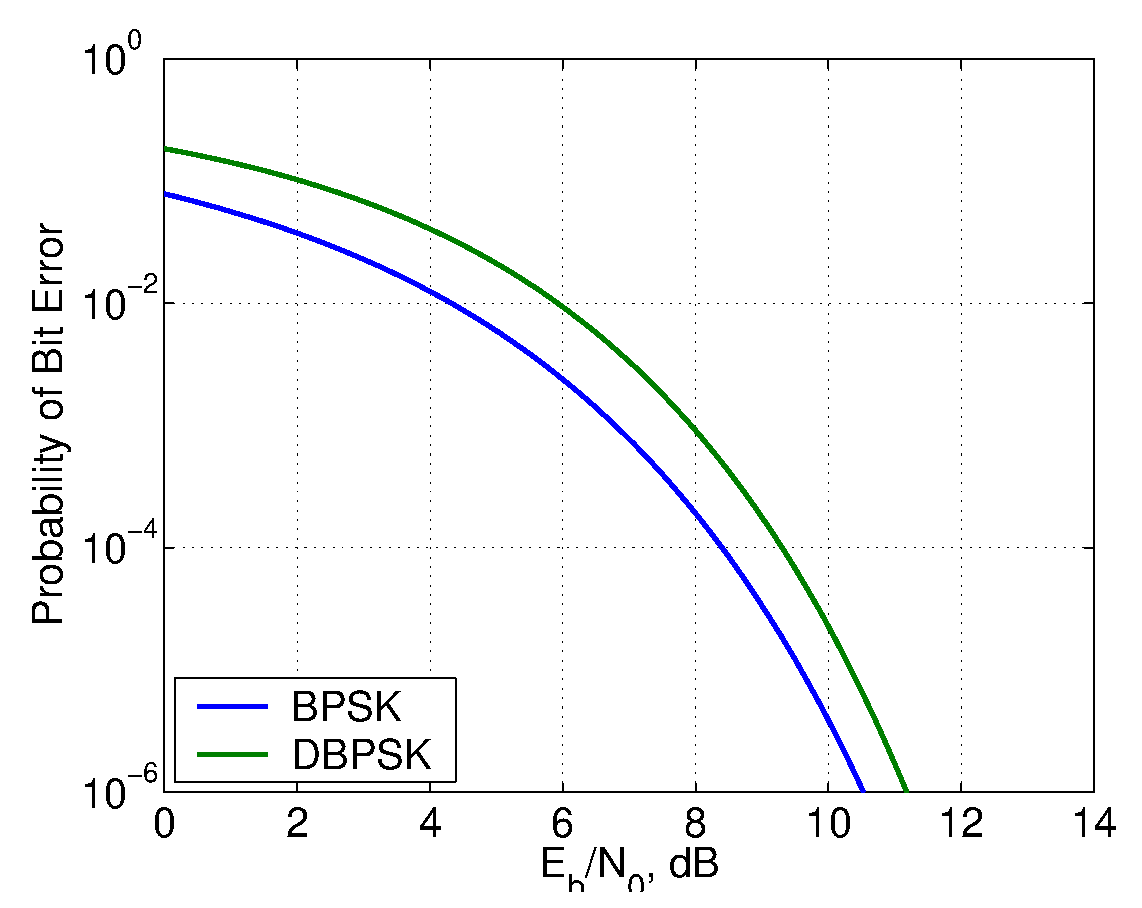
\includegraphics[width=0.65\textwidth]{../images/plotPbiterror_DPSK.eps}}
  \caption{Comparison of probability of bit error for BPSK and Differential BPSK.}
  \label{F:bpsk_vs_dpsk}
\end{figure}


 
\StartOf{Lecture 15}

\Today{(1) $M>2$ FSK Prob.\ Error, (2) Modulation Comparison}

\announcements{
}

\section{$M$-ary FSK Probability of Error}

\subsection{$M$-ary Non-Coherent FSK}

For $M$-ary non-coherent FSK, the derivation in the Proakis \& Salehi book, section 7.6.9, provides an exact expression for the probability of error in $M$-ary FSK.  The result is that
\[
\PR{\mbox{symbol error}} = \sum_{n=1}^{M-1} (-1)^{n+1} {M-1 \choose
n} \frac{1}{n+1} e^{-\log_2 M \frac{n}{n+1}\Ebno},
\]
and
\[
  \PR{\mbox{error}}_{M-nc-FSK} = \frac{M/2}{M-1}\PR{\mbox{symbol error}}.
\]
See Figure \ref{F:BER_NCFSK_Mary}.

\textit{Proof Summary}:  Our non-coherent receiver finds the energy in each frequency.  These energy values no longer have a Gaussian distribution (due to the squaring of the amplitudes in the energy calculation).  They instead are either Rician (for the transmitted frequency) or Rayleigh distributed (for the ``other'' $M-1$ frequencies).  The probability that the correct frequency is selected is the probability that the Rician random variable is larger than all of the other random variables measured at the other frequencies.

\begin{figure}[htbp]
  \centerline{\includegraphics[width=3in]{../images/plotBER_NCFSK_Mary.eps} }
  \caption{Probability of bit error for non-coherent reception of M-ary FSK.}
  \label{F:BER_NCFSK_Mary}
\end{figure}

\Example{Probability of Error for Non-coherent $M=2$ case}  Use the
above expressions to find the $\PR{\mbox{symbol error}}$ and
$\PR{\mbox{error}}$ for binary non-coherent FSK.

\Solution{
\[
\PR{\mbox{symbol error}} =  \PR{\mbox{bit error}} =
\frac{1}{2}e^{-\frac{1}{2}\Ebno}
\]
}

\subsection{$M$-ary FSK Coherent Receiver}

\begin{figure}
    \centering
    \includegraphics[width=0.5\textwidth]{../images/FSK-signalSpaceDiagram.eps}
    \caption{Constellation for $M=2$, $M=3$ FSK.}
    \label{F:FSK_constellation}
\end{figure}

For $M$-ary FSK with $M>2$, we don't have an exact expression for the probability of symbol error.  Instead, we use the union bound.  How many neighbors does each symbol have?  You can the constellation visually when $M=2$ or $M=3$ (in Figure \ref{F:FSK_constellation}).  For $M>3$, consider plotting any three dimensions of the constellation, and one of the three axes is symbol 0. You can see that both other symbols contribute a plane that contributes to the decision region of the symbol 0.  This is true regardless of which other symbols were chosen.  Thus each symbol has $M-1$ neighbors! 

The distance between neighbors is always $d=\sqrt{2}A$, and the average energy per symbol is $\En_s = A^2$, which means that $\En_b = A^2 / \log_2 M$.  Thus:
\begin{equation}
    \PR{\mbox{symbol error}} \le 
      (M-1) \Q{ \sqrt{\log_2 M \frac{\En_b }{N_0}}}
\end{equation}

Note however that one cannot do Gray encoding on the bits assigned to the $M$ symbols.  For symbol $i$, all $M-1$ other symbols are neighbors to it, and they are all equally distant from $i$.  Thus when a symbol error is made, it is equally likely to be to symbol $j\neq i$.  What is the average number of bit errors made when a symbol error is made?  

The Proakis \& Salehi book provides a derivation for the result, which is:
\begin{equation}
    \PR{\mbox{bit error}} = 
      \frac{M/2}{M-1} \PR{\mbox{symbol error}} 
    \le 
      \frac{M}{2} \Q{ \sqrt{(\log_2 M) \frac{\En_b }{N_0}}}.
\end{equation}

Here is a short argument about why we get the result we see in the Proakis \& Salehi handout: If I randomly pick any symbol, it will have $(\log_2 M)/2$ bit errors per symbol.  However, this includes the correct symbol.  Since we need to exclude the correct symbol, we need to multiply by a factor of $M/(M-1)$, that is $\frac{M\log_2 M}{(M-1) 2}$ bit errors per symbol.  Next, because this is the number of bit errors per symbol, we divide by $\log_2 M$ to get the number of bit errors per bit.  That is, $\frac{M/2}{M-1}$.


\section{Fidelity Comparison: $\PR{\mbox{error}}$ vs.~$\Ebno$}


Main modulations which we have evaluated probability of error vs.
$\Ebno$:
\begin{enumerate}
  \item M-ary PAM, including Binary PAM or BPSK, OOK, DPSK.
  \item M-ary PSK, including QPSK.
  \item Square QAM
  \item Non-square QAM constellations
  \item FSK, M-ary FSK
\end{enumerate}

In this part of the lecture we will break up into groups and
derive: (1) the probability of error and (2) probability of symbol
error formulas for these types of modulations.

\begin{table}
\begin{tabular}{|l|cc|}
\hline
 \bf Name & \bf $\PR{\mbox{symbol error}}$ & \bf $\PR{\mbox{bit error}}$ \\
\hline
 BPSK & $=\Q{ \sqrt{\frac{2\En_b }{N_0}}}$ & same \\
 OOK  & $=\Q{ \sqrt{\frac{\En_b }{N_0}}}$ & same \\
 DPSK & $=\frac{1}{2} \exp\left( -\Ebno \right)$ & same \\
 M-PAM & $= \frac{2(M-1)}{M} \Q{\sqrt{\frac{6 \log_2 M}{M^2-1} \frac{\En_b}{N_0}}}$ & 
         $\approx \frac{1}{\log_2 M} \PR{\mbox{symbol error}}$\\
 QPSK &  & $=\Q{ \sqrt{\frac{2\En_b }{N_0}}}$ \\
 M-PSK &  $\le 2 \Q{\sqrt{2 (\log_2 M)\sin^2(\pi/M) \frac{\En_b }{N_0}}}$  & $\approx \frac{1}{\log_2 M} \PR{\mbox{symbol error}}$ \\
% 4-PSK &  $\le 2 \Q{\sqrt{2  \frac{\En_b }{N_0}}}$  & $\approx \frac{1}{\log_2 M} \PR{\mbox{symbol error}}$ \\
 Square M-QAM &  & 
         $\approx \frac{4}{\log_2 M} \frac{(\sqrt{M}-1)}{\sqrt{M}} \Q{\sqrt{\frac{3 \log_2 M}{M-1} \frac{\En_b}{N_0}}}$ \\
 2-non-co-FSK & $=\frac{1}{2} \exp \left[- \frac{\En_b}{2N_0} \right]$ & same \\
 M-non-co-FSK & $=\sum_{n=1}^{M-1}  ({M-1 \atop n})  \frac{(-1)^{n+1}}{n+1} \exp \left[ -\frac{n \log_2 M}{n+1} \Ebno\right]$ 
              & $= \frac{M/2}{M-1} \PR{\mbox{symbol error}}$ \\  % \left( \begin{array}{c} M-1 \\  n \end{array} \right)
 2-co-FSK & $=\Q{\sqrt{\frac{\En_b}{N_0}}}$ & same \\
 M-co-FSK & $\le (M-1) \Q{ \sqrt{\log_2 M \frac{\En_b }{N_0}}}$ 
              & $= \frac{M/2}{M-1} \PR{\mbox{symbol error}}$ \\
\hline
\end{tabular}
\caption{Summary of probability of bit and symbol error formulas for several modulations.}
\end{table}  


See also Rice Section 6.3



\subsection{Bandwidth Efficiency Comparison}

We've talked about measuring data rate in bits per second. We've
also talked about Hertz, \ie, the quantity of spectrum our signal
will use.  Typically, we can scale a system, to increase the bit
rate by decreasing the symbol period, and correspondingly increase
the bandwidth.  These two have a linear proportional relationship.

\Definition{Bandwidth efficiency}{ The bandwidth efficiency, typically denoted $\eta$, is the ratio of bits per second to bandwidth:
\[
  \eta = R_b/B_T
\]
}
Bandwidth efficiency depends on the definition of ``bandwidth''.  Since it is usually used for comparative purposes, we just make sure we use the same definition of bandwidth throughout a comparison.

The key figure of merit:  bits per second / Hertz, \ie, bps/Hz.

\subsubsection{PSK, PAM and QAM}

In these three modulation methods, the bandwidth is largely
determined by the pulse shape.  For root raised cosine filtering,
the null-null bandwidth is $1+\alpha$ times the bandwidth of the
case when we use pure sinc pulses.  The transmission bandwidth (for
a bandpass signal) is
\[
  B_T = \frac{1+\alpha}{T_{s}}
\]
Since $T_{s}$ is seconds per symbol, we divide by $\log_2 M$ bits
per symbol to get $T_b = T_{s} / \log_2 M$ seconds per bit, or
\[
  B_T = \frac{(1+\alpha)R_b}{\log_2 M}
\]
where $R_b = 1/ T_b$ is the bit rate.

Bandwidth efficiency is then
\[
  \eta = R_b/B_T = \frac{\log_2 M}{1+\alpha}
\]
See Table \ref{T:BW_Efficiency} for some numerical examples.

\begin{table}
  \centering
\begin{tabular}{|l|ccc|}
  \hline
  $\eta$ & $\alpha=0$ & $\alpha=0.5$ & $\alpha=1$ \\
  \hline
  BPSK   & 1.0        & 0.67         & 0.5 \\
  QPSK   & 2.0        & 1.33         & 1.5 \\
  16-QAM & 4.0        & 2.67         & 2.0 \\
  64-QAM & 6.0        & 4.0          & 3.0 \\
  \hline
\end{tabular}
  \caption{Bandwidth efficiency of PSK and QAM modulation methods
  using raised cosine filtering as a function of $\alpha$.}\label{T:BW_Efficiency}
\end{table}


\subsubsection{FSK}

We've said that the bandwidth of FSK is,
\[
B_T = (M-1) \Delta f + 2B
\]
where $B$ is the one-sided bandwidth of the digital baseband signal.
For the null-to-null bandwidth of  raised-cosine pulse shaping,
$2B=(1+\alpha)/T_{s}$. So,
\[
B_T = (M-1) \Delta f + (1+\alpha)/T_{s} = \frac{R_b}{\log_2 M}
\left\{(M-1)\Delta f T_{s} + (1+\alpha) \right\}
\]
since $R_b = 1/T_{s}$ for
\[
  \eta = R_b/B_T = \frac{\log_2 M}{(M-1)\Delta f T_{s} + (1+\alpha)}
\]
If $\Delta f = 1/T_s$ (required for non-coherent reception),
\[
  \eta = \frac{\log_2 M}{M+\alpha}
\]


\subsection{Bandwidth Efficiency vs.~$\Ebno$}

For each modulation format, we have quantities of interest:
\begin{itemize}
  \item Bandwidth efficiency, and
  \item Energy per bit ($\Ebno$) requirements to achieve a given
  probability of error.
\end{itemize}

\Example{Bandwidth efficiency vs.~$\Ebno$ for $M=8$ PSK} What is the
required $\Ebno$ for 8-PSK to achieve a probability of bit error of
$10^{-6}$?  What is the bandwidth efficiency of 8-PSK when using
50\% excess bandwidth?

\Solution{Given in Rice Figure 6.3.5 (Figure 6.13?) to be about 14 dB, and 2.}

We can plot these (required $\Ebno$, bandwidth efficiency) pairs.
 See Rice Figure 6.3.6.
 
\StartOf{Lecture 16}

\Today{(1) Received Power Models, (2) Noise Energy, (3) Link Budgeting}

\announcements{
\begin{itemize}
  \item Today's reading: Rice 6.4.  
\end{itemize}
}

\section{Noise and Received Power Models}

This section starts to make the connection between the energy per bit which we use in probability of error formulas to the transmit power and distance between the transmitter and receiver in a given communication system.  Given that we want our wireless communication system to operate in some application or for some link, how can we calculate how much power will be received, typically?  We do this here for both wireless and wired channels.  Wireless channels we divide into free space channels, and obstructed (non-free-space channels).  My research and experience is in the design of wireless systems, so I must warn you that I provide much more detail for wireless than for wired communication systems.

\subsection{Free Space}

`Free space' is the idealization in which nothing exists except for
the transmitter and receiver, and can really only be used for deep space
communications.  But, this formula serves as a starting point for other
radio propagation formulas.  In free space, the received power is calculated from
the Friis formula,
\[
C = P_R = P_T G_T G_R \left(\frac{ \lambda}{4\pi R_0}\right)^2 
\left( \frac{ R_0}{R}\right)^2
\]
where
\begin{itemize}
  \item $G_T$ and $G_R$ are the antenna gains at the transmitter and
  receiver, respectively.
  \item $P_T$ is the transmit power.
  \item $\lambda$ is the wavelength at signal frequency.
  For narrowband signals, the wavelength is nearly constant across
  the bandwidth, so we just use the center frequency $f_c$.  Note
  that $\lambda = c / f_c$ where $c = 3\times 10^8$ meters per
  second is the speed of light.
  \item $R_0$ is a reference distance, say 1 meter or 10 meters. You may notice that the $R_0$s cancel, so why have I put it in?  It is useful for understanding the relationships and for keeping track of the units. 1) One can measure the received power at a reference distance $R_0$ during testing, and then replace the $P_T G_T G_R \left(\frac{ \lambda}{4\pi R_0}\right)^2$ part with the measurement; 2) Each fraction has units that cancel; and 3) We consider the $\left( \frac{ R_0}{R}\right)^2$ part as the \emph{path loss}, i.e., loss due to the actual path length (distance between the transmitter and receiver).
\end{itemize}
Here, everything is in linear terms.  Typically people use decibels
to express these numbers, and we will write $\dBm{P_R}$ or
$\dB{G_T}$ to denote that they are given by:
\begin{eqnarray}
  \dBm{P_R}  &=& 10 \log_{10} P_R \nnn
  \dB{G_T} &=& 10 \log_{10} G_T \nnn
\end{eqnarray}

The Friis formula, given in dB, is
\begin{equation} \label{E:FriisIndB}
 \dBm{C} = \dB{G_T} + \dB{G_R}  + \dBm{P_T} + 20 \log_{10} \frac{\lambda}{4\pi R_0} - 20 \log_{10} \frac{R}{R_0} 
\end{equation}
This says the received power, $C$, is linearly proportional to the log of the distance $R$.  

The received power at the reference distance $R_0$ is called $\dBm{P_0}$ and is given by:
\begin{equation} \label{E:P0_formula}
 \dBm{P_0} = \dB{G_T} + \dB{G_R}  + \dBm{P_T} + 20 \log_{10} \frac{\lambda}{4\pi R_0}
\end{equation}
Again, $\dBm{P_0}$  is something you might measure with a well-calibrated receiver and an antenna.  If you know (or estimate) $\dBm{P_0}$, then the relationship of received power (dBm) with distance $R$ is simply:
\begin{equation} \label{E:FriisIndBSimple}
 \dBm{C} = \dBm{P_0} - 20 \log_{10} \frac{R}{R_0} .
\end{equation}


%The Rice book writes the Friis formula as
%\[
% \dBm{C} = \dB{G_T} + \dB{G_R}  + \dBm{P_T} + \dB{L_p}
%\]
%where 
%\[
% \dB{L_p} = + 20 \log_{10} \frac{\lambda}{4\pi} - 20 \log_{10} R 
%\]
%where $\dB{L_p}$ is called the ``channel loss''.  (This name that Rice chose is unfortunate because if it was positive, it would be a ``gain'', but it is typically very negative.  My opinion is, it should be called ``channel gain'' and have a negative gain value.)

There are also typically other losses in a transmitter / receiver system; losses in a cable, other imperfections, etc.  In the Rice book, these are labelled as $L$[dB]. You must subtract the dB loss from the left-hand side of (\ref{E:FriisIndB}):
\begin{equation} \label{E:FriisIndBSimpleLoss}
 \dBm{C} = \dBm{P_0} - 20 \log_{10} \frac{R}{R_0} -\dB{L}.
\end{equation}
Note that you need to be careful (because Rice is not) that if you call it a dB ``loss'', it is positive value that you subtract from (\ref{E:FriisIndBSimple}), but you if you call it a ``gain'' than it must be subtracted from (\ref{E:FriisIndBSimple}).



\subsection{Non-free-space Channels}

We don't study radio propagation path loss formulas in this course.  But, a very short summary is that radio propagation on Earth is different than the Friis formula suggests. Lots of other formulas exist that approximate the received power as a function of distance, antenna heights, type of environment, etc.  The main problem is that walls, trees, buildings, and terrain decrease the power that would be received as compared to the Friis model.  This is called ``shadowing'' in analogy to how objects shadow light.

The most common model for real world shadowing effects is the path loss exponent model, in which received power (dBm) is linear with the log of distance,
\begin{equation} \label{E:PLExponentModel}
  \dBm{C} = \dBm{P_0} - 10n_p \log_{10}\frac{R}{R_0},
\end{equation}
for some constant $n_p$. Here, $\dBm{P_0}$ is typically the same as we described earlier, that is, the path loss that the Friis model would predict at some short distance $R_0$ from the antenna.  Usually $R_0$ is a very short distance, like $1$ m or $10$ m. Effectively, because of shadowing caused by buildings, trees,
etc., the average loss may increase more quickly than $1/R^2$, instead, it may be more like $1/R^{n_p}$.  

Equivalently, in linear terms:
\[
C = P_R = P_T G_T G_R \left(\frac{ \lambda}{4\pi R_0}\right)^2 
\left( \frac{ R_0}{R}\right)^{n_p}
\]


This is a model that comes with lots of evidence from empirical measurement studies.  In dense urban areas like Manhattan, people observe a much higher $n_p$ than in rural areas.  In mountainous areas, we typically observe a higher $n_p$ than in flat areas.  When the antennas are both close to the ground, the $n_p$ is higher than when the antennas are held tens of meters away from the ground.  Finally, in buildings, we observe a higher $n_p$ when the walls are made of bricks or concrete, than when the walls are drywall and wood frame.  The value of $n_p$ may range from 2 to 4.5, with some values going lower than 2 or higher than 4.5.  In real life, you would want to measure $n_p$ in the type of environment you want to have your link operate in, or use values from the literature on measurement-based path loss models.

However, note that (\ref{E:PLExponentModel}) is only the \emph{average} received power.  In reality, any one particular measurement of received power a distance $R$ from the transmitter may be off by 10-30 dB from the average, due to differences in the particular path that the signal travels, due to small-scale fading, and for other reasons.


\subsection{Wired Channels}

Typically wired channels are lossy as well, but the loss is modeled as linear in the length of the cable.  For example, 
\[
 \dBm{C} = \dBm{P_T} - R (\dB{L_{1m}})
\]
where $P_T$ is the transmit power and $R$ is the cable length in meters, and $L_{1m}$ is the loss per meter.  


\subsection{Noise Energy}

The noise energy $N_0$ can be calculated as:
\[
N_0 = kT_{eq}
\]
where $k = 1.38 \times 10^{-23}$ J/K is Boltzmann's constant and $T_{eq}$ is
called the equivalent noise temperature in Kelvin.  This is a topic covered in
another course, and so you are not responsible for that material
here.  But in short, the equivalent temperature is a function of the receiver design, and $T_0$, the temperature of the environment at which the antenna is receiving from.  
$T_{eq}$ is always going to be higher than $T_0$.  Basically, all receiver circuits add
noise to the received signal.  With proper design (and more expensive and power-hungry components), $T_{eq}$ can be kept low.  






\section{System Design}
This section makes connections between the modulation performance formulas we've already discussed to the received power models just mentioned, in order to analyze a system design. 

For example, we may want to figure out what modulation, bit rate, and transmit power to use for a deep space communication system.  Or for a new long-range IoT system.  Or for a fiber-optic communications system.  You may find that you need several missing (or forgotten) connections to other topics in order to design a real-world communication system.  This lecture and the next lecture are designed to present these connections. 

As a digital communication system designer, your mission (if you choose to accept it) is to achieve:
\begin{enumerate}
 \item High data rate
 \item High fidelity (low bit error rate)
 \item Low transmit power 
 \item Low bandwidth
 \item Low transmitter/receiver complexity
 \item Long range
\end{enumerate}
But this is truly a mission impossible, because you can't have everything at the same time.  So the system design depends on what the desired system really needs and what are the acceptable trade-offs.  Typically some subset of requirements are given; for example, given the bandwidth limits, the received signal power and noise power, and bit error rate limit, what data rate can be achieved?  Using which modulation?

\section{Using the Relationship Flow Chart}

For a typical system design question, we are given some constraints (at the given limits) and asked to determine other system parameters.  For these types of problems I find it helpful to use the flow chart in Figure \ref{F:RelationshipsFlowChart} to keep track of my given constraints, the many functional relationships that exist in wireless communication system design, and thus how to get to the parameter of interest.  

In this lecture, we discuss this procedure, and define each of the variables we see in Figure \ref{F:RelationshipsFlowChart}, and to what they are related.  This lecture is about system design, and it cuts across electrical and computer engineering classes; in particular circuits, radio propagation, antennas, optics, and the material from this class.  You are expected to apply what you have learned in other classes (or learn the functional relationships that we describe here).

\begin{figure}[htbp]
    \includegraphics[width=6.5in]{../images/relationshipGraphDigiComm.eps}
    \caption{Relationships between important system design variables (rectangular boxes).  Functional relationships between variables are given as circles, with   division ($\div$), multiplication ($\times$), or another more complicated function $f()$. For example, $C/N_0$ is shown to have a divide by relationship with $C$ and $N_0$.  The effect of the choice of modulation impacts several functional relationships, \eg, the relationship between probability of bit error and $\Ebno$, which is drawn as a dotted line.}
    \label{F:RelationshipsFlowChart}
\end{figure}

\subsection{Link Budgets Given $C/N_0$}

The received power is denoted $C$, it has units of Watts.  What is $C/N_0$?  It is received power divided by noise energy.  It is a nebulous quantity, but it summarizes what we need to know about the signal and the noise for the purposes of system design.  
\begin{itemize}
%
 \item We (and other books) often describe both the received power as $P_R$, but in the Rice book it is typically denoted $C$.
%
 \item We know the probability of bit error is typically written as a function of $\Ebno$.  The noise energy is $N_0$.  The bit energy is $\En_b$.  We can write $\En_b = C T_b$, since energy is power $\times$ time.
To separate the effect of $T_b$, we often denote:
\[
  \Ebno = \frac{C}{N_0} T_b = \frac{C/N_0}{R_b}
\]
where $R_b = 1/T_b$ is the bit rate.  In other words, $C/N_0 = \Ebno   R_b$   What are the units of $C/N_0$? {\it Answer: Hz, 1/s}.  
 \item Note that people often report $C/N_0$ in dB Hz, which is
  \[
    10 \log_{10} \frac{C}{N_0}
  \]
%
 \item Be careful of Bytes (B) per second vs bits (b) per second.  Commonly, computer science 
people use Bps (kBps or MBps) when describing data rate.  For
example, if it takes 5 seconds to transfer a 1MB file, then software
often reports that the data rate is $1/5=0.2$ MBps or 200 kBps. But
the bit rate is $8/5$ Mbps or $1.6\times 10^6$ bps.  This number is $8\times$ larger so it is the one used by your ISP when selling you your internet service!
%
\end{itemize}

Given $C/N_0$, we can now relate bit error rate, modulation, bit rate, and bandwidth.

\Note{  
 We typically use $\Q{\cdot}$ and $\Qinv{\cdot}$ to relate BER and $\Ebno$ in each direction.  
 While you have Matlab, this is easy to calculate.  If you can program it into your 
 calculator, great.  Otherwise, it's really not a big deal to pull it 
 off of a chart or table.  For your convenience, the following tables/plots 
 of $\Qinv{x}$ will appear on Exam 2.  I am not picky about getting lots 
 of correct decimal places.}

\newpage
\centerline{ TABLE OF THE $\Qinv{\cdot}$ FUNCTION: }
\begin{tabular}{|l|l|l|}
  \hline
$\Qinv{1\times 10^{-6}} =  4.7534$ & $\Qinv{1\times 10^{-4}} =  3.719$ & $\Qinv{1\times 10^{-2}} =  2.3263$ \\
$\Qinv{1.5\times 10^{-6}} =  4.6708$ & $\Qinv{1.5\times 10^{-4}} =  3.6153$ & $\Qinv{1.5\times 10^{-2}} =  2.1701$ \\
$\Qinv{2\times 10^{-6}} =  4.6114$ & $\Qinv{2\times 10^{-4}} =  3.5401$ & $\Qinv{2\times 10^{-2}} =  2.0537$ \\
$\Qinv{3\times 10^{-6}} =  4.5264$ & $\Qinv{3\times 10^{-4}} =  3.4316$ & $\Qinv{3\times 10^{-2}} =  1.8808$ \\
$\Qinv{4\times 10^{-6}} =  4.4652$ & $\Qinv{4\times 10^{-4}} =  3.3528$ & $\Qinv{4\times 10^{-2}} =  1.7507$ \\
$\Qinv{5\times 10^{-6}} =  4.4172$ & $\Qinv{5\times 10^{-4}} =  3.2905$ & $\Qinv{5\times 10^{-2}} =  1.6449$ \\
$\Qinv{6\times 10^{-6}} =  4.3776$ & $\Qinv{6\times 10^{-4}} =  3.2389$ & $\Qinv{6\times 10^{-2}} =  1.5548$ \\
$\Qinv{7\times 10^{-6}} =  4.3439$ & $\Qinv{7\times 10^{-4}} =  3.1947$ & $\Qinv{7\times 10^{-2}} =  1.4758$ \\
$\Qinv{8\times 10^{-6}} =  4.3145$ & $\Qinv{8\times 10^{-4}} =  3.1559$ & $\Qinv{8\times 10^{-2}} =  1.4051$ \\
$\Qinv{9\times 10^{-6}} =  4.2884$ & $\Qinv{9\times 10^{-4}} =  3.1214$ & $\Qinv{9\times 10^{-2}} =  1.3408$ \\
\hline
$\Qinv{1\times 10^{-5}} =  4.2649$ & $\Qinv{1\times 10^{-3}} =  3.0902$ & $\Qinv{1\times 10^{-1}} =  1.2816$ \\
$\Qinv{1.5\times 10^{-5}} =  4.1735$ & $\Qinv{1.5\times 10^{-3}} =  2.9677$ & $\Qinv{1.5\times 10^{-1}} =  1.0364$ \\
$\Qinv{2\times 10^{-5}} =  4.1075$ & $\Qinv{2\times 10^{-3}} =  2.8782$ & $\Qinv{2\times 10^{-1}} =  0.84162$ \\
$\Qinv{3\times 10^{-5}} =  4.0128$ & $\Qinv{3\times 10^{-3}} =  2.7478$ & $\Qinv{3\times 10^{-1}} =  0.5244$ \\
$\Qinv{4\times 10^{-5}} =  3.9444$ & $\Qinv{4\times 10^{-3}} =  2.6521$ & $\Qinv{4\times 10^{-1}} =  0.25335$ \\
$\Qinv{5\times 10^{-5}} =  3.8906$ & $\Qinv{5\times 10^{-3}} =  2.5758$ & $\Qinv{5\times 10^{-1}} =  0$ \\
$\Qinv{6\times 10^{-5}} =  3.8461$ & $\Qinv{6\times 10^{-3}} =  2.5121$ &  \\
$\Qinv{7\times 10^{-5}} =  3.8082$ & $\Qinv{7\times 10^{-3}} =  2.4573$ &  \\
$\Qinv{8\times 10^{-5}} =  3.775$ & $\Qinv{8\times 10^{-3}} =  2.4089$ &  \\
$\Qinv{9\times 10^{-5}} =  3.7455$ & $\Qinv{9\times 10^{-3}} =  2.3656$ &  \\
\hline
\end{tabular}


\includegraphics[width=5.5in]{../images/plotQinv.eps}






\subsection{Examples}

\Example{Rice 6.36}  

Consider a ``point-to-point'' microwave link. (Such links provide the internet backbone for cellular base stations and internet providers where fiber optic cables can't be installed, for example in rural areas.) Both antenna gains are 20 dB and the transmit antenna power is 10 W. The modulation is 51.84 Mbits/sec 256 square QAM with a carrier frequency of 4 GHz. Atmospheric losses are 2 dB and other incidental losses are 2 dB. A pigeon in the line-of-sight path causes an additional 2 dB loss. The receiver has an equivalent noise temperature of 400 K and an implementation loss of 1 dB. How far away can the two towers be if the bit error rate is not to exceed $10^{-8}$? Include the pigeon. 

Neal's hint: Use the dB version of Friis formula and subtract these mentioned dB losses: atmospheric losses, incidental losses, implementation loss, and the pigeon.

\Solution{
Starting with the modulation, $M=256$ square QAM ($\log_2 M = 8$, $\sqrt{M} = 16$), to achieve $\PR{\mbox{error}}=10^{-8}$,
\begin{eqnarray}
    10^{-8} &=& \frac{4}{\log_2 m} \frac{(\sqrt{M}-1)}{\sqrt{M}} \Q{\sqrt{\frac{3 \log_2 M}{M-1} \frac{\En_b}{N_0}}} 
  \nnn
    10^{-8} &=& \frac{4}{8} \frac{15}{16} \Q{\sqrt{\frac{3 (8)}{255} \frac{\En_b}{N_0}}} 
  \nnn
    10^{-8} &=& \frac{15}{32} \Q{\sqrt{\frac{24}{255} \frac{\En_b}{N_0}}} .
  \nnn
    \Ebno &=& \frac{255}{24} \left[ \Qinv{\frac{32}{15} 10^{-8} }\right]^2  = 319.0 \nn
\end{eqnarray}
The noise power $N_0 = kT_{eq} = 1.38\times 10^{-23} (\mbox{J/K}) 400   (\mbox{K}) = 5.52\times 10^{-21}$ J.  So 
$\En_b = 319.0 \times 5.52\times 10^{-21} = 1.76 \times 10^{-18}$ J.  Since $\En_b = C /R_b$ and the bit rate $R_b = 51.84 \times 10^6$ bits/sec,
$C = (51.84 \times 10^6) J (1.76 \times 10^{-18}) 1/sec = 9.13\times 10^{-11}$ W, or -100.4 dBW.

Switching to finding an expression for $C$, the wavelength is $\lambda = 3\times 10^8 \mbox{m/s} / 4\times 10^9 \mbox{1/s} = 0.075 m$, so:
\begin{eqnarray}
 \dBW{C} &=& \dB{G_T} + \dB{G_R}  + \dBW{P_T} + 20 \log_{10} \frac{\lambda}{4\pi} - 20 \log_{10} R - 2 \mbox{dB}- 2 \mbox{dB}- 2\mbox{dB} - 1\mbox{dB} 
   \nnn
         &=& 20 \mbox{dB} + 20 \mbox{dB} + 10 \mbox{dBW} + 20 \log_{10} \frac{0.075 m }{4\pi} - 20 \log_{10} R - 7 dB
   \nnn
         &=& -1.48 \mbox{dBW} - 20 \log_{10} R 
\end{eqnarray}
Plugging in $\dBm{C} = -100.4$ dBW $= -1.48 \mbox{dBW} - 20 \log_{10} R $ and solving for $R$,  we find $R = 88.3$ km.  Thus microwave towers should be placed at most 88.3 km (about 55 miles) apart.
}


  
\StartOf{Lecture 17}

\Today{(1) Link Budgeting}

\announcements{
\begin{itemize}
  \item Today's reading: Rice 6.4.  
\end{itemize}
}


\section{Link Budgeting}

The idea of this section is that system designs are not always straightforward solutions of the equations we have.  We may have constraints that are difficult to simultaneously meet, for example, on bandwidth and power.  To meet all constraints, we may need to be more restrictive than the constraint on one parameter in order to exactly meet the constraint on another.

\subsection{Bandwidth and Energy Limited Channels}

Assume the $C/N_0$, the maximum bandwidth, and the maximum BER are all given.  
Sometimes power is the limiting factor in determining the maximum
achievable bit rate. Such links (or channels) are called \emph{power
limited} channels. Sometimes bandwidth is the limiting factor in
determining the maximum achievable bit rate. In this case, the link
(or channel) is called a \emph{bandwidth limited} channel.  You just
need to try to solve the problem and see which one limits your
system.

Here is a step-by-step version of what you might need do in this case:

\textbf{Method A: Start with power-limited assumption:}
\begin{enumerate}
  \item Use the probability of error constraint to determine the
    $\Ebno$ constraint, given the appropriate probability of error
    formula for the modulation.
  \item Given the $C/N_0$ constraint and the $\Ebno$ constraint,
    find the maximum bit rate.  Note that $R_b = 1/T_b = \frac{C/N_0}{\Ebno}$,
    but be sure to express both in linear units.
  \item Given a maximum bit rate, calculate the maximum symbol rate
    $R_s = \frac{R_b}{\log_2 M}$ and then compute the required bandwidth
    using the appropriate bandwidth formula.
  \item  Compare the bandwidth at maximum $R_s$ to the bandwidth
    constraint:  If BW at $R_s$ is too high, then the system is
    bandwidth limited; reduce your bit rate to conform to the BW constraint.
    Otherwise, your system is power limited, and your $R_b$ is
    achievable.
\end{enumerate}

\textbf{Method B: Start with a bandwidth-limited assumption:
}\begin{enumerate}
  \item Use the bandwidth constraint and the appropriate bandwidth formula to find the maximum symbol
    rate $R_s$ and then the maximum bit rate $R_b$.
  \item Find the $\Ebno$ at the given bit rate by computing $\Ebno = \frac{C/N_0}{R_b}$.
    (Again, make sure that everything is in linear units.)
  \item Find the probability of error at that $\Ebno$, using  the appropriate probability of error
    formula.
  \item If the computed $\PR{\mbox{error}}$ is greater than the BER
    constraint, then your system is power limited.  Use the previous
    method to find the maximum bit rate.  Otherwise, your system is
    bandwidth-limited, and you have found the correct maximum bit rate.
\end{enumerate}


\Example{Rice 6.33}

Consider a bandpass communications link with a bandwidth of 1.5 MHz and with an available $C/N_0 = 82$ dB Hz. The maximum bit error rate is $10^{-6}$.
\begin{enumerate}
  \item If the modulation is 16-PSK using the SRRC pulse shape with $\alpha = 0.5$, what is the maximum achievable bit rate on the link? Is this a power limited or bandwidth limited channel?
  \item If the modulation is square 16-QAM using the SRRC pulse shape with $\alpha = 0.5$, what is the maximum achievable bit rate on this link? Is this a power limited or bandwidth limited channel?
\end{enumerate}

\Solution{
\begin{enumerate}
  \item Try Method A.  For $M=16$ PSK, we can find $\Ebno$ for the maximum BER:
\begin{eqnarray}
 10^{-6} &=& \PR{\mbox{error}} = \frac{2}{\log_2 M} \Q{\sqrt{2(\log_2 M)\sin^2(\pi/M) \frac{\En_b }{N_0}}}
   \nnn
 10^{-6} &=& \frac{2}{4} \Q{\sqrt{2(4) \sin^2(\pi/16)  \frac{\En_b }{N_0}}}
   \nnn
 \frac{\En_b }{N_0} &=& \frac{1}{8 \sin^2(\pi/16)}\left[\Qinv{2\times 10^{-6}}\right]^2
    \nnn
 \frac{\En_b }{N_0} &=& 69.84 
\end{eqnarray}
Converting $C/N_0$ to linear, $C/N_0 = 10^{82/10} = 1.585\times 10^{8}$.  Solving for $R_b$,
\[
  R_b = \frac{C/N_0}{\Ebno} = \frac{1.585\times 10^{8}}{69.84} = 2.27\ep{6} = 2.27 \mbox{ Mbits/s}
\]
and thus $R_s= R_b/\log_2 M = 2.27\ep{6}/4 = 5.67\ep{5} \mbox{ Msymbols/s}$.  The required bandwidth for this system is
\[
 B_T = \frac{(1+\alpha)R_b}{\log_2 M} = 1.5(2.27\ep{6}) / 4 = 851 \mbox{ kHz}
\]
This is clearly lower than the maximum bandwidth of 1.5 MHz.  So, the system is power limited, and can operate with bit rate 2.27 Mbits/s.
(If $B_T$ had come out $> 1.5$ MHz, we would have needed to reduce $R_b$ to meet the bandwidth limit.)
%
  \item Try Method A.  For $M=16$ (square) QAM, we can find $\Ebno$ for the maximum BER:
\begin{eqnarray}
 10^{-6} &=& \PR{\mbox{error}} = \frac{4}{\log_2 M} \frac{(\sqrt{M}-1)}{\sqrt{M}} \Q{\sqrt{\frac{3 \log_2 M}{M-1} \frac{\En_b}{N_0}}}
   \nnn
 10^{-6} &=& \frac{4}{4} \frac{(4-1)}{4} \Q{\sqrt{\frac{3 (4)}{15} \frac{\En_b}{N_0}}}
   \nnn
 \frac{\En_b }{N_0} &=& \frac{15}{12}\left[\Qinv{(4/3)\times 10^{-6}}\right]^2
    \nnn
 \frac{\En_b }{N_0} &=& 27.55
\end{eqnarray}
Solving for $R_b$,
\[
  R_b = \frac{C/N_0}{\Ebno} = \frac{1.585\times 10^{8}}{27.55} = 5.75\ep{6} = 5.75 \mbox{ Mbits/s}
\]
The required bandwidth for this bit rate is:
\[
 B_T = \frac{(1+\alpha)R_b}{\log_2 M} = 1.5(5.75\ep{6}) / 4 = 2.16 \mbox{ MHz}
\]
This is greater than the maximum bandwidth of 1.5 MHz, so we must reduce the bit rate to 
\[
R_b = \frac{B_T \log_2 M}{1+\alpha} = 1.5 \mbox{ MHz} \frac{4}{1.5} = 4\mbox{ MHz}
\]
In summary, we have a bandwidth-limited system with a bit rate of 4 MHz.
%
\end{enumerate}
}

% Part 1 is power limited.  Use method A to see that it can
% achieve a rate of about 2.27 Mbps.  Part 2 is bandwidth limited.
% From method B, it is seen that it can achieve a bit rate of 4 Mbps.}


\subsection{Link Budget Spreadsheet}

I've shared a Google sheet that I use to calculate probability of error quickly for many different modulations:
\begin{verbatim}
    https://bit.ly/LinkBudgetSheet
\end{verbatim}

On one sheet, you may enter the TX/RX parameters, starting from the right side of the relationship diagram (Figure 1 in Lecture 16), and calculating the bandwidth and probability of bit error.  On the second sheet, you start with the probability of bit error and $C/N_0$ ratio and it calculates the bit rate and bandwidth.

The sheet is linked to from the schedule table on Canvas.  Please save a copy for yourself, modify parameters, and see that the changes go in the direction that you expect.  You may use this to check your answer while doing homework, but please do the calculations yourself so that you have practice.  

If you're interested in how I made the sheet work, please inspect the code I inserted for the $Q()$ function and $Q^{-1}()$ function by going to  Tools:Script Editor; this is handy whenever your function is not a standard spreadsheet function.

\StartOf{Lecture 18}

\Today{(1) Source Coding \& Entropy, (2) Joint / Conditional Entropy, (3) Entropy Rate, (4) Source Coding Theorem}

\announcements{
\begin{itemize}
  \item Today's reading: Claude E. Shannon, ``A Mathematical Theory of Communication'', \emph{The Bell System Technical Journal}, 1948.  Read Part I.
\end{itemize}
}

\section{Source Coding}

We talk in this course quite a bit about ``bits'', the fundamental measure of the information we're designing a communication system to send.  The purpose of today's lecture is to describe what a \emph{bit rate} really means when we know what kind of data will be sent (a.k.a. our ``source'').  The short story is, when we do know about the data being sent, that the data rate we need to send is \emph{at least} the \emph{entropy rate} of the data, which is a quantity that can be determined from the statistics of the data.

This topic is a semester-long course at the graduate level in
itself; but the basic ideas can be presented pretty quickly.  Claude Shannon presented an introduction to source coding in Part 1 of his 1948 paper, ``A mathematical theory of communication'' \cite{shannon1948mathematical}, which introduced the concept.

We have done a lot of counting of bits as our primary measure of
communication systems.  Our information source is measured in bits,
or in bits per second.  Modulation schemes' bandwidth efficiency is
measured in bits per Hertz, and energy efficiency is energy per bit
over noise PSD.  Lots of what a communication engineer does is measured in bits!

But how do we measure the bits of a source (\eg, audio, video, email, SMS, $\ldots$)?  Information can often be represented in many different ways. Images and sound can be encoded in different ways.  Text files can be presented in different ways.

Here are two misconceptions:
\begin{enumerate}
  \item The file size tells you how much information is contained within the file.
  \item The number of bits is the $\log_2$ of the number of different values the data could possibly send.
\end{enumerate}

For example, consider a digital black \& white image (not grayscale, in this example, truly black or white).
\begin{enumerate}
  \item You could store it as the value for each pixels.  Each pixel has two
  possibilities (possible values),
  thus we could encode it in $\log_2 2 = 1$ bit per pixel.
  \item You could simply send the coordinates of the pixels of one
  of the colors (\eg all black pixels).
\end{enumerate}
How many bits would be used in these two representations? What would
make you decide which one is more efficient?

\vspace{0.05in} \noindent  From this example, two equivalent representations could require a different number of bits.  This is the idea behind \emph{source compression}. For example, .zip or .tar files represent the exact same information that was contained in the original files, but with fewer bits.

\vspace{0.05in} \noindent  What if we had a fixed number of bits to
send any image, and we used the sparse B\&W image coding scheme (2.)
above?  Sometimes, the number of bits in the compressed image would
exceed what we had allocated.  This would introduce errors into the
image.

Two types of compression algorithms:
\begin{itemize}
  \item Lossless: \eg, Zip or compress.
  \item Lossy:  \eg, JPEG, MP3, MP4
\end{itemize}

\Note{Both ``zip'' and the linux ``compress'' commands use the
Lempel-Ziv algorithm for source compression.}

So what is the intrinsic measure of bits of text, an image, audio, or video?

\subsection{Entropy}

Entropy is a measure of the randomness of a random variable (r.v.).
\emph{Randomness} and \emph{information}, in non-technical language,
are just two perspectives on the same thing:
\begin{itemize}
  \item If you are told the value of a r.v.\ that doesn't vary that
    much, that telling conveys very little information to you.
  \item If you are told the value of a very ``random'' r.v., that
    telling conveys quite a bit of information to you.
\end{itemize}

Our technical definition of entropy of a discrete random variable is as
follows.

\Definition{Entropy}{ Let $X$ be a discrete random variable with pmf
$p_X(x_i) = \PR{X=x}$.  Here, there is a finite or countably
infinite set $S_X$, and $x \in S_X$.   We will shorten the notation
by using $p_i$ as follows:
\[
  p_i = p_X(x_i) = \PR{X=x_i}
\]
where $\{x_1, x_2, \ldots\}$ is an ordering of the possible values
in $S_X$. Then the entropy of $X$, in units of bits, is defined as,
\begin{equation} \label{E:Entropy}
  \entropy{X} = -\sum_i p_i \log_2 p_i   %= \sum_i p_i \log_2 \frac{1}{p_i}
\end{equation}
}

Notes:
\begin{itemize}
  \item $\entropy{X}$ is an operator on a random variable, not a function of a random variable.
    It returns a (deterministic) number, not another random variable.  This it is like
    $\E{}{X}$, another operator on a random variable.
  \item Entropy of a discrete random variable $X$ is calculated using the
    probability values of the pmf of $X$, $p_i$.  Nothing else is needed.
  \item The sum will be from $i=1\ldots N$ when $|S_X| = N < \infty$.
  \item Use that $0 \log 0 = 0$.  This is true in the limit of $x \log x$
    as $x \rightarrow 0^+$.
  \item All ``log'' functions are log-base-2 in information theory
    unless otherwise noted. Keep this in mind when reading a book on information theory.
  The ``reason'' the units are bits is because of the base-2 of the log.
   Actually, when theorists use $\log_e$ or the natural log, they express information in ``nats'', short for ``natural'' digits.
\end{itemize}

\Example{Binary r.v.} A binary (Bernoulli) r.v.\ has pmf,
\[
  p_X(x) = \pdfarrays{s}{x=1}{1-s}{x=0}
\]
What is the entropy $\entropy{X}$ as a function of $s$?

\Solution{ Entropy is given by (\ref{E:Entropy}) and is:
\[
  H[X] = - s \log_2 s - (1-s) \log_2 (1-s)
\] }
The solution is plotted in Figure \ref{F:EntropyBinaryRV}.

\begin{figure}[htbp]
  \centerline{  \includegraphics[width=2.5in]{../images/plotEntropyBinaryRV.eps}  }
  \caption{Entropy of a binary r.v.}
  \label{F:EntropyBinaryRV}
\end{figure}

\Example{Non-uniform source with five messages}  Some signals are
more often close to zero (\eg, audio).  Model the r.v.\ $X$ to have
pmf,
\[
p_X(x) = \left\{\begin{array}{ll} 1/16, & x=2 \\
                                  1/4, & x=1 \\
                                  1/2, & x=0 \\
                                  1/8, & x=-1 \\
                                  1/16, & x=-2 \\
                                  0, & o.w. \end{array}\right.
\]
What is its entropy $\entropy{X}$?

\Solution{
\begin{eqnarray}
 \entropy{X} &=& \frac{1}{2} \log_2 2 + \frac{1}{4} \log_2 4 + \frac{1}{8} \log_2 8 + 2 \frac{1}{16} \log_2 16
     \nonumber \\
   &=& \frac{15}{8} \mbox{ bits}
\end{eqnarray}
}

How could you encode $X$ to have an average of $15/8$ bits per value of $X$?

\Solution{
Generally we want to use fewer bits when the value is more likely:
\begin{itemize}
    \item ``2'': encode as 1110
    \item ``1'': encode as 10
    \item ``0'': encode as 0
    \item ``-1'': encode as 110
    \item ``-2'': encode as 1111
\end{itemize}
For example, if we observe $1101110000$ we would know the true values would be $-1, 2, 0,0,0$.  On average the encoding would take 
\[
\mbox{bits per }X = \frac{1}{2} 1 + \frac{1}{4} 2 + \frac{1}{8} 3 + 2 \frac{1}{16} 4 = \frac{15}{8} \mbox{ bits}
\]
}

Other questions:
\begin{enumerate}
  \item Do you need to know what the symbol set $S_X$ is?
  \item Would multiplying $X$ by 2 change its entropy?
  \item Would an arbitrary one-to-one function change the entropy of $X$?
\end{enumerate}

\subsection{Joint Entropy}

\Definition{Joint Entropy}{ The joint entropy of two random
variables $X_1, X_2$ with event sets $S_{X_1}$ and $S_{X_2}$ is
defined as
\begin{equation} \label{E:JointEntropy}
  H[X_1, X_2] = - \sum_{x_1 \in S_{X_1}} \sum_{x_2 \in S_{X_2}}
     p_{X_1,X_2}(x_1, x_2) \log_2 p_{X_1,X_2}(x_1, x_2)
\end{equation}
 }

For $N$ joint random variables, $X_1, \ldots, X_N$, entropy is
\[
  H[X_1, \ldots, X_N] = - \sum_{x_1 \in S_{X_1}} \cdots \sum_{x_N \in S_{X_N}}
     p_{X_1, \ldots, X_N}(x_1, \ldots, x_N) \log_2 p_{X_1, \ldots, X_N}(x_1, \ldots, x_N)
\]

What is the entropy for $N$ i.i.d. random variables?  You can show
that
\[
  H[X_1, \ldots, X_N] = - N \sum_{x_1 \in S_{X_1}} p_{X_1}(x_1) \log_2
  p_{X_1}(x_1) = N H(X_1)
\]
The entropy of $N$ i.i.d. random variables has $N$ times the entropy
of any one of them.  In addition, the entropy of any $N$ independent
(but possibly with different distributions) r.v.s is just the sum of
the entropy of each individual r.v.

When r.v.s are not independent, the joint entropy of $N$ r.v.s is
less than $N$ times the entropy of one of them.  Intuitively, if you
know some of them, because of the dependence or correlation, the
rest that you don't know become less informative.  For example, the
B\&W image, since pixels are correlated in space, the joint r.v.\ of
several neighboring pixels will have less entropy than the sum of
the individual pixel entropies.

\subsection{Conditional Entropy}

How much additional entropy is in the joint random variables $X_1,
X_2$ compared just to one of them?  This is often an important
question because it answers the question, ``How much additional
information do I get from both, compared to just one of them?''.  We
call this difference the conditional entropy, $H[X_2 | X_1]$:
\begin{equation} \label{E:ConditionalEntropy}
  H[X_2 | X_1] = H[X_2, X_1] - H[X_1].
\end{equation}
What is an equation for $H[X_2 | X_1]$ as a function of the joint
probabilities $p_{X_1,X_2}(x_1, x_2)$ and the conditional
probabilities $p_{X_2|X_1}(x_2| x_1)$.

\Solution{ Plugging in (\ref{E:Entropy}) for $H[X_2, X_1]$ and
$H[X_1]$,
\begin{eqnarray}
  H[X_2 | X_1] &=& - \sum_{x_1 \in S_{X_1}} \sum_{x_2 \in S_{X_2}}
        p_{X_1,X_2}(x_1, x_2) \log_2 p_{X_1,X_2}(x_1, x_2)  +
        \sum_{x_1 \in S_{X_1}} p_{X_1}(x_1) \log_2 p_{X_1}(x_1)
      \nonumber \\
    &=& - \sum_{x_1 \in S_{X_1}} \sum_{x_2 \in S_{X_2}}
        p_{X_1,X_2}(x_1, x_2) \log_2 p_{X_1,X_2}(x_1, x_2)  +
        \sum_{x_1 \in S_{X_1}} \left[ \sum_{x_2 \in S_{X_2}} p_{X_1,X_2}(x_1,x_2)\right] \log_2 p_{X_1}(x_1)
      \nonumber \\
    &=& - \sum_{x_1 \in S_{X_1}} \sum_{x_2 \in S_{X_2}}
        p_{X_1,X_2}(x_1, x_2) \left( \log_2 p_{X_1,X_2}(x_1, x_2)  -
         \log_2 p_{X_1}(x_1) \right)
      \nonumber \\
    &=& - \sum_{x_1 \in S_{X_1}} \sum_{x_2 \in S_{X_2}}
        p_{X_1,X_2}(x_1, x_2) \log_2 \frac{p_{X_1,X_2}(x_1, x_2)}{p_{X_1}(x_1)}
      \nonumber \\
    &=& - \sum_{x_1 \in S_{X_1}} \sum_{x_2 \in S_{X_2}}
        p_{X_1,X_2}(x_1, x_2) \log_2 p_{X_2|X_1}(x_2| x_1)
\end{eqnarray} }


Note the asymmetry -- there is the joint probability multiplied by
the log of the conditional probability.  This is not like either the
joint or the marginal entropy.

We could also have multi-variate conditional entropy,
\[
  H[X_N | X_{N-1}, \ldots, X_1] = - \sum_{x_{N-1} \in S_{X_{N-1}}} \cdots \sum_{x_1 \in S_{X_1}}
        p_{X_1,\ldots, X_N}(x_1, x_N) \log_2 p_{X_N|X_{N-1}, \ldots, X_1}(x_N| x_{N-1}, \ldots, x_1)
\]
which is the additional entropy (or information) contained in the
$N$th random variable, given the values of the $N-1$ previous random
variables.

\subsection{Entropy Rate}

Typically, we're interested in discrete-time random processes, in
which we have random variables $X_1, X_2, \ldots$.  Since there are
infinitely many of them, the joint entropy of all of them may go to
infinity as $N\rightarrow \infty$.  For this case, we are more
interested in the rate.  How many additional bits, in the limit, are
needed for the average r.v.\ as $N\rightarrow \infty$?


\Definition{Entropy Rate}{The entropy rate of a stationary
discrete-time random process, in units of bits per random variable
(a.k.a. source output), is defined as
\[
  H = \lim_{N\rightarrow \infty}  H[X_N | X_{N-1}, \ldots, X_1].
\]
}

It can be shown that entropy rate can equivalently be written as
\[
  H = \lim_{N\rightarrow \infty} \frac{1}{N} H[X_1, X_2, \ldots, X_N].
\]

\Example{Entropy of English text}{Let $X_i$ be the $i$th letter or
space in a common English sentence.  What is the sample space
$S_{X_i}$?  Is $X_i$ uniform on that space?

What is $H[X_i]$? Solution:  I had Matlab (my code is at \url{https://github.com/npatwari/letter-entropy}) read in the text of
Shakespeare's \emph{Romeo and Juliet} \cite{shakespeare1597romeo}. See Figure
\ref{F:plotLetterPMF}(a). For this pmf, I calculated an entropy of
$H=4.1199$.  The Proakis \& Salehi book \cite{proakis2002communication} mentions that this value for a single character in general English text is about 4.3.  

What is $H[X_i, X_{i+1}]$? Solution:  Again, using Matlab on
Shakespeare's \emph{Romeo and Juliet}, I calculated the entropy of
the joint pmf of each two-letter combination.  This gives me the
two-dimensional pmf shown in Figure \ref{F:plotLetterPMF}(b).  I
calculate an entropy of 7.46, which is $2\cdot 3.73$.  For the
three-letter combinations, the joint entropy was $10.04 = 3 \cdot
3.35$.  For four-letter combinations, the joint entropy was $11.98 =
4 \cdot 2.99$.

You can see that the average entropy rate (in bits per letter) is
decreasing quickly.

\begin{figure*}[htbp]
$\begin{array}{l}
   (a) \includegraphics[width=2.9in]{pmf1char.png}
   (b) \includegraphics[width=2.9in]{pmf2char.png}
\end{array}$
  \caption{PMF of (a) single letters and (b) two-letter combinations (including spaces) in Shakespeare's \emph{Romeo and Juliet}.}
  \label{F:plotLetterPMF}
\end{figure*}

What is the entropy rate, $H$? Solution: For $N=10$, we have $H =
1.3$ bits/letter \cite[Section 6.2]{proakis2002communication}.}



\subsection{Source Coding Theorem}

The key connection between this mathematical definition of entropy
and the bit rate that we've been talking about all semester is given
by the source coding theorem.  It is one of the two fundamental
theorems of information theory, and was introduced by Claude Shannon
in 1948.

\Theorem{A source with entropy rate $H$ can be encoded with
arbitrarily small error probability, at any rate $R$ (bits / source
output) as long as $R>H$.  Conversely, if $R<H$, the error
probability will be bounded away from zero, independent of the
complexity of the encoder and the decoder employed.}{Proof: Using
\emph{typical sequences}. See Shannon's original 1948 paper.}

Notes:
\begin{itemize}
  \item Here, an `error' occurs when your compressed version of the
    data is not exactly the same as the original.  Example: B\&W
    images.
  \item $R$ has units of bits per source output.  A source output for audio, for example, would be one sample.  If we had audio at 44,000 samples/second, then $R(44\times 10^3)$ would give us the source bits/second.
  \item Theorem fact:  Information measure (entropy) times source output (sample) rate gives us a minimum bit rate .
  \item What is the minimum possible rate to encode English text (if you remove all punctuation and use only lowercase letters)?
  \item The theorem does not tell us how to do it -- just that it
    can be done if you are allowed infinite latency ($N$).
  \item The theorem does not tell us how well source encoding can be done if $N$ is not infinite.  That is, for a finite source, the rate may need
    to be higher.
\end{itemize}


\StartOf{Lecture 22}

\Today{(1) Channel Capacity, (2) Error Correction Coding}

\announcements{
\begin{itemize}
  \item Homework 8 due today at 11:59pm.
  \item Exam 2 is Mon April 20.  Schedule 80 minutes of your day to take this exam.  Most should take it during the class period, but if your schedule / time zone makes this difficult you may pick a different 80 minute period.
\end{itemize}
}


\section{Channel Coding}


\subsection{Review of Source Coding}

In the channel coding lecture, we defined entropy,
\[
  H[X] = -\sum_i p_i \log_2 p_i
\]
and entropy rate,
\[
  H = \lim_{N\rightarrow \infty} \frac{1}{N} H[X_1, X_2, \ldots, X_N].
\]
We showed that entropy can be used to quantify information. Given
our information source $X$ or $\{X_i\}$, the value of $H[X]$ or $H$
gives us a measure of how many bits we need at a minimum to encode the source data without loss.

The major result was the Shannon's source coding theorem, which says
that a source with entropy rate $H$ can be encoded with arbitrarily
small error probability, at any rate $R$ (bits / source output) as
long as $R>H$.  Any lower rate than $H$ would guarantee loss of
information.

\subsection{When we add noise}

Now, we turn to the noisy channel.  This discussion of entropy also allows us to consider the maximum data rate which can be carried without error on a bandlimited channel, which is affected by
additive uncorrelated Gaussian noise.

Ralph V.\ L.\ Hartley (born Nov. 30, 1888) was a researcher for the Western Electric Company, involved in radio telephony, and published a paper in \emph{The Bell System Technical Journal} on ``Transmission of Information'' \cite{hartley1928transmission}.

Hartley was particularly influenced by Nyquist's sampling theorem.  When transmitting a sequence of rectangular pulses, each of duration $T_s$, Nyquist determined that the pulse rate was limited to two times the available channel bandwidth $B$,
\[
  \frac{1}{T_s} \le 2B.
\]
He was considering digital transmission in pulse-amplitude modulated systems.  The pulse rate was limited to $2B$, as described by Nyquist.  But, depending on how pulse amplitudes were chosen, each pulse could represent more or less information.

Hartley assumed that the maximum amplitude available
to the transmitter was $A$ and the minimum amplitude was $0$ (since early receivers were modified AM envelope detectors, and
did not deal well with negative amplitudes).  Then, Hartley made the assumption that
the communication system could discern between pulse amplitudes, if
they were at separated by at least a voltage spacing of $A_\delta$.
Given that a PAM system operates from $0$ to $A$ in increments of
$A_\delta$, as shown in Figure \ref{F:Channel-coding-Hartley}, the number of different pulse amplitudes (symbols) is
\[
  M = 1 + \frac{A}{A_\delta}.
\]

\begin{figure}[htbp]
  \centering{
    


\tikzset{every picture/.style={line width=0.75pt}} %set default line width to 0.75pt        

\begin{tikzpicture}[x=0.75pt,y=0.75pt,yscale=-1,xscale=1]
%uncomment if require: \path (0,303); %set diagram left start at 0, and has height of 303

%Straight Lines [id:da1694363996472692] 
\draw [line width=1.5]    (142,207) -- (357,207) ;
\draw [shift={(360,207)}, rotate = 180] [color={rgb, 255:red, 0; green, 0; blue, 0 }  ][line width=1.5]    (14.21,-4.28) .. controls (9.04,-1.82) and (4.3,-0.39) .. (0,0) .. controls (4.3,0.39) and (9.04,1.82) .. (14.21,4.28)   ;
\draw [shift={(142,207)}, rotate = 180] [color={rgb, 255:red, 0; green, 0; blue, 0 }  ][line width=1.5]    (0,6.71) -- (0,-6.71)   ;
%Straight Lines [id:da015408605409965137] 
\draw [line width=1.5]    (325,198) -- (325,215) ;
%Straight Lines [id:da28225347593306416] 
\draw    (142,193) -- (178,193) ;
\draw [shift={(178,193)}, rotate = 180] [color={rgb, 255:red, 0; green, 0; blue, 0 }  ][line width=0.75]    (0,5.59) -- (0,-5.59)(10.93,-3.29) .. controls (6.95,-1.4) and (3.31,-0.3) .. (0,0) .. controls (3.31,0.3) and (6.95,1.4) .. (10.93,3.29)   ;
\draw [shift={(142,193)}, rotate = 0] [color={rgb, 255:red, 0; green, 0; blue, 0 }  ][line width=0.75]    (0,5.59) -- (0,-5.59)(10.93,-3.29) .. controls (6.95,-1.4) and (3.31,-0.3) .. (0,0) .. controls (3.31,0.3) and (6.95,1.4) .. (10.93,3.29)   ;
%Shape: Circle [id:dp08670165967223742] 
\draw  [fill={rgb, 255:red, 208; green, 2; blue, 27 }  ,fill opacity=1 ] (136.5,207) .. controls (136.5,203.96) and (138.96,201.5) .. (142,201.5) .. controls (145.04,201.5) and (147.5,203.96) .. (147.5,207) .. controls (147.5,210.04) and (145.04,212.5) .. (142,212.5) .. controls (138.96,212.5) and (136.5,210.04) .. (136.5,207) -- cycle ;
%Shape: Circle [id:dp17114745324287495] 
\draw  [fill={rgb, 255:red, 208; green, 2; blue, 27 }  ,fill opacity=1 ] (172.5,206.5) .. controls (172.5,203.46) and (174.96,201) .. (178,201) .. controls (181.04,201) and (183.5,203.46) .. (183.5,206.5) .. controls (183.5,209.54) and (181.04,212) .. (178,212) .. controls (174.96,212) and (172.5,209.54) .. (172.5,206.5) -- cycle ;
%Straight Lines [id:da7615059497094845] 
\draw [line width=3]  [dash pattern={on 3.38pt off 3.27pt}]  (264,197) -- (306,197) ;
%Straight Lines [id:da36960417126493583] 
\draw    (178,193) -- (214,193) ;
\draw [shift={(214,193)}, rotate = 180] [color={rgb, 255:red, 0; green, 0; blue, 0 }  ][line width=0.75]    (0,5.59) -- (0,-5.59)(10.93,-3.29) .. controls (6.95,-1.4) and (3.31,-0.3) .. (0,0) .. controls (3.31,0.3) and (6.95,1.4) .. (10.93,3.29)   ;
\draw [shift={(178,193)}, rotate = 0] [color={rgb, 255:red, 0; green, 0; blue, 0 }  ][line width=0.75]    (0,5.59) -- (0,-5.59)(10.93,-3.29) .. controls (6.95,-1.4) and (3.31,-0.3) .. (0,0) .. controls (3.31,0.3) and (6.95,1.4) .. (10.93,3.29)   ;
%Shape: Circle [id:dp29098936246056106] 
\draw  [fill={rgb, 255:red, 208; green, 2; blue, 27 }  ,fill opacity=1 ] (208.5,206.5) .. controls (208.5,203.46) and (210.96,201) .. (214,201) .. controls (217.04,201) and (219.5,203.46) .. (219.5,206.5) .. controls (219.5,209.54) and (217.04,212) .. (214,212) .. controls (210.96,212) and (208.5,209.54) .. (208.5,206.5) -- cycle ;
%Straight Lines [id:da3636038237150647] 
\draw    (214,193) -- (250,193) ;
\draw [shift={(250,193)}, rotate = 180] [color={rgb, 255:red, 0; green, 0; blue, 0 }  ][line width=0.75]    (0,5.59) -- (0,-5.59)(10.93,-3.29) .. controls (6.95,-1.4) and (3.31,-0.3) .. (0,0) .. controls (3.31,0.3) and (6.95,1.4) .. (10.93,3.29)   ;
\draw [shift={(214,193)}, rotate = 0] [color={rgb, 255:red, 0; green, 0; blue, 0 }  ][line width=0.75]    (0,5.59) -- (0,-5.59)(10.93,-3.29) .. controls (6.95,-1.4) and (3.31,-0.3) .. (0,0) .. controls (3.31,0.3) and (6.95,1.4) .. (10.93,3.29)   ;
%Shape: Circle [id:dp32236714952833534] 
\draw  [fill={rgb, 255:red, 208; green, 2; blue, 27 }  ,fill opacity=1 ] (244.5,206.5) .. controls (244.5,203.46) and (246.96,201) .. (250,201) .. controls (253.04,201) and (255.5,203.46) .. (255.5,206.5) .. controls (255.5,209.54) and (253.04,212) .. (250,212) .. controls (246.96,212) and (244.5,209.54) .. (244.5,206.5) -- cycle ;
%Shape: Circle [id:dp7630499866122051] 
\draw  [fill={rgb, 255:red, 208; green, 2; blue, 27 }  ,fill opacity=1 ] (319.5,207.5) .. controls (319.5,204.46) and (321.96,202) .. (325,202) .. controls (328.04,202) and (330.5,204.46) .. (330.5,207.5) .. controls (330.5,210.54) and (328.04,213) .. (325,213) .. controls (321.96,213) and (319.5,210.54) .. (319.5,207.5) -- cycle ;

% Text Node
\draw (148,170) node [anchor=north west][inner sep=0.75pt]    {$A_{\delta }$};
% Text Node
\draw (315,215) node [anchor=north west][inner sep=0.75pt]    {$A$};
% Text Node
\draw (361,193) node [anchor=north west][inner sep=0.75pt]    {$\phi _{0}$};
% Text Node
\draw (135,214) node [anchor=north west][inner sep=0.75pt]    {$0$};


\end{tikzpicture}
  }
  \caption{Hartley assigned symbols (\textcolor{red}{$\bullet$}) in a 1-D non-negative PAM system with maximum amplitude $A$ and distance between neighboring symbols of $A_\delta$.}
  \label{F:Channel-coding-Hartley}
\end{figure}


Next, Hartley used the `bit' measure to quantify the data which
could be encoded using $M$ amplitude levels,
\[
  \log_2 M =  \log_2 \left( 1 + \frac{A}{A_\delta} \right)
\]

Finally, Hartley quantified the data rate using Nyquist's
relationship to determine the maximum rate $R_{max}$, in bits per second,
possible from the digital communication system,
\[
  R_{max} =  2B \log_2 \left( 1 + \frac{A}{A_\delta} \right)
\]


\subsection{C. E. Shannon}

What was left unanswered by Hartley's capacity formula was the relationship between noise and the minimum amplitude separation between symbols.  Engineers would have to be conservative when setting $A_\delta$ to ensure a low probability of error.  Furthermore, the capacity formula was for a particular type of PAM system, and did not say anything fundamental about the relationship between capacity and bandwidth for arbitrary modulation.

\subsubsection{Noisy Channel}

Shannon did take into account an additive uncorrelated Gaussian noise channel, and used statistics to develop a universal bound for capacity, regardless of modulation type \cite{shannon1948mathematical}.  In this channel model, the $i$th symbol sample at the receiver (after the matched filter, assuming perfect synchronization) is $y_i$,
\[
  y_i = x_i + z_i
\]
where $x_i$ is the transmitted signal and $z_i$ is the noise in the
channel.  The noise term $z_i$ is assumed to be i.i.d.~Gaussian with
variance $E_N = N_0/2$.

\subsubsection{Introduction of Latency}

Shannon's key insight was to exchange latency (time delay) for reduced probability of error.  In fact, his capacity bound considers $n$-dimensional signaling.  So the received vector is $\mby = [y_1, \ldots, y_n]$, of length $n$.  These might be truly an $n$-dimensional signal (\eg, FSK or OFDM), or they might use multiple symbols over time (recall that symbols at delays that are multiples of $T_s$ are orthogonal). In either case, Shannon uses all $n$ dimensions in the constellation -- the detector must use all $n$ elements of the $\mby$ vector to make a decision. In the multiple symbols over time, this late decision will decide all values of $\mbx = [x_1, \ldots, x_n]$ simultaneously. Further, Shannon's proof considers the limiting case as $n\rightarrow \infty$.

This asymptotic limit as $n\rightarrow \infty$ allows for a proof using the statistical convergence of a sequence of random variables. In particular, we need a law called \emph{the law of large numbers}.  
This law says that the following event,
\[
  \frac{1}{n} \sum_{i=1}^n (y_i - x_i)^2 \le E_N
\]
happens with probability one, as $n\rightarrow \infty$.  In other words, as $n\rightarrow \infty$, the measured value $\mby$ will be located within an $n$-dimensional sphere (hypersphere) of radius $\sqrt{n E_N}$ with center $\mbx$.

\subsubsection{Introduction of Power Limitation}

Shannon also formulated the problem as a energy-limited case, in
which the \emph{maximum} symbol energy in the desired signal $x_i$
was limited to $E$. That is,
\[
  \frac{1}{n} \sum_{i=1}^n x_i^2 \le E
\]

This combination of signal energy limitation and noise energy
results in the fact that we can use the same law of large numbers to show that, in probability,
\[
  \lim_{n\rightarrow \infty} 
     \frac{1}{n} \sum_{i=1}^n y_i^2 
  = \lim_{n\rightarrow \infty} 
  \left[ 
     \frac{1}{n} \sum_{i=1}^n x_i^2 + \frac{1}{n} \sum_{i=1}^n z_i^2 \right] \le E + E_N
\]
As a result
\[
  \|\mby\| \le \sqrt{n(E + E_N)}
\]
This result says that the vector $\mby$, with probability one as
$n\rightarrow \infty$, is contained within a hypersphere of radius
$\sqrt{n(E + E_N)}$ centered at the origin.

\subsection{Combining Two Results}
The two results, together, show how we many different symbols we
could have uniquely distinguished, within a period of $n$ sample
times.  Hartley asked how many symbol amplitudes could be fit into
$[0, A]$ such that they are all separated by $A_\delta$.  Shannon's
formulation asks us how many multidimensional amplitudes $\mbx_i$
can be fit into a hypersphere of radius $\sqrt{n(E + E_N)}$ centered
at the origin, such that hyperspheres of radius $\sqrt{nE_N}$ do not
overlap.  This is shown in Figure \ref{F:sphere_in_sphere}.

\begin{figure}[htbp]
  \centerline{\includegraphics[width=0.5\textwidth]{../images/sphere_in_sphere.eps}}
  \caption{Shannon's capacity formulation simplifies to the geometrical question of: how many hyperspheres of a smaller radius $\sqrt{nE_N}$ fit into a hypersphere of radius $\sqrt{n(E + E_N)}$?}
  \label{F:sphere_in_sphere}
\end{figure}


Keep in mind that the number $M$ is the number of different symbols in the constellation diagram, that is, the number of different messages that could have been sent in $n$ pulses.  

Again, the problem has reduced to: how many hyperspheres of a smaller radius $\sqrt{nE_N}$ fit into a hypersphere of radius $\sqrt{n(E + E_N)}$?  We don't have an exact answer, really -- we just find $M$ by dividing the volume of the large hypersphere by the volume of the smaller hypersphere and saying that $M$ \emph{couldn't} be any bigger than that.   Using that approach,
\begin{equation} \label{E:ShannonsM}
  M \le \left( 1 + \frac{E}{E_N}\right)^{n/2}
\end{equation}

\subsubsection{Returning to Hartley}
Adjusting Hartley's formula, if we could send $M$ messages now in
$n$ pulses (rather than 1 pulse) we would adjust capacity to be:
\[
   R_{max} = \frac{2B}{n}  \log_2 M
\]
Using the $M$ from (\ref{E:ShannonsM}) above,
\begin{equation}
   R_{max} \le \frac{2B}{n} \frac{n}{2} \log_2 \left( 1 + \frac{E}{E_N}\right)
   = B \log_2 \left( 1 + \frac{E}{E_N}\right)
     \nonumber
\end{equation}

\subsubsection{Final Results}

Since energy is power multiplied by time, $E=P T_s = \frac{P}{2B}$ where
$P$ is the maximum signal power and $B$ is the bandwidth, and $E_N =
N_0/2$, we have the Shannon-Hartley Theorem,
\begin{equation} \label{E:ShannonHartley2}
  R_{max} \le B \log_2 \left( 1 + \frac{P}{N_0 B}\right).
\end{equation}

This result says that \textbf{a communication system can operate at
bit rate} $R_{max}$ (in a bandlimited channel with width $B$ given power
limit $E$ and noise value $N_0$), \textbf{with arbitrarily low
probability of error.} 

Note that $R_{max}$ is often called $C$ for ``capacity'', but as we already used $C$ for received power, I'm using $R_{max}$.

Shannon also proved that any system which operates at a bit rate
higher than the capacity, that is, $R_b > R_{max}$, will \emph{certainly} incur a positive bit error rate. Any reliable communication system should thus operate at $R_b < R_{max}$, where $R_b$ is the operating bit rate.

Note that the ratio $\frac{E}{N_0 B}$ is the signal power divided by
the noise power, or signal to noise ratio (SNR).  Thus the capacity
bound is also written $R_{max} \le B \log_2 ( 1 + SNR )$.


\subsection{Efficiency Bound}

Another way to write the maximum signal power $P$ is to multiply it
by the bit period and use it as the maximum energy per bit, \ie,
$\En_b = P T_b$. That is, the energy per bit is the maximum power
multiplied by the bit duration. Thus from (\ref{E:ShannonHartley2}),
\begin{equation}
  R_{max} \le B \log_2 \left( 1 + \frac{\En_b / T_b}{N_0 B}\right) \nonumber
\end{equation}
or since $R_b = 1/T_b$,
\begin{equation}
  R_{max} \le B \log_2 \left( 1 + \frac{R_b}{B} \frac{\En_b}{N_0}\right) \nonumber
\end{equation}
Here, $R_{max}$ is just a capacity limit.  Be know that our bit rate $R_b
\le R_{max}$, so
\begin{equation}
  \frac{R_b}{B} \le \log_2 \left( 1 + \frac{R_b}{B} \frac{\En_b}{N_0}\right) \nonumber
\end{equation}
Defining $\eta=\frac{R_b}{B}$ (the spectral efficiency),
\begin{equation}
  \eta \le \log_2 \left( 1 + \eta \frac{\En_b}{N_0}\right) \nonumber
\end{equation}
This expression can't analytically be solved for $\eta$.  However,
you can look at it as a bound on the bandwidth efficiency as a
function of the $\frac{\En_b}{N_0}$ ratio.  This relationship is
shown in Figure \ref{F:Bound-Bandwidth-Efficiency}.  Figure
\ref{F:Bound-Bandwidth-Efficiency-2} is the plot on a log-y axis
with some of the modulation types discussed this semester.


\begin{figure}[htbp]
  \centerline{\includegraphics[width=3.5in]{../images/plotShannonEfficiencyBoundLinear.eps}}
  \caption{From the Shannon-Hartley theorem, bound on bandwidth efficiency, $\eta$.}
  \label{F:Bound-Bandwidth-Efficiency}
\end{figure}
\begin{figure}[htbp]
  \centerline{\includegraphics[width=4.0in]{../images/plotShannonWithModTypes.eps}}
  \caption{From the Shannon-Hartley theorem bound with achieved bandwidth efficiencies of M-QAM, M-PSK, and M-FSK.}
  \label{F:Bound-Bandwidth-Efficiency-2}
\end{figure}


\section{Forward Error Correction Coding}

As a result of Shannon's capacity theorem, you can see that the modulations we've covered to this point do not get very close to the bandwidth efficiency limit.  In fact, the  modulations we've covered are within 6-10 dB in $\Ebno$, or a factor of 2-10 in terms of bandwidth efficiency.   Communications engineers, over the past 50 years, have addressed this gap using advances in forward error correction coding (FEC).  Starting from simple coding schemes which improved provided 1-3 dB of gain in the $\Ebno$, the most recent coding methods (LDPC, Turbo codes) can allow one to nearly achieve Shannon's bound.  

{\bf Additional Resource:} You might be interested in Prof.\ Jeff Frolik's MUSE channel coding video, the source of some of these lecture notes.  It is available at:
\begin{itemize}
 \item \url{http://www.uvm.edu/~muse/CTA.html}
\end{itemize}

\Definition{Forward error correction coding or
channel coding}{Adding redundancy to our data at the transmitter with the purpose of detecting and correcting errors at the receiver.}

The transmitter takes in data bits and puts out coded bits.  Our notation is that for each $k$ data bits input to the FEC operator, the FEC operation will produce $n>k$ coded bits out.

You might complain that FEC appears to do the exact opposite of source coding.  While source coding removed redundancy from the source data, FEC adds redundancy.  The key is that FEC adds the redundancy in a structured way that enables it to correct errors at the receiver.

\subsection{Block vs. Convolutional Coding}

\Definition{$(k,n)$ Block Code}{A $(k,n)$ block code inputs $k$-bits which are accumulated (via serial-to-parallel conversion) in a $k$-length vector $\mbd$.  Block encoding  multiplies $\mbd$ by a $k\times n$ generator matrix, $G$, to output a $n$-length bit vector $\mbc$.  Block decoding then multiplies the received vector $\mbr$ by the syndrome matrix $S$ to determine if any errors occurred and determine which (if any) bits were in error out of the $n$ sent.}

The syndrome is just a rearrangement of the transpose of the generator matrix, as shown by example below.

In contrast, a convolutional code is a ``running'' code.  For encoding, bits are input into what is effectively a binary filter, the output bits are dependent on the current and past bits.

Compare the advantages and disadvantages:
\begin{itemize}
 \item Block codes: Advantages: Better for data that is not coming in large streams (bursty data sources, $<$1000 bits), \eg, wireless sensor networks.  Simple linear block codes are not the best in terms of improving efficiency / removing errors.  Low density parity check (LDPC) codes are a type of block code that can be used to nearly achieve the Shannon capacity limit (\emph{capacity approaching}), and used today in DVB and 802.11n (WiFi n), and 5G.
 \item Convolutional codes:  Advantages: Best for very large data streams.  More energy efficient than block codes when you have large streams of data.  Convolutional codes are used in:  deep space communication (Voyager program), satellite and terrestrial digital video broadcasting.  Disadvantages:  Computational complexity increases exponentially in the length of the code.  Andrew Viterbi (founder of Qualcomm) is credited with the optimal decoder, called the Viterbi algorithm.  Turbo codes are a type of convolutional code that can be used to nearly achieve the Shannon capacity limit, and used today in cellular (3G, 4G) protocols and in deep-space communications.
\end{itemize}
% There is another type of code called a Turbo code, which is currently the best available -- it gets us very close the the theoretical limit.  They were developed in 1993.


\subsection{Block Code Implementation}

\begin{figure}[htbp]
\centering{
  \includegraphics[width=5in]{images/block_coding_decoding_flow_chart_2.png}
}
\caption{The source groups bits into blocks length $k$, and inputs them to the encoding block above.  The channel may introduce error(s). The decoder multiplies each block with a syndrome, and if the result is a vector of all zeros, there is no error.  If not, it looks up the product in the syndrome matrix and finds it in row $m$, and then flips the $m$th bit in $\mbr$.  The final $n-k$ bits are dropped and the remaining $k$ are the received  decoded bits. All products are modulo-2. }
    \label{F:block_coding_flow_chart}
\end{figure}


Let the input be denoted $\mbd$, a $k$-bit vector.
Let the output be $\mbc$, a $n$-bit vector.  Let $G$ be the generator matrix.  Then 
\[
\mbc = \mbd  G
\]
Thus the $G$ matrix has size $k \times n$.  This operation is done modulo-2.  That is, multiply all of the pairs, sum them, and then take the mod 2 of the result.  That is, if the sum of the products is even, the answer is 0, if the sum is odd, the answer is 1.

\Definition{Systematic}{The first $k$ bits of the $n$ bits output, are the same as the $k$ bits in $\mbd$.}

\Example{(6, 3) systematic block code which can correct one bit error} Let $G$ be given by:
\[
G = \left[ \begin{array}{cccccc}
1 & 0 & 0 & 1 & 0 & 1 \\
0 & 1 & 0 & 0 & 1 & 1 \\
0 & 0 & 1 & 1 & 1 & 0 
\end{array} \right]
\]
Encode the data bits $\mbd = [1, 1, 1]$.

Solution: $\mbc  =[ 1, 1, 1, 0, 0, 0]$

\Example{Reception}
You receive $\mbr = [ 1, 1, 1, 0, 0, 1]$, that is, what you received has an error in the last bit compared to $\mbc$ (the coded bits that were sent through the channel).  What was is the block decoder's estimate of the transmitted data?

Solution: At the receiver, multiply by the syndrome 
\[
S = \left[ \begin{array}{ccc}
1 & 0 & 1 \\
0 & 1 & 1 \\
1 & 1 & 0 \\
1 & 0 & 0 \\
0 & 1 & 0 \\
0 & 0 & 1 
\end{array} \right]
\]
Compute: $\mbr S = [ 0, 0, 1]$.

Look at all of the rows of the syndrome.  The row number of the syndrome $S$ that matches the output $\mbr S$, is the same as the number of the bit that was in error.  If $\mbr S$ is all zeros, that indicates that there were no errors.  Since the sixth bit was in error, instead of $[ 1, 1, 1, 0, 0, 1]$, we know the correct coded bits were $[1, 1, 1, 0, 0, 0]$.

Finally, because it is a systematic code, we know the first three bits are the data bits.  The receiver will just drop the last three bits.

\Example{(7, 4) Block Code}
\begin{enumerate}
 \item Encode $\mbd = [0,1,1,0]$ with the $(7,4)$ block code with generator,
\[
G = \left[ \begin{array}{ccccccc}
1 & 0 & 0 & 0 & 1 & 1 & 1 \\
0 & 1 & 0 & 0 & 0 & 1 & 1 \\
0 & 0 & 1 & 0 & 1 & 0 & 1 \\
0 & 0 & 0 & 1 & 1 & 1 & 0 
\end{array} \right]
\]
\item If $\mbr = [0,1,1,0,1,1,1]$ is received, and $S$ is given as below, what would the receiver determine to be the demodulated bits?
\[
S = \left[ \begin{array}{cccc}
1 & 1 & 1 \\
0 & 1 & 1 \\
1 & 0 & 1 \\
1 & 1 & 0 \\
1 & 0 & 0 \\
0 & 1 & 0 \\
0 & 0 & 1 \\
\end{array} \right]
\]
\item If $\mbr = [0, 0, 0, 1, 1, 1, 0]$ is received, what would the receiver determine to be the demodulated bits?

\item If $\mbr = [1, 0, 0, 1, 1, 1, 0]$ is received, what would the receiver determine to be the demodulated bits?

\item If $\mbr = [1, 1, 0, 1, 1, 1, 0]$ is received, what would the receiver determine to be the demodulated bits?
\end{enumerate}

% \mbd = [0 1 1 1].  Then \mbd G = [0 1 1 1 0 0 0].
% \mbd = [0 0 0 1].  Then \mbd G = [0 0 0 1 1 1 0].
% \mbd = [0 0 1 1].  Then \mbd G = [0 0 1 1 0 1 1].

\Solution{ (1) I get $\mbc = [0,1,1,0,1,1,0]$.  (2) Then, multiplying $[0,1,1,0,1,1,1] S$,
I get $[0, 0, 1]$, which is the same as the 7th row, which says that the last row was incorrectly received, and so the 7th bit was incorrect.  Thus the correct four bits sent were $[0, 1, 1, 0]$. (3) I get $\mbr S = [ 0, 0, 0]$ which means no bits were received in error, so the four data bits sent were $[0, 0, 0, 1]$. (4) I get $\mbr S = [ 1, 1, 1]$ which means that the first bit was received in error, so the four data bits sent were $[0, 0, 0, 1]$. (5) I get $\mbr S = [ 1, 0, 0]$ which means that the receiver thinks the fifth bit was received in error, so the receiver would guess the four data bits were $[1, 1, 0, 1]$.}

\subsection{Performance and Costs}

Using a (7,4) block code, we can correct a single error in the seven bits.  But we need to increase the number of bits to send, which then requires more energy.  So when using channel coding, we reduce the transmit power such that the total energy is identical to transmitting the four uncoded bits.  This allows an `equal-energy' comparison of uncoded and coded transmissions.  Still, the probability of bit error goes down for equal $\Ebno (\mbox{dB})$.  Equivalently, we can achieve the same bit error rate at 1 dB lower $\Ebno$.  This value, 1 dB, is the \textit{coding gain}.  In our link budgets, coding goes in the Gains column, added in with the antenna gains.

However, coding requires sending additional bits.  So, in a coded system, there is always a ratio of data bits to coded bits, $r$, called the \textit{code rate}.  In the (7,4) block code it is $r = 4 \mbox{ data bits } / 7 \mbox{ coded bits}$.  For a fixed bandwidth, this reduces the achievable data rate by $r$.  For a fixed data rate, it increases the bandwidth by a factor of $1/r$.

\subsection{For more information}

Looking forward to other material not covered here: A semester-long graduate course in error correction coding would teach you more algorithms to use to code and decode block and convolutional codes.  Such algorithms and coding methods form the basis for the best codes we have today, such as LDPC codes, polar codes, and turbo codes. 
 
\StartOf{Lecture 20}

\Today{(1) MIMO, (2) Wi-Fi protocol}

\announcements{
\begin{itemize}
  \item Homework 9 due Wed at 11:59pm.
  \item Exam 2 is Mon April 20.  Schedule 80 minutes of your day to take this exam.  Most should take it during the class period, but if your schedule / time zone makes this difficult you may pick a different 80 minute period.
\end{itemize}
}


\section{MIMO}

Multiple-input multiple output (MIMO) is a particular type of space and/or polarization diversity in which both the transmitter and receiver may use multiple antennas.  

\begin{figure}[htbp]
\centerline{ \includegraphics[width=4in]{images/mrc_and_mimo.png} }
\caption{Transmit and receive space diversity schemes: (a) traditional space diversity with receiver combining, called single input multiple output (SIMO); (b) transmit diversity, which may use Alamouti's scheme, called multiple input single output (MISO); (c) $2\times 2$ multiple input multiple output (MIMO).}
    \label{F:mrc_and_mimo}
\end{figure}

To introduce the topic, I need to discuss multipath fading.  Multipath is the phenomenon that multiple waves, each arriving from different directions, arrives at the receiver antenna, and the voltage measured at the receiver is a phasor sum of the complex amplitudes of these waves. The phases of these waves change as the antenna moves, but each wave's rate of phase change is different, depending on its angle of arrival. Thus as the phases change at different rates, the phasor sum of the waves change with respect to each other.  Sometimes, the complex amplitudes with have similar phases and add constructively.  Other times, these complex amplitudes are nearly opposite in phase, and when added, are at or near the origin.     The effect of multipath fading on the received power (the squared distance from the origin of the phasor sum of the complex amplitudes) is that it varies from a few dB gain to a 30 dB loss as the antenna moves on the order of a quarter of a wavelength.  This is a very severe problem for mobile communications since link budgets are tight (as you have seen) and there is not generally 30 dB to spare to make the link reliable even when fading is at its worst. 

The use of multiple antennas has been a standard technique in wireless communication to deal with multipath fading.  The idea, up until 20 years ago, was as shown in Figure \ref{F:mrc_and_mimo}(a), where one transmit antenna sent power to multiple receive antennas.  The receiver would use \emph{combining} to, for example, pick the receive antenna with the highest power (\textit{selection combining}), or multiply each received voltage with an optimal complex amplitude and add them together (\textit{maximal ratio combining}, or MRC), as introduced in the next section.

The use of multiple antennas is called \textit{space or polarization diversity}.  As the two antennas are separated in space (and can be differently polarized), their received powers are different realizations of random variables, and the receiver essentially can benefit from getting multiple ``chances'' at a good result, just like asking people with diverse opinions can increase your chances that someone helps you out.




\subsection{ Maximal Ratio Combining}

We're going to introduce MIMO by starting with maximal ratio combining (MRC). Let's assume that the transmitter sends symbol (complex) voltage $s$ out of its single antenna.  Assume the channel from TX to RX antenna 0 experiences total channel power gain $|h_0|^2$ (or voltage gain $h_0$), and the channel from TX to RX antenna 1 experiences total channel power gain $|h_1|^2$ (or voltage gain $h_1$).  That is, the two received voltages are
\begin{eqnarray} \label{E:TX_Signal}
 r_0 &=& h_0 s + n_0 \nnn
 r_1 &=& h_1 s + n_1 
\end{eqnarray}

In MRC, the received signals $r_0$ and $r_1$ are multiplied by higher values if the SNR is higher, and lower value, and then summed.  Multiplying received signals by a constant doesn't help (it amplifies the noise as much as the signal) so it really matters to multiply them by different numbers.  Here, those numbers turn out to be $h_0^*$ and $h_1^*$, that is, the complex conjugate of the channel gains.  In other words,
\[
 r_{MRC} = h_0^* r_0 + h_1^* r_1 
\]
That is,
\[
 r_{MRC} = \left[ |h_0|^2 + |h_1|^2 \right] s + h_0^* n_0 + h_1^* n_1
\]
In the case when we had only one receive antenna, we would have received either $r_1$ or $r_0$.  In comparison, the noise terms are multiplied by $h_0^*$ or $h_1^*$, but the signal is multiplied by the sum of $|h_0|^2 + h_1^2$.  If one $\alpha_i$ fades, we don't lose the entire signal $s$.

However, MRC requires exactly one transmit antenna, it is not a method to have multiple transmit antennas.

\subsection{Alamouti code}

MIMO started gaining steam in 1998, from two different results, one from Bell Labs, where they had built an experimental MIMO system they called V-BLAST \cite{wolniansky1998vblast}, and a simple transmit diversity scheme from S.\ M.\ Alamouti now called the Alamouti scheme \cite{alamouti1998simple}.  The Alamouti scheme is a simple way to achieve a performance similar to MRC using two transmit antennas, and a single receiver, like the system shown in Figure \ref{F:mrc_and_mimo}(b).  The advantage is that in some cases, the transmitter is more able to have multiple antennas, while the receiver is more limited in size (for example, cellular communications on the downlink).  

Alamouti presented a simple scheme that sends two symbols simultaneously, but takes two symbol periods to do so, and over the two transmit antennas.  Denote these two symbols $s_0$ and $s_1$.  The idea is, first transmit $s_0$ out of antenna 0 and $s_1$ out of antenna 1.  At the receiver, assuming the channels are $h_0$ and $h_1$, will be
\begin{equation} \label{E:r0}
r_0 = s_0 h_0  + s_1 h_1 
\end{equation}
Then, during the subsequent symbol period, send $-s_1^*$ out of antenna 0 and $s_0^*$ out of antenna 1, where the superscript $*$ is used to denote complex conjugate.  During the second symbol period the receiver will see
\begin{equation}\label{E:r1}
r_1 = -s_1^* h_0  + s_0^* h_1 
\end{equation}
Note this assumes the channel gains were the same during the second symbol period as during the first.

The ``magic'' happens when we combine $r_0$ and $r_1$ in the following way to come up with estimates of $s_0$ and $s_1$.  We form:
\begin{eqnarray}
\tilde{s}_0 &=& h_0^* r_0 + h_1 r_1^* \nnn
\tilde{s}_1 &=& h_1^* r_0 - h_0 r_1^* \nn
\end{eqnarray}
Plugging in for $r_0$ and $r_1$ as given in (\ref{E:r0}) and (\ref{E:r1}), respectively,
\begin{eqnarray}
\tilde{s}_0 &=& h_0^* (s_0 h_0 + s_1 h_1) + h_1 (-s_1 h_0^*  + s_0 h_1^* ) \nnn
\tilde{s}_1 &=& h_1^* (s_0 h_0  + s_1 h_1) - h_0  (-s_1 h_0^*  + s_0 h_1^*) \nn
\end{eqnarray}
Simplifying,
\begin{eqnarray}
\tilde{s}_0 &=& |h_0|^2 s_0 + s_1 h_0^* h_1  -s_1 h_0^* h_1  + |h_1|^2 s_0  \nnn
\tilde{s}_1 &=& |h_1|^2 s_1 + s_0 h_0 h_1^*  - s_0 h_0 h_1^*  + |h_0|^2 s_1  \nn
\end{eqnarray}
The middle terms cancel out in each case, so finally,
\begin{eqnarray}
\tilde{s}_0 &=& (|h_0|^2 + |h_1|^2) s_0  \nnn
\tilde{s}_1 &=& (|h_1|^2 + |h_0|^2) s_1  \nn
\end{eqnarray}
In short, in two symbol periods, we've managed to convey two symbols of information.  Each symbol arrives with approximately the same signal amplitude that we would have had in the maximal ratio combining case.

Notes:  
\begin{enumerate}
%
\item This is a two-by one code, that is, it works for two transmit antennas and one receive antenna.  This code has been generalized for $n\times m$ MIMO systems, and called ``space-time block codes'', by Tarokh et.~al.~\cite{tarokh1999space}.  These can send more symbols in less time -- in $k$ symbol periods, you can send more than $k$ symbols.
%
\item If you transmit out of two antennas, you would in general need twice as much power as the receiver diversity case, which had one transmit antenna.  So generally we compare the two when using the same total transmit power, \ie, cut the power in half in the transmitter diversity case.  The performance is thus 3 dB worse than the receiver MRC diversity case.
%
\item The Alamouti and space-time block codes are not optimal.  Space-time coding is the name of the general area of encoding information the multiple channels.  One better-performing scheme is called space-time trellis coding.  But the decoding complexity of space-time trellis codes increases exponentially as a function of the spectral efficiency \cite[p377]{haykin2005modern} \cite{tarokh1999space}.
%
\end{enumerate}


\subsection{MIMO Channel Representation}

In general for MIMO, we have multiple ($N_t$) transmitters and multiple ($N_r$) receivers.  We refer to the system as a $(N_t,N_r)$ or $N_t \times N_r$ MIMO system.  Figure \ref{F:mrc_and_mimo}(c) shows the channels for a $(2,2)$ MIMO system.  For the channel between transmitter $k$ and receiver $i$, we denote the ``channel voltage gain'' as $h_{i,k}$.  This gain is a complex number, with real and imaginary parts.  Recall that the phase of a multipath component changes with distance, frequency, due to reflections, etc.  The channel power gain would be $|h_{i,k}|^2$. The received voltage signal at $i$, just from transmitter $k$, is $s_k h_{i,k}$, where $s_k$ is what was transmitted from antenna $k$.  

To keep all these numbers organized, we use vectors and matrices.  The transmitted signal from antennas $1, \ldots, N_t$ is denoted $\mbs$, 
\[
\mbs = [s_1, \ldots, s_{N_t}]^T
\]
and the channel gain matrix $H$ is given as
\begin{equation} \label{E:H}
H = \MatFourCols{
   h_{1,1} & h_{2,1} & \cdots & h_{N_t,1} \\
   h_{1,2} & h_{2,2} & \cdots & h_{N_t,2} \\
   \vdots & \vdots &  \ddots & \vdots \\
   h_{1,N_r} & h_{2,N_r} & \cdots & h_{N_t,N_r} \\
}
\end{equation}
Where there are $N_r$ rows each corresponding to the channels measured at each receiver; and $N_t$ columns each corresponding to the channels from each transmitter.

The received signal at receiver $i$ is a linear combination of the $s_k$ for $k=1,\ldots ,N_t$ terms plus noise:
\[
x_i = \sum_{k=1}^{N_t} h_{i,k} s_k + w_i
\]
where $w_i$ the additive noise term, and $i=1, \ldots, N_r$.  In matrix form, we can rewrite this as:
\[
\mbx = H \mbs + \mbw
\]
where $\mbx = [x_1, \ldots, x_{N_r}]^T$ is the received vector and $\mbw = [w_1, \ldots, w_{N_r}]^T$ is the noise vector.



\subsection{Capacity of MIMO Systems}

We said in the lecture on Shannon channel capacity  that there is a theoretical limit to the bps per Hz we can achieve on a channel.  Using multiple antennas at the TX and RX increases this theoretical limit.  We said that the limit on bandwidth efficiency is given as,
\begin{equation} \label{E:SISO_Shannon}
 \frac{R_{max}}{B} =  \log_2 \left( 1 + \rho \right)
\end{equation}
where $R_{max}$ is the maximum possible bit rate which can be achieved on the channel for given signal to noise ratio $\rho$ and bandwidth $B$.

In a $N_t \times N_r$ MIMO system with channel matrix $H$ as given in (\ref{E:H}), with $N_t \ge N_r$, the new Shannon limit on bps per Hz is \cite{haykin2005modern},
\begin{equation} \label{E:MIMO_Shannon_1}
 \frac{R_{max}}{B} =  \E{}{\log_2 \left\{ \mbox{det} \left( \I{N_r} + \rho\frac{1}{N_t} HH^\dagger \right) \right\} }
\end{equation}
where $H^\dagger$ is the complex conjugate of $H$ (I'm copying the notation of the Haykin Moher book), and $\rho$ is the average signal to noise ratio.  Here, we assume that each channel is Rayleigh, that is each channel voltage gain $h_{i,k}$ is complex Gaussian, and all channel gains are independent from each other.  This is why we need an expected value -- the matrix $H$ is filled with random variables. 

To get more intuition about the bandwidth efficiency limit, consider that the term $HH^\dagger$ 
is a Hermitian $N_r \times N_r$ matrix 
with eigendecomposition $H H^\dagger = U \Lambda U^\dagger$ 
where $U$ is the matrix of eigenvectors of $H H^\dagger$ and $\Lambda$ is a diagonal matrix of eigenvalues $\lambda_i$ for $i=1, \ldots, N_r$.  In this case, we can rewrite (\ref{E:MIMO_Shannon_1}) as,
\begin{equation} \label{E:MIMO_Shannon_2}
 \frac{R_{max}}{B} =  \E{}{\sum_{i=1}^{N_r} \log_2 \left( 1 + \rho \frac{\lambda_i}{N_t} \right)  }
\end{equation}
Compared to (\ref{E:SISO_Shannon}), Equation (\ref{E:MIMO_Shannon_2}) is a sum of several Shannon capacities -- each with effective SNR $\rho\frac{\lambda_i}{N_t}$.  Recall this was the formula for $N_t \ge N_r$.  For $N_r \ge N_t$, the formula is
\begin{equation} \label{E:MIMO_Shannon_3}
 \frac{R_{max}}{B} =  \sum_{i=1}^{N_t} \E{}{ \log_2 \left( 1 + \rho\frac{\lambda_i}{N_r} \right)  }
\end{equation}
These $\min (N_t, N_r)$ ``channels'' are called the ``eigen-mode channels'' of a MIMO system.

In summary, we have created $\min (N_t, N_r)$ eigen-mode channels.  Results have shown that the total capacity increases approximately with $\min (N_t, N_r)$.  MIMO is so attractive for current and future communication systems because it multiplies the achievable bit rate by this factor of $\min (N_t, N_r)$, without requiring additional bandwidth or signal energy.

% Key points
% 1.  The channel between multiple TX/RX antennas forms a complex matrix H
% 2.  The Shannon channel capacity can be increased using multiple antennas.  
%    a.  Can be written using HH^*
%    b.  Can be written using eigenvalues of H
% 3.  Space-time coding is a general way to encode information on the multiple channels.  Eg., space-time trellis codes.  But ``the decoding complexity of space-time trellis codes increases exponentially as a function of the spectral efficiency'' \cite[p377]{haykin2005modern}.
% 4.  Alamouti scheme is a suboptimal two-by-one MIMO space-time code
% 5.  Tarokh et. al. generalized this to arbitrary numbers of antennas for ``space-time block codes''.



\section{Wi-Fi: Example Protocols}

As an example wireless protocol we will consider 802.11 protocols advertised as \emph{Wi-Fi}. These are standardized by the IEEE, within its networking standards committee (802) for wireless local area networking (subcommittee \#11).  The protocols are all half-duplex, operating on the same frequency channel for both directions between two devices (commonly referred to as uplink, or to the access point, and downlink, or to the mobile device).  

\subsection{DS-SS}

The first (popular) protocol was called 802.11b, meant to operate in the 2.4 GHz ISM band in the US (2.400 to 2.483 GHz).  Prior to this protocol, most wireless devices operated below 1 GHz, for example, in the 902-928 MHz band.  The higher frequency band was a poor choice first because of its higher attenuation through walls, relatively higher cost of transceivers, and the microwave oven problem: microwave ovens had been allocated this same band.  Microwave ovens were thought to impose a nearly insurmountable robustness challenge, and the FCC couldn't sell the band to any paying customer, so they essentially were forced to ``give it away'' for free as a very large unregulated band.  To deal with the interference produced by microwave ovens, and other interfering ISM band transmissions, they specified that devices would have to use ``spread spectrum'' modulation methods.  Essentially, a transmitter must spread its signal across a very wide bandwidth in order to ``average out'' the effects of narrowband interfering signals.  

IEEE 802.11b met this requirement in a couple of different ways.  The first way is called \emph{direct sequence spread spectrum} (DS-SS).  In DS-SS, the pulse shape is artificially set to have a high bandwidth.  The 802.11b standard used what is called a \emph{Barker code} as its pulse shape.  The pulse shape $p(t)$ for the Barker code pulse shape is shown in Fig.~\ref{F:Barkercode} \cite{maas2012channel}.  The Barker code pulse shape is essentially the function you'd get by modulating (via binary bipolar PAM) the bits 10110111000 using a SRRC pulse.  These eleven ``fake bits'' used to generate the Barker code are called \emph{chips}. The Barker code pulse shape is wide in bandwidth; the symbol rate is 1 MSymbol/sec and the bandwidth of the signal is 11 times this because it is just like the bandwidth of a 11 Msymbol/sec BPSK signal with a  SRRC pulse shape (with a large $\alpha$).  

\begin{figure}[htbp]
  \centerline{\includegraphics[width=3.0in]{../images/Barker_v2-eps-converted-to.pdf}}
  \caption{Samples of the Barker code used in IEEE 802.11b \cite{maas2012channel}.}
  \label{F:Barkercode}
\end{figure}

The advantage of the Barker code is that it is nearly orthogonal to itself at non-zero delays.  If a correlator is running, it will see a sharp correlation peak when it is lined up perfectly with the incoming Barker code, and will be nearly zero when it is not.  This can help with symbol synchronization.  

The original two modulations for 802.11b are differential BPSK or differential QPSK.  We covered D-BPSK, but not D-QPSK.  D-QPSK is $M=4$ thus 2 bits per symbol, for a total of 2 Mbps, while D-BPSK has 1 Mbps.  If the link quality was high enough, the link would use D-QPSK.  

%There were two optional higher rate modulations added later for 802.11b, but they were not widely implemented, as far as I know.  They removed the Barker code, and essentially gave options for combinations of other orthogonal codes.

\subsection{OFDM}

The next major advancement was for 802.11g.  While 802.11a technically was released about the same time as 802.11b, the ``a'' standard specified using the 5.8 GHz band.  The combination of the computational costs of OFDM and the higher costs of 5.8 GHz components made for little commercial use initially.  IEEE 802.11g used the 2.4 GHz band for the same OFDM modulation, and thus was less expensive than ``a''.  OFDM, as we've described, uses many, many orthogonal sine and cosine waveforms, each at a different frequency.  Each sine and cosine pair at one frequency is called a subcarrier, and there are 52 subcarriers.  Four are sent un-modulated, that is with no data, just the sine or cosine wave itself, so that the receiver can perform synchronization.

The other 48 subcarriers in the OFDM signal are modulated with one of: BPSK, QPSK, 16 square QAM, or 64 square QAM.  For each there is a choice of two convolutional codes, the first which sends out two coded bits for each information bit input, that is, a rate 1/2 code; or 2) a code that sends out four coded bits for each three information bits input, that is, a rate 3/4 code.  You can see that the rate 3/4 code is more efficient, but it also corrects fewer errors.  In all, there are 8 modulation/coding schemes (MCS).  These are chosen adaptively, and communicated between devices so that the receiver knows what detector to use on each subcarrier.

The symbol rate in 802.11g is 4 $\mu$s.  However, 0.8 $\mu$s  of that symbol duration does not provide information; it simply repeats the final 0.8 $\mu$s at the beginning of the symbol.  It is called the \emph{cyclic prefix} and is used to make the symbol periodic.  Because of this periodicity, the IFFT and FFT can be successfully used to generate the temporal signal to transmit, and to separate the 52 subcarriers at the receiver.  Thus 3.2 $\mu$s of the symbol contains information.  However, each symbol contains 48 subcarriers, each with up to 6 bits (when using $M=64$ QAM, for a total of 288 bits per symbol. The maximum bit rate for 802.11g is this 288 coded bits per 4 $\mu$s, or at most $288(3/4)$ information bits per 4 $\mu$s, or 54 Mbps.  

\subsection{MIMO}

The next big development was the addition of multiple input multiple output (MIMO) methods to the standard.  IEEE 802.11n was the first major standardization of MIMO technology, which had just really been invented 9-10 years prior \cite{alamouti1998simple}.  By using $N$ antennas at the transmitter, and $N$ at the receiver, the idea of MIMO is to achieve $N$ ``separate'' spatial streams.  The 802.11n standard specified a maximum of $N=4$ at both end of the link, that is, $N_t = N_r = 4$ is the maximum.  The capacity is, theoretically, able to be multiplied by $\min (N_t, N_r) = 4$ at most.

%How?  Well, consider the radio channel on one subcarrier.  The channel between transmit antenna $i$ and receive antenna $j$ acts like a multiplication by a complex-value $h_{i,j}$.  Let's say I'm sending voltage $s_i$ out of antenna $i$ at a particular time.  So the received signal $r_j = h_{i,j} s_i$.  The channel is really linear, so if I send voltage $s_1$ through $s_N$ from each of my $N$ transmit antennas, then I'll receive 
%\[
%r_j = h_{1,j} s_1 + \cdots + h_{N,j} s_N
%\]
%at receive antenna $j$.  This is true for $j=1, \ldots, N$.  So lining up all $N$ equations in a matrix form, we can write
%\[
%\mbr = H \mbs,
%\]
%where $\mbr = [r_1, \ldots, r_N]^T$, $\mbs = [s_1, \ldots, s_N]^T$, and $H = [[ h_{i,j} ]]$ is an $N$ by $N$ matrix of the channel values.  Essentially, the goal of the MIMO receiver is, given the measurements $\mbr$, to compute the values of $\mbs$ as they were sent by multiplying both sides by some kind of inverse of $H$,
%\[
%H^{-1} \mbr = H^{-1} H \mbs = \mbs
%\]
%which results in us obtaining the original $N$ voltages originally sent.  Now, two things I've totally skipped over:
%\begin{enumerate}
%    \item We really really need to know the $H$ in order to be able to find its inverse, and
%    \item How do we know that the channel $H$ even \emph{has} an inverse?  
%\end{enumerate}
%These two complications are, well, quite complicated.  But generally speaking:
%\begin{enumerate}
%    \item The channel matrix $H$ is the same when the role of transmitter and receiver are reversed, as they are in a half-duplex time division duplex system like 802.11.  Thus the channel can be measured in one direction, and then used in the other direction.  
%    \item A matrix of Gaussian random complex numbers tends to be invertible.  Essentially, there needs to be enough  multipath from different directions to make the $H$ matrix invertible.  For large enough $N$, it won't be. 
%\end{enumerate}

The next generations of Wi-Fi use more antennas (up to 8 in 802.11ax), higher bandwidths (80 MHz), higher $M$ (up to 1024-QAM in 802.11ax) and mm-wave bands (60 GHz bands in 802.11ay).  The 60 GHz band is also an unlicensed band, and considerable bandwidth is available.   The band has been avoided for long range applications because it has about 10 dB loss / km due to oxygen (O$_2$) absorption.  There is 14 GHz of bandwidth available in this band.  The 802.11ay standard allows allocating 8 GHz for a single link.  One can achieve very high data rate with such a large bandwidth, even with modulations with low bandwidth efficiency.  



\subsection{Shortcomings}

One of the problems with Wi-Fi is range.  There is no rate lower than 1 Mbps, thus it is designed for relatively short range links. Recall that, for a given probability of bit error, you need a certain $\Ebno$.  The noise power spectral density $N_0$ is fixed; and $\En_b$ is the received power times the bit period, $T_b P_r$.  If you want to extend the range, the $P_r$ will go down, and you will be forced to increase the $T_b$, or equivalently, reduce the bit rate $R_b$.  Thus there is a tradeoff between range and data rate.  For many Internet-of-things (IoT) applications, the required data rate is very low compared to 1 Mbps.  For example, an air quality sensor might need to send a 50 bytes of air quality data per hour, or about 0.1 bps, seven orders of magnitude less than Wi-Fi's minimum rate.  

My lab has done some work to address the range limitation of Wi-Fi.  We created a protocol that one can run on top of Wi-Fi with a standard Wi-Fi transceiver, with a change in software, that enables a new very low rate but much longer range data communications.  It's called ``on-off noise communication'', and effectively uses regular Wi-Fi packets as a means to increase the interference in the channel \cite{lundrigan2019onpc}.  Even when those packets can't be demodulated because the transmitter is too far away, they increase the noise+interference power measured by a receiver.  Our protocol transmits and receives temporal patterns in the Wi-Fi noise level and uses them to send bits.  

Another problem with Wi-Fi for IoT is that the transceiver is relatively high in power consumption.  OFDM requires a linear amplifier, and relatively high transmit power.  Thus a transmission requires considerable power consumption.  Further computational complexity, multiple antennas, and the fact that the receiver spends considerable time constantly listening to the channel, means that the receiver consumes considerable energy as well.  For example, a 802.11n receiver can consume more than 1 W while in idle receive mode \cite{halperin2010demystifying}.   Prior to 802.11ah and ax, receivers were not permitted long sleep periods.  The addition of the \emph{target wake time} (TWT) provides a means for Wi-Fi endpoints (devices besides the access point) to sleep for a designated period of time.   Battery-powered low rate devices may prefer a modulation capable of more energy efficient operation.  



 
\StartOf{Lecture 21}

\Today{ (1) Interpolation Filtering}

\announcements{
\begin{itemize}
  \item Homework 9 due tonight at midnight.
  \item Exam 2 is Monday April 20.
\end{itemize}
}



\section{Time Synchronization}

The short introduction to this section is that so far in the class, we have assumed that, after the matched filter, you can simply downsample, and one of the samples will be at the correct symbol time, that is, a multiple of $T_s$ plus the time the first symbol starts arriving at the receiver.  This is generally not true, and today's digital receivers operate in an \textit{sample first, ask questions later} kind of manner.  That is, there is no analog synchronization loop that makes sure that one of the samples each symbol is at exactly the correct time.  Instead, a receiver does the determination in digital -- that is, it calculates what time the symbol should be sampled for best performance.  The receiver has a sample each multiple of $T$, the sampling period, and this calculated optimal time is not generally one of these exact sampling times.  So, the receiver then interpolates to calculate what the sample value would have been at that calculated optimal time.   This interpolation is possible because of Nyquist's sampling theorem.  It is made computationally simple using what are called Farrow filters.  This lecture is on how to perform this computationally efficient interpolation.  I've found these Farrow filters to be particularly useful in my research, and I hope to show that they're not particularly complicated.

\subsection{Channel Delay Model}

A radio channel adds a delay from the transmitter to the receiver, due to the fact that the two are separated in space and there is a finite speed of light (one foot per nanosecond).  In addition to that delay, the transmitter and receiver typically use asynchronous clocks that have some delay with respect to each other.

At the transmitter, we send a new symbol at each multiple delay of $T_s$, the symbol period.  If we denote $a_m(k)$ as the amplitude of waveform $m$ in the $k$th symbol that is transmitted, then
\begin{equation} \label{E:TxSignalNoDelay}
  s(t) = \sum_k \sum_m a_m(k) \phi_m(t - kT_{s}),
\end{equation}
where $\{\phi_m(t)\}$ are our orthogonal waveforms, and at each time $kT_s$ we pick a new symbol to send.

At the receiver, the transmitted signal arrives with a (generally unknown) delay $\tau$, and can be written (assuming carrier synchronization) as:
\begin{equation} \label{E:RxSignalDelay}
  x(t) = \sum_k \sum_m a_m(k) \phi_m(t - kT_{s} - \tau).
\end{equation}

As a start, let's compare receiver implementations for a continuous-time and a discrete-time receiver.  Figure
\ref{F:AnalogReceiver} has an analog timing synchronization loop which controls the sampler (the ADC).  The symbol timing PLL in Figure \ref{F:AnalogReceiver} gets data from the signals $x(t)$ and $y(t)$ in that figure and uses it to determine, over several samples, what a good time delay $\tau$ is.

\begin{figure}[htbp]
  \centerline{\includegraphics[width=4in]{../images/M_Rice_Figure8_9.eps}}
  \caption{Block diagram for a continuous-time receiver, including analog timing synchronization
  (from Rice book, Figure 8.3.1).}
  \label{F:AnalogReceiver}
\end{figure}

The input signal is downconverted and then run through matched
filters, which correlate the signal with $\phi_n(t - t_k)$ for each
$n$, and for some delay $t_k$. For the correlation with $n$,
\begin{eqnarray} \label{E:MF_output_delay}
  r_n(k) &=& \langle x(t), \phi_n(t) \rangle \nnn
  r_n(k) &=& \sum_k \sum_m \mba_m(k) \langle \phi_n(t-t_k), \phi_n(t - kT_{s} -  \tau) \rangle
\end{eqnarray}

Note that if $t_k = kT_{s} + \tau$, then the correlation $\langle
\phi_n(t-t_k), \phi_n(t - kT_{s} -  \tau) \rangle$ is highest and
closest to 1. This $t_k$ is the correct timing delay at each
correlator for the $k$th symbol. But, these are generally unknown to
the receiver until timing synchronization is complete.

Figure \ref{F:DigitalReceiver} shows a receiver with an ADC
immediately after the downconverter.  Here, note the ADC has nothing
controlling it.  Instead, after the matched filter, an interpolator
corrects the sampling time problems using discrete-time processing.
This interpolation is the subject of this section.

\begin{figure}[htbp]
  \centerline{


\tikzset{every picture/.style={line width=0.75pt}} %set default line width to 0.75pt        

\begin{tikzpicture}[x=0.75pt,y=0.75pt,yscale=-0.95,xscale=0.95]
%uncomment if require: \path (0,378); %set diagram left start at 0, and has height of 378

%Straight Lines [id:da6635137290729047] 
\draw    (103,179.44) -- (123,179.44) ;
%Straight Lines [id:da49879304079857967] 
\draw    (123,268) -- (123,90.88) ;
%Straight Lines [id:da8221366424605248] 
\draw    (123,92) -- (149,92) ;
\draw [shift={(152,92)}, rotate = 180] [fill={rgb, 255:red, 0; green, 0; blue, 0 }  ][line width=0.08]  [draw opacity=0] (8.93,-4.29) -- (0,0) -- (8.93,4.29) -- cycle    ;
%Shape: Rectangle [id:dp20085449454938553] 
\draw   (262.5,72) -- (332.5,72) -- (332.5,110) -- (262.5,110) -- cycle ;
%Shape: Circle [id:dp007099375502636729] 
\draw   (152,92) .. controls (152,84.82) and (157.82,79) .. (165,79) .. controls (172.18,79) and (178,84.82) .. (178,92) .. controls (178,99.18) and (172.18,105) .. (165,105) .. controls (157.82,105) and (152,99.18) .. (152,92) -- cycle ;
%Straight Lines [id:da4330126477352898] 
\draw    (158,85) -- (172,100) ;
%Straight Lines [id:da8318303506717624] 
\draw    (172,85) -- (157,100) ;
%Straight Lines [id:da8546005671350569] 
\draw    (178,92) -- (194.5,92) ;
\draw [shift={(197.5,92)}, rotate = 180] [fill={rgb, 255:red, 0; green, 0; blue, 0 }  ][line width=0.08]  [draw opacity=0] (8.93,-4.29) -- (0,0) -- (8.93,4.29) -- cycle    ;
%Straight Lines [id:da8594982648335923] 
\draw    (511,178) -- (537,178) ;
\draw [shift={(540,178)}, rotate = 180] [fill={rgb, 255:red, 0; green, 0; blue, 0 }  ][line width=0.08]  [draw opacity=0] (8.93,-4.29) -- (0,0) -- (8.93,4.29) -- cycle    ;
%Straight Lines [id:da4345057379924353] 
\draw    (123,268) -- (149,268) ;
\draw [shift={(152,268)}, rotate = 180] [fill={rgb, 255:red, 0; green, 0; blue, 0 }  ][line width=0.08]  [draw opacity=0] (8.93,-4.29) -- (0,0) -- (8.93,4.29) -- cycle    ;
%Shape: Circle [id:dp7388132362818793] 
\draw   (152,268) .. controls (152,260.82) and (157.82,255) .. (165,255) .. controls (172.18,255) and (178,260.82) .. (178,268) .. controls (178,275.18) and (172.18,281) .. (165,281) .. controls (157.82,281) and (152,275.18) .. (152,268) -- cycle ;
%Straight Lines [id:da9258812805246395] 
\draw    (158,261) -- (172,276) ;
%Straight Lines [id:da30936445253423317] 
\draw    (172,261) -- (157,276) ;
%Straight Lines [id:da36504054035884037] 
\draw    (165,252) -- (165,210) ;
\draw [shift={(165,255)}, rotate = 270] [fill={rgb, 255:red, 0; green, 0; blue, 0 }  ][line width=0.08]  [draw opacity=0] (8.93,-4.29) -- (0,0) -- (8.93,4.29) -- cycle    ;
%Shape: Rectangle [id:dp31120327792380165] 
\draw   (179.5,144) -- (221.5,144) -- (221.5,170) -- (179.5,170) -- cycle ;
%Shape: Rectangle [id:dp9877457780608754] 
\draw   (141.5,185) -- (183.5,185) -- (183.5,211) -- (141.5,211) -- cycle ;
%Straight Lines [id:da1454317150884732] 
\draw    (165,108) -- (165,181) ;
\draw [shift={(165,184)}, rotate = 270] [fill={rgb, 255:red, 0; green, 0; blue, 0 }  ][line width=0.08]  [draw opacity=0] (8.93,-4.29) -- (0,0) -- (8.93,4.29) -- cycle    ;
\draw [shift={(165,105)}, rotate = 90] [fill={rgb, 255:red, 0; green, 0; blue, 0 }  ][line width=0.08]  [draw opacity=0] (8.93,-4.29) -- (0,0) -- (8.93,4.29) -- cycle    ;
%Straight Lines [id:da09047555338419166] 
\draw    (180.5,157) -- (165,157) ;
%Shape: Rectangle [id:dp8786470070105175] 
\draw   (197.5,72) -- (239.5,72) -- (239.5,110) -- (197.5,110) -- cycle ;
%Straight Lines [id:da045175988988147786] 
\draw    (239.5,92) -- (259.5,92) ;
\draw [shift={(262.5,92)}, rotate = 180] [fill={rgb, 255:red, 0; green, 0; blue, 0 }  ][line width=0.08]  [draw opacity=0] (8.93,-4.29) -- (0,0) -- (8.93,4.29) -- cycle    ;
%Shape: Rectangle [id:dp26773168968780303] 
\draw   (355.06,72) -- (446.94,72) -- (446.94,110) -- (355.06,110) -- cycle ;
%Straight Lines [id:da815758757185638] 
\draw    (333.5,91) -- (352.5,91) ;
\draw [shift={(355.5,91)}, rotate = 180] [fill={rgb, 255:red, 0; green, 0; blue, 0 }  ][line width=0.08]  [draw opacity=0] (8.93,-4.29) -- (0,0) -- (8.93,4.29) -- cycle    ;
%Shape: Rectangle [id:dp12578026990462332] 
\draw   (377.5,145) -- (439.5,145) -- (439.5,213) -- (377.5,213) -- cycle ;
%Shape: Rectangle [id:dp020075820440056624] 
\draw   (262.5,249) -- (332.5,249) -- (332.5,287) -- (262.5,287) -- cycle ;
%Straight Lines [id:da27008130260494356] 
\draw    (178,269) -- (194.5,269) ;
\draw [shift={(197.5,269)}, rotate = 180] [fill={rgb, 255:red, 0; green, 0; blue, 0 }  ][line width=0.08]  [draw opacity=0] (8.93,-4.29) -- (0,0) -- (8.93,4.29) -- cycle    ;
%Shape: Rectangle [id:dp37827934362842375] 
\draw   (197.5,249) -- (239.5,249) -- (239.5,287) -- (197.5,287) -- cycle ;
%Straight Lines [id:da37575736910246205] 
\draw    (239.5,270) -- (259.5,270) ;
\draw [shift={(262.5,270)}, rotate = 180] [fill={rgb, 255:red, 0; green, 0; blue, 0 }  ][line width=0.08]  [draw opacity=0] (8.93,-4.29) -- (0,0) -- (8.93,4.29) -- cycle    ;
%Shape: Rectangle [id:dp27020958335785505] 
\draw   (355.06,249) -- (446.94,249) -- (446.94,287) -- (355.06,287) -- cycle ;
%Straight Lines [id:da9728054833031132] 
\draw    (332.5,270) -- (351.5,270) ;
\draw [shift={(354.5,270)}, rotate = 180] [fill={rgb, 255:red, 0; green, 0; blue, 0 }  ][line width=0.08]  [draw opacity=0] (8.93,-4.29) -- (0,0) -- (8.93,4.29) -- cycle    ;
%Shape: Rectangle [id:dp75917978502164] 
\draw   (480.94,72) -- (510.5,72) -- (510.5,287) -- (480.94,287) -- cycle ;
%Straight Lines [id:da282831789995313] 
\draw    (446.5,91) -- (477.5,91) ;
\draw [shift={(480.5,91)}, rotate = 180] [fill={rgb, 255:red, 0; green, 0; blue, 0 }  ][line width=0.08]  [draw opacity=0] (8.93,-4.29) -- (0,0) -- (8.93,4.29) -- cycle    ;
%Straight Lines [id:da8984370850525423] 
\draw    (463.5,91) -- (463.5,269) ;
%Straight Lines [id:da07394245391600074] 
\draw    (463.5,180) -- (443.5,180) ;
\draw [shift={(440.5,180)}, rotate = 360] [fill={rgb, 255:red, 0; green, 0; blue, 0 }  ][line width=0.08]  [draw opacity=0] (8.93,-4.29) -- (0,0) -- (8.93,4.29) -- cycle    ;
%Straight Lines [id:da48406130064535025] 
\draw    (446.5,269) -- (477.5,269) ;
\draw [shift={(480.5,269)}, rotate = 180] [fill={rgb, 255:red, 0; green, 0; blue, 0 }  ][line width=0.08]  [draw opacity=0] (8.93,-4.29) -- (0,0) -- (8.93,4.29) -- cycle    ;
%Straight Lines [id:da8225976445740528] 
\draw    (409.5,109) -- (409.5,141) ;
\draw [shift={(409.5,144)}, rotate = 270] [fill={rgb, 255:red, 0; green, 0; blue, 0 }  ][line width=0.08]  [draw opacity=0] (8.93,-4.29) -- (0,0) -- (8.93,4.29) -- cycle    ;
%Straight Lines [id:da3641600405723209] 
\draw    (409.5,248) -- (409.5,215) ;
\draw [shift={(409.5,212)}, rotate = 450] [fill={rgb, 255:red, 0; green, 0; blue, 0 }  ][line width=0.08]  [draw opacity=0] (8.93,-4.29) -- (0,0) -- (8.93,4.29) -- cycle    ;
%Shape: Brace [id:dp4915357260465403] 
\draw   (350,336) .. controls (350,340.67) and (352.33,343) .. (357,343) -- (405.75,343) .. controls (412.42,343) and (415.75,345.33) .. (415.75,350) .. controls (415.75,345.33) and (419.08,343) .. (425.75,343)(422.75,343) -- (474.5,343) .. controls (479.17,343) and (481.5,340.67) .. (481.5,336) ;
%Shape: Brace [id:dp6158416980440131] 
\draw   (535.5,36) .. controls (535.5,31.33) and (533.17,29) .. (528.5,29) -- (400.66,29) .. controls (393.99,29) and (390.66,26.67) .. (390.66,22) .. controls (390.66,26.67) and (387.33,29) .. (380.66,29)(383.66,29) -- (251.5,29) .. controls (246.83,29) and (244.5,31.33) .. (244.5,36) ;

% Text Node
\draw (222,126) node    {$\sqrt{2}\cos( \omega _{0} t+\phi )$};
% Text Node
\draw (298.5,91) node   [align=center] {%\begin{center}
Matched\\Filter
%\end{center}
};
% Text Node
\draw (463,57) node  [rotate=-270.59]  {$r_{0}( kT_{s})$};
% Text Node
\draw (495.72,179.5) node  [rotate=-269.97] [align=left] {Optimal Symbol Decision};
% Text Node
\draw (552,174) node    {$\hat{\mathbf{a}}$};
% Text Node
\draw (104,164) node    {$x( t)$};
% Text Node
\draw (226,229) node    {$-\sqrt{2}\sin( \omega _{0} t+\phi )$};
% Text Node
\draw (464,298) node  [rotate=-269.16]  {$r_{1}( kT_{s})$};
% Text Node
\draw (200.5,157) node   [align=left] {PLL};
% Text Node
\draw (162.5,198) node   [align=left] {$\displaystyle \pi /2$};
% Text Node
\draw (219.5,91) node   [align=left] {ADC};
% Text Node
\draw (401,91) node   [align=center] {%\begin{center}
Digital\\Interpolator
%\end{center}
};
% Text Node
\draw (410,177) node   [align=center] {%\begin{center}
Timing\\Synch\\Control
%\end{center}
};
% Text Node
\draw (298.5,268) node   [align=center] {%\begin{center}
Matched\\Filter
%\end{center}
};
% Text Node
\draw (219.5,268) node   [align=left] {ADC};
% Text Node
\draw (401,268) node   [align=center] {%\begin{center}
Digital\\Interpolator
%\end{center}
};
% Text Node
\draw (342,58) node  [rotate=-269.79]  {$r_{0}( nT)$};
% Text Node
\draw (343,300) node  [rotate=-269.79]  {$r_{1}( nT)$};
% Text Node
\draw (416,363) node   [align=center] {%\begin{center}
\textit{Timing Synchronization}
%\end{center}
};
% Text Node
\draw (392,11) node   [align=center] {%\begin{center}
\textit{Digital Operations}
%\end{center}
};


\end{tikzpicture}}
  \caption{Block diagram for a digital receiver for QAM/PSK, including discrete-time timing synchronization.}
  \label{F:DigitalReceiver}
\end{figure}

Implementations are increasingly digital.
A `software radio' follows the idea that as much of the radio is
done in digital, after the signal has been sampled. The idea is to
``bring the ADC to the antenna'' for purposes of reconfigurability,
and reducing part counts and costs.

Another implementation is like Figure \ref{F:DigitalReceiver} but
instead of the interpolator, the timing synch control block is fed
back to the ADC.  But again, this requires a DAC and feedback to the
analog part of the receiver, which is not preferred.  Also, because
of the processing delay, this digital and analog feedback loop can
be problematic.

First, we'll talk about interpolation, and then, we'll consider the
control loop.

\section{Interpolation}

In this lecture, we  emphasize digital timing synchronization
using an interpolation filter.  For example, consider Figure
\ref{F:BPSK_SamplingError}.  In this figure, a BPSK receiver samples
the matched filter output at a rate of twice per symbol,
unsynchronized with respect to the symbol clock, resulting in samples
$r(nT_{})$.

\begin{figure}[htbp]
  \centerline{\includegraphics[width=3in]{../images/plotBPSK_SamplingError_0_3.eps} }
  \caption{Samples of the matched filter output (BPSK, RRC with $\alpha=1$) taken at twice the correct
  symbol rate (vertical lines), but with a timing error.  If down-sampling (by 2) results in the symbol
  samples $r_0(k)$ given by red squares, then sampling sometimes reduces the magnitude of the desired signal.}
  \label{F:BPSK_SamplingError}
\end{figure}


Some example sampling clocks, compared to the actual symbol clock,
are shown in Figure \ref{F:PossibleSamplingTimes}.  These are shown
in degrees of severity of correction for the receiver.  When we say
`synchronized in rate', we mean within an integer multiple, since
the sampling clock must operate at (at least) double the symbol
rate.

\begin{figure}[htbp]
\centerline{
  \includegraphics[width=4in]{../images/SamplingTimeCorrection.eps}}
  \caption{(1) Sampling clock and (2-4) possible actual symbol clocks.  Symbol clock
  may be (2) synchronized in rate and phase, (3) synchronized in rate but not in
  phase,
  (4) synchronized neither in rate nor phase; with the sample clock. }
  \label{F:PossibleSamplingTimes}
\end{figure}

In general, our receivers always deal with type (4) sampling clock
error as drawn in Figure \ref{F:PossibleSamplingTimes}.  That is,
the sampling clock has  neither the same exact rate nor the same
phase as the actual symbol clock.

\Definition{Incommensurate}{Two clocks with sampling period $T_{}$ and symbol period
$T_{s}$ are \emph{incommensurate} if the ratio $T_{}/T_{s}$ is
irrational.  In contrast, two clocks are commensurate if the ratio
$T_{}/T_{s}$ can be written as $n/m$ where $n, m$ are integers.}

For example, $T_{}/T_{s} = 1/2$, the two clocks are commensurate
and we sample exactly twice per symbol period.  As another example,
if $T_{}/T_{s} = 2/5$, we sample exactly 2.5 times per symbol,
and every 5 samples the delay until the next correct symbol sample
will repeat.   Since clocks are generally incommensurate, we cannot
count on them ever repeating exactly.

The situation shown in Figure \ref{F:BPSK_SamplingError} is case
(3), where $T/T_{s} = 1/2$ (the clocks are commensurate), but
the sampling clock does not have the correct phase ($\tau$ is not
equal to an integer multiple of $T$).

\subsection{Sampling Time Notation}

In general, for both cases (3) and (4) in Figure
\ref{F:PossibleSamplingTimes}, the correct sampling times should be
$kT_{s} + \tau^*$, but no samples were taken at those instants.
Instead, $kT_{s} + \tau$ is always $\mu(k) T_{}$ after the most
recent sampling instant, where $\mu(k)$ is called the
\emph{fractional interval}. We can write that
\begin{equation}
  kT_{s} + \tau = [m(k) + \mu(k)] T_{}
\end{equation}
where $m(k)$ is an integer, the highest integer such that $nT_{} <
kT_{s} + \tau$, and $0 \le \mu(k) < 1$.  In other words,
\[
  m(k) = \left\lfloor \frac{kT_{s} + \tau}{T_{}} \right\rfloor
\]
where $\lfloor x \rfloor$ is the greatest integer less than function
(the Matlab \texttt{floor} function).  This means that $\mu(k)$ is
given by
\[
  \mu(k) =  \frac{kT_{s} + \tau}{T_{}} - m(k)
\]

\Example{Calculation Example}  Let $T_{s}/T_{} = 3.1$ and
$\tau/T_{} = 1.8$.  Calculate $(m(k), \mu(k))$ for $k=1, 2, 3$.

\Solution{
\begin{eqnarray}
  m(1) = \lfloor 3.1 + 1.8 \rfloor = 4;  & \quad & \mu(1) = 0.9
   \nonumber \\
  m(2) = \lfloor 2(3.1) + 1.8 \rfloor = 8;  & \quad & \mu(1) = 0
   \nonumber \\
  m(3) = \lfloor 3(3.1) + 1.8 \rfloor = 11;  & \quad & \mu(1) = 0.1
   \nonumber
\end{eqnarray}
Thus your interpolation will be done: in between samples 4 and 5; at
sample 8; and in between samples 11 and 12. }

\subsection{Seeing Interpolation as Filtering}

Consider the output of the matched filter, $r(t)$ as given in
(\ref{E:RxSignalDelay}). The analog output of the matched filter
could be represented as a function of its samples $r(nT_{})$,
\begin{equation} \label{E:ctsTimeSampledSignal}
  r(t) = \sum_n r(nT_{}) h_I(t-nT_{})
\end{equation}
where
\[
  h_I(t) = \frac{\sin(\pi t/T_{})}{\pi t/T_{}}.
\]
Why is this so?  What are the conditions necessary for this
representation to be accurate?

Answer: Read again the Nyquist sampling theorem from Lecture 4.  As I said then, the Nyquist sampling theorem is an interpolation method.

If we wanted the signal at the correct sampling times, we could have
it -- we just need to calculate $r(t)$ at another set of times (not
$nT_{}$).

Call the correct symbol sampling times as $t = kT_{s} + \tau$ for
integer $k$, where $T_{s}$ is the actual symbol period used by the
transmitter. Plugging these times in for $t$ in
(\ref{E:ctsTimeSampledSignal}), we have that
\[
  r(kT_{s}+ \tau) = \sum_n r(nT_{}) h_I(kT_{s}+ \tau -nT_{})
\]
Now, using the $(m(k), \mu(k))$ notation, since $kT_{s} + \tau =
[m(k) + \mu(k)]T_{}$,
\[
  r([m(k) + \mu(k)]T_{}) = \sum_n r(nT_{}) h_I([m(k)-n +
  \mu(k)]T_{}).
\]
Re-indexing with $i=m(k) - n$,
\begin{equation} \label{E:SeeingInterpAsAFilter}
  r([m(k) + \mu(k)]T_{}) = \sum_i r([m(k)-i]T_{}) h_I([i +
  \mu(k)]T_{}).
\end{equation}
This is a filter on samples of $r(nT)$, where the filter
coefficients are dependent on $\mu(k)$.

Note:  Good illustrations are given in M. Rice Section 8.4.2.

\subsection{Approximate Interpolation Filters}

Clearly, (\ref{E:SeeingInterpAsAFilter}) is a filter.  The desired
sample at $[m(k) + \mu(k)]T_{}$ is calculated by adding the
weighted contribution from the signal at each sampling time.  The
problem is that in general, this requires an infinite sum over $i$
from $-\infty$ to $\infty$, because the sinc function has infinite
support.

Instead, we use polynomial approximations for $h_I(t)$:
\begin{itemize}
  \item  The easiest
    one we're all familiar with is linear interpolation (a first-order
    polynomial), in which we draw a straight line between the two
    nearest sampled values to approximate the values of the continuous
    signal between the samples. This isn't so great of an approximation.
  \item A second-order polynomial (\ie, a parabola) is actually a
    very good approximation.  Given three points, one can determine a
    parabola that fits those three points exactly.
  \item However, the three point fit does \emph{not} result in a
    linear-phase filter.  (To see this, note in the time domain that
    two samples are on one side of the interpolation point, and one on
    the other.  This is temporal asymmetry.)  Instead, we can use four
    points to fit a second-order polynomial, and get a linear-phase
    filter.
  \item Finally, we could use a cubic interpolation filter.  Four points
    determine a 3rd order polynomial, and result in a linear filter.
\end{itemize}
To see results for different order polynomial filters, see the ``Piecewise Polynomial Interpolation'' sub-section of 8.4.2 in the Rice book.

\subsection{Implementations}

\Note{These polynomial filters are called \emph{Farrow filters} and
are named after Cecil W.\ Farrow, of AT\&T Bell Labs, 
who has the US patent (1989) for the
``Continuously variable digital delay circuit''.  These Farrow
filters started to be used in the 90's and are now very common due
to the dominance of digital processing in receivers.}

From (\ref{E:SeeingInterpAsAFilter}), we can see that the filter
coefficients are a function of $\mu(k)$, the fractional interval.
Thus we could re-write (\ref{E:SeeingInterpAsAFilter}) as
\begin{equation} \label{E:SeeingInterpAsAFilter_v2}
  r([m(k) + \mu(k)]T_{}) = \sum_i r([m(k)-i]T_{}) h_I(i; \mu(k)).
\end{equation}
That is, the filter is $h_I(i)$ but its values are a function of
$\mu(k)$.  The filter coefficients are a polynomial function of
$\mu(k)$, that is, they are a weighted sum of $\mu(k)^0, \mu(k)^1,
\mu(k)^2, \ldots, \mu(k)^p$ for a $p$th order polynomial filter.

\Example{First order polynomial interpolation}  For example,
consider the linear interpolator.
\[
  r([m(k) + \mu(k)]T_{}) = \sum_{i=-1}^0 r([m(k)-i]T_{}) h_I(i; \mu(k))
\]
What are the filter elements $h_I$ for a linear interpolation
filter?

\Solution{
\[
  r([m(k) + \mu(k)]T_{}) = \mu(k) r([m(k)+1]T_{}) +  [1- \mu(k)] r(m(k)T_{})
      \nonumber
\]
Here we have used $h_I(-1; \mu(k))=\mu(k)$ and $ h_I(0; \mu(k))=1-
\mu(k)$.}

Essentially, given $\mu(k)$, we form a weighted average of the two
nearest samples.  As $\mu(k)\rightarrow 1$, we should take the
$r([m(k)+1]T_{})$ sample exactly.  As $\mu(k)\rightarrow 0$, we
should take the $r(m(k)T_{})$ sample exactly.

\subsubsection{Higher order polynomial interpolation filters}

In general,
\[
  h_I(i; \mu(k)) = \sum_{l=0}^p b_l(i) \mu(k)^l
\]

A full table of $b_l(i)$ is given in Table 8.1 of the M. Rice
handout.

Note that the $i$ indices seem backwards.

For the 2nd order Farrow filter, there is an extra degree of freedom
-- you can select parameter $\alpha$ to be in the range $0 < \alpha
< 1$.  It has been shown by simulation that $\alpha=0.43$ is best,
but people tend to use $\alpha = 0.5$ because it is only slightly
worse, and division by two is extremely easy in digital filters.

\Example{2nd order Farrow filter}  What is the Farrow filter for
$\alpha = 0.5$ which interpolates exactly half-way between sample
points?

\Solution{From the problem statement, $\mu = 0.5$.  Since $\mu^2 =
0.25, \mu = 0.5, \mu^0 = 1$, we can calculate that
\begin{eqnarray}
  h_I(-2; 0.5) &=& \alpha \mu^2 - \alpha \mu = 0.125 - 0.25 =  -0.125
      \nonumber \\
  h_I(-1; 0.5) &=& -\alpha \mu^2 + (1+\alpha) \mu = -0.125 + 0.75 =  0.625
      \nonumber \\
  h_I(0; 0.5) &=& -\alpha \mu^2 + (\alpha-1) \mu + 1 = -0.125 - 0.25 + 1 =  0.625
      \nonumber \\
  h_I(1; 0.5) &=& \alpha \mu^2 - \alpha \mu = 0.125 - 0.25 =  -0.125
      \nonumber \\
\end{eqnarray}
}

Does this make sense?  Do the weights add up to 1?  Does it make
sense to subtract a fraction of the two more distant samples?


\Example{Matlab implementation of Farrow Filter}

My implementation is called \texttt{plotFractionalInterpolationEg.m} and is posted on Canvas (along with four associated functions used in the script).  Note I use T\_sa in Matlab to denote the sample period because I felt ``T'' was too ambiguous.  A plot of the result is shown in Figure \ref{F:InterpEg}.

\begin{figure}[htbp]
  \centerline{\includegraphics[width=4in]{../images/plotFractionalInterpolationEg.eps}}
  \caption{A BPSK signal is created with SRRC pulses and $\alpha=0.75$ (blue solid line). Samples (red squares) are at $T/T_s = 1/4$.  The optimal symbol sampling times are given by the black vertical lines.  The interpolated value, using a cubic Farrow filter, is given by the height of the vertical black line. }
  \label{F:InterpEg}
\end{figure}

\subsection{Review}

Timing synchronization is necessary to know when to sample the
    matched filter output.  We want to sample at times
    $[n+\mu]T$, where $n$ is the integer part and $\mu$ is the
    fractional offset.     Often, we leave out the $T$ and simply talk about the index $n$ or fractional delay $\mu$.

Implementations may be continuous time, discrete time, or a
    mix.  We focus on the discrete time solutions.
\begin{itemize}
  \item Problem:  After matched filter, the samples may be at
    incorrect times, and in modern discrete-time implementations, there
    is generally no analog feedback to the ADC to correct when it is sampling.
  \item Solution:  From samples taken at or above the Nyquist rate,
    you can interpolate between samples to find the desired sample.
\end{itemize}
However this solution leads to new problems:
\begin{itemize}
  \item Problem:  True interpolation requires significant
    calculation -- the sinc filter has infinite impulse response.
  \item Solution:  Approximate the sinc function with a 2nd or 3rd
    order polynomial interpolation filter, it works nearly as well.
\end{itemize}
\begin{itemize}
  \item Problem:  How does the receiver know when the correct symbol sampling
  time should be?
  \item Solution:  It uses a 'timing locked' loop, analogous to a phased locked loop, which converges to the correct symbol sampling time.  The Rice book covers this in its chapter on symbol synchronization; but we don't cover this in this course.
\end{itemize}

  
   \clearpage

\bibliographystyle{abbrv}
\bibliography{ese471}


\end{document}


%%===========================================================================%%